\usecase{ricercaDIP}{Ricerca nel DIP}
\begin{figure}[H]
    \centering
    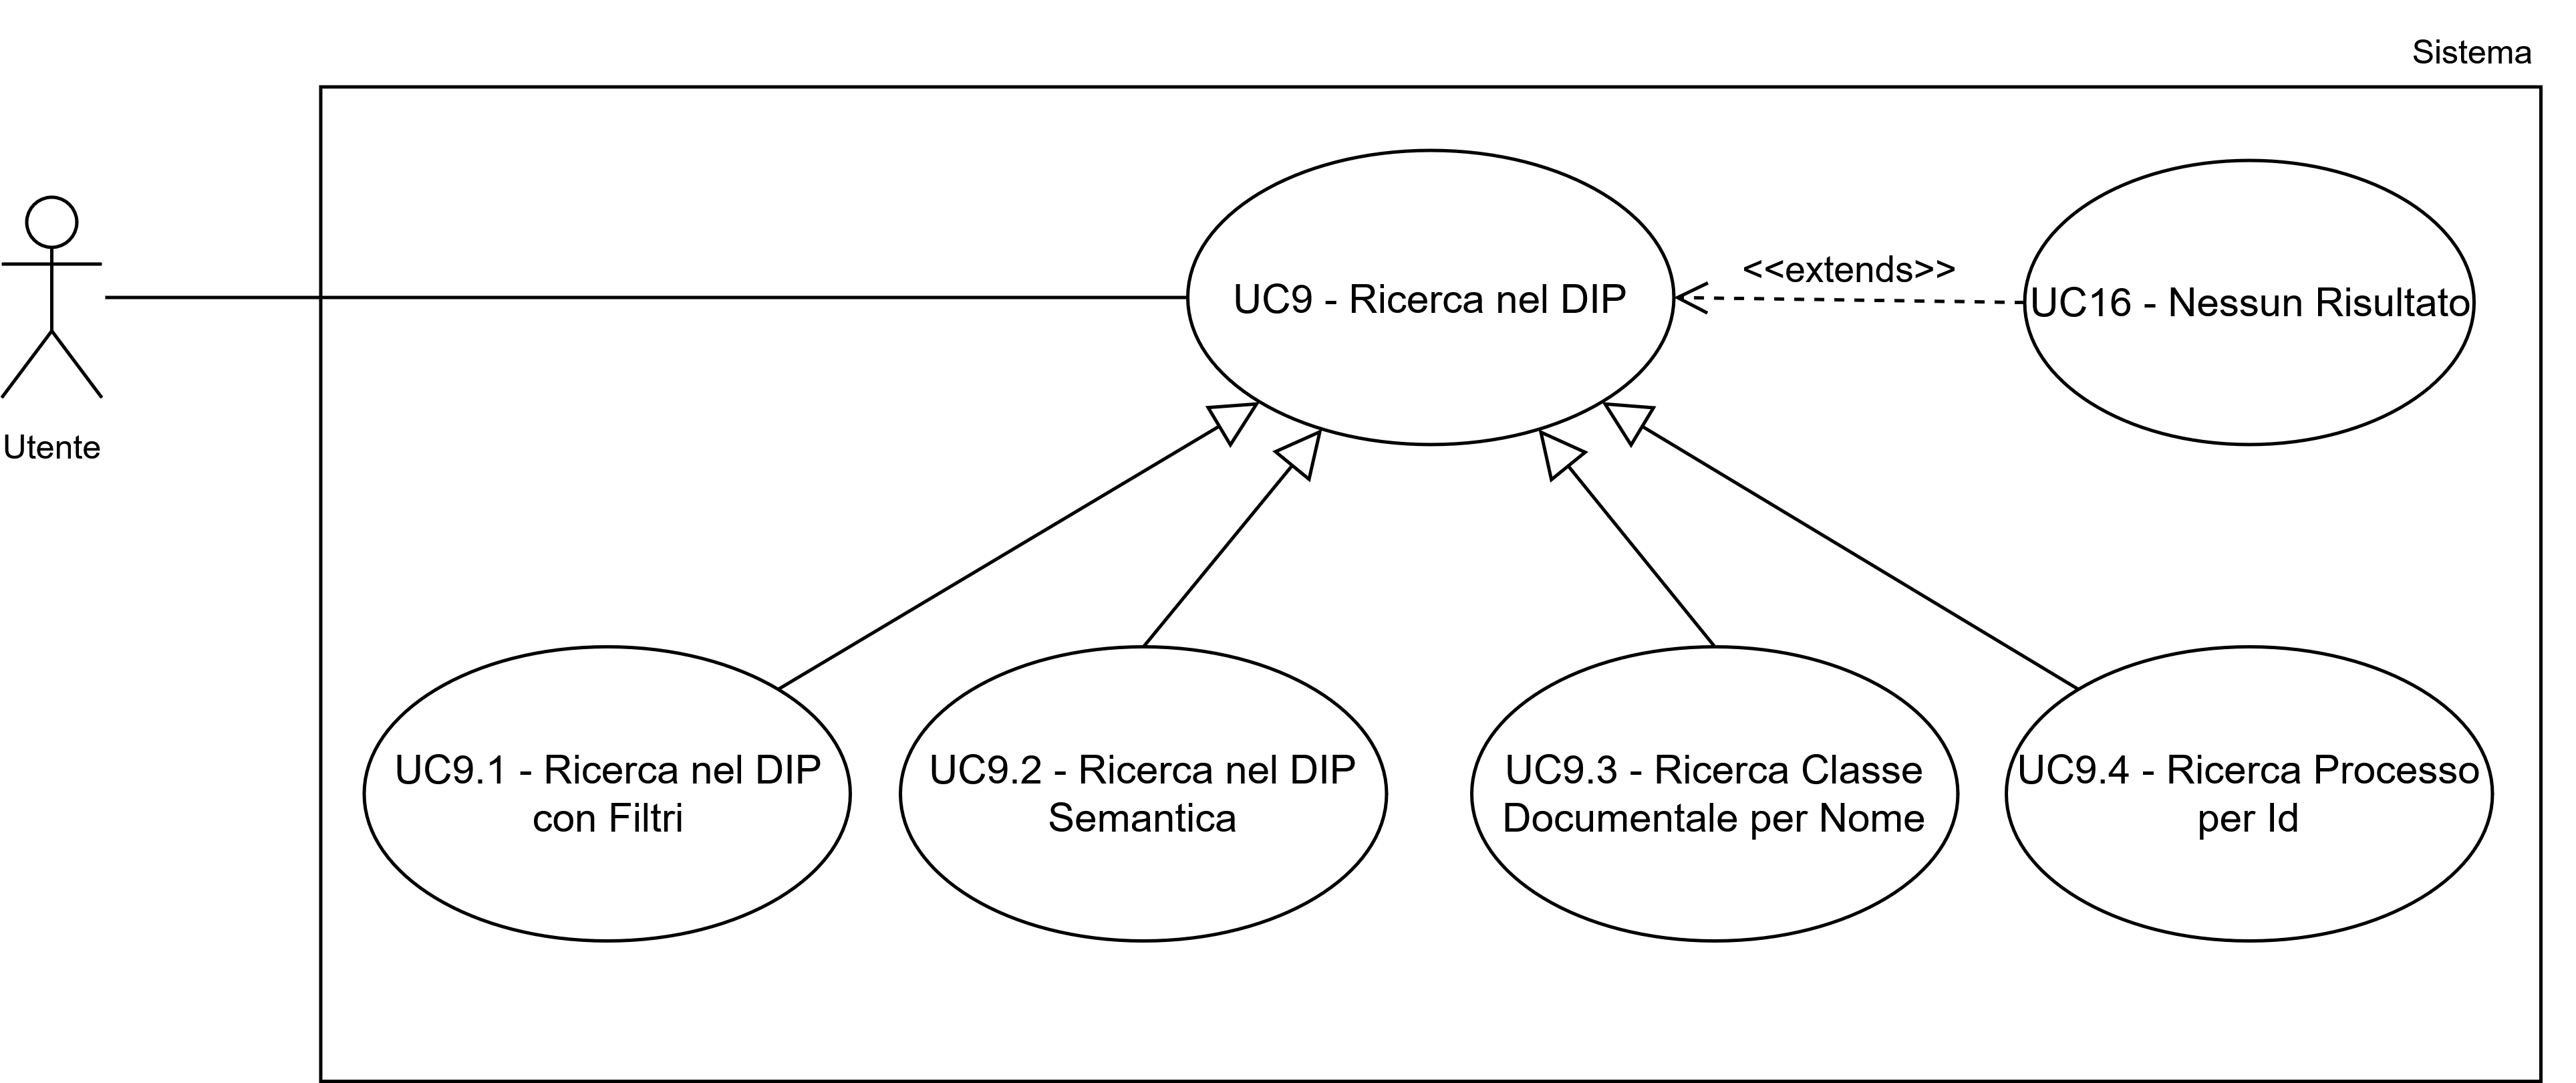
\includegraphics[width=1\textwidth]{../../assets/uml/UC9.png}
    \caption{Generalizzazione \ref{ricercaDIP} - Ricerca nel DIP}
    \label{fig:uc_ricercaDIP}
\end{figure}
\begin{itemize}
      \item \textbf{Attore Primario}: Utente
      \item \textbf{Precondizioni}: 
      \begin{itemize} 
            \item L'Utente ha avviato l'applicazione
            \item Il sistema ha indicizzato i documenti presenti nel DIP
      \end{itemize}
      \item \textbf{Postcondizioni}:
            \begin{itemize}
                  \item Il sistema produce i risultati di ricerca in base ai criteri specificati
            \end{itemize}
      \item \textbf{Flusso Principale}:
      \begin{enumerate}
            \item L'utente specifica i criteri di ricerca
            \item Il sistema produce i risultati di ricerca in base ai criteri specificati
            \item L'Utente visualizza i risultati di ricerca (\ref{visualizzaRisultati})
      \end{enumerate}
      \item \textbf{Flusso Alternativo}:
      \begin{itemize}
            \item La ricerca non produce risultati e il sistema informa l'Utente (\ref{nessunRisultato})
      \end{itemize}
      \item \textbf{Estensioni}: \ref{nessunRisultato} Nessun risultato
\end{itemize}

\subusecase{ricercaDIPConFiltri}{Ricerca nel DIP con filtri}
\begin{figure}[H]
    \centering
    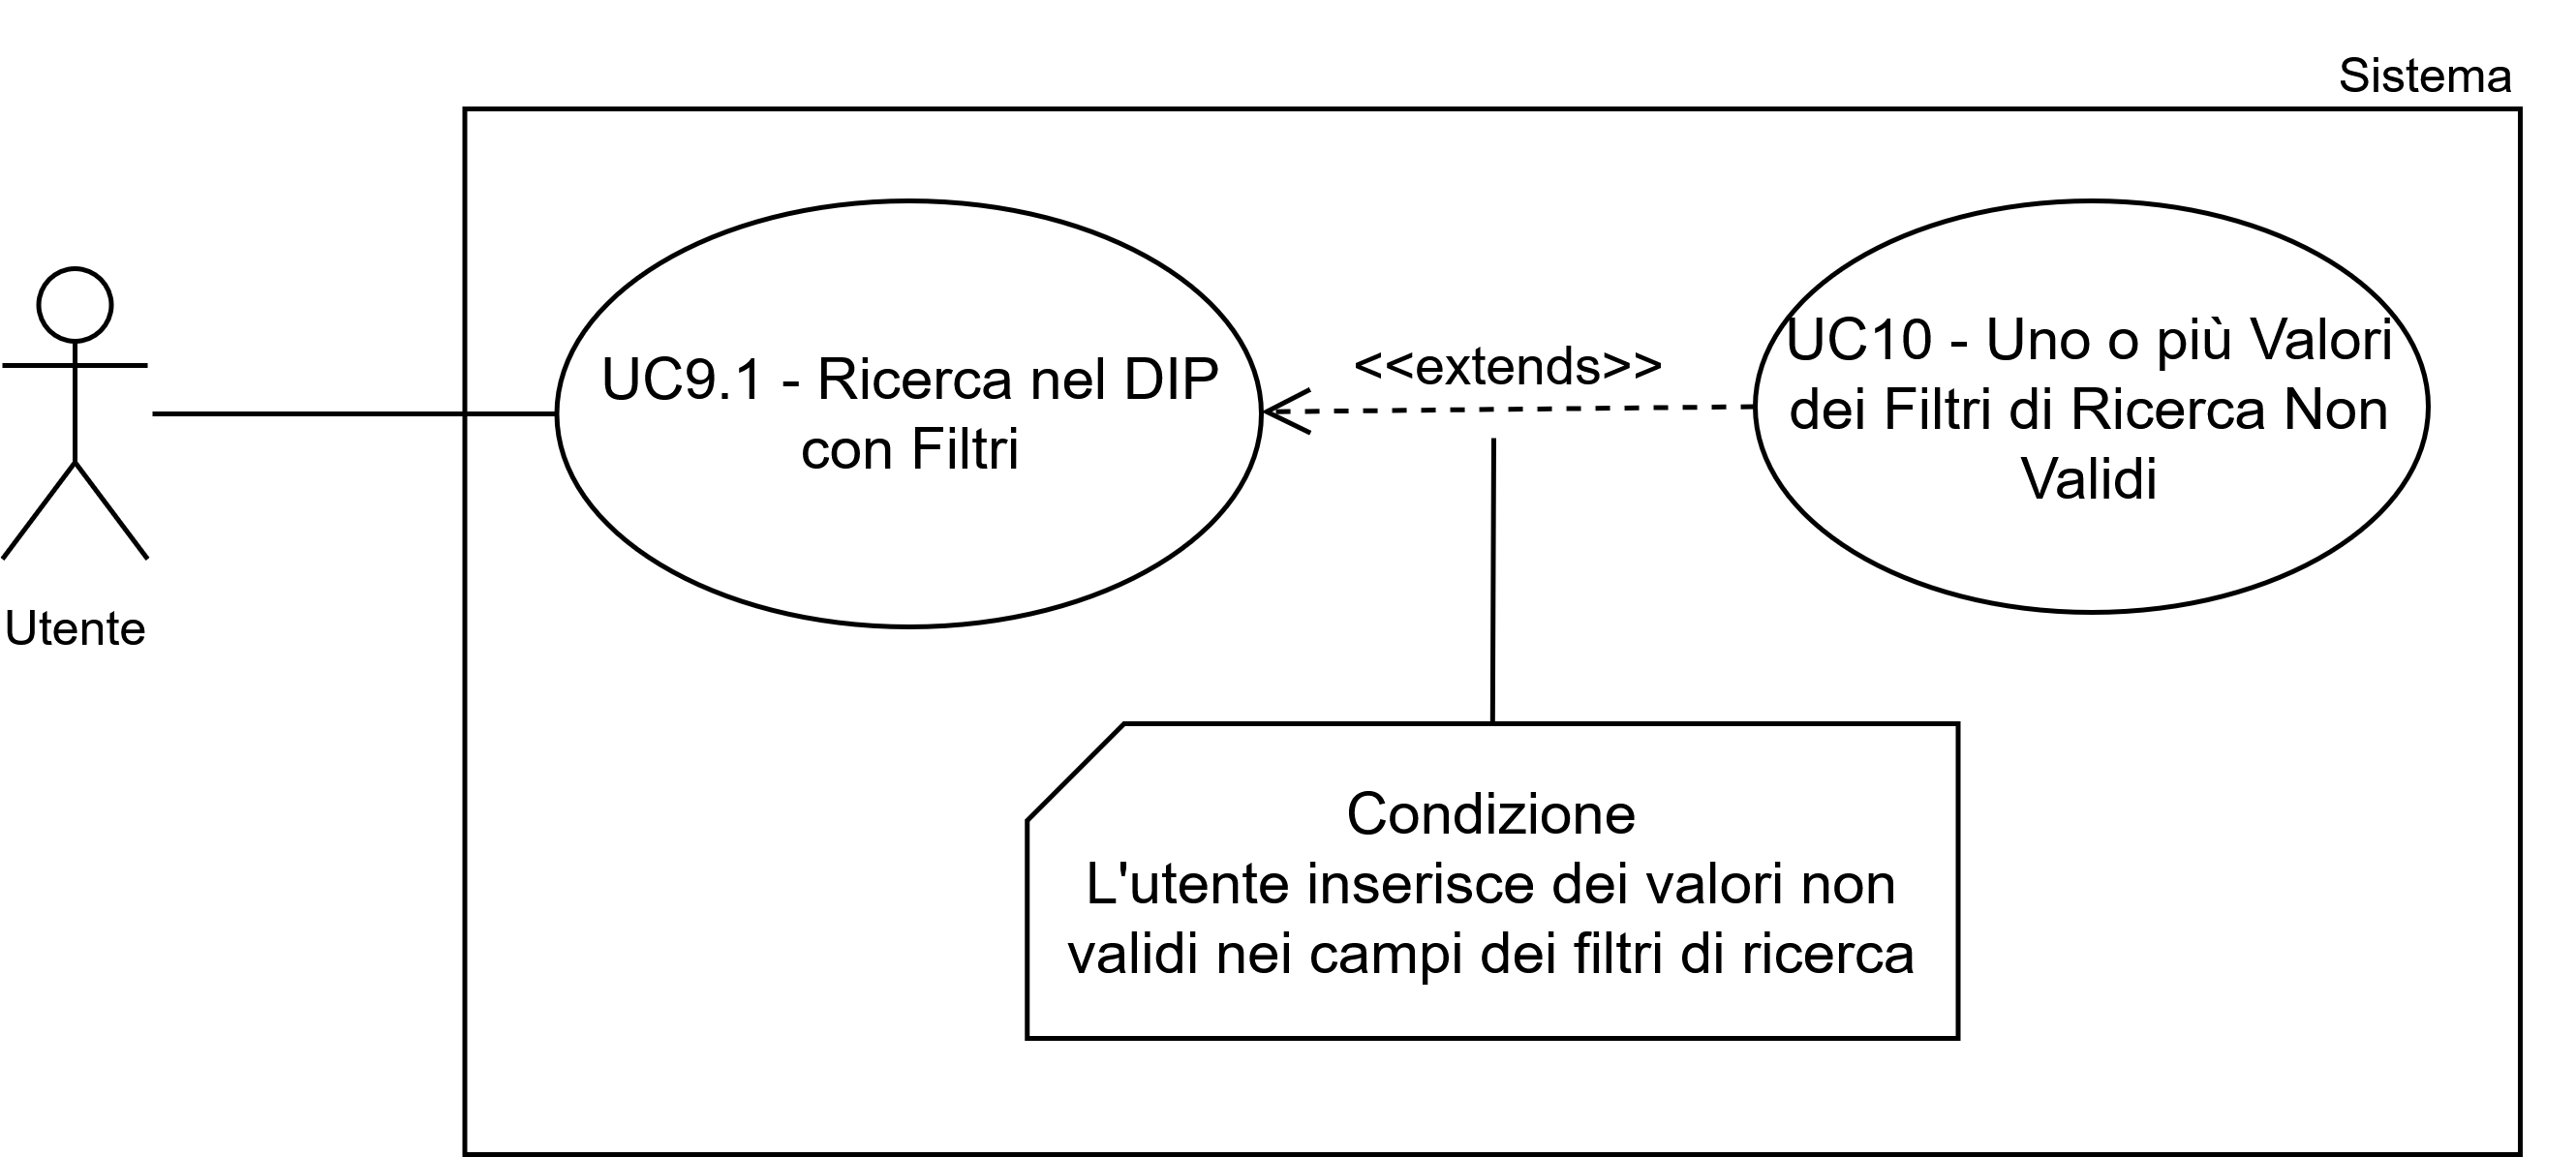
\includegraphics[width=0.9\textwidth]{../../assets/uml/UC9.1.png}
    \caption{\ref{ricercaDIPConFiltri} - Ricerca nel DIP con filtri}
    \label{fig:uc_ricercaDIPConFiltri}
\end{figure}
\begin{itemize}
      \item \textbf{Attore Primario}: Utente
      \item \textbf{Precondizioni}: 
      \begin{itemize} 
            \item L'Utente ha avviato l'applicazione
            \item Il sistema ha indicizzato i documenti presenti nel DIP
      \end{itemize}
      \item \textbf{Postcondizioni}:
            \begin{itemize}
                  \item Il sistema produce i risultati di ricerca in base ai \glossario{filtri} specificati
            \end{itemize}
      \item \textbf{Flusso Principale}:
            \begin{enumerate}
                  \item L'Utente aggiunge filtri come parametri per la ricerca  (\ref{specificaFiltriRicercaDocumento})
                  \item Vengono controllati i valori dei filtri di ricerca
                  \item Il sistema produce i risultati di ricerca in base ai filtri specificati
            \end{enumerate}
      \item \textbf{Flusso alternativo}: 
            \begin{enumerate}
                  \item Uno o più campi non rispettano i formati previsti (\ref{campoNonValido})
            \end{enumerate}
      \item \textbf{Inclusioni}: \ref{specificaFiltriRicercaDocumento} Specifica filtri per ricerca documento 
      \item \textbf{Estensioni}: \ref{campoNonValido} Uno o più valori dei filtri di ricerca non validi
      \item \textbf{Specializza}: \ref{ricercaDIP} Ricerca nel DIP
\end{itemize}
\begin{figure}[H]
      \centering
      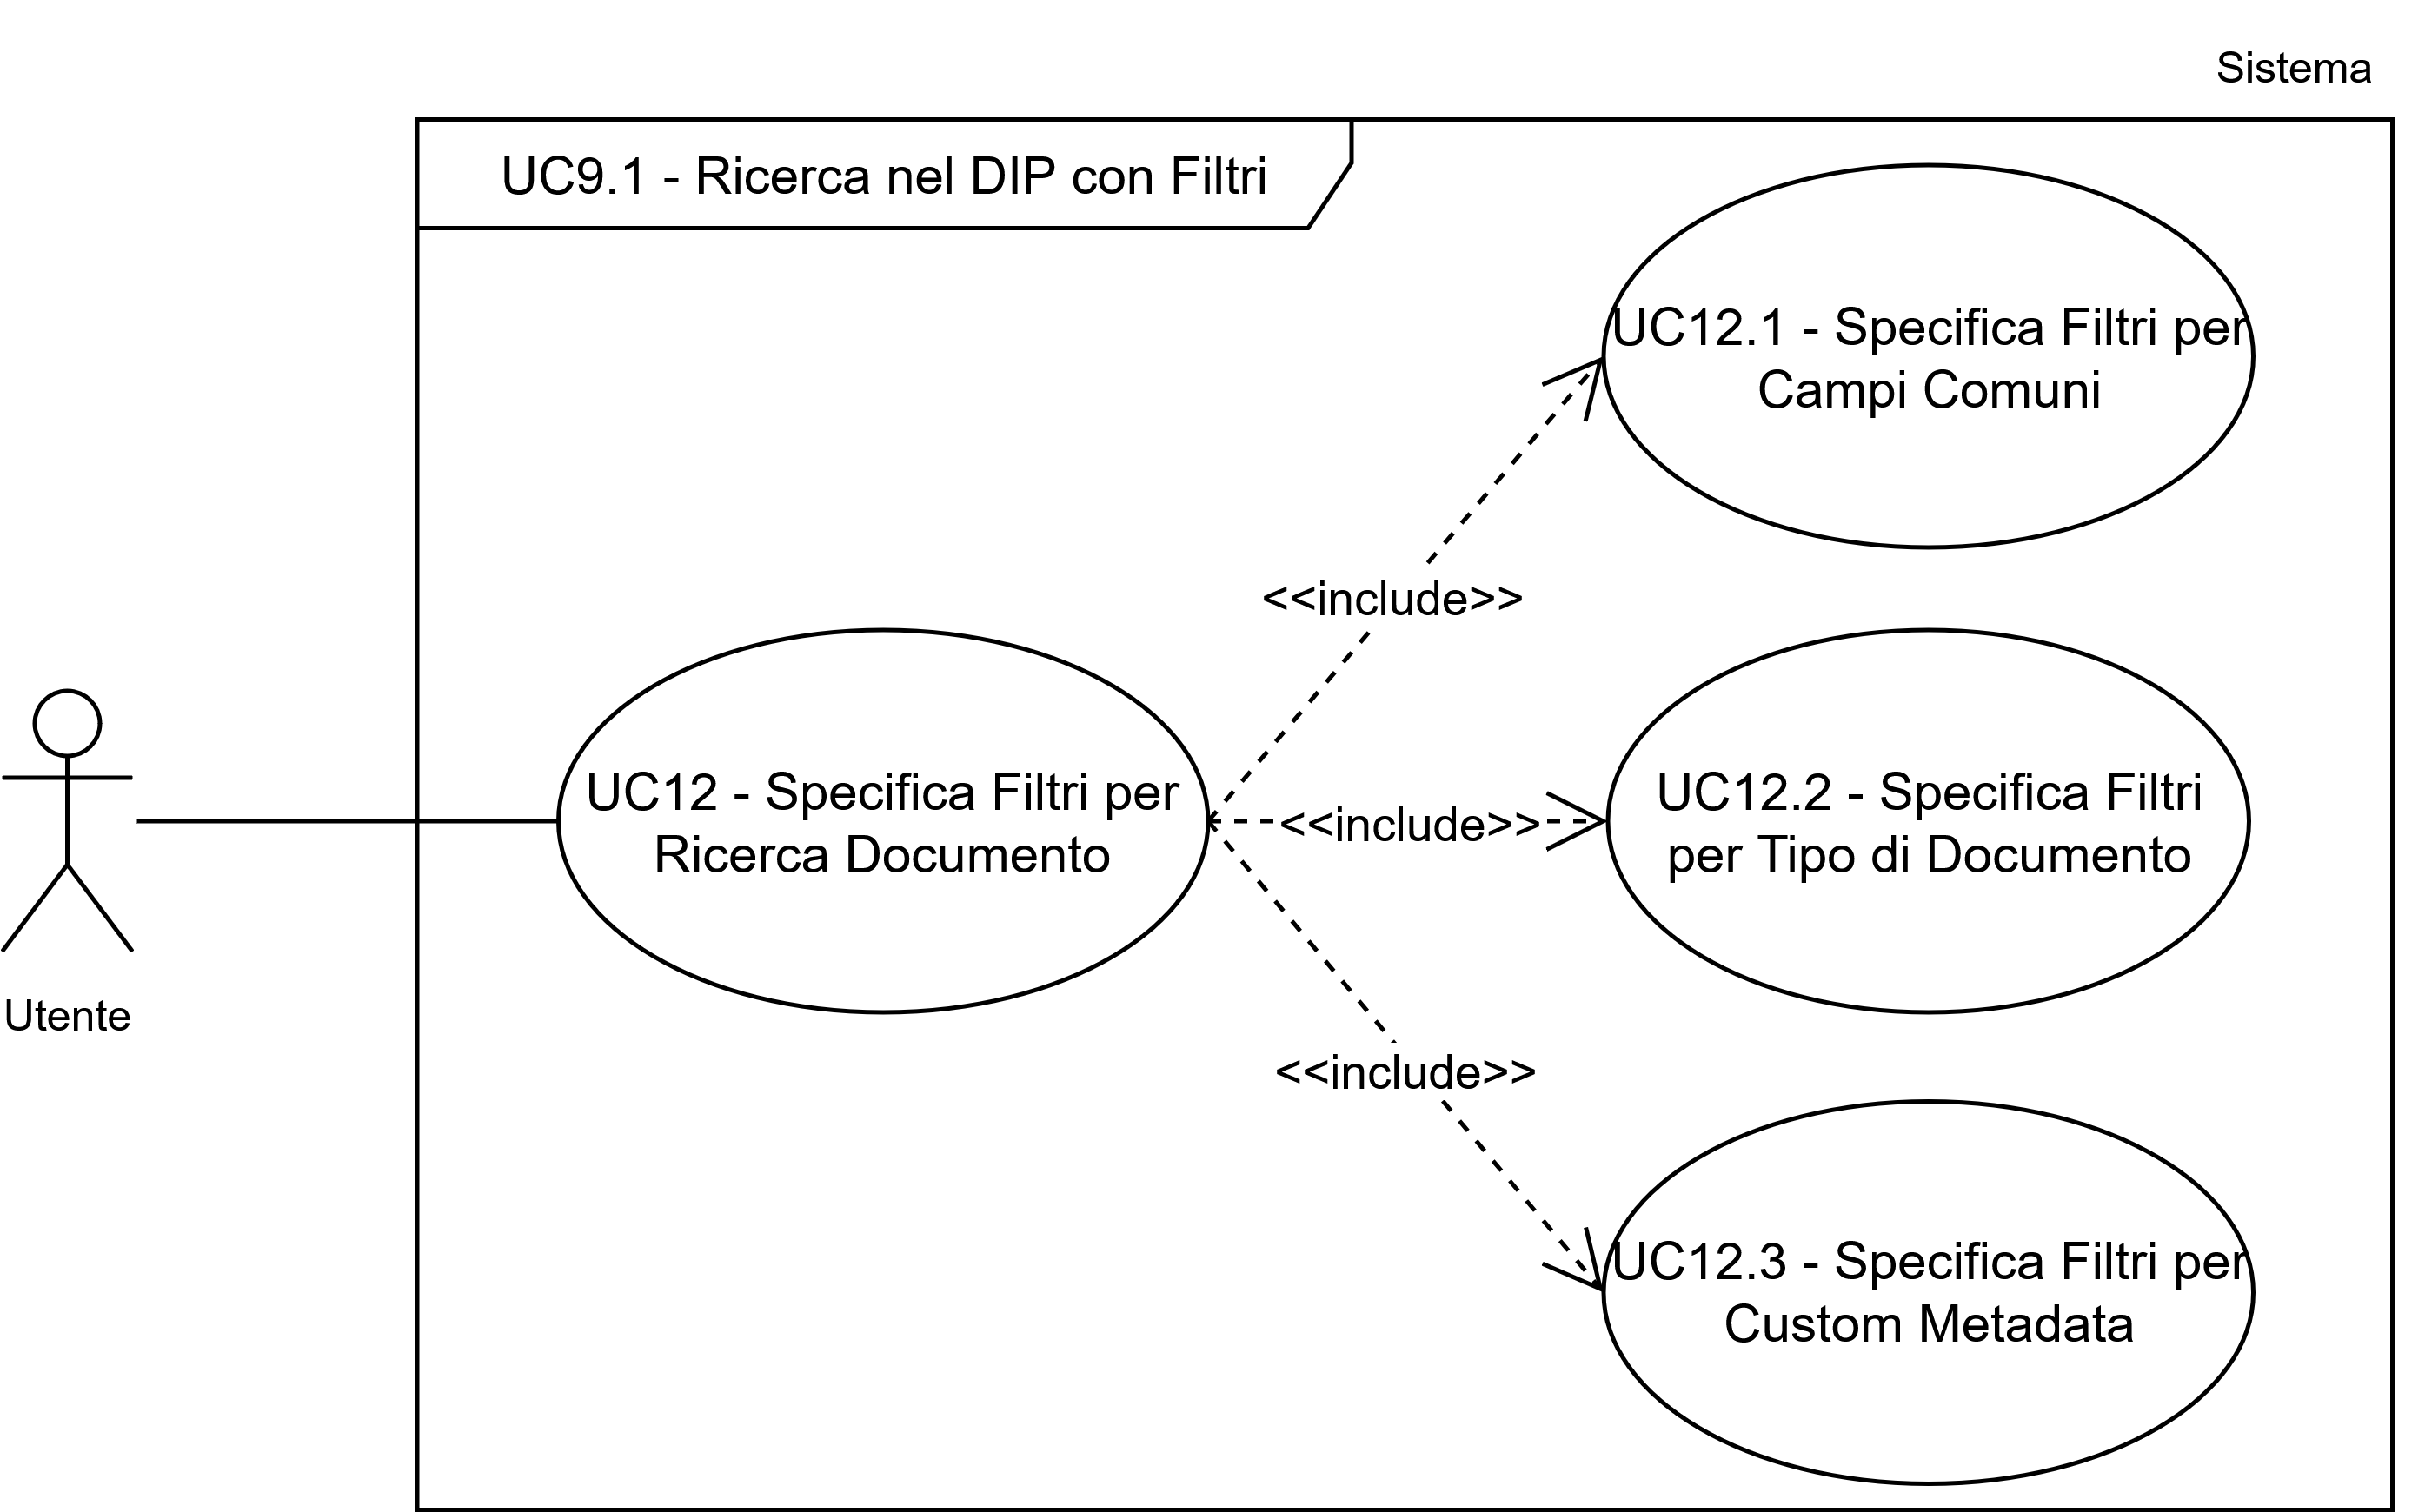
\includegraphics[width=0.9\textwidth]{../../assets/uml/UC9.1INC.png}
      \caption{Inclusioni \ref{ricercaDIPConFiltri} - Ricerca nel DIP con filtri}
      \label{fig:inclusioniRicercaDIPConFiltri}
\end{figure}

\subusecase{ricercaDIPSemantica}{Ricerca nel DIP semantica}
\begin{itemize}
    \item \textbf{Attore Primario}: Utente
    \item \textbf{Precondizioni}:
    \begin{itemize}
      \item L'Utente ha avviato l'applicazione
      \item Il sistema ha indicizzato i documenti presenti nel DIP con l'engine semantico
    \end{itemize}
    \item \textbf{Postcondizioni}:
    \begin{itemize}
        \item Il sistema produce i risultati di \glossario{ricerca semantica} per la \glossario{query} specificata.
    \end{itemize}
    \item \textbf{Flusso principale}:
    \begin{enumerate}
        \item L'Utente specifica la query di ricerca
        \item Il sistema produce i risultati di ricerca per la query specificata
    \end{enumerate}
    \item \textbf{Specializza}: \ref{ricercaDIP} Ricerca nel DIP
    
\end{itemize}

\subusecase{ricercaClasse}{Ricerca classe documentale per nome}
\begin{itemize}
      \item \textbf{Attore Primario}: Utente
      \item \textbf{Precondizioni}: 
      \begin{itemize} 
            \item L'Utente ha avviato l'applicazione
            \item Il sistema ha indicizzato i documenti presenti nel DIP
      \end{itemize}
      \item \textbf{Postcondizioni}:
            \begin{itemize}
                  \item Il sistema produce i risultati di ricerca in base al nome inserito
            \end{itemize}
      \item \textbf{Flusso Principale}:
            \begin{enumerate}
                  \item L'Utente inserisce il nome della Classe Documentale da ricercare (\ref{inserimentoNomeClasseDocumentale}).
                  \item Il sistema produce i risultati di ricerca in base al nome inserito
            \end{enumerate}

      \item \textbf{Inclusioni}: \ref{inserimentoNomeClasseDocumentale} Inserimento nome classe documentale
      \item \textbf{Specializza}: \ref{ricercaDIP} Ricerca nel DIP
\end{itemize}
\begin{figure}[H]
      \centering
      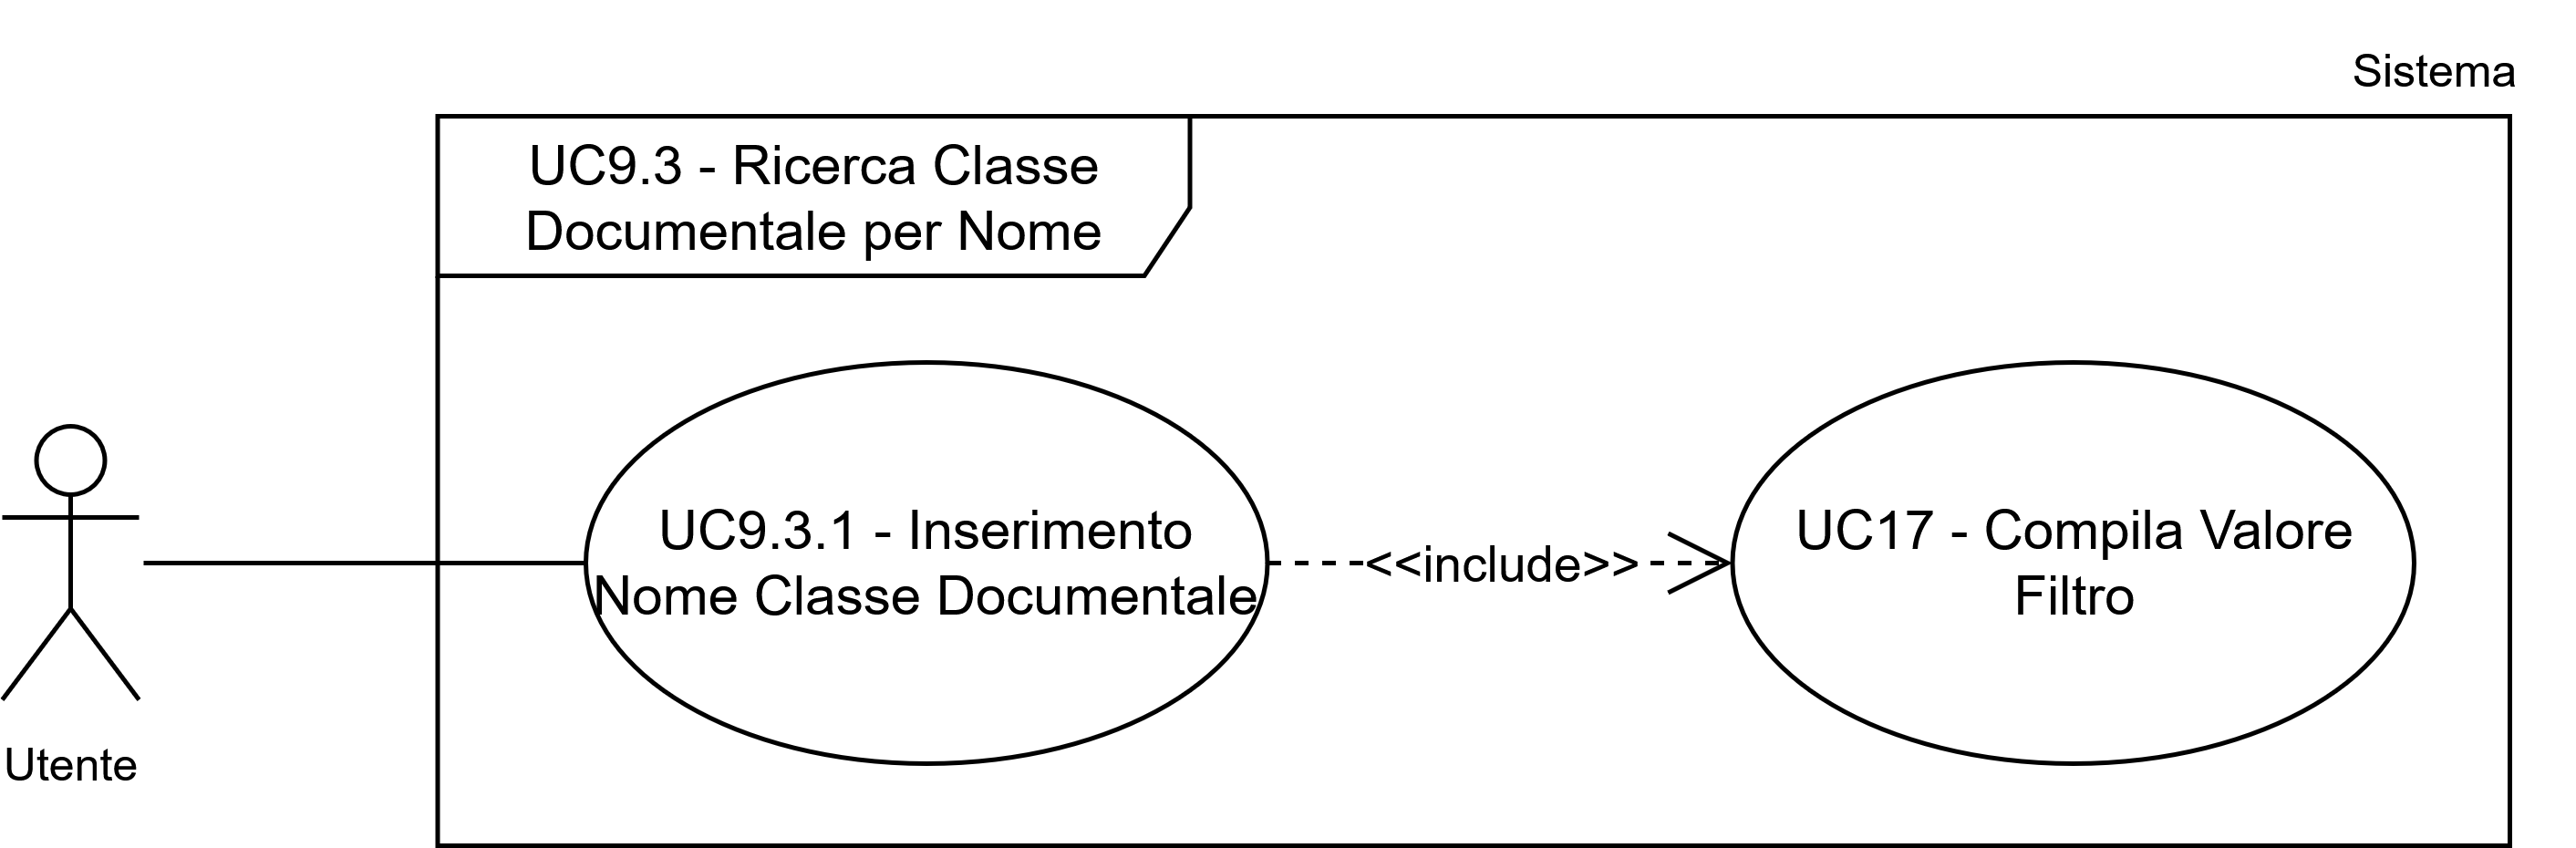
\includegraphics[width=0.9\textwidth]{../../assets/uml/UC9.3INC.png}
      \caption{Inclusioni \ref{ricercaClasse} - Ricerca classe documentale per nome}
      \label{fig:inclusioniRicercaClasse}
\end{figure}

\subsubusecase{inserimentoNomeClasseDocumentale}{Inserimento nome classe documentale}
\begin{itemize}
      \item \textbf{Attore Primario}: Utente
      \item \textbf{Precondizioni}:
      \begin{itemize}
            \item L'Utente ha avviato l'applicazione
            \item L'Utente sta effettuando una ricerca nel DIP per Classe Documentale
      \end{itemize}
      \item \textbf{Postcondizioni}: Il sistema riceve il nome della Classe Documentale che l'Utente vuole ricercare.
      \item \textbf{Flusso Principale}:
      \begin{enumerate}
            \item L'Utente inserisce il nome della Classe Documentale da ricercare
            \item Il sistema riceve il nome della Classe Documentale
      \end{enumerate}
\end{itemize}

\subusecase{ricercaProcesso}{Ricerca processo per Id}
\begin{itemize}
      \item \textbf{Attore Primario}: Utente
      \item \textbf{Precondizioni}: \begin{itemize}
            \item L'Utente ha avviato l'applicazione
            \item Il sistema ha indicizzato i documenti presenti nel DIP
      \end{itemize}
      \item \textbf{Postcondizioni}: Il sistema produce i risultati di ricerca in base all'Id inserito
      \item \textbf{Flusso Principale}:
      \begin{enumerate}
            \item L'Utente inserisce l'Id del Processo (\ref{inserimentoIdProcesso})
            \item Il sistema produce i risultati di ricerca in base all'Id inserito
      \end{enumerate}
      \item \textbf{Inclusioni}: \ref{inserimentoIdProcesso} Inserimento Id processo
      \item \textbf{Specializza}: \ref{ricercaDIP} Ricerca nel DIP
\end{itemize}
\begin{figure}[H]
      \centering
      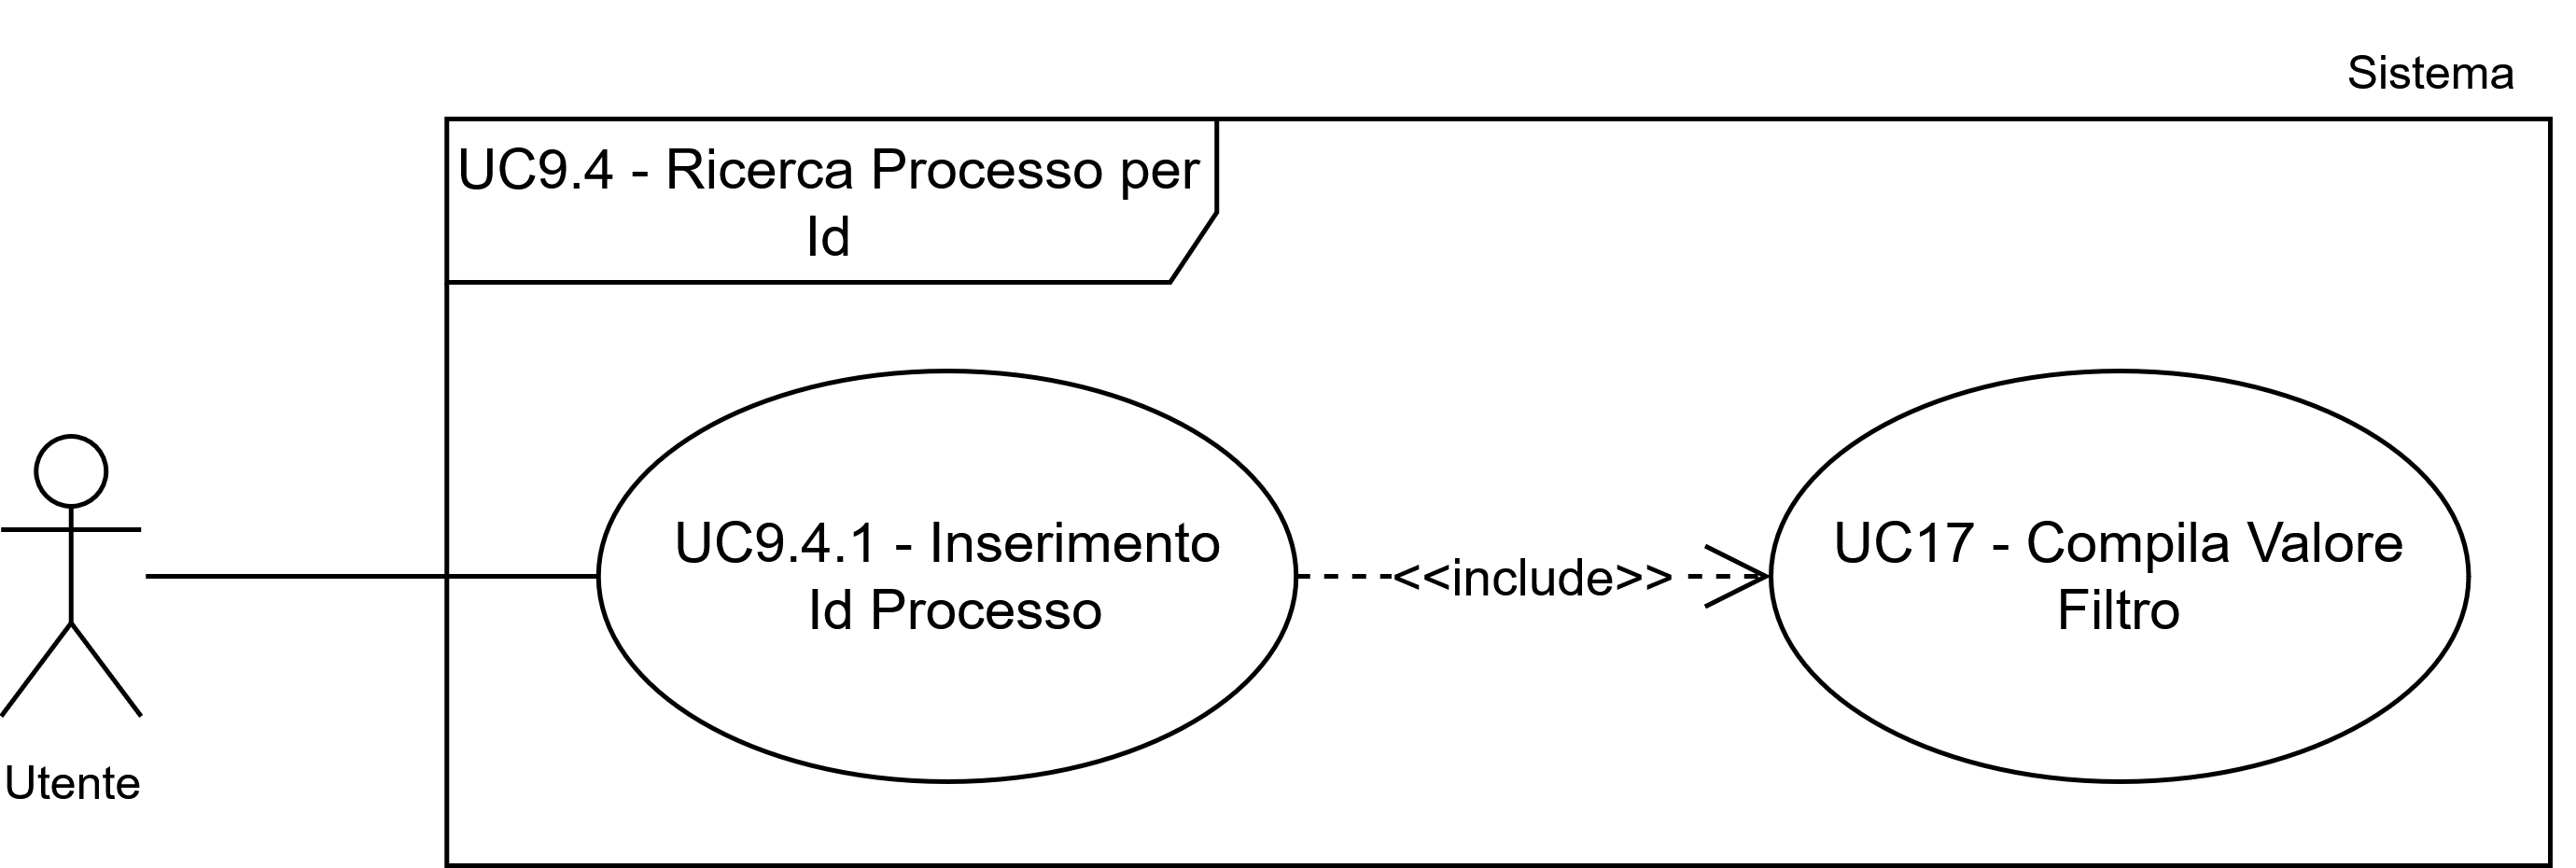
\includegraphics[width=0.9\textwidth]{../../assets/uml/UC9.4INC.png}
      \caption{Inclusioni \ref{ricercaProcesso} - Ricerca processo per Id}
      \label{fig:inclusioniRicercaProcesso}
\end{figure}

\subsubusecase{inserimentoIdProcesso}{Inserimento Id processo}
\begin{itemize}
      \item \textbf{Attore Primario}: Utente
      \item \textbf{Precondizioni}:
      \begin{itemize}
            \item L'Utente ha avviato l'applicazione
            \item L'Utente sta effettuando una ricerca nel DIP per Processo
      \end{itemize}
      \item \textbf{Postcondizioni}:
      \begin{itemize}
            \item Il sistema riceve l'Id del Processo che l'Utente vuole ricercare
      \end{itemize}
      \item \textbf{Flusso Principale}:
      \begin{enumerate}
            \item L'Utente inserisce l'Id del Processo da ricercare
            \item Il sistema riceve l'Id del Processo
      \end{enumerate}
\end{itemize}

\usecase{campoNonValido}{Uno o più valori dei filtri di ricerca non validi}
\begin{itemize}
      \item \textbf{Attore Primario}: Sistema
      \item \textbf{Precondizioni}: 
      \begin{itemize}
            \item L'Utente ha avviato l'applicazione
            \item L'Utente sta effettuando una ricerca nel DIP con filtri
      \end{itemize}
      \item \textbf{Postcondizioni}: Il sistema annulla la ricerca mostrando un messaggio di errore che indica i campi non validi
      \item \textbf{Flusso Principale}:
      \begin{enumerate}
            \item Il sistema annulla l'operazione di ricerca
            \item Il sistema mostra a video un messaggio di errore che indica quali campi non rispettano i formati previsti
      \end{enumerate}
\end{itemize}


\usecase{StatoIndicizzazione}{Visualizza stato indicizzazione semantica}
\begin{figure}[H]
    \centering
    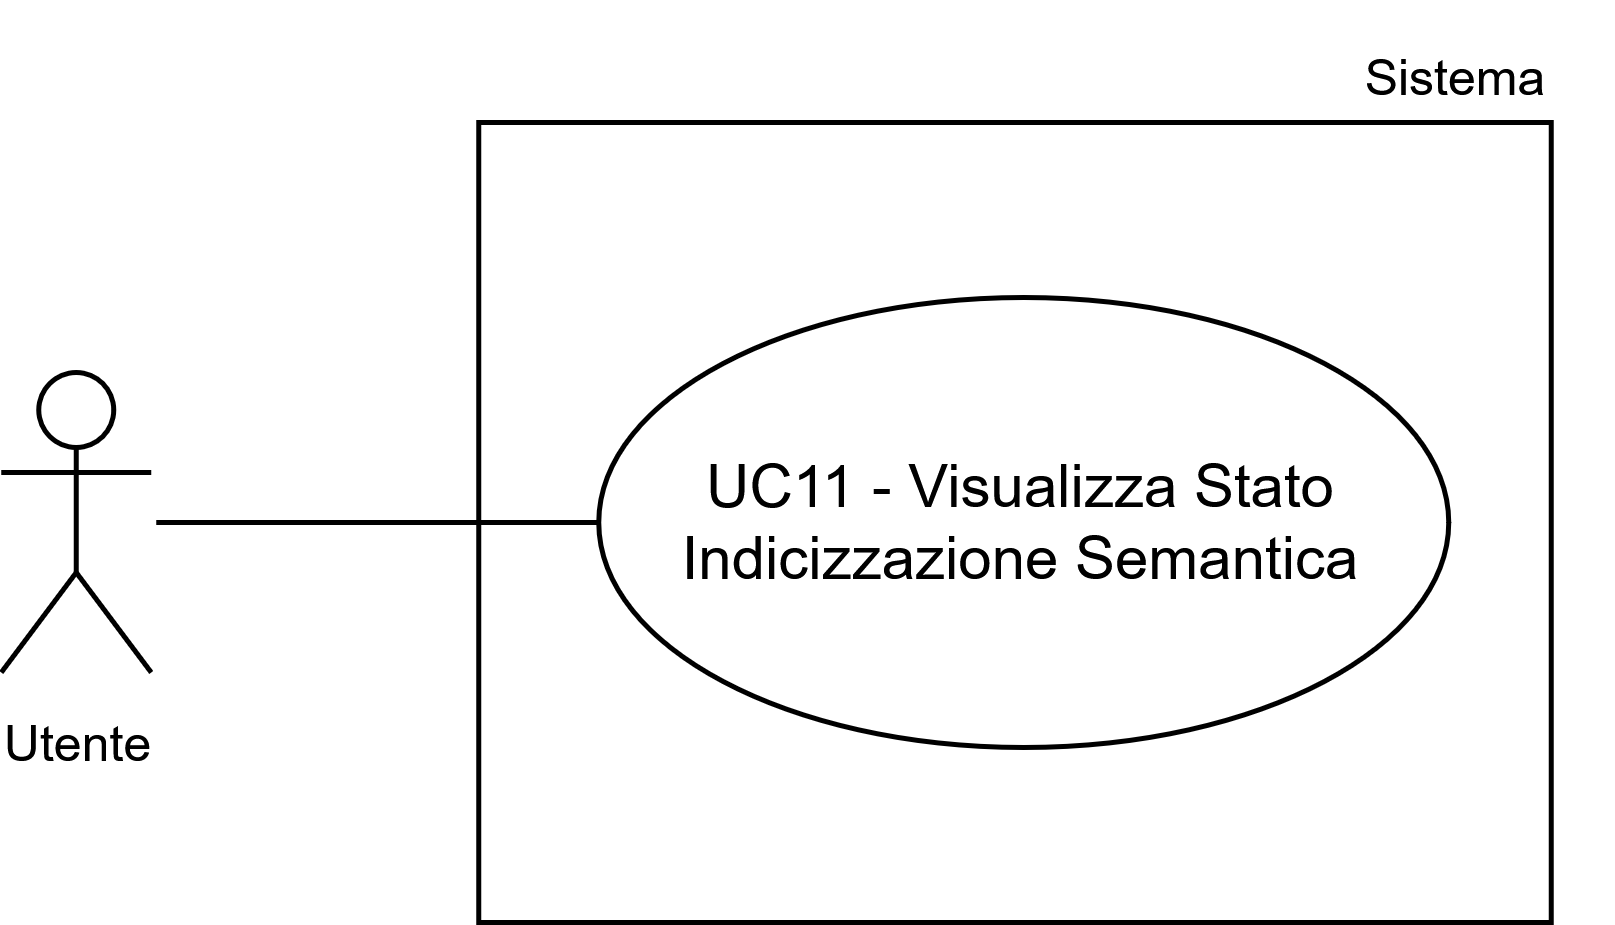
\includegraphics[width=0.6\textwidth]{../../assets/uml/UC11.png}
    \caption{\ref{StatoIndicizzazione} - Visualizza stato indicizzazione semantica}
    \label{fig:uc_statoIndicizzazione}
\end{figure}
\begin{itemize}
    \item \textbf{Attore Primario}: Utente
    \item \textbf{Precondizioni}:
    \begin{itemize}
      \item L'Utente ha avviato l'applicazione
      \item L'Utente ha selezionato l'opzione di \glossario{indicizzazione} semantica
    \end{itemize}
    \item \textbf{Postcondizioni}:
    \begin{itemize}
        \item L'Utente vede lo stato di indicizzazione per la ricerca semantica
    \end{itemize}
    \item \textbf{Flusso principale}:
    \begin{enumerate}
        \item L'Utente visualizza un messaggio di notifica lo stato della Ricerca Semantica.
    \end{enumerate}
\end{itemize}

\subusecase{StatoIndicizzazioneCompletata}{Visualizza stato indicizzazione semantica "Completata"}
\begin{itemize}
    \item \textbf{Attore Primario}: Utente
    \item \textbf{Precondizioni}:
    \begin{itemize}
      \item L'Utente ha avviato l'applicazione
      \item L'Utente ha selezionato l'opzione di \glossario{indicizzazione} semantica
      \item L'indicizzazione semantica è stata completata
    \end{itemize}
    \item \textbf{Postcondizioni}:
    \begin{itemize}
        \item L'Utente vede lo stato di indicizzazione per la ricerca semantica "Completata"
    \end{itemize}
    \item \textbf{Flusso principale}:
    \begin{enumerate}
        \item L'Utente visualizza un messaggio di notifica lo stato della Ricerca Semantica "Completata".
    \end{enumerate}
    \item \textbf{Specializza}:
    \begin{enumerate}
              \item \ref{StatoIndicizzazione} Visualizza stato indicizzazione semantica
    \end{enumerate}
\end{itemize}

\subusecase{StatoIndicizzazioneNonCompletata}{Visualizza stato indicizzazione semantica "Non completata"}
\begin{itemize}
    \item \textbf{Attore Primario}: Utente
    \item \textbf{Precondizioni}:
    \begin{itemize}
      \item L'Utente ha avviato l'applicazione
      \item L'Utente ha selezionato l'opzione di \glossario{indicizzazione} semantica
      \item L'indicizzazione semantica non è stata completata
    \end{itemize}
    \item \textbf{Postcondizioni}:
    \begin{itemize}
        \item L'Utente vede lo stato di indicizzazione per la ricerca semantica "Non completata"
    \end{itemize}
    \item \textbf{Flusso principale}:
    \begin{enumerate}
        \item L'Utente visualizza un messaggio di notifica lo stato della Ricerca Semantica "Non completata".
    \end{enumerate}
    \item \textbf{Specializza}:
    \begin{enumerate}
              \item \ref{StatoIndicizzazione} Visualizza stato indicizzazione semantica
    \end{enumerate}
\end{itemize}

\usecase{specificaFiltriRicercaDocumento}{Specifica filtri per ricerca documento}
\begin{itemize}
      \item \textbf{Attore Primario}: Utente
      \item \textbf{Precondizioni}: 
      \begin{itemize}
            \item L'Utente ha avviato l'applicazione
            \item L'Utente sta effettuando una ricerca nel DIP con filtri
      \end{itemize}
      \item \textbf{Postcondizioni}: Vengono specificati i filtri per la ricerca dei documenti.
      \item \textbf{Flusso Principale}:
      \begin{enumerate}
            \item L'Utente specifica i filtri per la ricerca tra \glossario{campi comuni} (\ref{specificaFiltriComuni})
            \item L'Utente specifica i filtri per la ricerca tra campi specifici per tipo documentale (\ref{addFiltriTipoDocumento})
            \item L'Utente specifica i filtri per i \glossario{custom metadata} (\ref{addCustomMetadata})
      \end{enumerate}
      \item \textbf{Inclusioni}: 
      \begin{itemize}
            \item \ref{specificaFiltriComuni} Specifica filtri per campi comuni
            \item \ref{addFiltriTipoDocumento} Specifica filtri per tipo di documento
            \item \ref{addCustomMetadata} Specifica filtri per custom metadata
      \end{itemize}
\end{itemize}

\subusecase{specificaFiltriComuni}{Specifica filtri per campi comuni}
\begin{itemize}
      \item \textbf{Attore Primario}: Utente
      \item \textbf{Precondizioni}:\begin{itemize}
            \item L'Utente ha avviato l'applicazione
            \item L'Utente sta effettuando una ricerca nel DIP con filtri
      \end{itemize}
      \item \textbf{Postcondizioni}: Vengono specificati i filtri per i campi comuni per la ricerca dei documenti e utilizzati per la generazione del risultato.
      \item \textbf{Flusso Principale}:
      \begin{enumerate}
            \item L'Utente seleziona i campi comuni su cui basare la ricerca. (\ref{selezionaCampiRicercaComuni})
            \item L'Utente specifica i filtri per i campi selezionati (da \ref{addChiaveDescrittiva} a \ref{addSoggetti})
      \end{enumerate}
      \item \textbf{Inclusioni}: 
      \begin{itemize}
            \item \ref{selezionaCampiRicercaComuni} Seleziona campi di ricerca comuni
            \item \ref{addChiaveDescrittiva} Specifica filtro Chiave Descrittiva
            \item \ref{addClassificazione} Specifica filtro Classificazione
            \item \ref{addTempoConserva} Specifica filtro \glossario{Tempo di Conservazione}
            \item \ref{addNote} Specifica filtro Note
            \item \ref{addTipoDocumento} Specifica filtro Tipo documento
            \item \ref{addSoggetti} Specifica filtro \glossario{Soggetti}
      \end{itemize}
\end{itemize}
\begin{figure}[H]
      \centering
      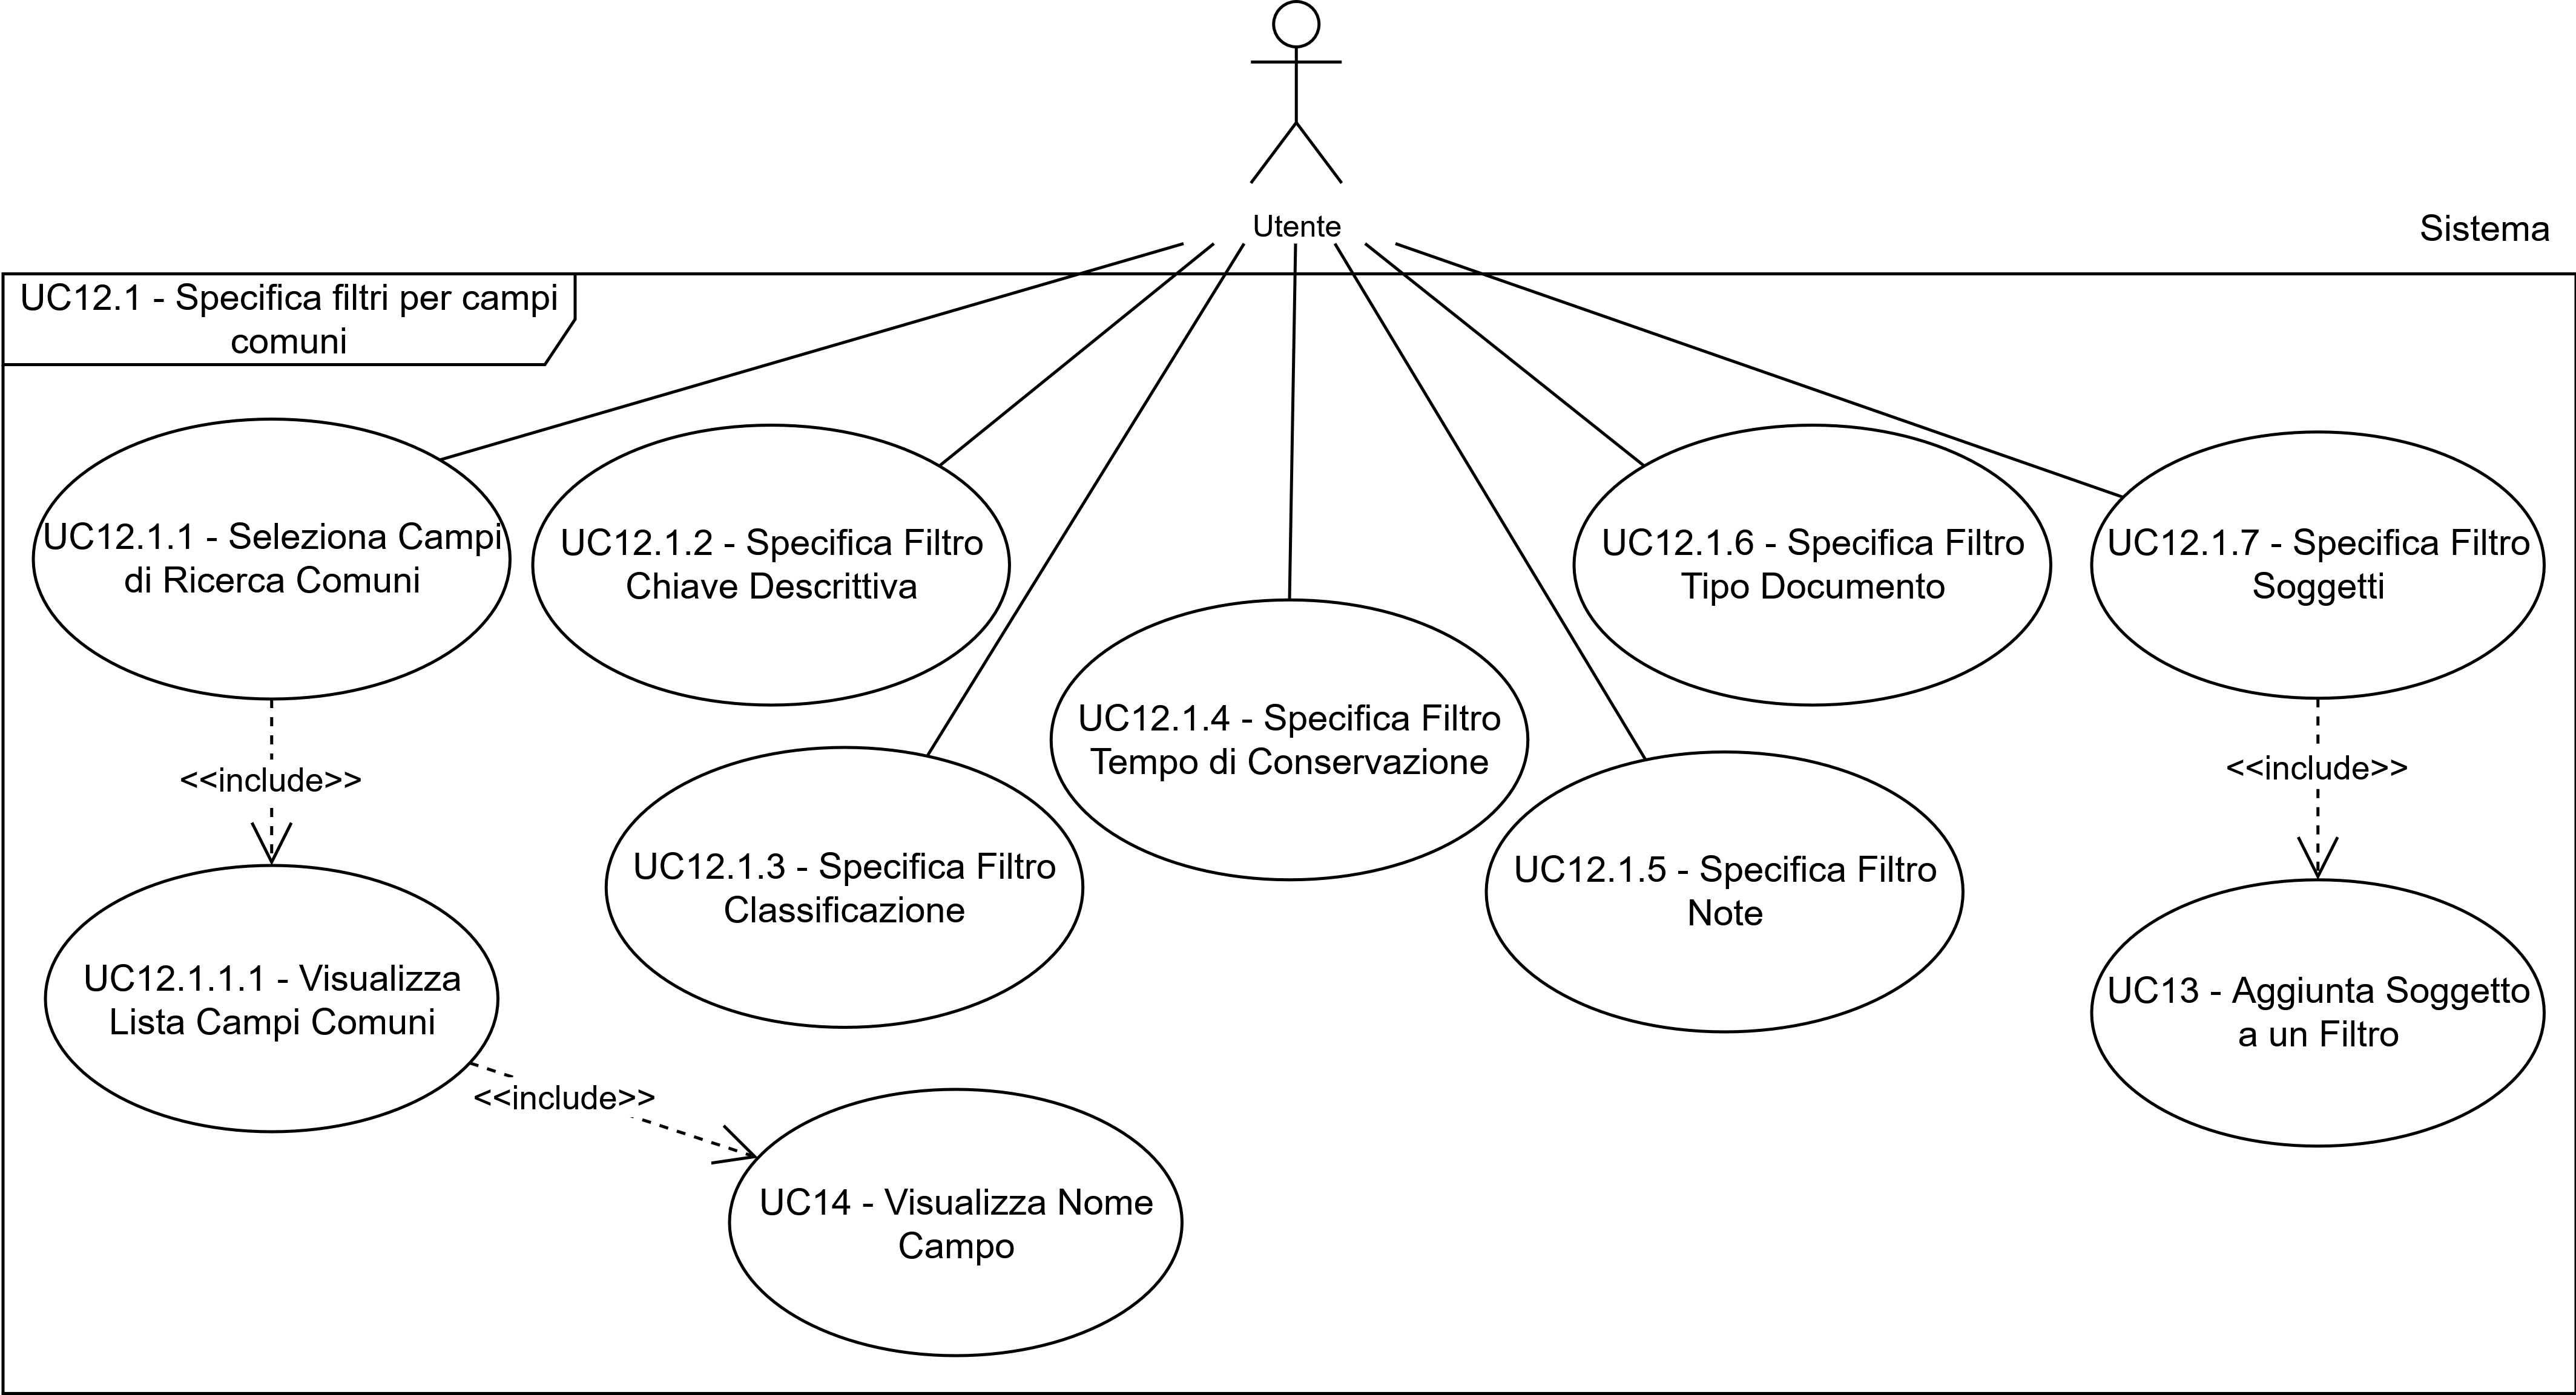
\includegraphics[width=1\textwidth]{../../assets/uml/UC12.1INC.png}
      \caption{\ref{specificaFiltriComuni} - Specifica filtri per campi comuni}
      \label{fig:uc_specificaFiltriComuni}
\end{figure}

\subsubusecase{selezionaCampiRicercaComuni}{Selezione campi di ricerca comuni}
\begin{itemize}
      \item \textbf{Attore Primario}: Utente
      \item \textbf{Precondizioni}: \begin{itemize}
            \item L'Utente ha avviato l'applicazione
            \item L'Utente sta effettuando una ricerca nel DIP con filtri
      \end{itemize}
      \item \textbf{Postcondizioni}:  I campi selezionati dall'Utente sono aggiunti ai campi selezionati per la ricerca.
      \item \textbf{Flusso Principale}:
      \begin{enumerate}
            \item L'Utente sceglie uno o più campi tra quelli disponibili
            \item Il sistema aggiunge gli elementi selezionati ai campi selezionati per la ricerca
      \end{enumerate}
\end{itemize}

\subsubusecase{addChiaveDescrittiva}{Specifica filtro Chiave Descrittiva}
\begin{itemize}
      \item \textbf{Attore Primario}: Utente
      \item \textbf{Precondizioni}: \begin{itemize}
            \item L'Utente ha avviato l'applicazione
            \item L'Utente sta effettuando una ricerca nel DIP con filtri
            \item L'Utente ha selezionato il filtro Chiave Descrittiva tra i campi comuni
      \end{itemize}
      \item \textbf{Postcondizioni}: \begin{itemize}
            \item L'Utente ha specificato i valori del filtro Chiave Descrittiva
            \item Il filtro Chiave Descrittiva è parametro per la ricerca con filtri e per la generazione del risultato
      \end{itemize}
      \item \textbf{Flusso Principale}:
            \begin{enumerate}
                  \item L'Utente compila i valori di Chiave Descrittiva quali:
                        \begin{itemize}
                              \item Oggetto (\ref{addValoreOggetto})
                              \item Parole Chiave (\ref{addValoreParoleChiave})
                        \end{itemize}
                  \item Il sistema imposta i valori del filtro come parametri di ricerca.
            \end{enumerate}
      \item \textbf{Inclusioni}: 
      \begin{itemize} 
            \item \ref{addValoreOggetto} - Specifica valore Oggetto
            \item \ref{addValoreParoleChiave} - Specifica valore Parole Chiave
      \end{itemize}
\end{itemize}

\deepusecase{addValoreOggetto}{Specifica valore Oggetto}\label{addValoreOggetto}
\begin{itemize}
      \item \textbf{Attore Primario}: Utente
      \item \textbf{Precondizioni}: 
      \begin{itemize}
            \item L'Utente ha avviato l'applicazione
            \item L'Utente sta effettuando una ricerca nel DIP con filtri
            \item L'Utente ha selezionato il filtro Chiave Descrittiva tra i campi comuni
      \end{itemize}
      \item \textbf{Postcondizioni}: Il sistema riceve il valore del campo Oggetto e lo salva per il filtro Chiave Descrittiva.
      \item \textbf{Flusso Principale}:
      \begin{enumerate}
            \item L'Utente compila il valore del campo Oggetto (alfanumerico).
            \item Il sistema riceve il valore del campo Oggetto e lo salva per il filtro Chiave Descrittiva.
      \end{enumerate}
      \item \textbf{Flusso Alternativo}:
      \begin{itemize}
            \item La stringa inserita è vuota o composta da soli spazi (\ref{formatoNonCorrettoStringa})
      \end{itemize}
      \item \textbf{Estensioni}: \ref{formatoNonCorrettoStringa} Formato non corretto: stringa
\end{itemize}

\deepusecase{addValoreParoleChiave}{Specifica valore Parole Chiave}\label{addValoreParoleChiave}
\begin{itemize}
      \item \textbf{Attore Primario}: Utente
      \item \textbf{Precondizioni}: 
      \begin{itemize}
            \item L'Utente ha avviato l'applicazione
            \item L'Utente sta effettuando una ricerca nel DIP con filtri
            \item L'Utente ha selezionato il filtro Chiave Descrittiva tra i campi comuni
      \end{itemize}
      \item \textbf{Postcondizioni}: Il sistema riceve il valore del campo Parole Chiave e lo salva per il filtro Chiave Descrittiva.
      \item \textbf{Flusso Principale}:
      \begin{enumerate}
            \item L'Utente compila il valore del campo Parole Chiave (alfanumerico).
            \item Il sistema riceve il valore del campo Parole Chiave e lo salva per il filtro Chiave Descrittiva.
      \end{enumerate}
      \item \textbf{Flusso Alternativo}:
      \begin{itemize}
            \item La stringa inserita è vuota o composta da soli spazi (\ref{formatoNonCorrettoStringa})
      \end{itemize}
      \item \textbf{Estensioni}: \ref{formatoNonCorrettoStringa} Formato non corretto: stringa
\end{itemize}

\subsubusecase{addClassificazione}{Specifica filtro Classificazione}
\begin{itemize}
      \item \textbf{Attore Primario}: Utente
      \item \textbf{Precondizioni}:  \begin{itemize}
            \item L'Utente ha avviato l'applicazione
            \item L'Utente sta effettuando una ricerca nel DIP con filtri
            \item L'Utente ha selezionato il filtro Classificazione tra i campi comuni
      \end{itemize}
      \item \textbf{Postcondizioni}: \begin{itemize}
            \item L'Utente ha specificato i valori del filtro Classificazione
            \item Il filtro Classificazione è parametro per la ricerca con filtri e per la generazione del risultato
      \end{itemize}
      \item \textbf{Flusso Principale}:
            \begin{enumerate}
                  \item L'Utente compila i valori di Classificazione tra:
                        \begin{itemize}
                              \item \glossario{Indice di Classificazione}
                              \item Descrizione
                              \item \glossario{URI Piano di Classificazione}
                        \end{itemize}
                  \item Il sistema imposta i valori del filtro come parametri di ricerca.
            \end{enumerate}
      \item \textbf{Inclusioni}: \begin{itemize}
            \item \ref{addValoreIndiceDiClassificazione} Specifica valore Indice di Classificazione
            \item \ref{addValoreDescrizione} Specifica valore Descrizione
            \item \ref{addValoreURIPianoDiClassificazione} Specifica valore URI Piano di Classificazione
      \end{itemize} 
\end{itemize}

\deepusecase{addValoreIndiceDiClassificazione}{Specifica valore Indice di Classificazione}\label{compilaValoreFiltroIndiceDiClassificazione}
\begin{itemize}
      \item \textbf{Attore Primario}: Utente
      \item \textbf{Precondizioni}: 
      \begin{itemize}
            \item L'Utente ha avviato l'applicazione
            \item L'Utente sta effettuando una ricerca nel DIP con filtri
            \item L'Utente ha selezionato il filtro Classificazione tra i campi comuni
      \end{itemize}
      \item \textbf{Postcondizioni}: Il sistema riceve il valore del campo Indice di Classificazione e lo salva per il filtro Classificazione.
      \item \textbf{Flusso Principale}:
      \begin{enumerate}
            \item L'Utente compila il valore del campo Indice di Classificazione (alfanumerico).
            \item Il sistema riceve il valore del campo Indice di Classificazione e lo salva per il filtro Classificazione.
      \end{enumerate}
      \item \textbf{Flusso Alternativo}:
      \begin{itemize}
            \item La stringa inserita è vuota o composta da soli spazi (\ref{formatoNonCorrettoStringa})
      \end{itemize}
      \item \textbf{Estensioni}: \ref{formatoNonCorrettoStringa} Formato non corretto: stringa
\end{itemize}

\deepusecase{addValoreDescrizione}{Specifica valore Descrizione}
\begin{itemize}
      \item \textbf{Attore Primario}: Utente
      \item \textbf{Precondizioni}:
      \begin{itemize}
            \item L'Utente ha avviato l'applicazione
            \item L'Utente sta effettuando una ricerca nel DIP con filtri
            \item L'Utente ha selezionato il filtro Classificazione tra i campi comuni
      \end{itemize}
      \item \textbf{Postcondizioni}: Il sistema riceve il valore del campo Descrizione e lo salva per il filtro Classificazione.
      \item \textbf{Flusso Principale}:
      \begin{enumerate}
            \item L'Utente compila il valore del campo Descrizione (alfanumerico).
            \item Il sistema riceve il valore del campo Descrizione e lo salva per il filtro Classificazione.
      \end{enumerate}
      \item \textbf{Flusso Alternativo}:
      \begin{itemize}
            \item La stringa inserita è vuota o composta da soli spazi (\ref{formatoNonCorrettoStringa})
      \end{itemize}
      \item \textbf{Estensioni}: \ref{formatoNonCorrettoStringa} Formato non corretto: stringa
\end{itemize}

\deepusecase{addValoreURIPianoDiClassificazione}{Specifica valore URI Piano di Classificazione}\label{compilaValoreFiltroURIPianoDiClassificazione}
\begin{itemize}
      \item \textbf{Attore Primario}: Utente
      \item \textbf{Precondizioni}:
      \begin{itemize}
            \item L'Utente ha avviato l'applicazione
            \item L'Utente sta effettuando una ricerca nel DIP con filtri
            \item L'Utente ha selezionato il filtro Classificazione tra i campi comuni
      \end{itemize}
      \item \textbf{Postcondizioni}: Il sistema riceve il valore del campo URI Piano di Classificazione e lo salva per il filtro Classificazione.
      \item \textbf{Flusso Principale}:
      \begin{enumerate}
            \item L'Utente compila il valore del campo URI Piano di Classificazione (alfanumerico).
            \item Il sistema riceve il valore del campo URI Piano di Classificazione e lo salva per il filtro Classificazione.
      \end{enumerate}
      \item \textbf{Flusso Alternativo}:
      \begin{itemize}
            \item La stringa inserita è vuota o composta da soli spazi (\ref{formatoNonCorrettoStringa})
      \end{itemize}
      \item \textbf{Estensioni}: \ref{formatoNonCorrettoStringa} Formato non corretto: stringa
\end{itemize}

\subsubusecase{addTempoConserva}{Specifica filtro Tempo di Conservazione}
\begin{itemize}
      \item \textbf{Attore Primario}: Utente
      \item \textbf{Precondizioni}: \begin{itemize}
            \item L'Utente ha avviato l'applicazione
            \item L'Utente sta effettuando una ricerca nel DIP con filtri
            \item L'Utente ha selezionato il filtro Tempo di Conservazione tra i campi comuni
      \end{itemize}
      \item \textbf{Postcondizioni}: \begin{itemize}
            \item L'Utente ha specificato i valori del filtro Tempo di Conservazione
            \item Il filtro Tempo di Conservazione è parametro per la ricerca con filtri e per la generazione del risultato
      \end{itemize}
      \item \textbf{Flusso Principale}:
            \begin{enumerate}
                  \item L'Utente inserisce il valore numerico del tempo di conservazione o seleziona
                        "Perenne".
                  \item Il sistema imposta il valore come parametro per la ricerca.
            \end{enumerate}
\end{itemize}

\deepusecase{addValoreTempoConservazione}{Specifica valore Tempo di Conservazione}\label{compilaValoreFiltroTempoDiConservazione}
\begin{itemize}
      \item \textbf{Attore Primario}: Utente
      \item \textbf{Precondizioni}: 
      \begin{itemize}
            \item L'Utente ha avviato l'applicazione
            \item L'Utente sta effettuando una ricerca nel DIP con filtri
            \item L'Utente ha selezionato il filtro Tempo di Conservazione tra i campi comuni
      \end{itemize}
      \item \textbf{Postcondizioni}: Il sistema riceve il valore del campo Tempo di Conservazione e lo salva per il filtro Tempo di Conservazione.
      \item \textbf{Flusso Principale}:
      \begin{enumerate}
            \item L'Utente inserisce il valore numerico del tempo di conservazione.
            \item Il sistema riceve il valore del campo Tempo di Conservazione e lo salva per il filtro Tempo di Conservazione.
      \end{enumerate}
      \item \textbf{Flusso Alternativo}:
      \begin{itemize}
            \item Il valore inserito non è un numero intero positivo (\ref{formatoNonCorrettoNumeroInteroPositivo})
      \end{itemize}
      \item \textbf{Estensioni}: \ref{formatoNonCorrettoNumeroInteroPositivo} Formato non corretto: numero intero positivo
      \item \textbf{Specializza}: \ref{addTempoConserva} Specifica filtro Tempo di Conservazione
\end{itemize}

\deepusecase{addValoreTempoConservazionePerenne}{Specifica valore Tempo di Conservazione perenne}\label{compilaValoreFiltroTempoDiConservazionePerenne}
\begin{itemize}
      \item \textbf{Attore Primario}: Utente
      \item \textbf{Precondizioni}: 
      \begin{itemize}
            \item L'Utente ha avviato l'applicazione
            \item L'Utente sta effettuando una ricerca nel DIP con filtri
            \item L'Utente ha selezionato il filtro Tempo di Conservazione tra i campi comuni
      \end{itemize}
      \item \textbf{Postcondizioni}: Il sistema riceve l'indicazione che il tempo di conservazione è perenne e lo salva per il filtro Tempo di Conservazione.
      \item \textbf{Flusso Principale}:
      \begin{enumerate}
            \item L'Utente seleziona l'opzione "Perenne" per il tempo di conservazione.
            \item Il sistema riceve l'indicazione che il tempo di conservazione è perenne e lo salva per il filtro Tempo di Conservazione.
      \end{enumerate}
      \item \textbf{Specializza}: \ref{addTempoConserva} Specifica filtro Tempo di Conservazione
\end{itemize}

\subsubusecase{addNote}{Specifica filtro Note}
\begin{itemize}
      \item \textbf{Attore Primario}: Utente
      \item \textbf{Precondizioni}: \begin{itemize}
            \item L'Utente ha avviato l'applicazione
            \item L'Utente sta effettuando una ricerca nel DIP con filtri
            \item L'Utente ha selezionato il filtro Note tra i campi comuni
      \end{itemize}
      \item \textbf{Postcondizioni}: \begin{itemize}
            \item L'Utente ha specificato i valori del filtro Note
            \item Il filtro Note è parametro per la ricerca con filtri e per la generazione del risultato
      \end{itemize}
      \item \textbf{Flusso Principale}:
            \begin{enumerate}
                  \item L'Utente inserisce il testo della Nota.
                  \item Il sistema imposta il valore come parametro per la ricerca
            \end{enumerate}
      \item \textbf{Flusso Alternativo}:
      \begin{itemize}
            \item L'Utente inserisce una stringa non valida per il filtro Note (\ref{formatoNonCorrettoStringa})
      \end{itemize}
      \item \textbf{Estensioni}: \ref{formatoNonCorrettoStringa} Formato non corretto: stringa
\end{itemize}

\subsubusecase{addTipoDocumento}{Specifica filtro Tipo documento}
\begin{itemize}
      \item \textbf{Attore Primario}: Utente
      \item \textbf{Precondizioni}: \begin{itemize}
            \item L'Utente ha avviato l'applicazione
            \item L'Utente sta effettuando una ricerca nel DIP con filtri
            \item L'Utente ha selezionato il filtro Tipo documento tra i campi comuni
      \end{itemize}
      \item \textbf{Postcondizioni}: \begin{itemize}
            \item L'Utente ha specificato i valori del filtro Tipo documento
            \item Il filtro Tipo documento è parametro per la ricerca con filtri e per la generazione del risultato
      \end{itemize}
      \item \textbf{Flusso Principale}:
      \begin{enumerate}
            \item L'Utente sceglie il tipo di documento.
            \item Il sistema imposta il valore come parametro per la ricerca
      \end{enumerate}
\end{itemize}

\deepusecase{addTipoDocumentoDI}{Specifica filtro Tipo documento: Documento Informatico}
\begin{itemize}
      \item \textbf{Attore Primario}: Utente
      \item \textbf{Precondizioni}: \begin{itemize}
            \item L'Utente ha avviato l'applicazione
            \item L'Utente sta effettuando una ricerca nel DIP con filtri
            \item L'Utente ha selezionato il filtro Tipo documento tra i campi comuni
      \end{itemize}
      \item \textbf{Postcondizioni}: L'Utente ha specificato il filtro Tipo documento con valore Documento Informatico e il filtro è parametro per la ricerca con filtri e per la generazione del risultato.
      \item \textbf{Flusso Principale}:
      \begin{enumerate}
            \item L'Utente sceglie il tipo di documento "Documento Informatico"
            \item Il sistema imposta il valore come parametro per la ricerca.
      \end{enumerate}
      \item \textbf{Specializza}: \ref{addTipoDocumento} Specifica filtro Tipo documento
\end{itemize}

\deepusecase{addTipoDocumentoDAI}{Specifica filtro Tipo documento: Documento Amministrativo Informatico}
\begin{itemize}
      \item \textbf{Attore Primario}: Utente
      \item \textbf{Precondizioni}: \begin{itemize}
            \item L'Utente ha avviato l'applicazione
            \item L'Utente sta effettuando una ricerca nel DIP con filtri
            \item L'Utente ha selezionato il filtro Tipo documento tra i campi comuni
      \end{itemize}
      \item \textbf{Postcondizioni}: L'Utente ha specificato il filtro Tipo documento con valore Documento Amministrativo Informatico e il filtro è parametro per la ricerca con filtri e per la generazione del risultato.
      \item \textbf{Flusso Principale}:
      \begin{enumerate}
            \item L'Utente sceglie il tipo di documento "Documento Amministrativo Informatico"
            \item Il sistema imposta il valore come parametro per la ricerca.
      \end{enumerate}
      \item \textbf{Specializza}: \ref{addTipoDocumento} Specifica filtro Tipo documento
\end{itemize}

\deepusecase{addTipoDocumentoAgg}{Specifica filtro Tipo documento: Aggregazione Documentale}
\begin{itemize}
      \item \textbf{Attore Primario}: Utente
      \item \textbf{Precondizioni}: \begin{itemize}
            \item L'Utente ha avviato l'applicazione
            \item L'Utente sta effettuando una ricerca nel DIP con filtri
            \item L'Utente ha selezionato il filtro Tipo documento tra i campi comuni
      \end{itemize}
      \item \textbf{Postcondizioni}: L'Utente ha specificato il filtro Tipo documento con valore Aggregazione Documentale e il filtro è parametro per la ricerca con filtri e per la generazione del risultato.
      \item \textbf{Flusso Principale}:
      \begin{enumerate}
            \item L'Utente sceglie il tipo di documento "Aggregazione Documentale"
            \item Il sistema imposta il valore come parametro per la ricerca.
      \end{enumerate}
      \item \textbf{Specializza}: \ref{addTipoDocumento} Specifica filtro Tipo documento
\end{itemize}

\subsubusecase{addSoggetti}{Specifica filtro soggetti}
\begin{itemize}
      \item \textbf{Attore Primario}: Utente
      \item \textbf{Precondizioni}: 
      \begin{itemize}
            \item L'Utente ha avviato l'applicazione
            \item L'Utente sta effettuando una ricerca nel DIP con filtri
            \item L'Utente ha selezionato il filtro Soggetti tra i campi comuni
            \item L'Utente ha specificato il filtro Tipo di Documento
      \end{itemize}
      \item \textbf{Postcondizioni}: \begin{itemize}
            \item L'Utente ha aggiunto zero o più soggetti al filtro Soggetti
            \item I valori dei soggetti aggiunti sono parametri per la ricerca
      \end{itemize}
      \item \textbf{Flusso Principale}:
            \begin{enumerate}
                  \item L'utente aggiunge zero o più soggetti al filtro Soggetti (\ref{addSoggetto}).
                  \item Il sistema imposta i valori dei soggetti aggiunti come parametri per la ricerca
            \end{enumerate}
      \item \textbf{Inclusioni}: \ref{addSoggetto} Aggiunta Soggetto ad un filtro
\end{itemize}

\subusecase{addFiltriTipoDocumento}{Specifica filtri per tipo di documento}\label{addFiltriTipoDocumento}
\begin{figure}[H]
    \centering
    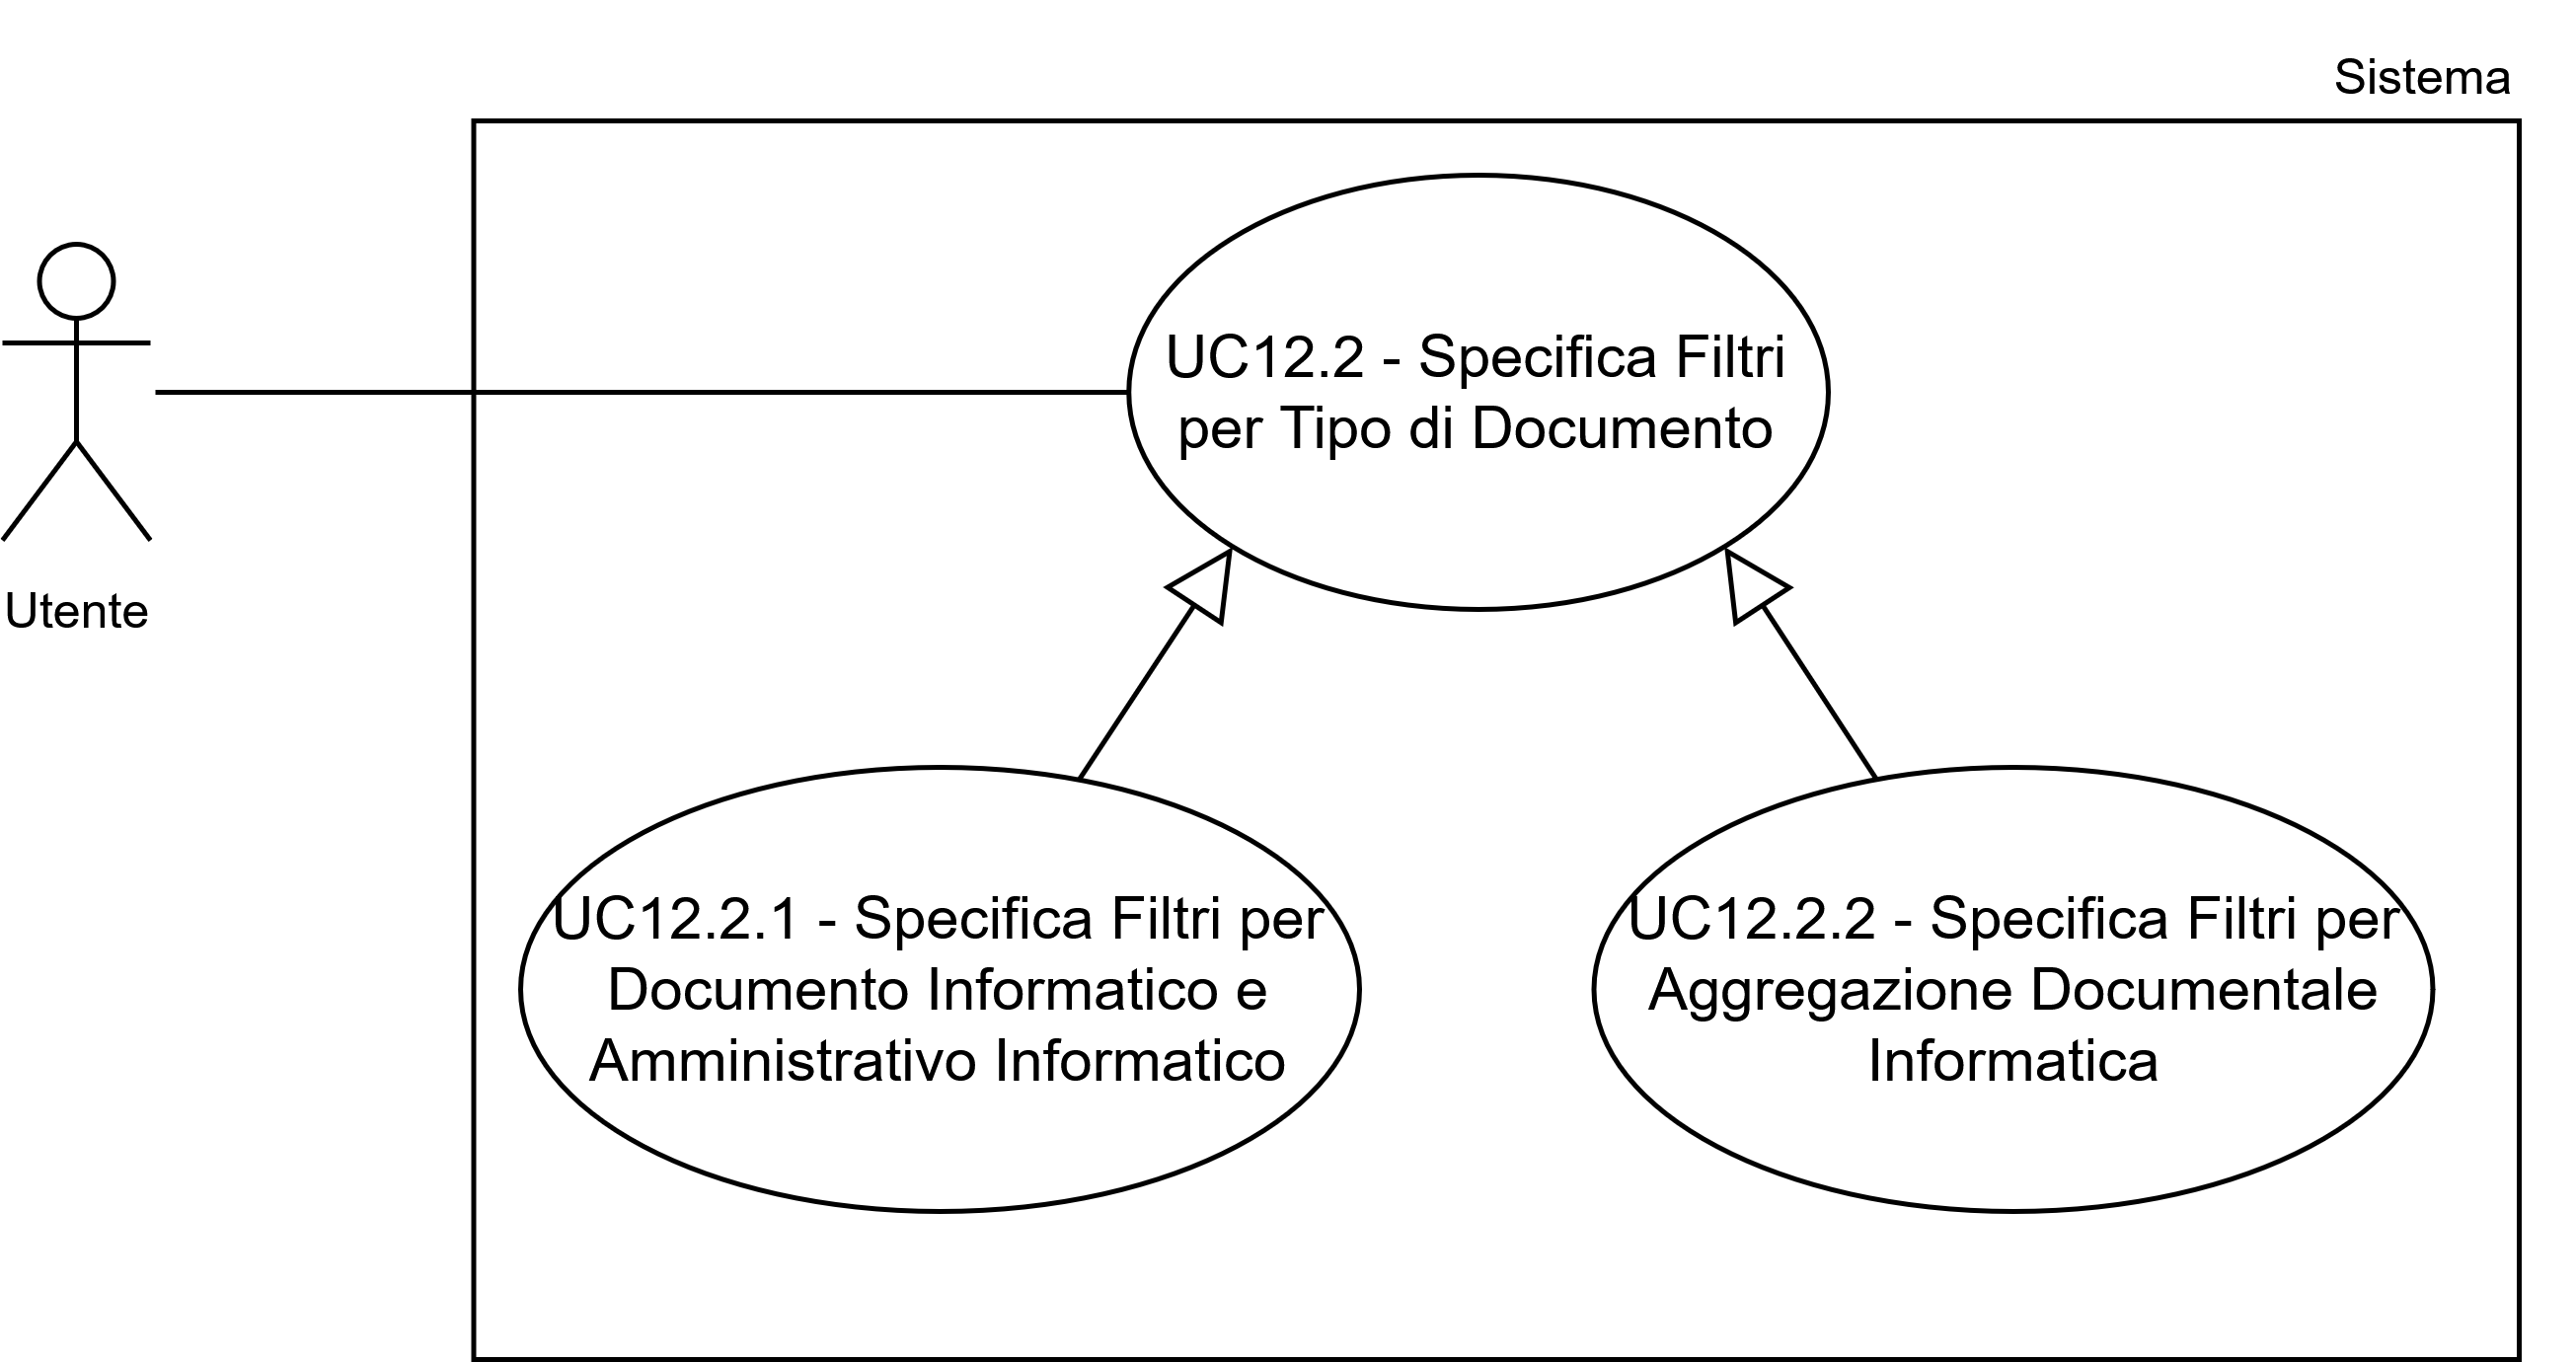
\includegraphics[width=0.9\textwidth]{../../assets/uml/UC12.2.png}
    \caption{\ref{addFiltriTipoDocumento} - Specifica filtri per Tipo di Documento}
    \label{fig:uc_specificaFiltriTipoDocumento}
\end{figure}
\begin{itemize}
      \item \textbf{Attore Primario}: Utente
      \item \textbf{Precondizioni}: 
      \begin{itemize}
            \item L'Utente ha avviato l'applicazione
            \item L'Utente sta effettuando una ricerca nel DIP con filtri
            \item L'Utente ha specificato il filtro Tipo di Documento
      \end{itemize}
      \item \textbf{Postcondizioni}: Vengono specificati i filtri per il tipo di documento selezionato e utilizzati per la generazione del risultato.
      \item \textbf{Flusso Principale}:
      \begin{enumerate}
            \item L'utente aggiunge i filtri specifici per il tipo di documento selezionato (descritti negli UC \ref{specificaFiltriDI-DAI} e \ref{specificaFiltriAggregazione})
      \end{enumerate}
\end{itemize}

\subsubusecase{specificaFiltriDI-DAI}{Specifica filtri per documento informatico e amministrativo informatico}
\begin{figure}[H]
    \centering
    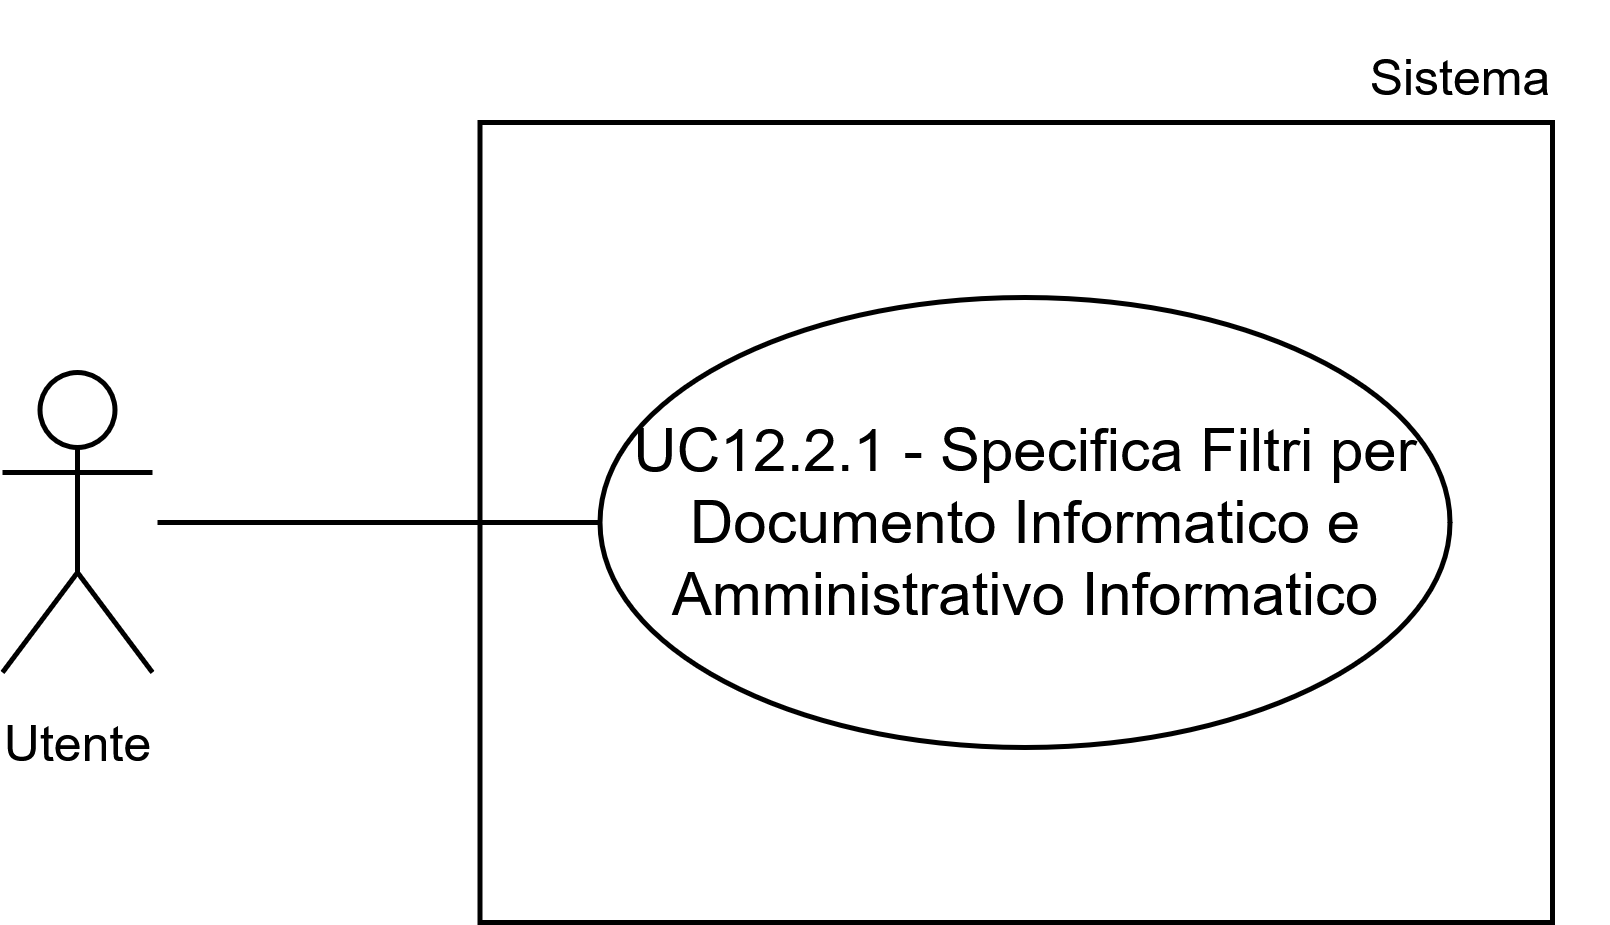
\includegraphics[width=0.6\textwidth]{../../assets/uml/UC12.2.1.png}
    \caption{\ref{specificaFiltriDI-DAI} - Specifica filtri per Documento Informatico e Amministrativo Informatico}
    \label{fig:uc_specificaFiltriDI-DAI}
\end{figure}
\begin{itemize}
      \item \textbf{Attore Primario}: Utente
      \item \textbf{Precondizioni}: 
      \begin{itemize}
            \item L'Utente ha avviato l'applicazione
            \item L'Utente sta effettuando una ricerca nel DIP con filtri
            \item L'Utente ha specificato come Tipo di Documento: Documento Informatico o Documento Amministrativo Informatico
      \end{itemize}
      \item \textbf{Postcondizioni}: Vengono specificati i filtri per i campi del Documento Informatico e Amministrativo Informatico e utilizzati per la generazione del risultato.
      \item \textbf{Flusso Principale}:
      \begin{enumerate}
            \item L'Utente seleziona i campi specifici per il tipo documento su cui basare la ricerca (\ref{selezionaCampiDI-DAI})
            \item L'Utente specifica i filtri per i campi selezionati per il tipo Documento Informatico e Amministrativo Informatico (descritti negli UC da \ref{addDatiRegistrazione} a \ref{addTracciatureModificheDocumento})
      \end{enumerate}
      \item \textbf{Inclusioni}:
      \begin{itemize}
            \item \ref{selezionaCampiDI-DAI} Seleziona campi di ricerca per \glossario{DI}/\glossario{DAI}
            \item \ref{addDatiRegistrazione} Specifica filtro \glossario{Dati di Registrazione}
            \item \ref{addTipologiaDocumentale} Specifica filtro Tipologia Documentale
            \item \ref{addModalitaFormazione} Specifica filtro \glossario{Modalità di Formazione}
            \item \ref{addRiservato} Specifica filtro campo Riservato
            \item \ref{addIdentificativoFormato} Specifica filtro \glossario{Identificativo di Formato}
            \item \ref{addDatiVerifica} Specifica filtro \glossario{Dati di Verifica}
            \item \ref{addNomeDocumento} Specifica filtro Nome del Documento
            \item \ref{addVersioneDocumento} Specifica filtro Versione del Documento
            \item \ref{addIdentificativoDocumentoPrimario} Specifica filtro Identificativo del \glossario{Documento Primario}
            \item \ref{addTracciatureModificheDocumento} Specifica filtro Tracciature di Modifiche del Documento
      \end{itemize}
      \item \textbf{Specializza}: \ref{addFiltriTipoDocumento} Specifica filtri per tipo di documento
\end{itemize}
\begin{figure}[H]
      \centering
      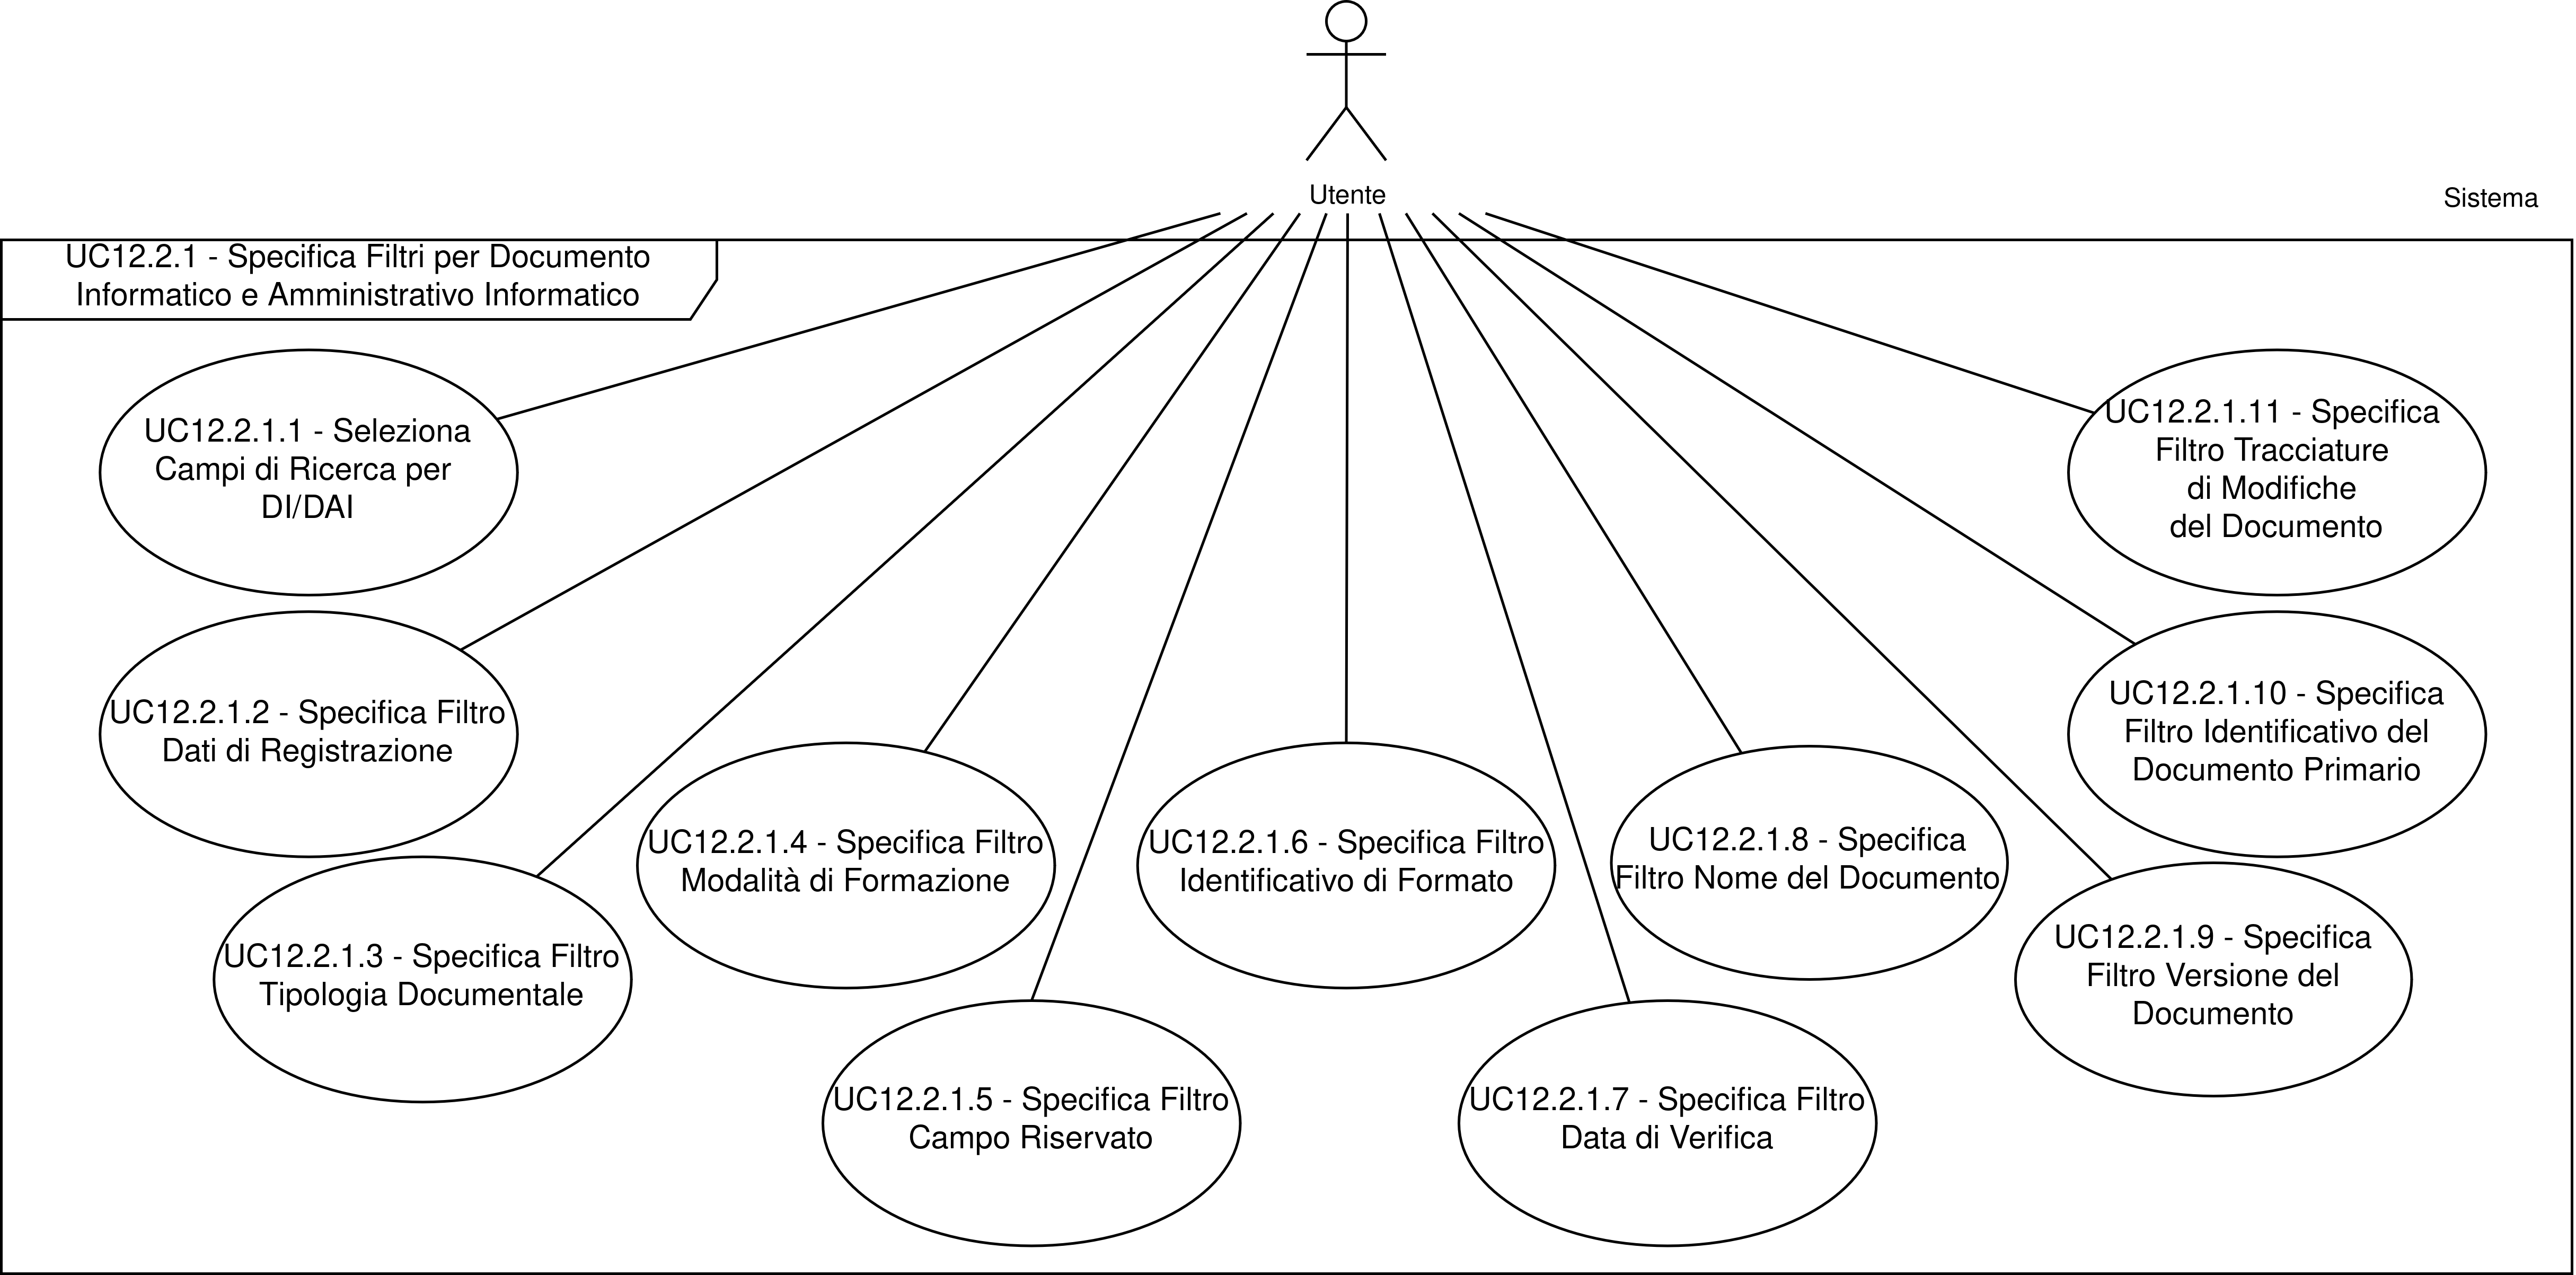
\includegraphics[width=1\textwidth]{../../assets/uml/UC12.2.1INC.png}
      \caption{Inclusioni \ref{specificaFiltriDI-DAI} - Specifica filtri per documento informatico e amministrativo informatico}
      \label{fig:inclusioniSpecificaFiltriDI-DAI}
\end{figure}

\deepusecase{selezionaCampiDI-DAI}{Selezione campi di ricerca per DI/DAI}
\begin{itemize}
      \item \textbf{Attore Primario}: Utente
      \item \textbf{Precondizioni}: \begin{itemize}
            \item L'Utente ha avviato l'applicazione
            \item L'Utente sta effettuando una ricerca nel DIP con filtri
            \item L'Utente ha selezionato il filtro per il Tipo di Documento come DI o DAI
      \end{itemize}
      \item \textbf{Postcondizioni}:  I campi selezionati dall'Utente sono aggiunti ai campi selezionati per la ricerca.
      \item \textbf{Flusso Principale}:
            \begin{enumerate}
                  \item L'Utente sceglie uno o più campi tra quelli disponibili.
                  \item Il sistema aggiunge gli elementi selezionati ai campi selezionati per la ricerca
            \end{enumerate}
\end{itemize}

\deepusecase{addDatiRegistrazione}{Specifica filtro Dati di Registrazione}
\begin{figure}[H]
      \centering
      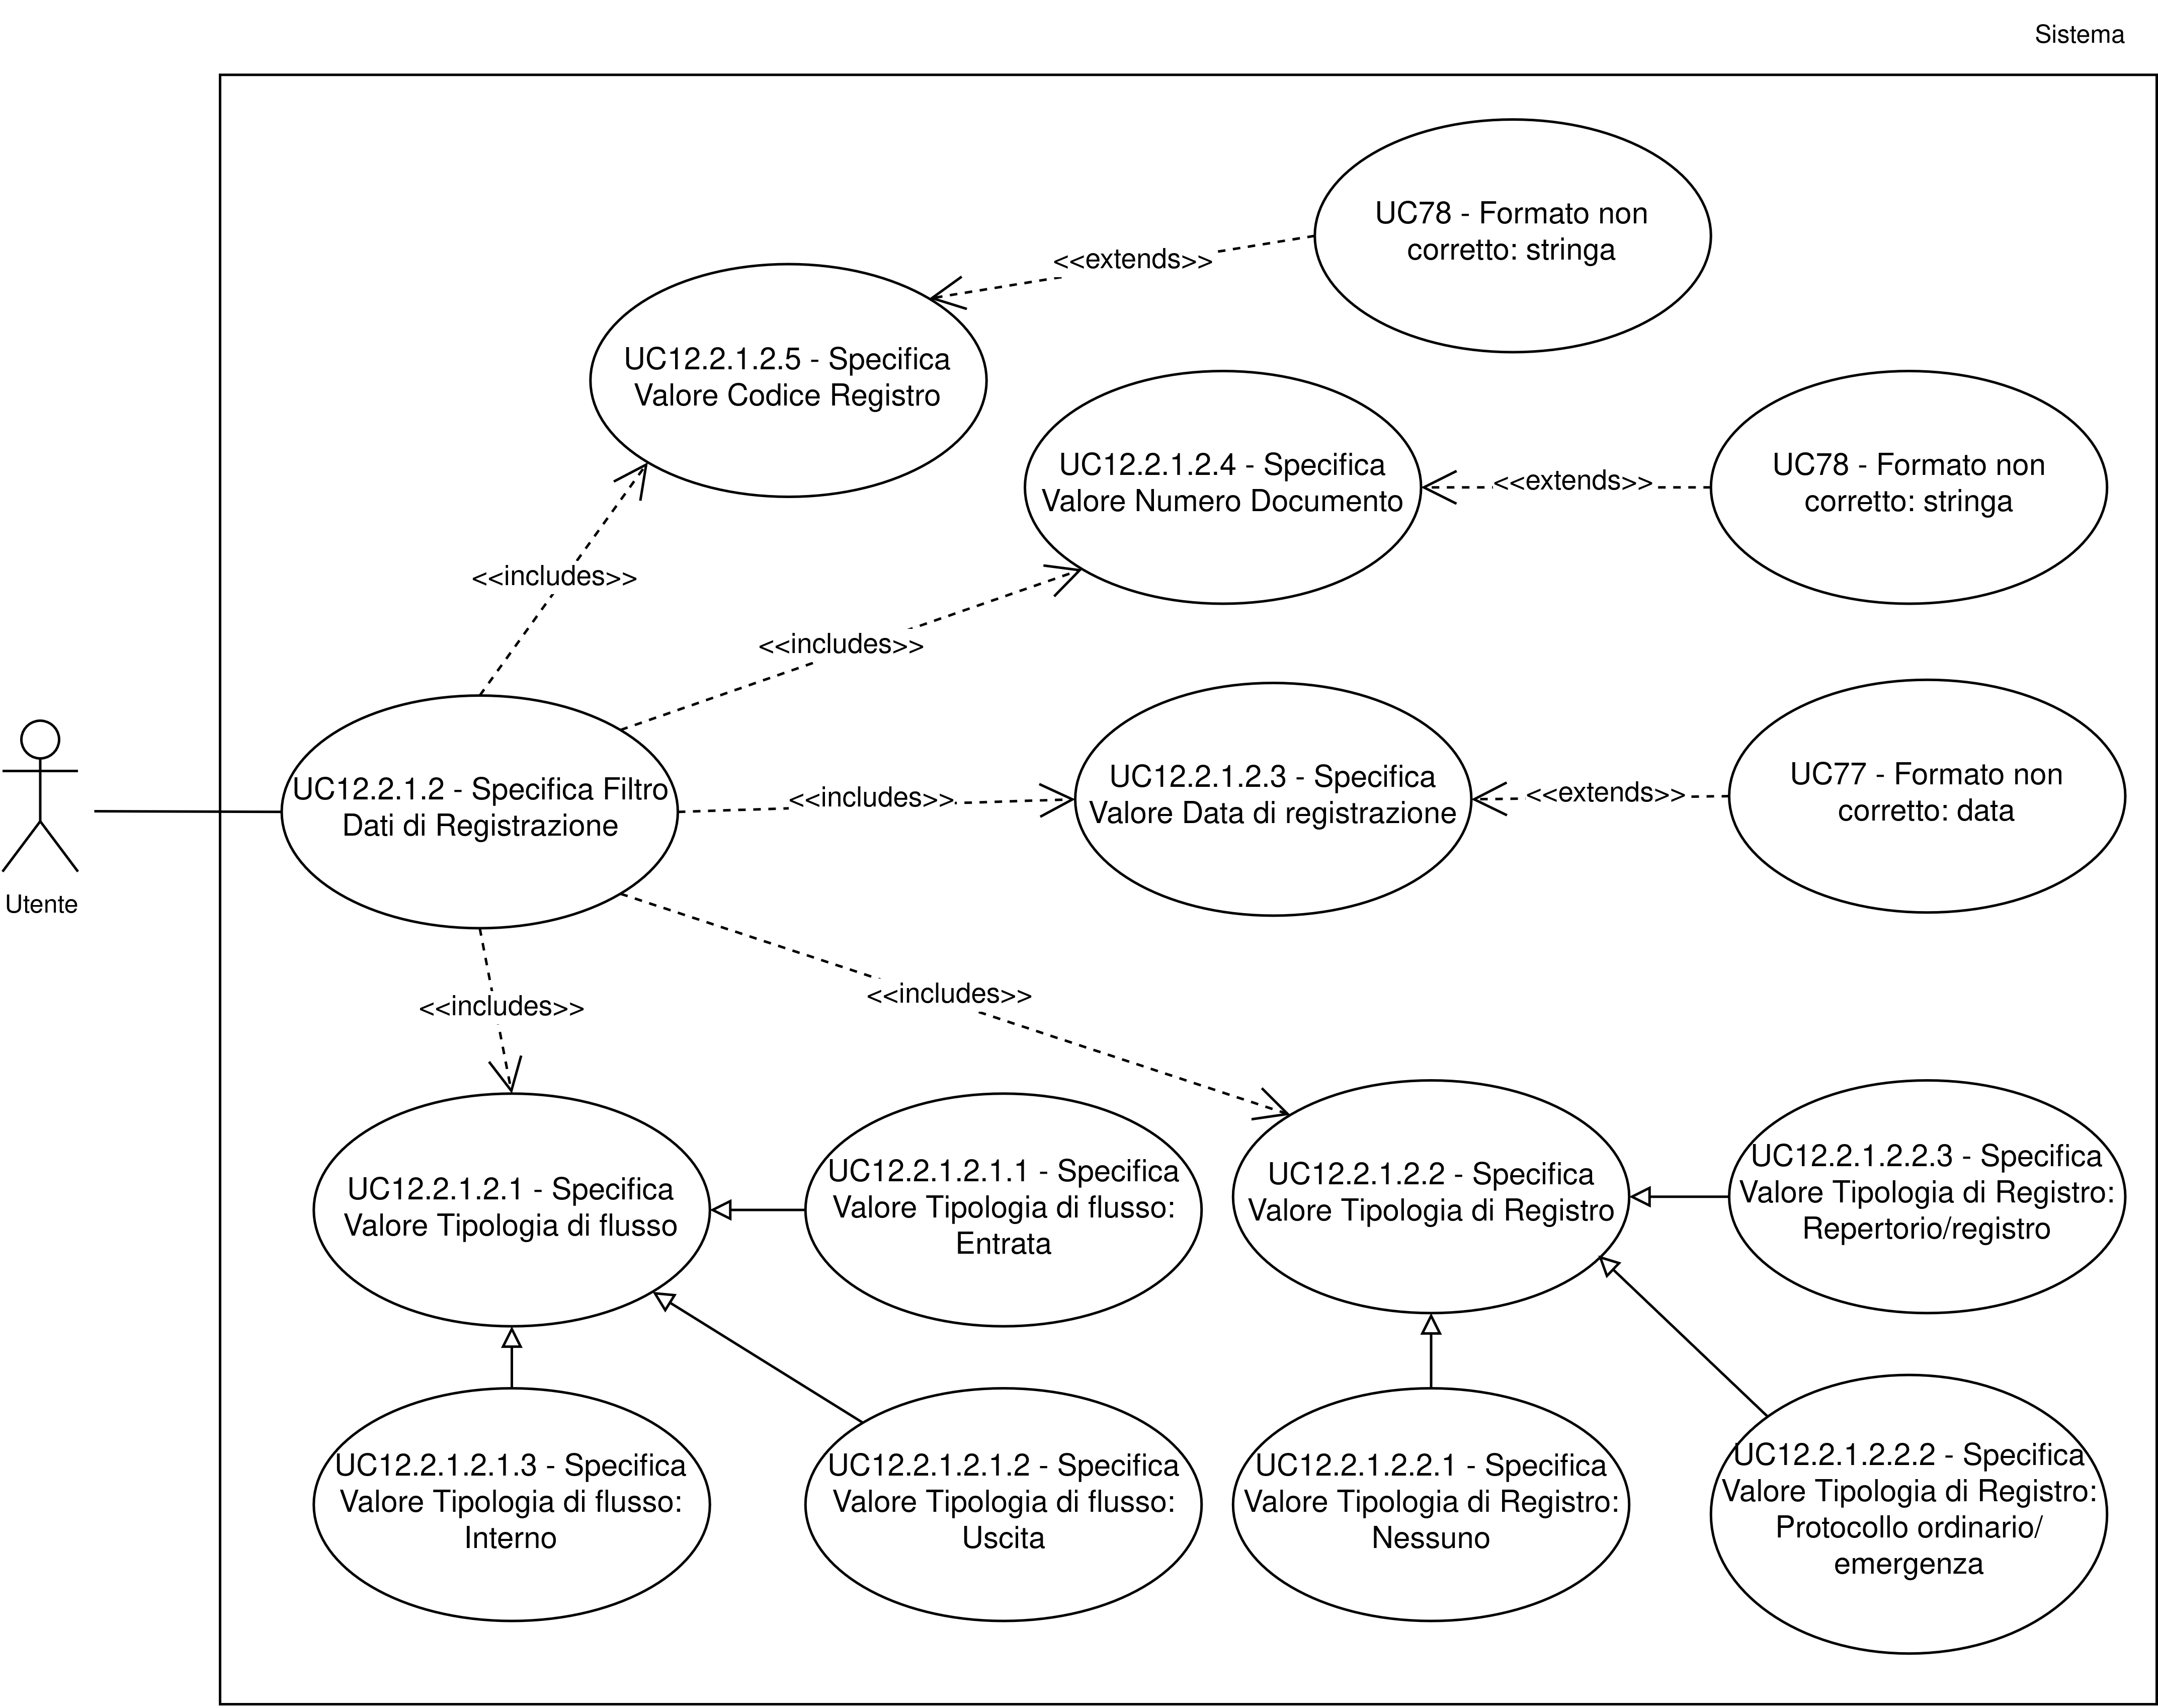
\includegraphics[width=1\textwidth]{../../assets/uml/UC12.2.1.2.png}
      \caption{Inclusioni \ref{addDatiRegistrazione} - Specifica filtro Dati di Registrazione}
      \label{fig:inclusioniSpecificaFiltriDatiRegistrazione}
\end{figure}
\begin{itemize}
      \item \textbf{Attore Primario}: Utente
      \item \textbf{Precondizioni}: 
      \begin{itemize}
            \item L'Utente ha avviato l'applicazione
            \item L'Utente sta effettuando una ricerca nel DIP con filtri
            \item L'Utente ha specificato come Tipo di Documento: Documento Informatico o Documento Amministrativo Informatico
            \item L'Utente ha selezionato il filtro Dati di Registrazione tra i campi specifici per tipo documentale
      \end{itemize}
      \item \textbf{Postcondizioni}: 
      \begin{itemize}
            \item L'Utente ha specificato i valori del filtro Dati di Registrazione
            \item Il filtro Dati di Registrazione è parametro per la ricerca con filtri e per la generazione del risultato
      \end{itemize}
      \item \textbf{Flusso Principale}:
      \begin{enumerate}
            \item L'Utente specifica la Tipologia di Flusso. (\ref{addValoreTipologiaDiFlusso})
            \item L'Utente specifica il Tipo di Registro. (\ref{addValoreTipologiaDiRegistro})
            \item L'Utente specifica la Data/Ora di Registrazione (nel caso di un documento
            protocollato tali parametri fanno riferimento alla protocollazione) 
            \item L'Utente specifica il Numero Documento (di Registrazione del Documento o di Protocollo)
            \item L'Utente specifica il Codice Registro
            \item Il sistema imposta i valori del filtro come parametri per la ricerca
      \end{enumerate}
      \item \textbf{Inclusioni}:
      \begin{itemize}
            \item \ref{addValoreTipologiaDiFlusso} Specifica valore Tipologia di Flusso
            \item \ref{addValoreTipologiaDiRegistro} Specifica valore Tipo di Registro
            \item \ref{addValoreDataRegistrazione} Specifica valore Data/Ora di Registrazione
            \item \ref{addValoreNumeroDocumento} Specifica valore Numero Documento
            \item \ref{addValoreCodiceRegistro} Specifica valore Codice Registro
      \end{itemize}
\end{itemize}


\subdeepusecase{addValoreTipologiaDiFlusso}{Specifica valore Tipologia di Flusso}\label{compilaValoreFiltroTipologiaDiFlusso}
\begin{itemize}
      \item \textbf{Attore Primario}: Utente
      \item \textbf{Precondizioni}: 
      \begin{itemize}            
            \item L'Utente ha avviato l'applicazione
            \item L'Utente sta effettuando una ricerca nel DIP con filtri
            \item L'Utente ha specificato come Tipo di Documento: Documento Informatico o Documento Amministrativo Informatico
            \item L'Utente ha selezionato il filtro Dati di Registrazione tra i campi specifici per tipo documentale
      \end{itemize}
      \item \textbf{Postcondizioni}: Il sistema riceve il valore del campo Tipologia di Flusso e lo salva per il filtro Dati di Registrazione.
      \item \textbf{Flusso Principale}:
      \begin{enumerate}
            \item L'Utente specifica la Tipologia di Flusso.
            \item Il sistema riceve il valore del campo Tipologia di Flusso e lo salva per il filtro Dati di Registrazione.
      \end{enumerate}
\end{itemize}

\subsubdeepusecase{addValoreTipologiaDiFlussoEntrata}{Specifica valore Tipologia di Flusso: Entrata}
\begin{itemize}
      \item \textbf{Attore Primario}: Utente
      \item \textbf{Precondizioni}: 
      \begin{itemize}            
            \item L'Utente ha avviato l'applicazione
            \item L'Utente sta effettuando una ricerca nel DIP con filtri
            \item L'Utente ha specificato come Tipo di Documento: Documento Informatico o Documento Amministrativo Informatico
            \item L'Utente ha selezionato il filtro Dati di Registrazione tra i campi specifici per tipo documentale
      \end{itemize}
      \item \textbf{Postcondizioni}: Il sistema riceve il valore "Entrata" per il campo Tipologia di Flusso e lo salva per il filtro Dati di Registrazione.
      \item \textbf{Flusso Principale}:
      \begin{enumerate}
            \item L'Utente specifica la Tipologia di Flusso "Entrata".
            \item Il sistema riceve il valore "Entrata" per il campo Tipologia di Flusso e lo salva per il filtro Dati di Registrazione.
      \end{enumerate}
      \item \textbf{Specializza}: \ref{addValoreTipologiaDiFlusso} Specifica valore Tipologia di Flusso
\end{itemize}

\subsubdeepusecase{addValoreTipologiaDiFlussoUscita}{Specifica valore Tipologia di Flusso: Uscita}
\begin{itemize}
      \item \textbf{Attore Primario}: Utente
      \item \textbf{Precondizioni}: 
      \begin{itemize}            
            \item L'Utente ha avviato l'applicazione
            \item L'Utente sta effettuando una ricerca nel DIP con filtri
            \item L'Utente ha specificato come Tipo di Documento: Documento Informatico o Documento Amministrativo Informatico
            \item L'Utente ha selezionato il filtro Dati di Registrazione tra i campi specifici per tipo documentale
      \end{itemize}
      \item \textbf{Postcondizioni}: Il sistema riceve il valore "Uscita" per il campo Tipologia di Flusso e lo salva per il filtro Dati di Registrazione.
      \item \textbf{Flusso Principale}:
      \begin{enumerate}
            \item L'Utente specifica la Tipologia di Flusso "Uscita".
            \item Il sistema riceve il valore "Uscita" per il campo Tipologia di Flusso e lo salva per il filtro Dati di Registrazione.
      \end{enumerate}
      \item \textbf{Specializza}: \ref{addValoreTipologiaDiFlusso} Specifica valore Tipologia di Flusso
\end{itemize}

\subsubdeepusecase{addValoreTipologiaDiFlussoInterno}{Specifica valore Tipologia di Flusso: Interno}
\begin{itemize}
      \item \textbf{Attore Primario}: Utente
      \item \textbf{Precondizioni}: 
      \begin{itemize}            
            \item L'Utente ha avviato l'applicazione
            \item L'Utente sta effettuando una ricerca nel DIP con filtri
            \item L'Utente ha specificato come Tipo di Documento: Documento Informatico o Documento Amministrativo Informatico
            \item L'Utente ha selezionato il filtro Dati di Registrazione tra i campi specifici per tipo documentale
      \end{itemize}
      \item \textbf{Postcondizioni}: Il sistema riceve il valore "Interno" per il campo Tipologia di Flusso e lo salva per il filtro Dati di Registrazione.
      \item \textbf{Flusso Principale}:
      \begin{enumerate}
            \item L'Utente specifica la Tipologia di Flusso "Interno".
            \item Il sistema riceve il valore "Interno" per il campo Tipologia di Flusso e lo salva per il filtro Dati di Registrazione.
      \end{enumerate}
      \item \textbf{Specializza}: \ref{addValoreTipologiaDiFlusso} Specifica valore Tipologia di Flusso
\end{itemize}

\subdeepusecase{addValoreTipologiaDiRegistro}{Specifica valore Tipologia di Registro}\label{compilaValoreFiltroTipologiaDiRegistro}
\begin{itemize}
      \item \textbf{Attore Primario}: Utente
      \item \textbf{Precondizioni}: 
      \begin{itemize}            
            \item L'Utente ha avviato l'applicazione
            \item L'Utente sta effettuando una ricerca nel DIP con filtri
            \item L'Utente ha specificato come Tipo di Documento: Documento Informatico o Documento Amministrativo Informatico
            \item L'Utente ha selezionato il filtro Dati di Registrazione tra i campi specifici per tipo documentale
      \end{itemize}
      \item \textbf{Postcondizioni}: Il sistema riceve il valore del campo Tipologia di Registro e lo salva per il filtro Dati di Registrazione.
      \item \textbf{Flusso Principale}:
      \begin{enumerate}
            \item L'Utente specifica la Tipologia di Registro.
            \item Il sistema riceve il valore del campo Tipologia di Registro e lo salva per il filtro Dati di Registrazione.
      \end{enumerate}
\end{itemize}

\subsubdeepusecase{addValoreTipologiaDiRegistroNessuno}{Specifica valore Tipologia di Registro: Nessuno}
\begin{itemize}
      \item \textbf{Attore Primario}: Utente
      \item \textbf{Precondizioni}: 
      \begin{itemize}            
            \item L'Utente ha avviato l'applicazione
            \item L'Utente sta effettuando una ricerca nel DIP con filtri
            \item L'Utente ha specificato come Tipo di Documento: Documento Informatico o Documento Amministrativo Informatico
            \item L'Utente ha selezionato il filtro Dati di Registrazione tra i campi specifici per tipo documentale
      \end{itemize}
      \item \textbf{Postcondizioni}: Il sistema riceve il valore "Nessuno" per il campo Tipologia di Registro e lo salva per il filtro Dati di Registrazione.
      \item \textbf{Flusso Principale}:
      \begin{enumerate}
            \item L'Utente specifica la Tipologia di Registro "Nessuno".
            \item Il sistema riceve il valore "Nessuno" per il campo Tipologia di Registro e lo salva per il filtro Dati di Registrazione.
      \end{enumerate}
      \item \textbf{Specializza}: \ref{addValoreTipologiaDiRegistro} Specifica valore Tipologia di Registro
\end{itemize}

\subsubdeepusecase{addValoreTipologiaDiRegistroProtocollo}{Specifica valore Tipologia di Registro: Protocollo Ordinario/Protocollo Emergenza}
\begin{itemize}
      \item \textbf{Attore Primario}: Utente
      \item \textbf{Precondizioni}: 
      \begin{itemize}            
            \item L'Utente ha avviato l'applicazione
            \item L'Utente sta effettuando una ricerca nel DIP con filtri
            \item L'Utente ha specificato come Tipo di Documento: Documento Informatico o Documento Amministrativo Informatico
            \item L'Utente ha selezionato il filtro Dati di Registrazione tra i campi specifici per tipo documentale
      \end{itemize}
      \item \textbf{Postcondizioni}: Il sistema riceve il valore "Protocollo Ordinario/Protocollo Emergenza" per il campo Tipologia di Registro e lo salva per il filtro Dati di Registrazione.
      \item \textbf{Flusso Principale}:
      \begin{enumerate}
            \item L'Utente specifica la Tipologia di Registro "Protocollo Ordinario/Protocollo Emergenza".
            \item Il sistema riceve il valore "Protocollo Ordinario/Protocollo Emergenza" per il campo Tipologia di Registro e lo salva per il filtro Dati di Registrazione.
      \end{enumerate}
      \item \textbf{Specializza}: \ref{addValoreTipologiaDiRegistro} Specifica valore Tipologia di Registro
\end{itemize}

\subsubdeepusecase{addValoreTipologiaDiRegistroRepertorio}{Specifica valore Tipologia di Registro: Repertorio/Registro}
\begin{itemize}
      \item \textbf{Attore Primario}: Utente
      \item \textbf{Precondizioni}: 
      \begin{itemize}            
            \item L'Utente ha avviato l'applicazione
            \item L'Utente sta effettuando una ricerca nel DIP con filtri
            \item L'Utente ha specificato come Tipo di Documento: Documento Informatico o Documento Amministrativo Informatico
            \item L'Utente ha selezionato il filtro Dati di Registrazione tra i campi specifici per tipo documentale
      \end{itemize}
      \item \textbf{Postcondizioni}: Il sistema riceve il valore "Repertorio/Registro" per il campo Tipologia di Registro e lo salva per il filtro Dati di Registrazione.
      \item \textbf{Flusso Principale}:
      \begin{enumerate}
            \item L'Utente specifica la Tipologia di Registro "Repertorio/Registro".
            \item Il sistema riceve il valore "Repertorio/Registro" per il campo Tipologia di Registro e lo salva per il filtro Dati di Registrazione.
      \end{enumerate}
      \item \textbf{Specializza}: \ref{addValoreTipologiaDiRegistro} Specifica valore Tipologia di Registro
\end{itemize}

\subdeepusecase{addValoreDataRegistrazione}{Specifica valore Data di Registrazione}
\begin{itemize}
      \item \textbf{Attore Primario}: Utente
      \item \textbf{Precondizioni}: 
      \begin{itemize}            
            \item L'Utente ha avviato l'applicazione
            \item L'Utente sta effettuando una ricerca nel DIP con filtri
            \item L'Utente ha specificato come Tipo di Documento: Documento Informatico o Documento Amministrativo Informatico
            \item L'Utente ha selezionato il filtro Dati di Registrazione tra i campi specifici per tipo documentale
      \end{itemize}
      \item \textbf{Postcondizioni}: Il sistema riceve il valore della Data di Registrazione e lo salva per il filtro Dati di Registrazione.
      \item \textbf{Flusso Principale}:
      \begin{enumerate}
            \item L'Utente specifica la Data di Registrazione.
            \item Il sistema riceve il valore della Data di Registrazione e lo salva per il filtro Dati di Registrazione.
      \end{enumerate}
      \item \textbf{Flusso Alternativo}:
      \begin{itemize}
            \item L'Utente inserisce una data non valida per il filtro Data di Registrazione (\ref{formatoNonCorrettoData})
      \end{itemize}
      \item \textbf{Estensioni}: \ref{formatoNonCorrettoData} Formato non corretto: data
\end{itemize}

\subdeepusecase{addValoreNumeroDocumento}{Specifica valore Numero Documento}
\begin{itemize}
      \item \textbf{Attore Primario}: Utente
      \item \textbf{Precondizioni}: 
      \begin{itemize}            
            \item L'Utente ha avviato l'applicazione
            \item L'Utente sta effettuando una ricerca nel DIP con filtri
            \item L'Utente ha specificato come Tipo di Documento: Documento Informatico o Documento Amministrativo Informatico
            \item L'Utente ha selezionato il filtro Dati di Registrazione tra i campi specifici per tipo documentale
      \end{itemize}
      \item \textbf{Postcondizioni}: Il sistema riceve il valore del Numero Documento e lo salva per il filtro Dati di Registrazione.
      \item \textbf{Flusso Principale}:
      \begin{enumerate}
            \item L'Utente specifica il Numero Documento.
            \item Il sistema riceve il valore del Numero Documento e lo salva per il filtro Dati di Registrazione.
      \end{enumerate}
      \item \textbf{Flusso Alternativo}:
      \begin{itemize}
            \item L'Utente inserisce un numero non valido per il filtro Numero Documento (\ref{formatoNonCorrettoStringa})
      \end{itemize}
      \item \textbf{Estensioni}: \ref{formatoNonCorrettoStringa} Formato non corretto: stringa
\end{itemize}

\subdeepusecase{addValoreCodiceRegistro}{Specifica valore Codice Registro}
\begin{itemize}
      \item \textbf{Attore Primario}: Utente
      \item \textbf{Precondizioni}: 
      \begin{itemize}            
            \item L'Utente ha avviato l'applicazione
            \item L'Utente sta effettuando una ricerca nel DIP con filtri
            \item L'Utente ha specificato come Tipo di Documento: Documento Informatico o Documento Amministrativo Informatico
            \item L'Utente ha selezionato il filtro Dati di Registrazione tra i campi specifici per tipo documentale
      \end{itemize}
      \item \textbf{Postcondizioni}: Il sistema riceve il valore del Codice Registro e lo salva per il filtro Dati di Registrazione.
      \item \textbf{Flusso Principale}:
      \begin{enumerate}
            \item L'Utente specifica il Codice Registro.
            \item Il sistema riceve il valore del Codice Registro e lo salva per il filtro Dati di Registrazione.
      \end{enumerate}
      \item \textbf{Flusso Alternativo}:
      \begin{itemize}
            \item L'Utente inserisce un codice non valido per il filtro Codice Registro (\ref{formatoNonCorrettoStringa})
      \end{itemize}
      \item \textbf{Estensioni}: \ref{formatoNonCorrettoStringa} Formato non corretto: stringa
\end{itemize}

\deepusecase{addTipologiaDocumentale}{Specifica filtro Tipologia Documentale}
\begin{figure}[H]
      \centering
      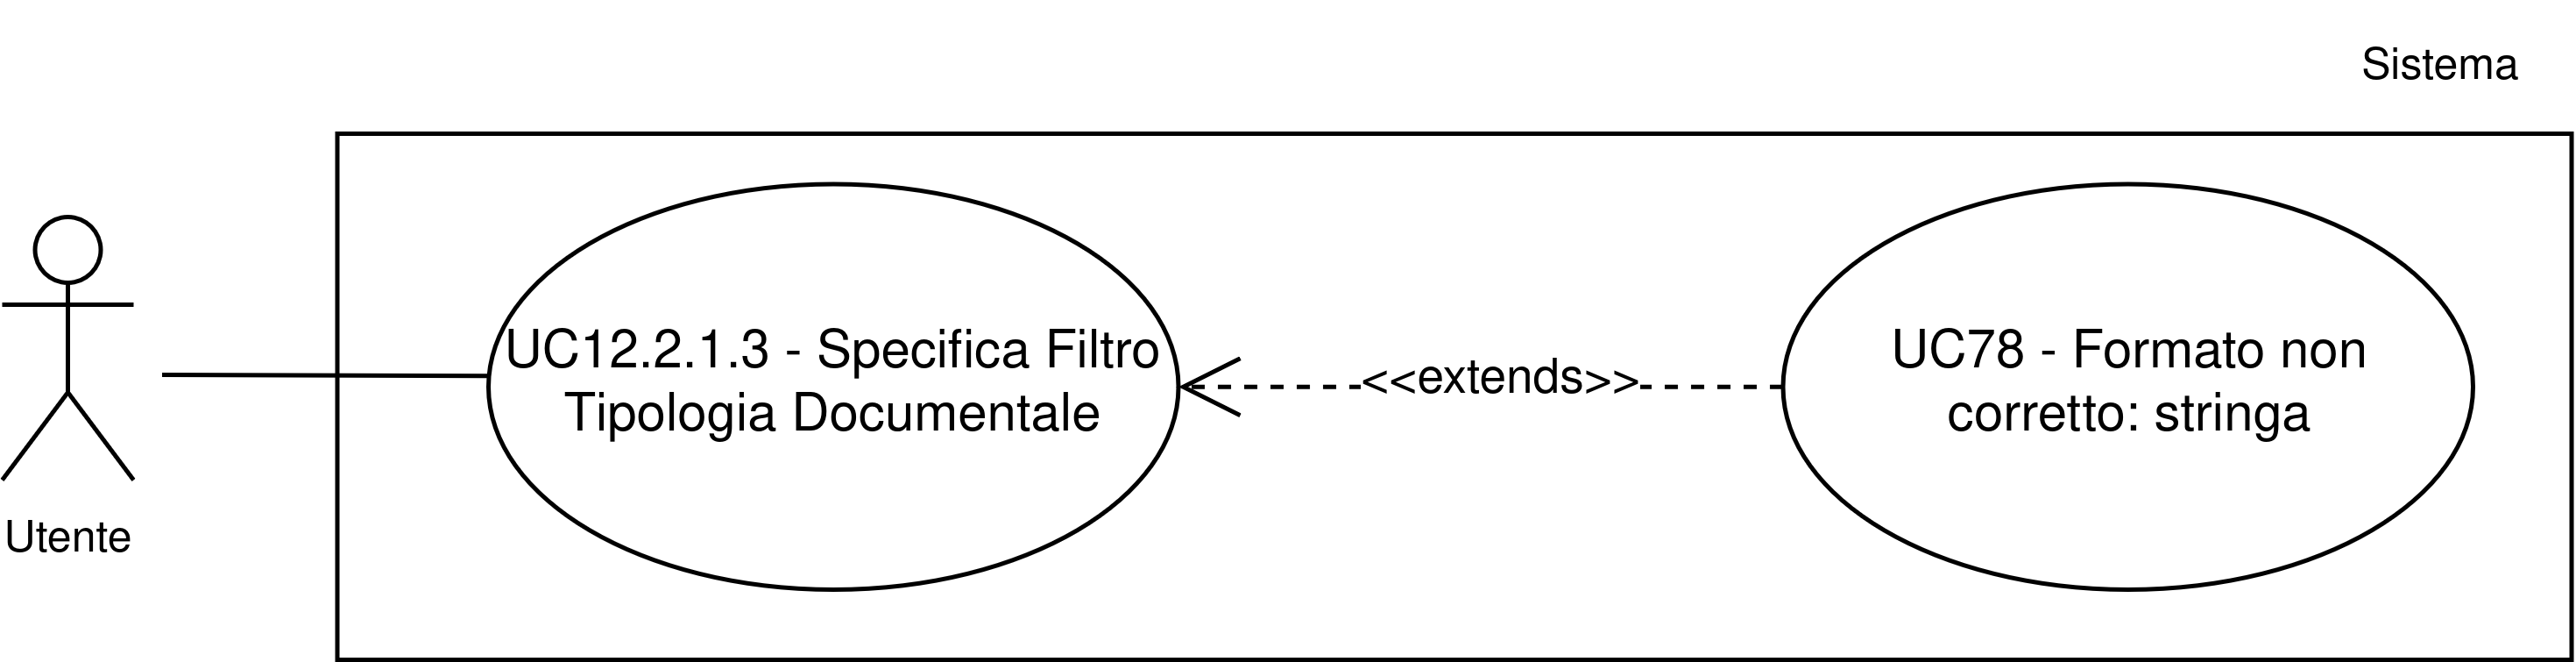
\includegraphics[width=1\textwidth]{../../assets/uml/UC12.2.1.3.png}
      \caption{Inclusioni \ref{addTipologiaDocumentale} - Specifica filtro Tipologia Documentale}
      \label{fig:inclusioniSpecificaFiltriTipologiaDocumentale}
\end{figure}
\begin{itemize}
      \item \textbf{Attore Primario}: Utente
      \item \textbf{Precondizioni}: 
      \begin{itemize}
            \item L'Utente ha avviato l'applicazione
            \item L'Utente sta effettuando una ricerca nel DIP con filtri
            \item L'Utente ha specificato come tipo di documento: Documento Informatico o Documento Amministrativo Informatico
            \item L'utente ha selezionato il filtro Tipologia Documentale tra i campi specifici per tipo documentale
      \end{itemize}
      \item \textbf{Postcondizioni}: 
      \begin{itemize}
            \item L'Utente ha specificato i valori del filtro Tipologia Documentale
            \item Il filtro Tipologia Documentale è parametro per la ricerca con filtri e per la generazione del risultato
      \end{itemize}
      \item \textbf{Flusso Principale}:
      \begin{enumerate}
            \item L'Utente specifica il nome della Tipologia Documentale (fatture, delibere,
            determine,...)
            \item Il sistema imposta questo valore come parametro per la ricerca
      \end{enumerate}
      \item \textbf{Flusso Alternativo}:
      \begin{itemize}
            \item L'Utente inserisce un nome non valido per il filtro Tipologia Documentale (\ref{formatoNonCorrettoStringa})
      \end{itemize}
      \item \textbf{Estensioni}: \ref{formatoNonCorrettoStringa} Formato non corretto: stringa
\end{itemize}

\deepusecase{addModalitaFormazione}{Specifica filtro Modalità di Formazione}
\begin{figure}[H]
      \centering
      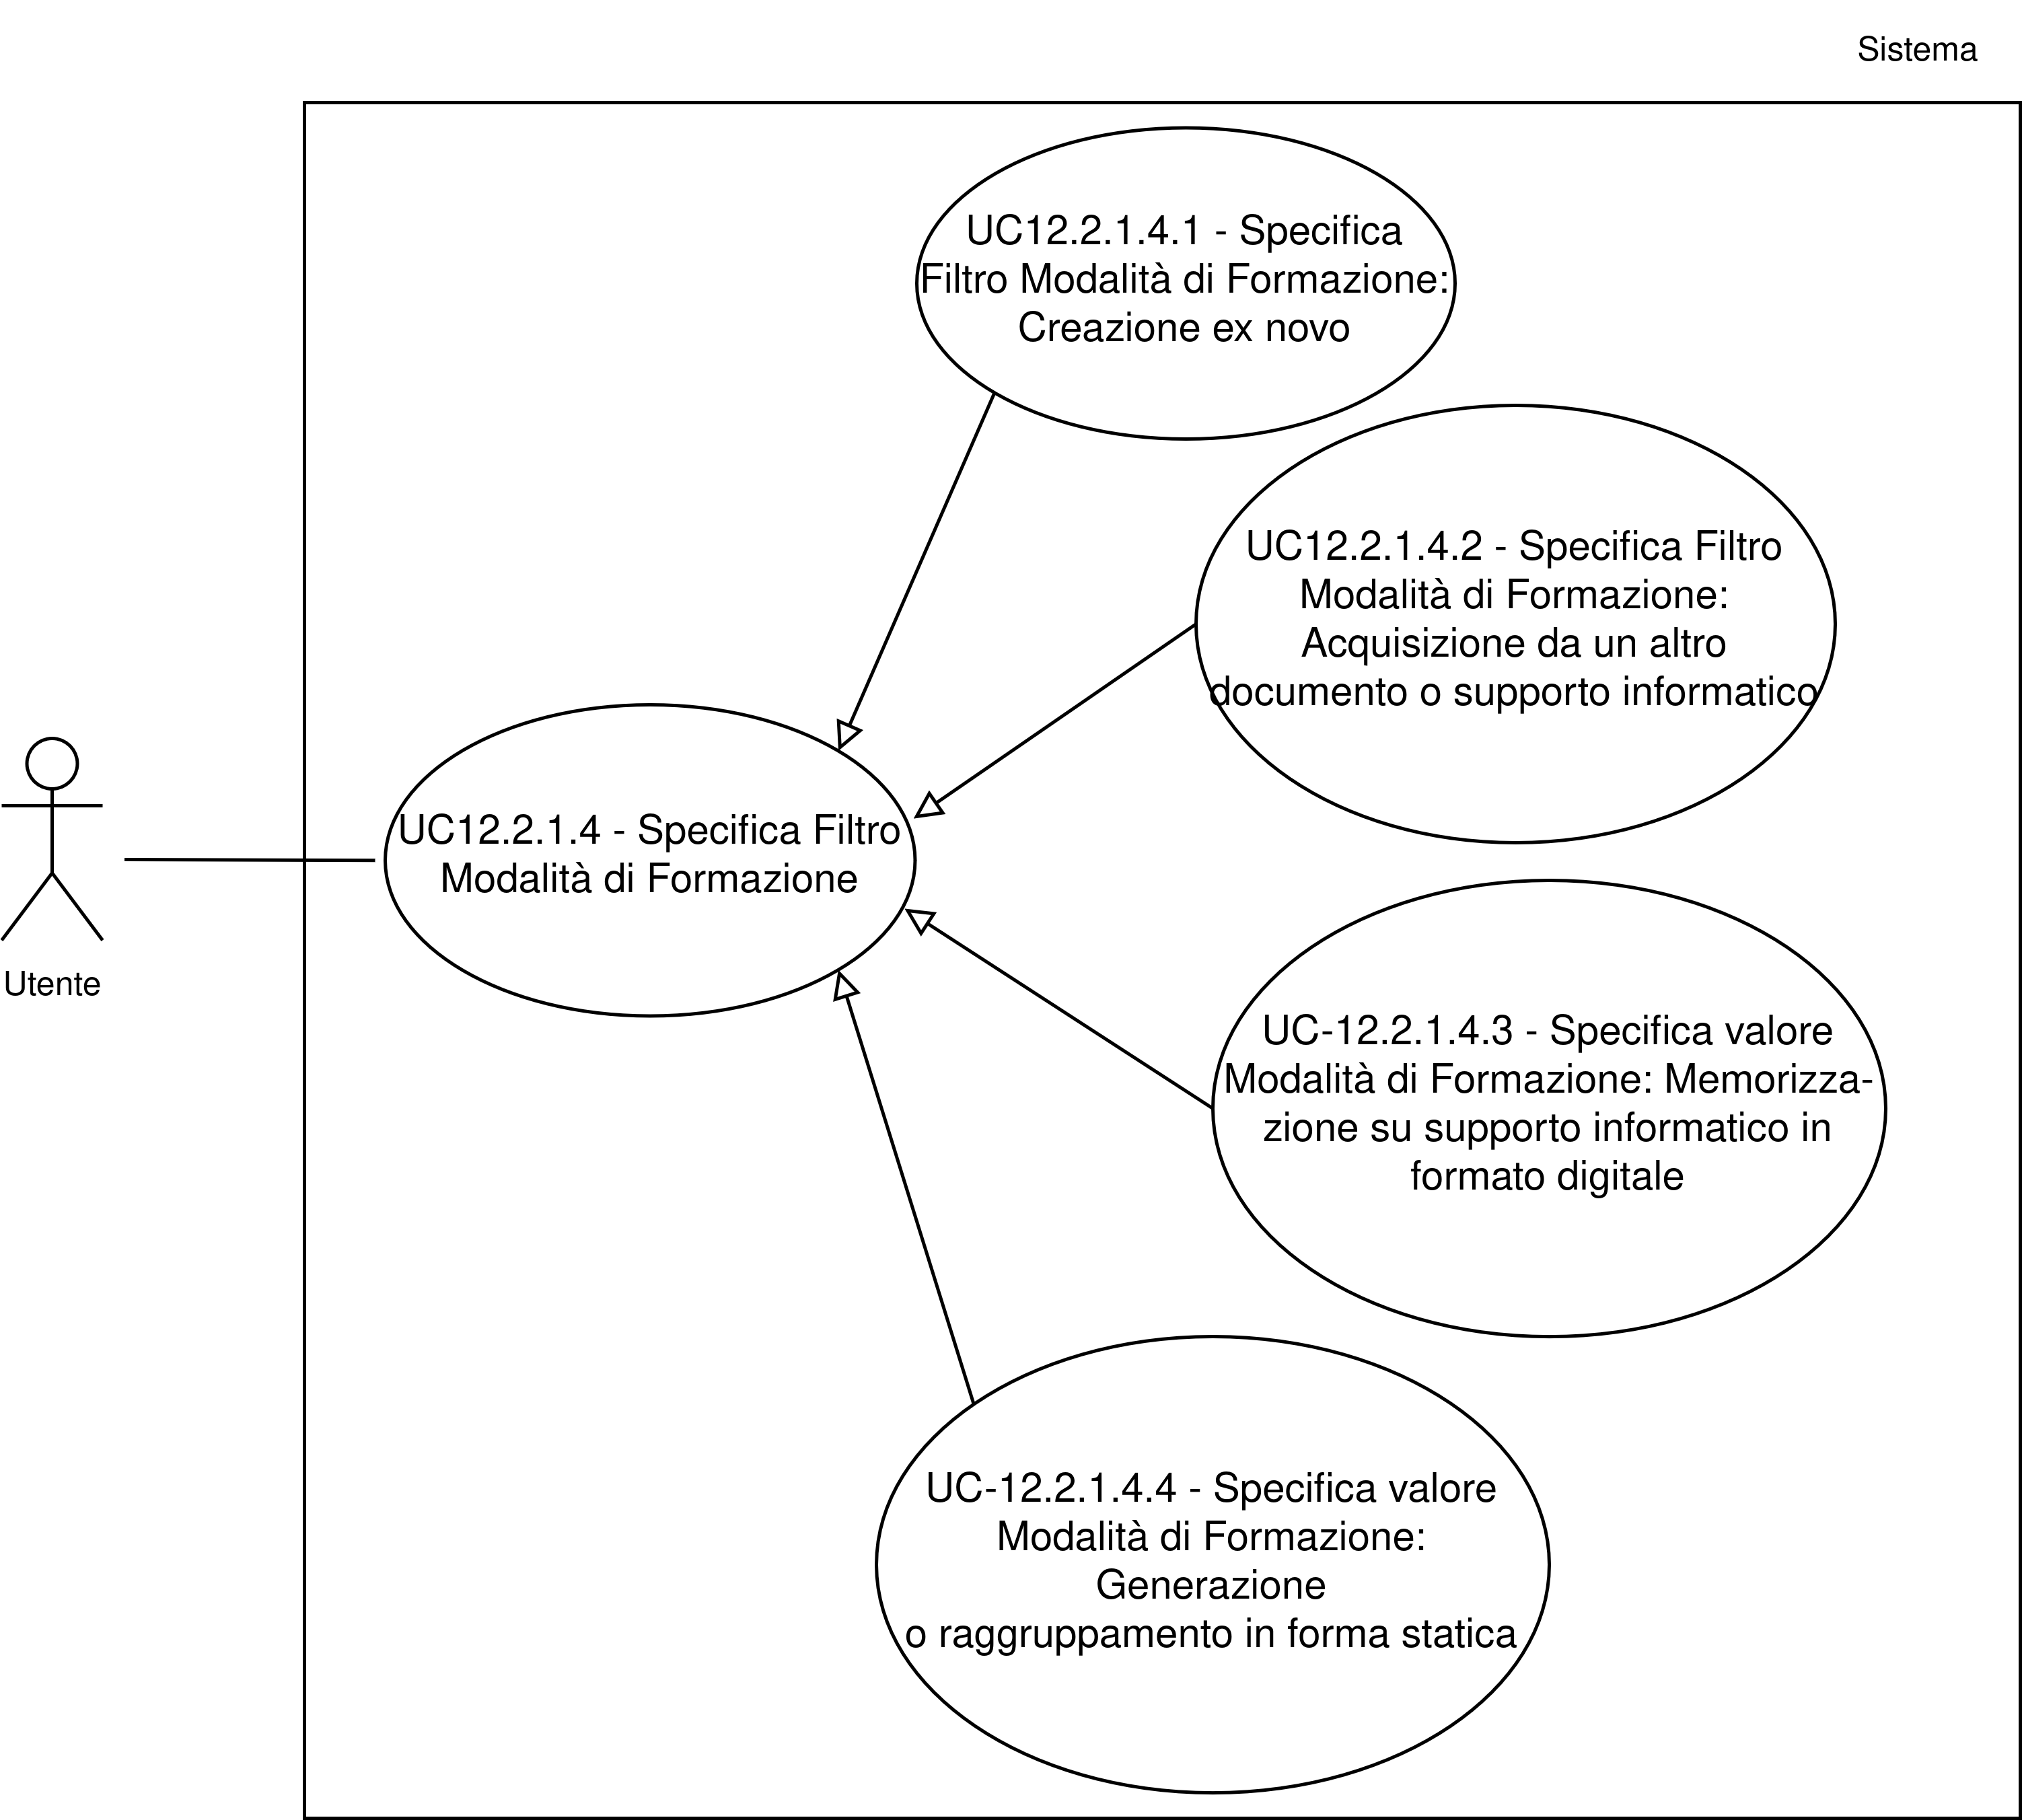
\includegraphics[width=1\textwidth]{../../assets/uml/UC12.2.1.4.png}
      \caption{Inclusioni \ref{addModalitaFormazione} - Specifica filtro Modalità di Formazione}
      \label{fig:inclusioniSpecificaFiltriModalitaFormazione}
\end{figure}
\begin{itemize}
      \item \textbf{Attore Primario}: Utente
      \item \textbf{Precondizioni}: 
      \begin{itemize}
            \item L'Utente ha avviato l'applicazione
            \item L'Utente sta effettuando una ricerca nel DIP con filtri
            \item L'Utente ha specificato come tipo di documento: Documento Informatico o Documento Amministrativo Informatico
            \item L'utente ha selezionato il filtro Modalità di Formazione tra i campi specifici per tipo documentale
      \end{itemize}
      \item \textbf{Postcondizioni}: 
      \begin{itemize}
            \item L'Utente ha specificato i valori del filtro Modalità di Formazione
            \item Il filtro Modalità di Formazione è parametro per la ricerca con filtri e per la generazione del risultato
      \end{itemize}
      \item \textbf{Flusso Principale}:
      \begin{enumerate}
            \item L'Utente specifica la Modalità di Formazione.
            \item Il sistema imposta questo valore come parametro per la ricerca
      \end{enumerate}
\end{itemize}

\subdeepusecase{addModalitaFormazioneExNovo}{Specifica valore Modalità di Formazione: Creazione ex novo}
\begin{itemize}
      \item \textbf{Attore Primario}: Utente
      \item \textbf{Precondizioni}: 
      \begin{itemize}
            \item L'Utente ha avviato l'applicazione
            \item L'Utente sta effettuando una ricerca nel DIP con filtri
            \item L'Utente ha specificato come tipo di documento: Documento Informatico o Documento Amministrativo Informatico
            \item L'utente ha selezionato il filtro Modalità di Formazione tra i campi specifici per tipo documentale
      \end{itemize}
      \item \textbf{Postcondizioni}: Il sistema riceve il valore "Creazione di un documento informatico ex novo" per il filtro Modalità di Formazione ed è parametro per la ricerca.
      \item \textbf{Flusso Principale}:
      \begin{enumerate}
            \item L'Utente specifica la Modalità di Formazione "Creazione di un documento informatico ex novo".
            \item Il sistema riceve il valore "Creazione di un documento informatico ex novo" per il filtro Modalità di Formazione e lo imposta come parametro per la ricerca.
      \end{enumerate}
      \item \textbf{Specializza}: \ref{addModalitaFormazione}
\end{itemize}

\subdeepusecase{addModalitaFormazioneAcquisizione}{Specifica valore Modalità di Formazione: Acquisizione da altro documento o supporto informatico}
\begin{itemize}
      \item \textbf{Attore Primario}: Utente
      \item \textbf{Precondizioni}: 
      \begin{itemize}
            \item L'Utente ha avviato l'applicazione
            \item L'Utente sta effettuando una ricerca nel DIP con filtri
            \item L'Utente ha specificato come tipo di documento: Documento Informatico o Documento Amministrativo Informatico
            \item L'utente ha selezionato il filtro Modalità di Formazione tra i campi specifici per tipo documentale
      \end{itemize}
      \item \textbf{Postcondizioni}: Il sistema riceve il valore "Acquisizione di un documento informatico da altro documento informatico o da supporto informatico" per il filtro Modalità di Formazione ed è parametro per la ricerca.
      \item \textbf{Flusso Principale}:
      \begin{enumerate}
            \item L'Utente specifica la Modalità di Formazione "Acquisizione di un documento informatico da altro documento informatico o da supporto informatico".
            \item Il sistema riceve il valore "Acquisizione di un documento informatico da altro documento informatico o da supporto informatico" per il filtro Modalità di Formazione e lo imposta come parametro per la ricerca.
      \end{enumerate}
      \item \textbf{Specializza}: \ref{addModalitaFormazione}
\end{itemize}

\subdeepusecase{addModalitaFormazioneMemorizzazione}{Specifica valore Modalità di Formazione: Memorizzazione su supporto informatico in formato digitale}
\begin{itemize}
      \item \textbf{Attore Primario}: Utente
      \item \textbf{Precondizioni}: 
      \begin{itemize}
            \item L'Utente ha avviato l'applicazione
            \item L'Utente sta effettuando una ricerca nel DIP con filtri
            \item L'Utente ha specificato come tipo di documento: Documento Informatico o Documento Amministrativo Informatico
            \item L'utente ha selezionato il filtro Modalità di Formazione tra i campi specifici per tipo documentale
      \end{itemize}
      \item \textbf{Postcondizioni}: Il sistema riceve il valore "Memorizzazione su supporto informatico in formato digitale" per il filtro Modalità di Formazione ed è parametro per la ricerca.
      \item \textbf{Flusso Principale}:
      \begin{enumerate}
            \item L'Utente specifica la Modalità di Formazione "Memorizzazione su supporto informatico in formato digitale".
            \item Il sistema riceve il valore "Memorizzazione su supporto informatico in formato digitale" per il filtro Modalità di Formazione e lo imposta come parametro per la ricerca.
      \end{enumerate}
      \item \textbf{Specializza}: \ref{addModalitaFormazione}
\end{itemize}

\subdeepusecase{addModalitaFormazioneGenerazione}{Specifica valore Modalità di Formazione: Generazione o raggruppamento in forma statica}
\begin{itemize}
      \item \textbf{Attore Primario}: Utente
      \item \textbf{Precondizioni}: 
      \begin{itemize}
            \item L'Utente ha avviato l'applicazione
            \item L'Utente sta effettuando una ricerca nel DIP con filtri
            \item L'Utente ha specificato come tipo di documento: Documento Informatico o Documento Amministrativo Informatico
            \item L'utente ha selezionato il filtro Modalità di Formazione tra i campi specifici per tipo documentale
      \end{itemize}
      \item \textbf{Postcondizioni}: Il sistema riceve il valore "Generazione o raggruppamento in forma statica" per il filtro Modalità di Formazione ed è parametro per la ricerca.
      \item \textbf{Flusso Principale}:
      \begin{enumerate}
            \item L'Utente specifica la Modalità di Formazione "Generazione o raggruppamento in forma statica".
            \item Il sistema riceve il valore "Generazione o raggruppamento in forma statica" per il filtro Modalità di Formazione e lo imposta come parametro per la ricerca.
      \end{enumerate}
      \item \textbf{Specializza}: \ref{addModalitaFormazione}
\end{itemize}

\deepusecase{addRiservato}{Specifica filtro campo Riservato}
\begin{itemize}
      \item \textbf{Attore Primario}: Utente
      \item \textbf{Precondizioni}: 
      \begin{itemize}
            \item L'Utente ha avviato l'applicazione
            \item L'Utente sta effettuando una ricerca nel DIP con filtri
            \item L'Utente ha specificato come tipo di documento: Documento Informatico o Documento Amministrativo Informatico
            \item L'utente ha selezionato il filtro Riservato tra i campi specifici per tipo documentale
      \end{itemize}
      \item \textbf{Postcondizioni}: 
      \begin{itemize}
            \item L'Utente ha specificato i valori del filtro Riservato
            \item Il filtro Riservato è parametro per la ricerca con filtri e per la generazione del risultato
      \end{itemize}
      \item \textbf{Flusso Principale}:
      \begin{enumerate}
            \item L'Utente specifica se il file è Riservato o meno (si/no).
            \item Il sistema imposta questo valore come parametro per la ricerca.
      \end{enumerate}
\end{itemize}

\deepusecase{addIdentificativoFormato}{Specifica filtro Identificativo di Formato}
\begin{figure}[H]
      \centering
      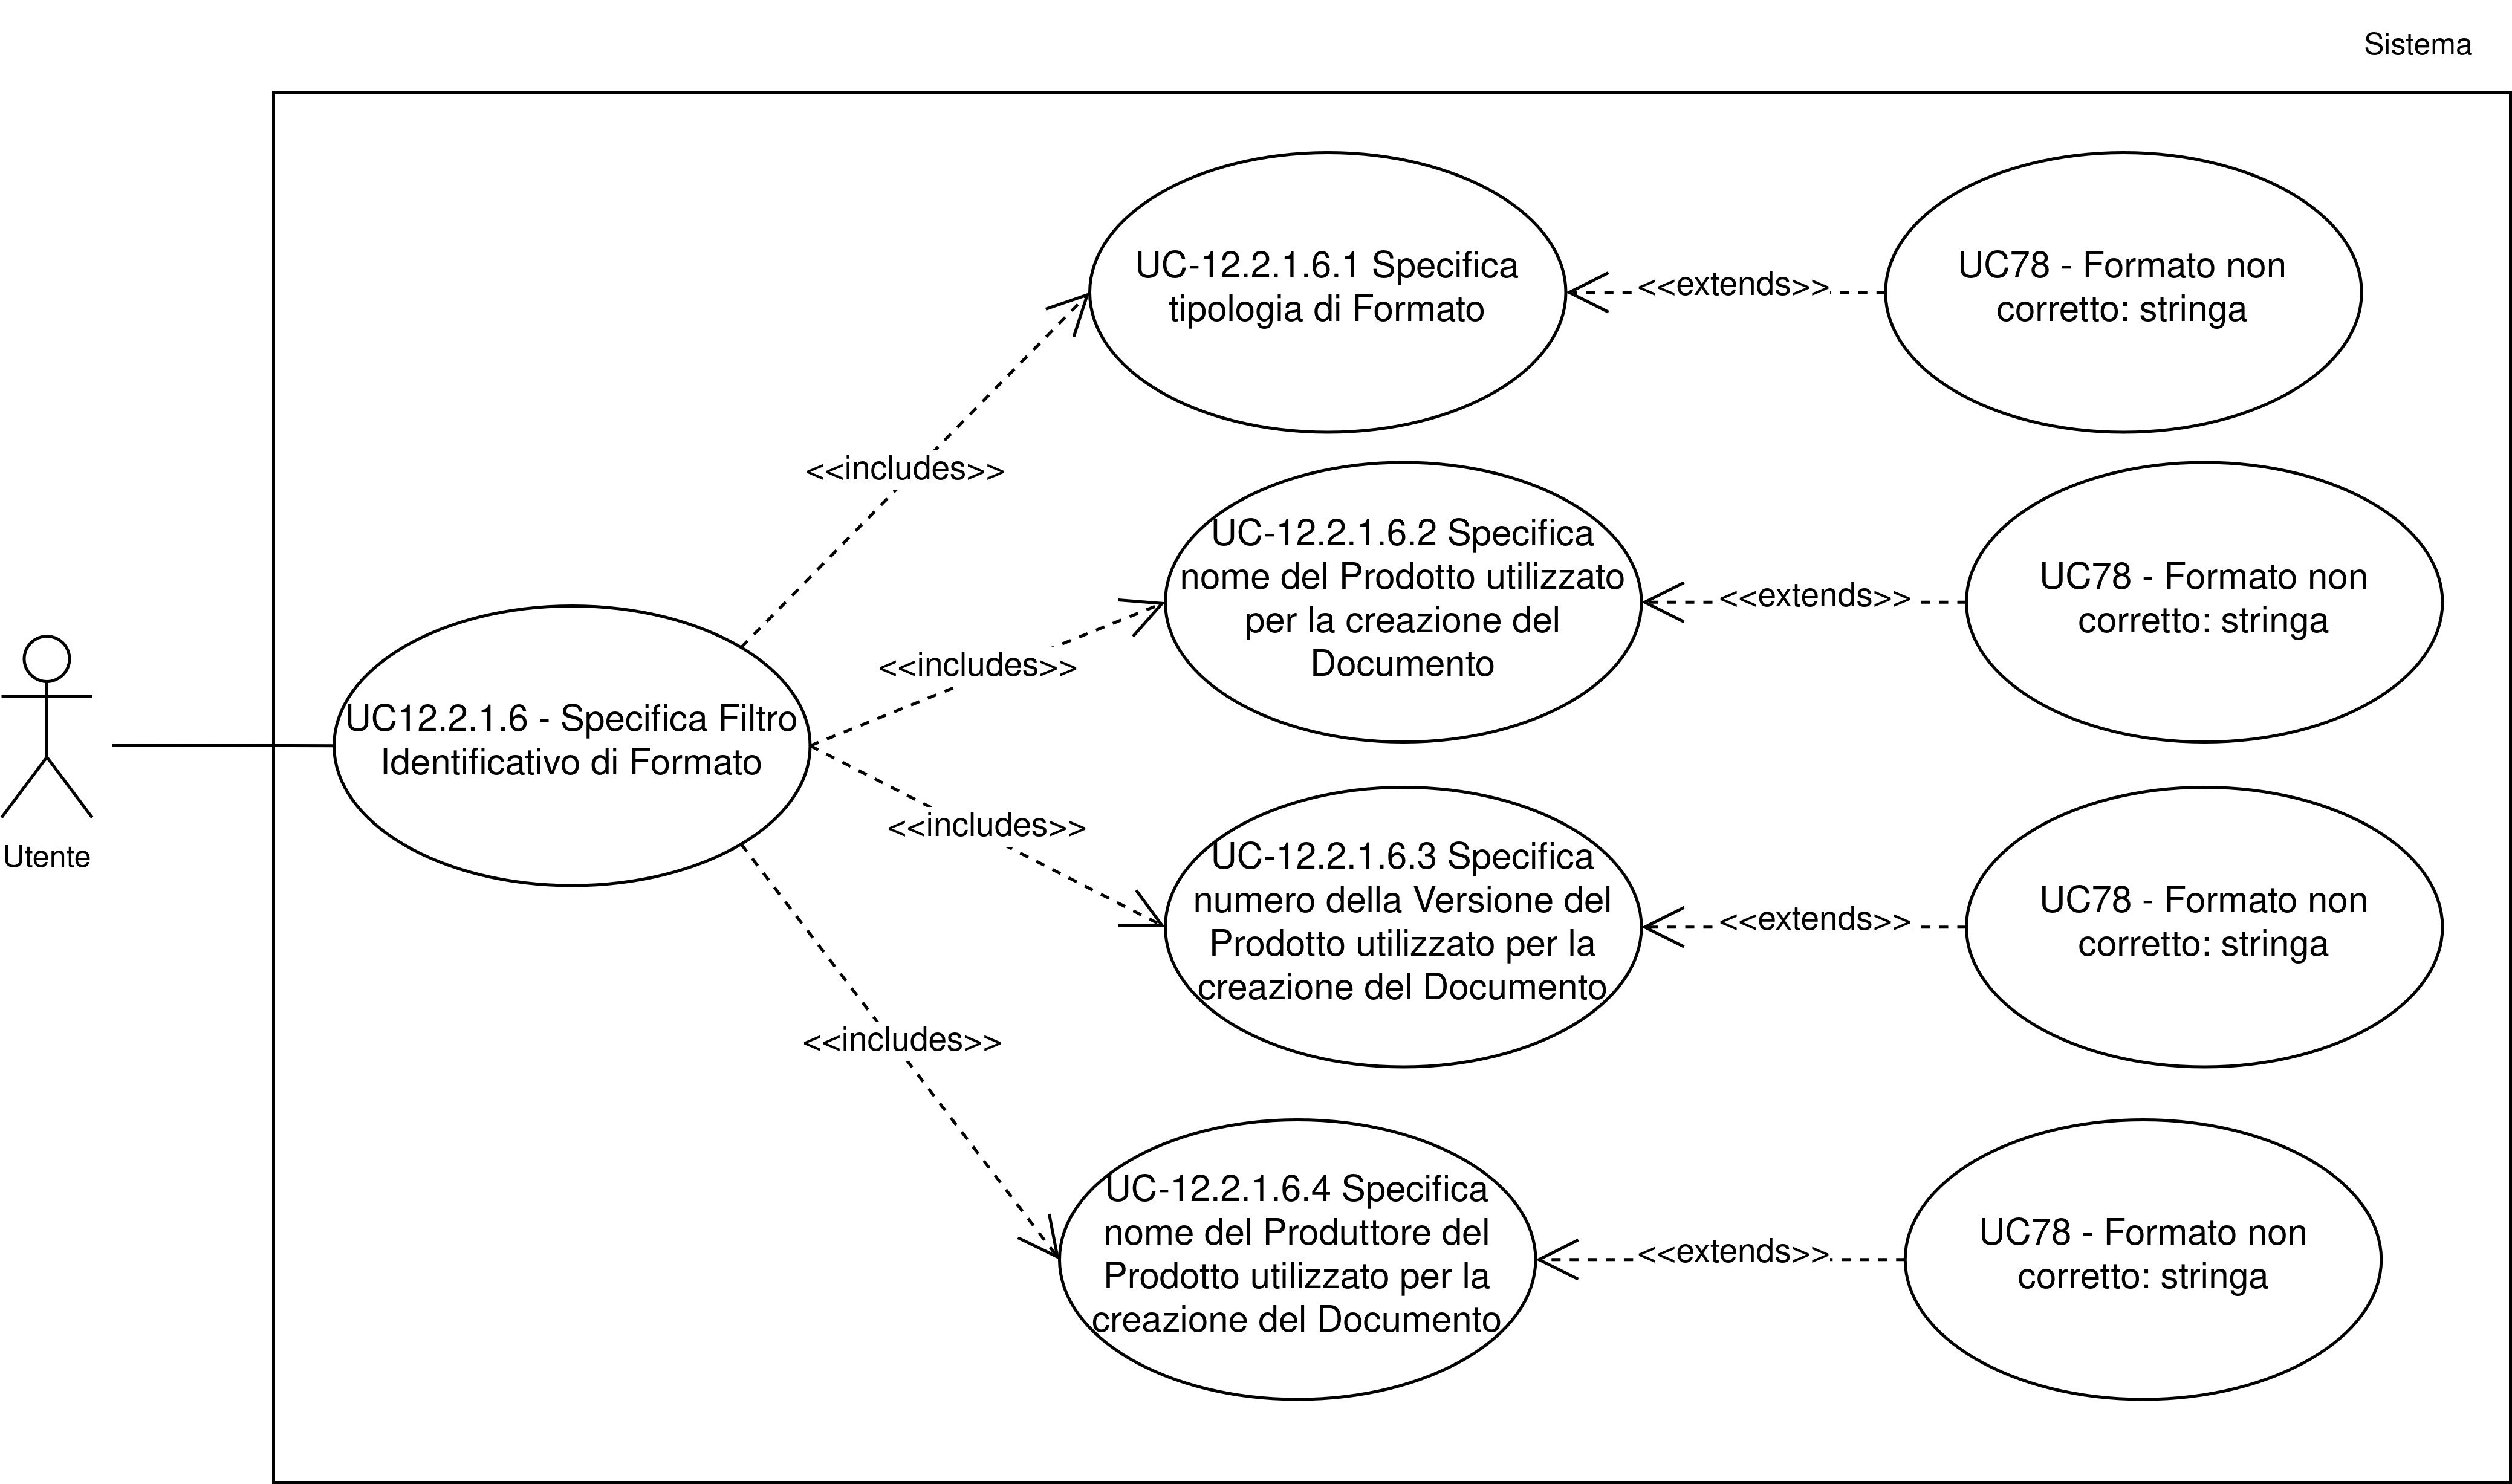
\includegraphics[width=1\textwidth]{../../assets/uml/UC12.2.1.6.png}
      \caption{Inclusioni \ref{addIdentificativoFormato} - Specifica filtro Identificativo di Formato}
      \label{fig:inclusioniSpecificaFiltriIdentificativoFormato}
\end{figure}
\begin{itemize}
      \item \textbf{Attore Primario}: Utente
      \item \textbf{Precondizioni}: 
      \begin{itemize}
            \item L'Utente ha avviato l'applicazione
            \item L'Utente sta effettuando una ricerca nel DIP con filtri
            \item L'Utente ha specificato come tipo di documento: Documento Informatico o Documento Amministrativo Informatico
            \item L'utente ha selezionato il filtro Identificativo di Formato tra i campi specifici per tipo documentale
      \end{itemize}
      \item \textbf{Postcondizioni}: 
      \begin{itemize}
            \item L'Utente ha specificato i valori del filtro Identificativo di Formato
            \item Il filtro Identificativo di Formato è parametro per la ricerca con filtri e per la generazione del risultato
      \end{itemize}
      \item \textbf{Flusso Principale}:
            \begin{enumerate}
                  \item L'Utente specifica la Tipologia di Formato all'interno di quelli Previsti dalle
                        linee Guida (.pdf, .xml, .docx, ecc.)
                  \item L'Utente specifica il Nome del Prodotto utilizzato per la creazione del
                        Documento
                  \item L'Utente specifica il numero della Versione del Prodotto utilizzato per la
                        creazione del Documento
                  \item L'Utente specifica il nome il Produttore del Prodotto utilizzato per la
                        creazione del Documento
                  \item Il sistema imposta i valori del filtro come parametri di ricerca.
            \end{enumerate}
      \item \textbf{Inclusioni}: \begin{itemize}
            \item \ref{addValoreTipologiaFormato} Specifica tipologia di Formato
            \item \ref{addValoreNomeProdotto} Specifica nome del Prodotto utilizzato per la creazione del Documento
            \item \ref{addValoreNumeroVersione} Specifica numero della Versione del Prodotto utilizzato per la creazione del Documento
            \item \ref{addValoreNomeProduttore} Specifica nome del Produttore del Prodotto utilizzato per la creazione del Documento
      \end{itemize}
\end{itemize}

\subdeepusecase{addValoreTipologiaFormato}{Specifica tipologia di Formato}
\begin{itemize}
      \item \textbf{Attore Primario}: Utente
      \item \textbf{Precondizioni}: 
      \begin{itemize}
            \item L'Utente ha avviato l'applicazione
            \item L'Utente sta effettuando una ricerca nel DIP con filtri
            \item L'Utente ha specificato come tipo di documento: Documento Informatico o Documento Amministrativo Informatico
            \item L'utente ha selezionato il filtro Identificativo di Formato tra i campi specifici per tipo documentale
      \end{itemize}
      \item \textbf{Postcondizioni}: Il sistema riceve la tipologia di Formato e la salva per il filtro Identificativo di Formato.
      \item \textbf{Flusso Principale}:
      \begin{enumerate}
            \item L'Utente specifica la Tipologia di Formato all'interno di quelli Previsti dalle linee Guida (.pdf, .xml, .docx, ecc.)
            \item Il sistema riceve la tipologia di Formato e la salva per il filtro Identificativo di Formato.
      \end{enumerate}
      \item \textbf{Flusso Alternativo}:
      \begin{itemize}
            \item L'Utente inserisce una tipologia di Formato non valida per il filtro Identificativo di Formato (\ref{formatoNonCorrettoStringa})
      \end{itemize}
      \item \textbf{Estensioni}: \ref{formatoNonCorrettoStringa} Formato non corretto: stringa
\end{itemize}

\subdeepusecase{addValoreNomeProdotto}{Specifica nome del Prodotto utilizzato per la creazione del Documento}
\begin{itemize}
      \item \textbf{Attore Primario}: Utente
      \item \textbf{Precondizioni}: 
      \begin{itemize}
            \item L'Utente ha avviato l'applicazione
            \item L'Utente sta effettuando una ricerca nel DIP con filtri
            \item L'Utente ha specificato come tipo di documento: Documento Informatico o Documento Amministrativo Informatico
            \item L'utente ha selezionato il filtro Identificativo di Formato tra i campi specifici per tipo documentale
      \end{itemize}
      \item \textbf{Postcondizioni}: Il sistema riceve il nome del Prodotto utilizzato per la creazione del Documento e lo salva per il filtro Identificativo di Formato.
      \item \textbf{Flusso Principale}:
      \begin{enumerate}
            \item L'Utente specifica il Nome del Prodotto utilizzato per la creazione del Documento.
            \item Il sistema riceve il nome del Prodotto utilizzato per la creazione del Documento e lo salva per il filtro Identificativo di Formato.
      \end{enumerate}
      \item \textbf{Flusso Alternativo}:
      \begin{itemize}
            \item L'Utente inserisce un nome non valido per il filtro Identificativo di Formato (\ref{formatoNonCorrettoStringa})
      \end{itemize}
      \item \textbf{Estensioni}: \ref{formatoNonCorrettoStringa} Formato non corretto: stringa
\end{itemize}

\subdeepusecase{addValoreNumeroVersione}{Specifica numero della Versione del Prodotto utilizzato per la creazione del Documento}
\begin{itemize}
      \item \textbf{Attore Primario}: Utente
      \item \textbf{Precondizioni}: 
      \begin{itemize}
            \item L'Utente ha avviato l'applicazione
            \item L'Utente sta effettuando una ricerca nel DIP con filtri
            \item L'Utente ha specificato come tipo di documento: Documento Informatico o Documento Amministrativo Informatico
            \item L'utente ha selezionato il filtro Identificativo di Formato tra i campi specifici per tipo documentale
      \end{itemize}
      \item \textbf{Postcondizioni}: Il sistema riceve il numero della Versione del Prodotto utilizzato per la creazione del Documento e lo salva per il filtro Identificativo di Formato.
      \item \textbf{Flusso Principale}:
      \begin{enumerate}
            \item L'Utente specifica il numero della Versione del Prodotto utilizzato per la creazione del Documento.
            \item Il sistema riceve il numero della Versione del Prodotto utilizzato per la creazione del Documento e lo salva per il filtro Identificativo di Formato.
      \end{enumerate}
      \item \textbf{Flusso Alternativo}:
      \begin{itemize}
            \item L'Utente inserisce un numero non valido per il filtro Identificativo di Formato (\ref{formatoNonCorrettoStringa})
      \end{itemize}
      \item \textbf{Estensioni}: \ref{formatoNonCorrettoStringa} Formato non corretto: stringa
\end{itemize}

\subdeepusecase{addValoreNomeProduttore}{Specifica nome del Produttore del Prodotto utilizzato per la creazione del Documento}
\begin{itemize}
      \item \textbf{Attore Primario}: Utente
      \item \textbf{Precondizioni}: 
      \begin{itemize}
            \item L'Utente ha avviato l'applicazione
            \item L'Utente sta effettuando una ricerca nel DIP con filtri
            \item L'Utente ha specificato come tipo di documento: Documento Informatico o Documento Amministrativo Informatico
            \item L'utente ha selezionato il filtro Identificativo di Formato tra i campi specifici per tipo documentale
      \end{itemize}
      \item \textbf{Postcondizioni}: Il sistema riceve il nome del Produttore del Prodotto utilizzato per la creazione del Documento e lo salva per il filtro Identificativo di Formato.
      \item \textbf{Flusso Principale}:
      \begin{enumerate}
            \item L'Utente specifica il nome del Produttore del Prodotto utilizzato per la creazione del Documento.
            \item Il sistema riceve il nome del Produttore del Prodotto utilizzato per la creazione del Documento e lo salva per il filtro Identificativo di Formato.
      \end{enumerate}
      \item \textbf{Flusso Alternativo}:
      \begin{itemize}
            \item L'Utente inserisce un nome non valido per il filtro Identificativo di Formato (\ref{formatoNonCorrettoStringa})
      \end{itemize}
      \item \textbf{Estensioni}: \ref{formatoNonCorrettoStringa} Formato non corretto: stringa
\end{itemize}

\deepusecase{addDatiVerifica}{Specifica filtro Dati di Verifica}
\begin{figure}[H]
      \centering
      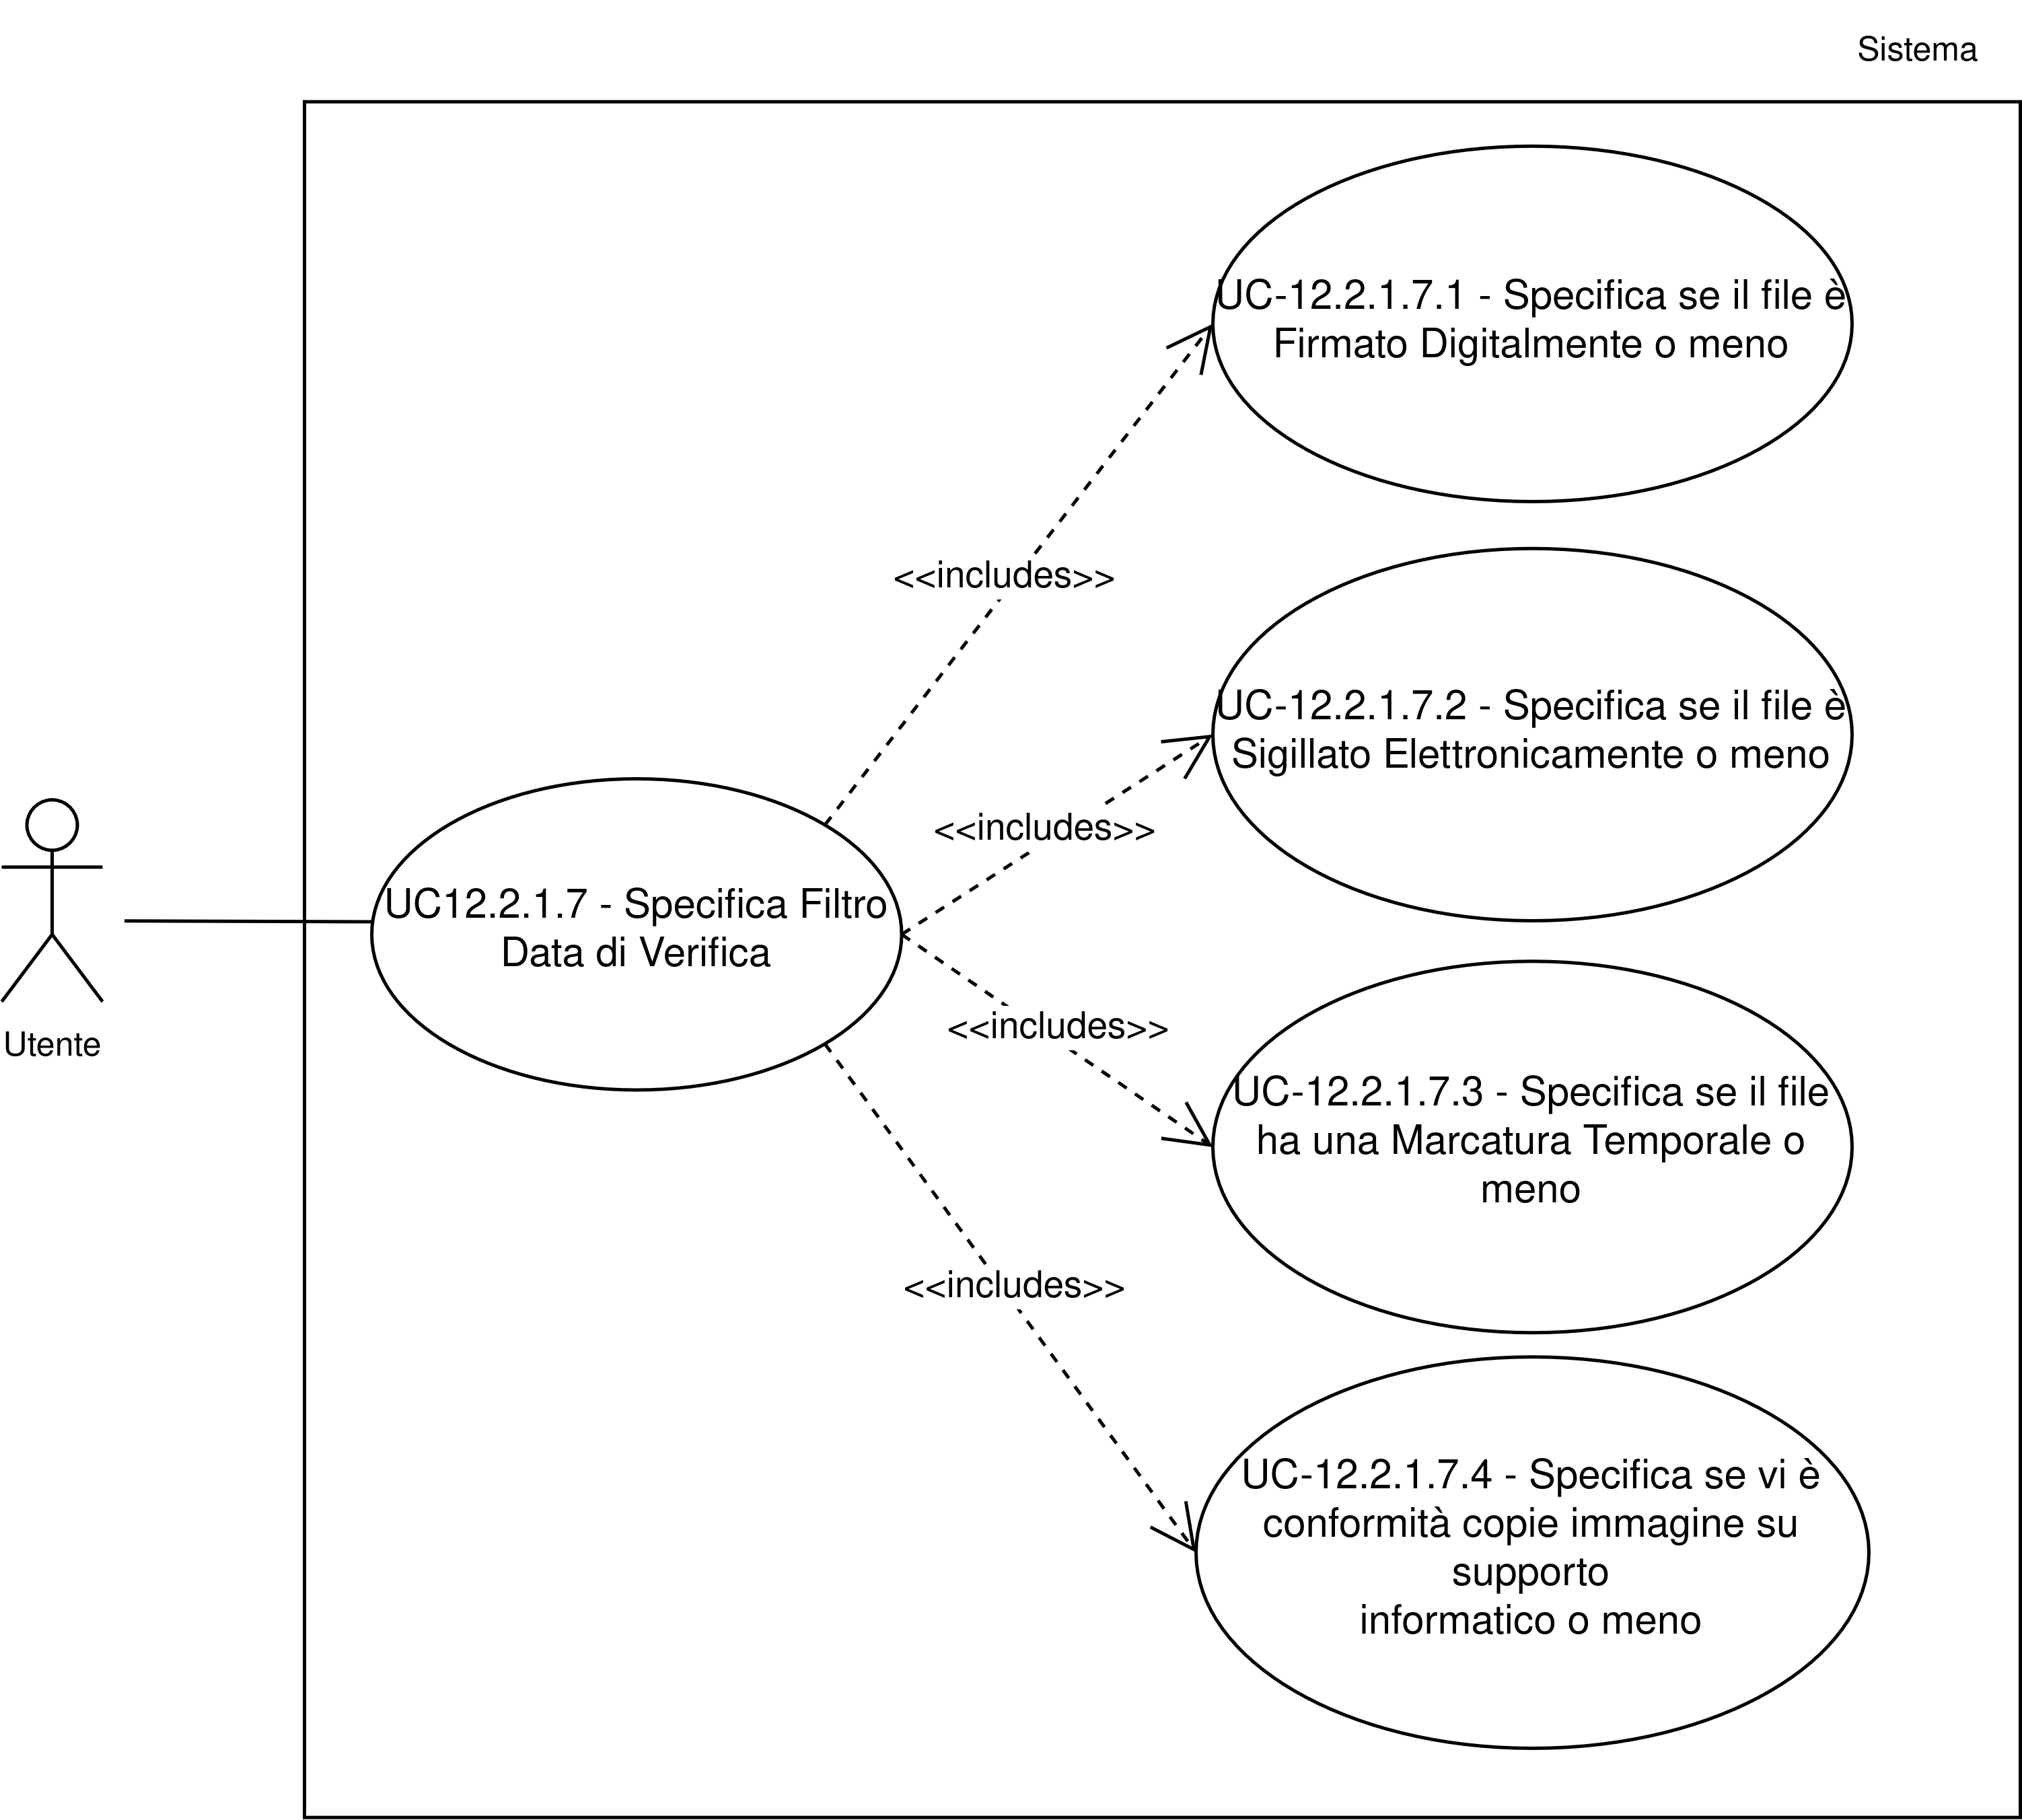
\includegraphics[width=1\textwidth]{../../assets/uml/UC12.2.1.7.png}
      \caption{Inclusioni \ref{addDatiVerifica} - Specifica filtro Dati di Verifica}
      \label{fig:inclusioniSpecificaFiltriDatiVerifica}
\end{figure}
\begin{itemize}
      \item \textbf{Attore Primario}: Utente
      \item \textbf{Precondizioni}: 
      \begin{itemize}
            \item L'Utente ha avviato l'applicazione
            \item L'Utente sta effettuando una ricerca nel DIP con filtri
            \item L'Utente ha specificato come tipo di documento: Documento Informatico o Documento Amministrativo Informatico
            \item L'utente ha selezionato il filtro Dati di Verifica tra i campi specifici per tipo documentale
      \end{itemize}
      \item \textbf{Postcondizioni}: \begin{itemize}
            \item L'Utente ha specificato i valori del filtro Dati di Verifica
            \item Il filtro Dati di Verifica è parametro per la ricerca con filtri e per la generazione del risultato
      \end{itemize}
      \item \textbf{Flusso Principale}:
      \begin{enumerate}
            \item L'Utente specifica se il file è Firmato Digitalmente o meno (\ref{addValoreFirmaDigitalePresente})
            \item L'Utente specifica se il file è Sigillato Elettronicamente o meno (\ref{addValoreSigilloElettronicoPresente})
            \item L'Utente specifica se il file ha una Marcatura Temporale o meno (\ref{addValoreMarcaturaTemporalePresente})
            \item L'Utente specifica se vi è conformità copie immagine su supporto informatico o meno (\ref{addValoreConformitaCopieImmagine})
            \item Il sistema imposta i valori del filtro come parametri di ricerca
      \end{enumerate}
      \item \textbf{Inclusioni}: 
      \begin{itemize} 
            \item \ref{addValoreFirmaDigitalePresente} - Specifica se il file è Firmato Digitalmente o meno
            \item \ref{addValoreSigilloElettronicoPresente} - Specifica se il file è Sigillato Elettronicamente o meno
            \item \ref{addValoreMarcaturaTemporalePresente} - Specifica se il file ha una Marcatura Temporale o meno
            \item \ref{addValoreConformitaCopieImmagine} - Specifica se vi è conformità copie immagine su supporto informatico o meno
      \end{itemize}
\end{itemize}

\subdeepusecase{addValoreFirmaDigitalePresente}{Specifica se il file è Firmato Digitalmente o meno}\label{addValoreFirmaDigitalePresente}
\begin{itemize}
      \item \textbf{Attore Primario}: Utente
      \item \textbf{Precondizioni}: 
      \begin{itemize}
            \item L'Utente ha avviato l'applicazione
            \item L'Utente sta effettuando una ricerca nel DIP con filtri
            \item L'Utente ha specificato come tipo di documento: Documento Informatico o Documento Amministrativo Informatico
            \item L'utente ha selezionato il filtro Dati di Verifica tra i campi specifici per tipo documentale
      \end{itemize}
      \item \textbf{Postcondizioni}: Il sistema riceve se il file è Firmato Digitalmente o meno e lo salva per il filtro Dati di Verifica.
      \item \textbf{Flusso Principale}:
      \begin{enumerate}
            \item L'Utente specifica se il file è Firmato Digitalmente o meno (sì/no).
            \item Il sistema riceve se il file è Firmato Digitalmente o meno e lo salva per il filtro Dati di Verifica.
      \end{enumerate}
\end{itemize}

\subdeepusecase{addValoreSigilloElettronicoPresente}{Specifica se il file è Sigillato Elettronicamente o meno}\label{addValoreSigilloElettronicoPresente}
\begin{itemize}
      \item \textbf{Attore Primario}: Utente
      \item \textbf{Precondizioni}: 
      \begin{itemize}
            \item L'Utente ha avviato l'applicazione
            \item L'Utente sta effettuando una ricerca nel DIP con filtri
            \item L'Utente ha specificato come tipo di documento: Documento Informatico o Documento Amministrativo Informatico
            \item L'utente ha selezionato il filtro Dati di Verifica tra i campi specifici per tipo documentale
      \end{itemize}
      \item \textbf{Postcondizioni}: Il sistema riceve se il file è Sigillato Elettronicamente o meno e lo salva per il filtro Dati di Verifica.
      \item \textbf{Flusso Principale}:
      \begin{enumerate}
            \item L'Utente specifica se il file è Sigillato Elettronicamente o meno (sì/no).
            \item Il sistema riceve se il file è Sigillato Elettronicamente o meno e lo salva per il filtro Dati di Verifica.
      \end{enumerate}
\end{itemize}

\subdeepusecase{addValoreMarcaturaTemporalePresente}{Specifica se il file ha una Marcatura Temporale o meno}\label{addValoreMarcaturaTemporalePresente}
\begin{itemize}
      \item \textbf{Attore Primario}: Utente
      \item \textbf{Precondizioni}: 
      \begin{itemize}
            \item L'Utente ha avviato l'applicazione
            \item L'Utente sta effettuando una ricerca nel DIP con filtri
            \item L'Utente ha specificato come tipo di documento: Documento Informatico o Documento Amministrativo Informatico
            \item L'utente ha selezionato il filtro Dati di Verifica tra i campi specifici per tipo documentale
      \end{itemize}
      \item \textbf{Postcondizioni}: Il sistema riceve se il file ha una Marcatura Temporale o meno e lo salva per il filtro Dati di Verifica.
      \item \textbf{Flusso Principale}:
      \begin{enumerate}
            \item L'Utente specifica se il file ha una Marcatura Temporale o meno (sì/no).
            \item Il sistema riceve se il file ha una Marcatura Temporale o meno e lo salva per il filtro Dati di Verifica.
      \end{enumerate}
\end{itemize}

\subdeepusecase{addValoreConformitaCopieImmagine}{Specifica se vi è conformità copie immagine su supporto informatico o meno}\label{addValoreConformitaCopieImmagine}
\begin{itemize}
      \item \textbf{Attore Primario}: Utente
      \item \textbf{Precondizioni}: 
      \begin{itemize}
            \item L'Utente ha avviato l'applicazione
            \item L'Utente sta effettuando una ricerca nel DIP con filtri
            \item L'Utente ha specificato come tipo di documento: Documento Informatico o Documento Amministrativo Informatico
            \item L'utente ha selezionato il filtro Dati di Verifica tra i campi specifici per tipo documentale
      \end{itemize}
      \item \textbf{Postcondizioni}: Il sistema riceve se vi è conformità copie immagine su supporto informatico o meno e lo salva per il filtro Dati di Verifica.
      \item \textbf{Flusso Principale}:
      \begin{enumerate}
            \item L'Utente specifica se vi è conformità copie immagine su supporto informatico o meno (sì/no).
            \item Il sistema riceve se vi è conformità copie immagine su supporto informatico o meno e lo salva per il filtro Dati di Verifica.
      \end{enumerate}
\end{itemize}

\deepusecase{addNomeDocumento}{Specifica filtro Nome del Documento}
\begin{figure}[H]
      \centering
      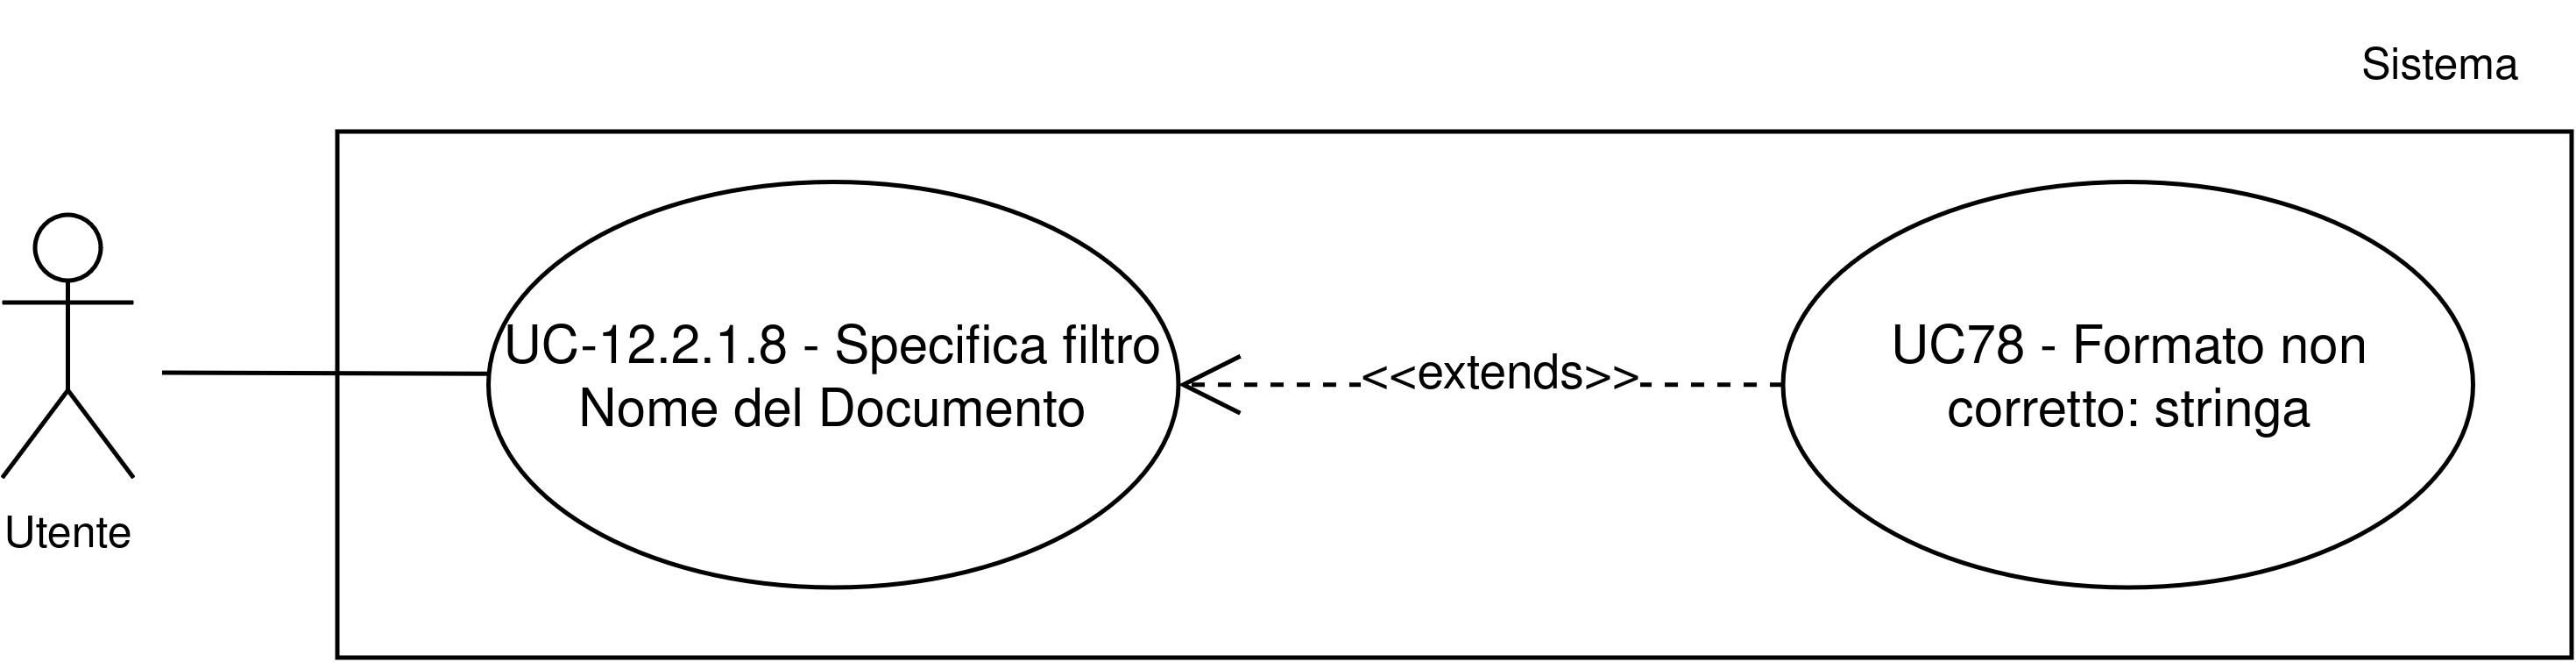
\includegraphics[width=1\textwidth]{../../assets/uml/UC12.2.1.8.png}
      \caption{Inclusioni \ref{addDatiVerifica} - Specifica filtro Dati di Verifica}
      \label{fig:inclusioniSpecificaFiltriDatiVerifica}
\end{figure}
\begin{itemize}
      \item \textbf{Attore Primario}: Utente
      \item \textbf{Precondizioni}: 
      \begin{itemize}
            \item L'Utente ha avviato l'applicazione
            \item L'Utente sta effettuando una ricerca nel DIP con filtri
            \item L'Utente ha specificato come tipo di documento: Documento Informatico o Documento Amministrativo Informatico
            \item L'utente ha selezionato il filtro Nome del Documento tra i campi specifici per tipo documentale
      \end{itemize}
      \item \textbf{Postcondizioni}: \begin{itemize}
            \item L'Utente ha specificato i valori del filtro Nome del Documento
            \item Il filtro Nome del Documento è parametro per la ricerca con filtri e per la generazione del risultato
      \end{itemize}
      \item \textbf{Flusso Principale}:
            \begin{enumerate}
                  \item L'Utente specifica il Nome del Documento
                  \item Il sistema imposta questo valore come parametro per la ricerca
            \end{enumerate}
      \item \textbf{Flusso Alternativo}:
      \begin{itemize}
            \item L'Utente inserisce un nome non valido per il filtro Nome del Documento (stringa vuota) (\ref{formatoNonCorrettoStringa})
      \end{itemize}
      \item \textbf{Estensioni}: \ref{formatoNonCorrettoStringa} Formato non corretto: stringa
\end{itemize}

\deepusecase{addVersioneDocumento}{Specifica filtro Versione del Documento}
\begin{figure}[H]
      \centering
      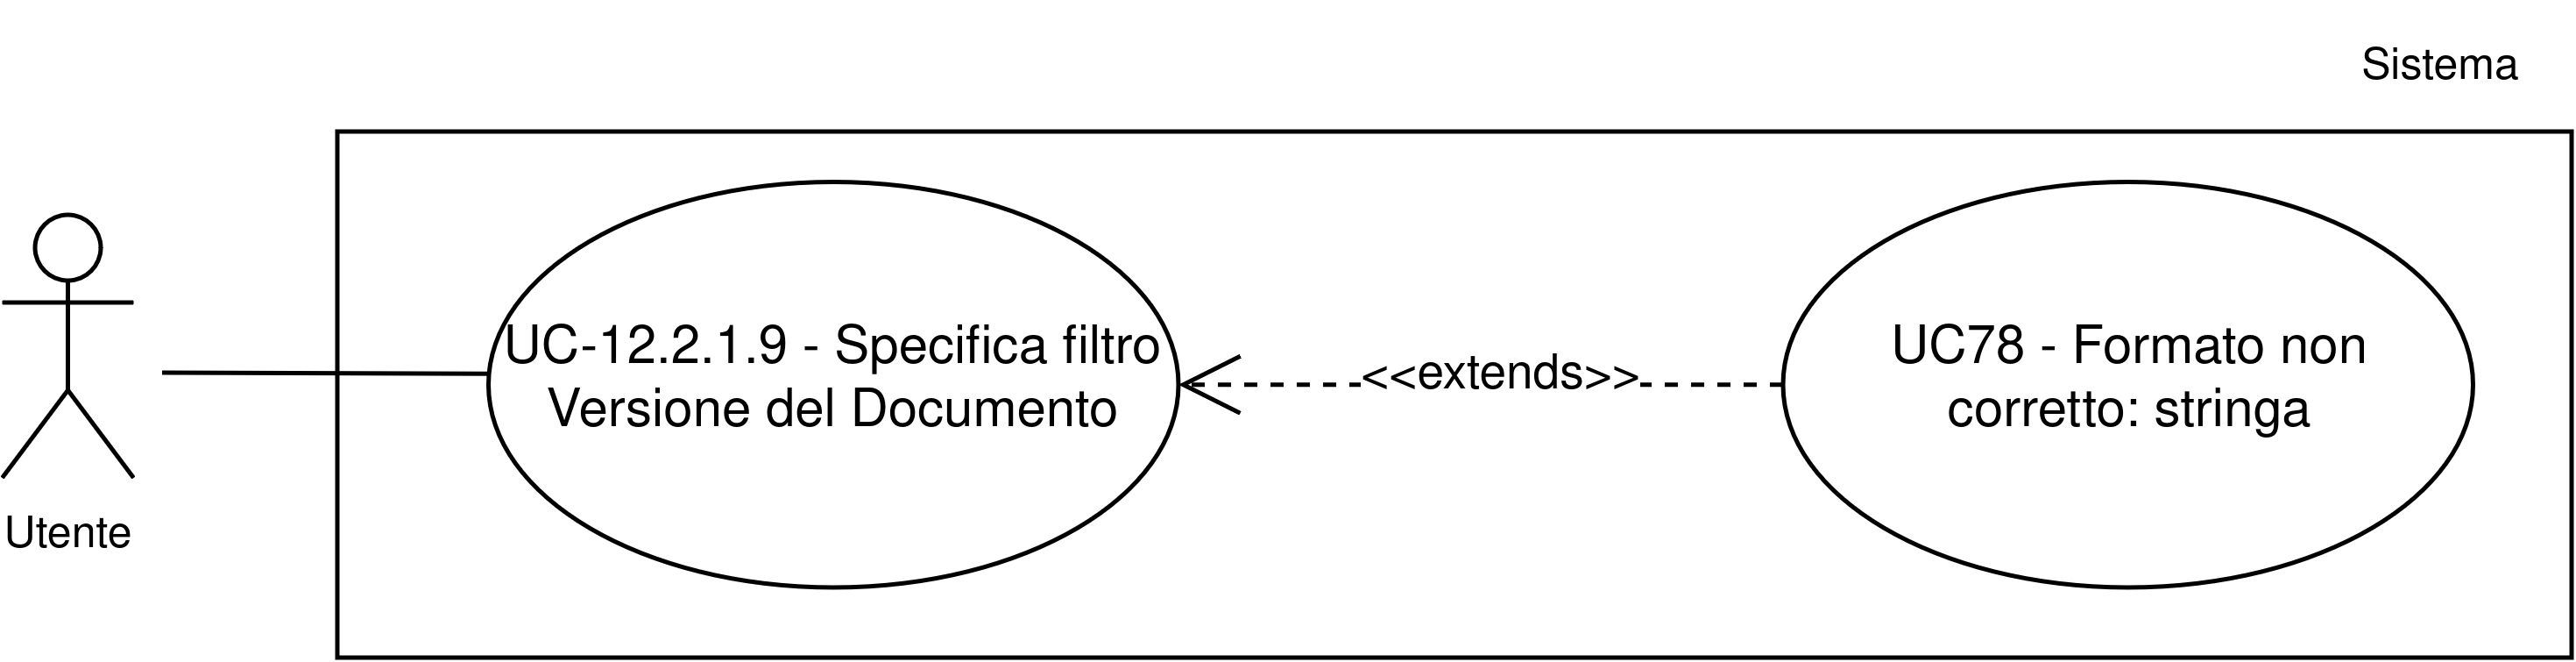
\includegraphics[width=1\textwidth]{../../assets/uml/UC12.2.1.9.png}
      \caption{Inclusioni \ref{addVersioneDocumento} - Specifica filtro Versione del Documento}
      \label{fig:inclusioniSpecificaFiltriVersioneDocumento}
\end{figure}
\begin{itemize}
      \item \textbf{Attore Primario}: Utente
      \item \textbf{Precondizioni}: 
      \begin{itemize}
            \item L'Utente ha avviato l'applicazione
            \item L'Utente sta effettuando una ricerca nel DIP con filtri
            \item L'Utente ha specificato come tipo di documento: Documento Informatico o Documento Amministrativo Informatico
            \item L'utente ha selezionato il filtro Versione del Documento tra i campi specifici per tipo documentale
      \end{itemize}
      \item \textbf{Postcondizioni}: \begin{itemize}
            \item L'Utente ha specificato i valori del filtro Versione del Documento
            \item Il filtro Versione del Documento è parametro per la ricerca con filtri e per la generazione del risultato
      \end{itemize}
      \item \textbf{Flusso Principale}:
            \begin{enumerate}
                  \item L'Utente specifica il numero che rappresenta la Versione del Documento.
                  \item Il sistema imposta questo valore come parametro per la ricerca.
            \end{enumerate}
      \item \textbf{Flusso Alternativo}:
      \begin{itemize}
            \item L'Utente inserisce una versione non valida per il filtro Versione del Documento (stringa vuota) (\ref{formatoNonCorrettoStringa})
      \end{itemize}
      \item \textbf{Estensioni}: \ref{formatoNonCorrettoStringa} Formato non corretto: stringa
\end{itemize}

\deepusecase{addIdentificativoDocumentoPrimario}{Specifica filtro Identificativo del Documento Primario}
\begin{figure}[H]
      \centering
      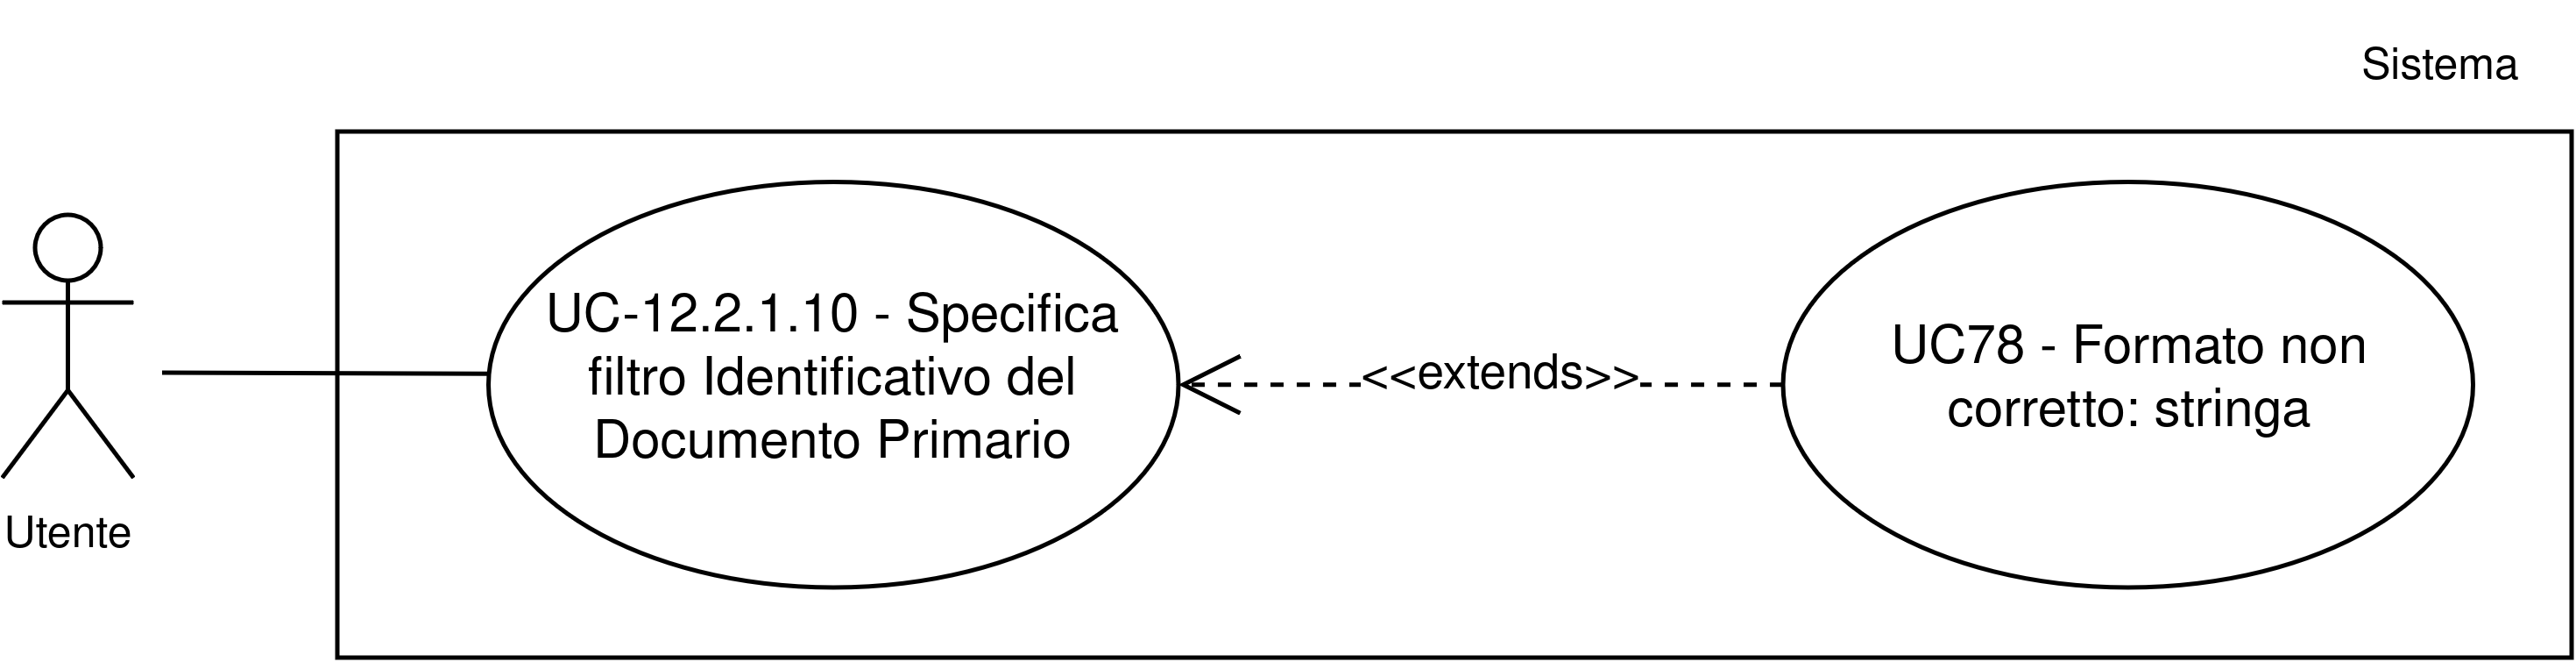
\includegraphics[width=1\textwidth]{../../assets/uml/UC12.2.1.10.png}
      \caption{Inclusioni \ref{addIdentificativoDocumentoPrimario} - Specifica filtro Identificativo del Documento Primario}
      \label{fig:inclusioniSpecificaFiltriIdentificativoDocumentoPrimario}
\end{figure}
\begin{itemize}
      \item \textbf{Attore Primario}: Utente
      \item \textbf{Precondizioni}:
      \begin{itemize}
            \item L'Utente ha avviato l'applicazione
            \item L'Utente sta effettuando una ricerca nel DIP con filtri
            \item L'Utente ha specificato come tipo di documento: Documento Informatico o Documento Amministrativo Informatico
            \item L'utente ha selezionato il filtro Identificativo del Documento Primario tra i campi specifici per tipo documentale
      \end{itemize}
      \item \textbf{Postcondizioni}: \begin{itemize}
            \item L'Utente ha specificato i valori del filtro Identificativo del Documento Primario
            \item Il filtro Identificativo del Documento Primario è parametro per la ricerca con filtri e per la generazione del risultato
      \end{itemize}
      \item \textbf{Flusso Principale}:
            \begin{enumerate}
                  \item L'Utente specifica l'Identificativo del Documento Primario.
                  \item Il sistema imposta questo valore come parametro per la ricerca.
            \end{enumerate}
      \item \textbf{Flusso Alternativo}:
      \begin{itemize}
            \item L'Utente inserisce un identificativo non valido per il filtro Identificativo del Documento Primario (stringa vuota) (\ref{formatoNonCorrettoStringa})
      \end{itemize}
      \item \textbf{Estensioni}: \ref{formatoNonCorrettoStringa} Formato non corretto: stringa
\end{itemize}

\deepusecase{addTracciatureModificheDocumento}{Specifica filtro Tracciature Modifiche di Documento}
\begin{figure}[H]
      \centering
      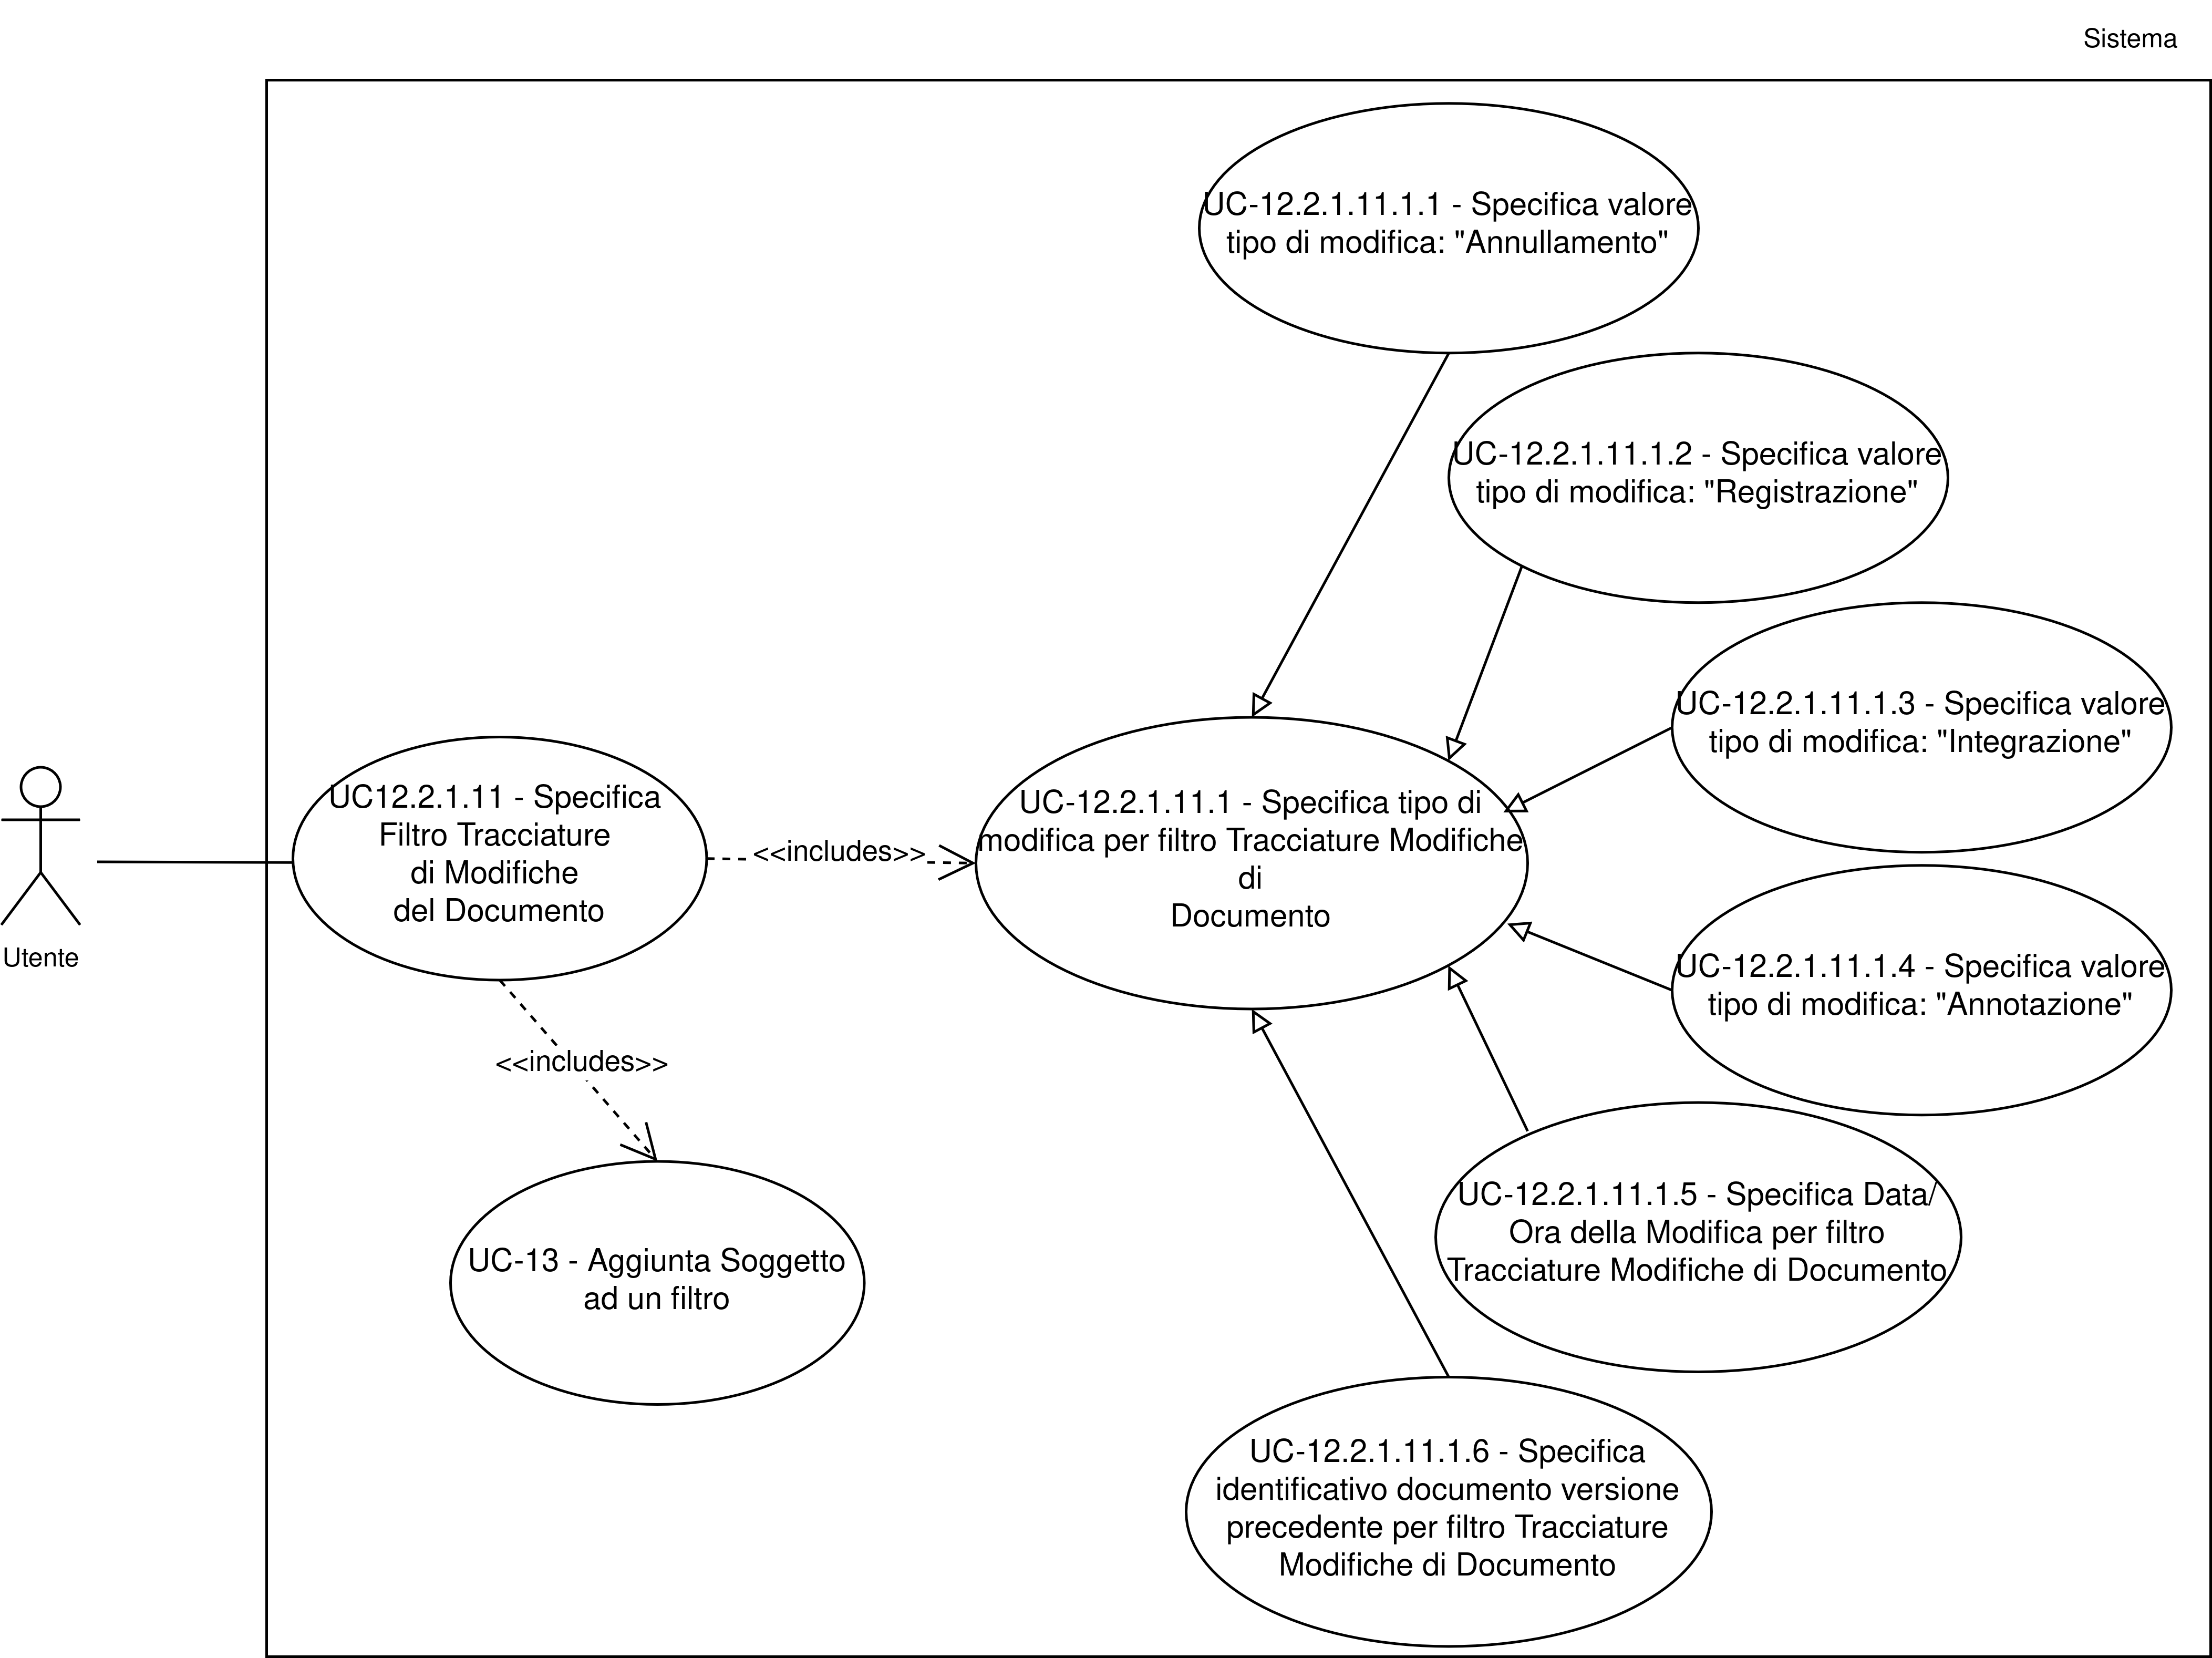
\includegraphics[width=1\textwidth]{../../assets/uml/UC12.2.1.11.png}
      \caption{Inclusioni \ref{addTracciatureModificheDocumento} - Specifica filtro Tracciature Modifiche di Documento}
      \label{fig:inclusioniSpecificaFiltriTracciatureModificheDocumento}
\end{figure}
\begin{itemize}
      \item \textbf{Attore Primario}: Utente
      \item \textbf{Precondizioni}: 
      \begin{itemize}
            \item L'Utente ha avviato l'applicazione
            \item L'Utente sta effettuando una ricerca nel DIP con filtri
            \item L'Utente ha specificato come tipo di documento: Documento Informatico o Documento Amministrativo Informatico
            \item L'utente ha selezionato il filtro Tracciature Modifiche di Documento tra i campi specifici per tipo documentale
      \end{itemize}
      \item \textbf{Postcondizioni}: \begin{itemize}
            \item L'Utente ha specificato i valori del filtro Tracciature Modifiche di Documento
            \item Il filtro Tracciature Modifiche di Documento è parametro per la ricerca con filtri e per la generazione del risultato
      \end{itemize}
      \item \textbf{Flusso Principale}:
            \begin{enumerate}
                  \item L'Utente sceglie il Tipo di modifica. (\ref{addValoreTipoModifica})
                  \item L'Utente specifica il Soggetto che ha effettuato la modifica. (\ref{addSoggetto})
                  \item L'Utente specifica la Data/Ora della Modifica.
                  \item L'Utente specifica l'identificativo documento versione precedente.
                  \item Il sistema imposta i valori del filtro come parametri di ricerca.
            \end{enumerate}
      \item \textbf{Inclusioni}: 
      \begin{itemize}
            \item \ref{addValoreTipoModifica} - Specifica tipo di modifica per filtro Tracciature Modifiche di Documento
            \item \ref{addSoggetto} - Specifica soggetto che ha effettuato la modifica per filtro Tracciature Modifiche di Documento
      \end{itemize}
\end{itemize}

\subdeepusecase{addValoreTipoModifica}{Specifica tipo di modifica per filtro Tracciature Modifiche di Documento}
\begin{itemize}
      \item \textbf{Attore Primario}: Utente
      \item \textbf{Precondizioni}: 
      \begin{itemize}            
            \item L'Utente ha avviato l'applicazione
            \item L'Utente sta effettuando una ricerca nel DIP con filtri
            \item L'Utente ha specificato come tipo di documento: Documento Informatico o Documento Amministrativo Informatico
            \item L'utente ha selezionato il filtro Tracciature Modifiche di Documento tra i campi specifici per tipo documentale
      \end{itemize}
      \item \textbf{Postcondizioni}: Vengono specificati i valori del Tipo di Modifica e salvati per il filtro Tracciature Modifiche di Documento.
      \item \textbf{Flusso Principale}:
            \begin{enumerate}
                  \item L'Utente specifica il tipo di modifica.
                  \item Il sistema salva il valore del tipo di modifica per il filtro Tracciature Modifiche di Documento.
            \end{enumerate}
\end{itemize}

\subsubdeepusecase{addValoreTipoModificaAnnullamento}{Specifica valore tipo di modifica: "Annullamento"}
\begin{itemize}
      \item \textbf{Attore Primario}: Utente
      \item \textbf{Precondizioni}: 
      \begin{itemize}            
            \item L'Utente ha avviato l'applicazione
            \item L'Utente sta effettuando una ricerca nel DIP con filtri
            \item L'Utente ha specificato come tipo di documento: Documento Informatico o Documento Amministrativo Informatico
            \item L'utente ha selezionato il filtro Tracciature Modifiche di Documento tra i campi specifici per tipo documentale
      \end{itemize}
      \item \textbf{Postcondizioni}: Viene selezionato "Annullamento" come valore del tipo di modifica e salvato per il filtro Tracciature Modifiche di Documento.
      \item \textbf{Flusso Principale}:
            \begin{enumerate}
                  \item L'Utente specifica il valore del tipo di modifica: "Annullamento".
                  \item Il sistema salva il valore del tipo di modifica per il filtro Tracciature Modifiche di Documento.
            \end{enumerate}
      \item \textbf{Specializza}: \ref{addValoreTipoModifica}
\end{itemize}

\subsubdeepusecase{addValoreTipoModificaRegistrazione}{Specifica valore tipo di modifica: "Registrazione"}
\begin{itemize}
      \item \textbf{Attore Primario}: Utente
      \item \textbf{Precondizioni}: 
      \begin{itemize}            
            \item L'Utente ha avviato l'applicazione
            \item L'Utente sta effettuando una ricerca nel DIP con filtri
            \item L'Utente ha specificato come tipo di documento: Documento Informatico o Documento Amministrativo Informatico
            \item L'utente ha selezionato il filtro Tracciature Modifiche di Documento tra i campi specifici per tipo documentale
      \end{itemize}
      \item \textbf{Postcondizioni}: Viene selezionato "Registrazione" come valore del tipo di modifica e salvato per il filtro Tracciature Modifiche di Documento.
      \item \textbf{Flusso Principale}:
            \begin{enumerate}
                  \item L'Utente specifica il valore del tipo di modifica: "Registrazione".
                  \item Il sistema salva il valore del tipo di modifica per il filtro Tracciature Modifiche di Documento.
            \end{enumerate}
      \item \textbf{Specializza}: \ref{addValoreTipoModifica}
\end{itemize}

\subsubdeepusecase{addValoreTipoModificaIntegrazione}{Specifica valore tipo di modifica: "Integrazione"}
\begin{itemize}
      \item \textbf{Attore Primario}: Utente
      \item \textbf{Precondizioni}: 
      \begin{itemize}            
            \item L'Utente ha avviato l'applicazione
            \item L'Utente sta effettuando una ricerca nel DIP con filtri
            \item L'Utente ha specificato come tipo di documento: Documento Informatico o Documento Amministrativo Informatico
            \item L'utente ha selezionato il filtro Tracciature Modifiche di Documento tra i campi specifici per tipo documentale
      \end{itemize}
      \item \textbf{Postcondizioni}: Viene selezionato "Integrazione" come valore del tipo di modifica e salvato per il filtro Tracciature Modifiche di Documento.
      \item \textbf{Flusso Principale}:
            \begin{enumerate}
                  \item L'Utente specifica il valore del tipo di modifica: "Integrazione".
                  \item Il sistema salva il valore del tipo di modifica per il filtro Tracciature Modifiche di Documento.
            \end{enumerate}
      \item \textbf{Specializza}: \ref{addValoreTipoModifica}
\end{itemize}

\subsubdeepusecase{addValoreTipoModificaAnnotazione}{Specifica valore tipo di modifica: "Annotazione"}
\begin{itemize}
      \item \textbf{Attore Primario}: Utente
      \item \textbf{Precondizioni}: 
      \begin{itemize}            
            \item L'Utente ha avviato l'applicazione
            \item L'Utente sta effettuando una ricerca nel DIP con filtri
            \item L'Utente ha specificato come tipo di documento: Documento Informatico o Documento Amministrativo Informatico
            \item L'utente ha selezionato il filtro Tracciature Modifiche di Documento tra i campi specifici per tipo documentale
      \end{itemize}
      \item \textbf{Postcondizioni}: Viene selezionato "Annotazione" come valore del tipo di modifica e salvato per il filtro Tracciature Modifiche di Documento.
      \item \textbf{Flusso Principale}:
            \begin{enumerate}
                  \item L'Utente specifica il valore del tipo di modifica: "Annotazione".
                  \item Il sistema salva il valore del tipo di modifica per il filtro Tracciature Modifiche di Documento.
            \end{enumerate}
      \item \textbf{Specializza}: \ref{addValoreTipoModifica}
\end{itemize}

\subsubdeepusecase{addValoreDataOraModifica}{Specifica Data/Ora della Modifica per filtro Tracciature Modifiche di Documento}
\begin{itemize}
      \item \textbf{Attore Primario}: Utente
      \item \textbf{Precondizioni}: 
      \begin{itemize}            
            \item L'Utente ha avviato l'applicazione
            \item L'Utente sta effettuando una ricerca nel DIP con filtri
            \item L'Utente ha specificato come tipo di documento: Documento Informatico o Documento Amministrativo Informatico
            \item L'utente ha selezionato il filtro Tracciature Modifiche di Documento tra i campi specifici per tipo documentale
      \end{itemize}
      \item \textbf{Postcondizioni}: Viene specificata la Data/Ora della Modifica e salvata per il filtro Tracciature Modifiche di Documento.
      \item \textbf{Flusso Principale}:
            \begin{enumerate}
                  \item L'Utente specifica la Data/Ora della Modifica.
                  \item Il sistema salva il valore del filtro Data/Ora della Modifica.
            \end{enumerate}
      \item \textbf{Flusso Alternativo}:
      \begin{itemize}
            \item L'Utente inserisce una data non valida per il filtro Data/Ora della Modifica (formato data errato) (\ref{formatoNonCorrettoData})
      \end{itemize}
      \item \textbf{Estensioni}: \ref{formatoNonCorrettoData} Formato non corretto: data
\end{itemize}

\subsubdeepusecase{addValoreIdVersionePrecedente}{Specifica identificativo documento versione precedente per filtro Tracciature Modifiche di Documento}
\begin{itemize}
      \item \textbf{Attore Primario}: Utente
      \item \textbf{Precondizioni}: 
      \begin{itemize}            
            \item L'Utente ha avviato l'applicazione
            \item L'Utente sta effettuando una ricerca nel DIP con filtri
            \item L'Utente ha specificato come tipo di documento: Documento Informatico o Documento Amministrativo Informatico
            \item L'utente ha selezionato il filtro Tracciature Modifiche di Documento tra i campi specifici per tipo documentale
      \end{itemize}
      \item \textbf{Postcondizioni}: Viene specificato l'identificativo documento versione precedente e salvato per il filtro Tracciature Modifiche di Documento.
      \item \textbf{Flusso Principale}:
            \begin{enumerate}
                  \item L'Utente specifica l'identificativo documento versione precedente.
                  \item Il sistema salva il valore del filtro Identificativo documento versione precedente.
            \end{enumerate}
      \item \textbf{Flusso Alternativo}:
      \begin{itemize}
            \item L'Utente inserisce un identificativo non valido per il filtro Identificativo documento versione precedente (stringa vuota) (\ref{formatoNonCorrettoStringa})
      \end{itemize}
      \item \textbf{Estensioni}: \ref{formatoNonCorrettoStringa} Formato non corretto: stringa
\end{itemize}

\subsubusecase{specificaFiltriAggregazione}{Specifica filtri per Aggregazione Documentale Informatica}
\begin{figure}[H]
    \centering
    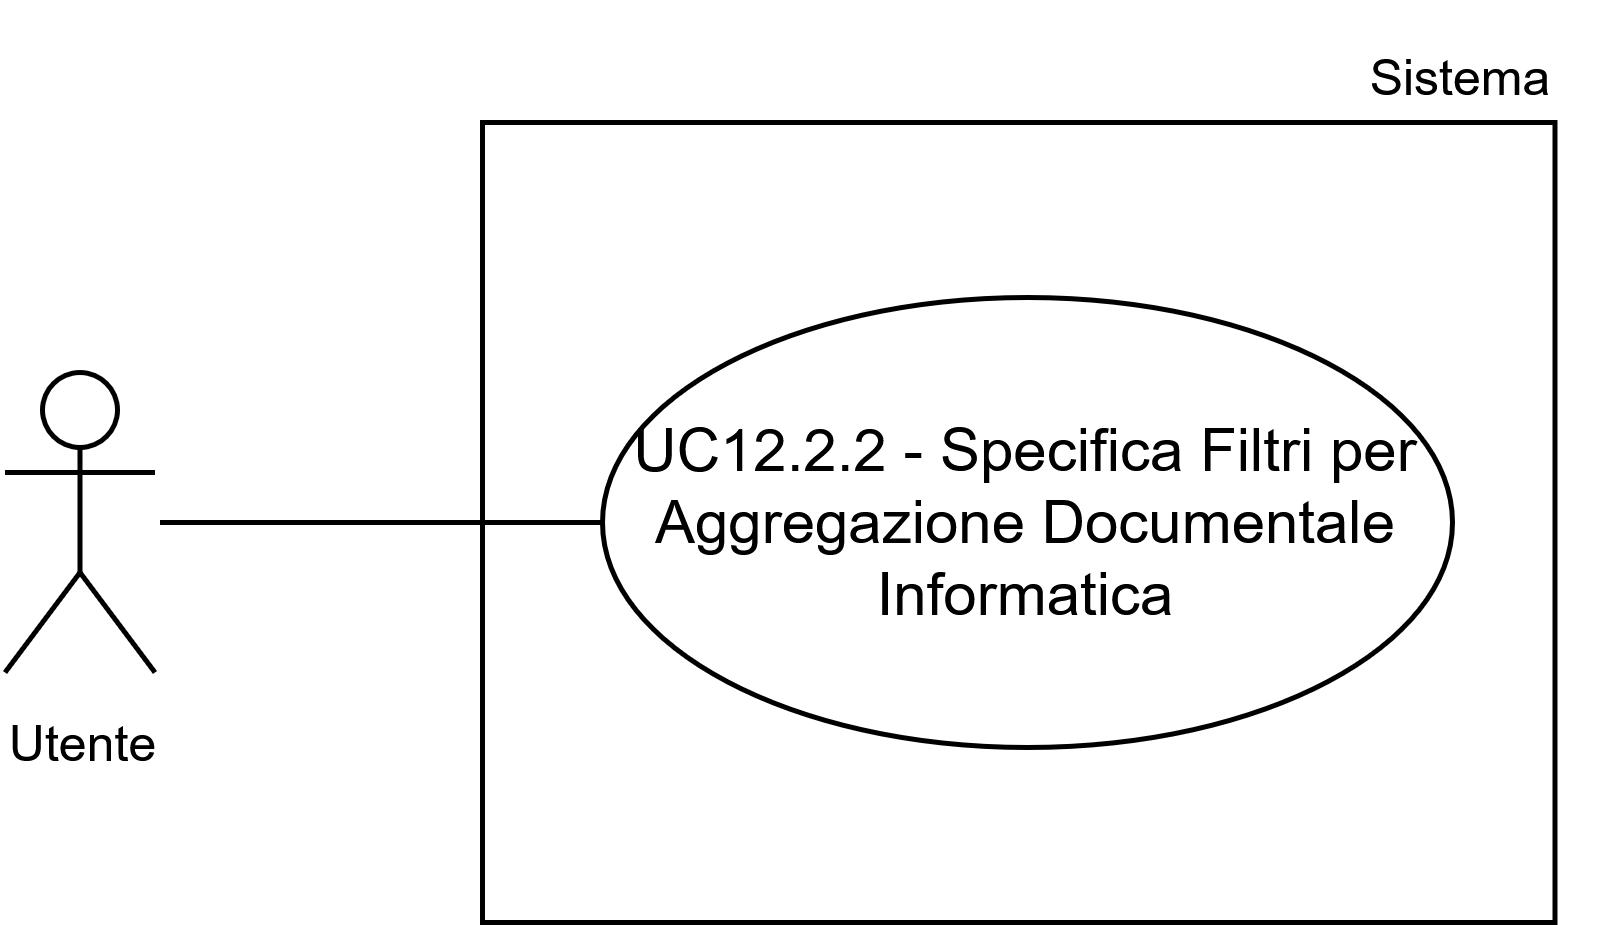
\includegraphics[width=0.6\textwidth]{../../assets/uml/UC12.2.2.png}
    \caption{\ref{specificaFiltriAggregazione} - Specifica filtri per Aggregazione Documentale}
    \label{fig:uc_specificaFiltriAggregazione}
\end{figure}
\begin{itemize}
      \item \textbf{Attore Primario}: Utente
      \item \textbf{Precondizioni}: 
      \begin{itemize}
            \item L'Utente ha avviato l'applicazione
            \item L'Utente sta effettuando una ricerca nel DIP con filtri
            \item L'Utente ha specificato come tipo di documento: Aggregazione Documentale
      \end{itemize}
      \item \textbf{Postcondizioni}: Vengono specificati i filtri per i campi dell'Aggregazione Documentale e utilizzati per la generazione del risultato.
      \item \textbf{Flusso Principale}:
      \begin{enumerate}
            \item L'Utente seleziona i campi specifici per l'Aggregazione Documentale su cui basare la ricerca (\ref{selezionaCampiAggregazioneDocumentale}).
            \item L'Utente aggiunge i filtri specifici per il tipo Aggregazione (descritto negli UC da \ref{addTipoAggregazione} a \ref{addProgressivoAggregazione}).
      \end{enumerate}
      \item \textbf{Inclusioni}:
      \begin{itemize}
            \item \ref{selezionaCampiAggregazioneDocumentale} Seleziona campi di ricerca per \glossario{Aggregazione Documentale}
            \item \ref{addTipoAggregazione} Specifica filtro Tipo di Aggregazione
            \item \ref{addIdAggregazione} Specifica filtro Id dell'Aggregazione
            \item \ref{addTipologiaFascicolo} Specifica filtro Tipologia di \glossario{Fascicolo}
            \item \ref{addIdAggregazionePrimario} Specifica filtro \glossario{Id Aggregazione Primario}
            \item \ref{addDataApertura} Specifica filtro Data di Apertura
            \item \ref{addDataChiusura} Specifica filtro Data di Chiusura
            \item \ref{addProcedimentoAmministrativo} Specifica filtro \glossario{Procedimento Amministrativo}
            \item \ref{addAssegnazione} Specifica filtro Assegnazione
            \item \ref{addProgressivoAggregazione} Specifica filtro Progressivo di Aggregazione
      \end{itemize}
      \item \textbf{Specializza}: \ref{addFiltriTipoDocumento} Specifiche filtri per Tipo di Documento
\end{itemize}
\begin{figure}[H]
      \centering
      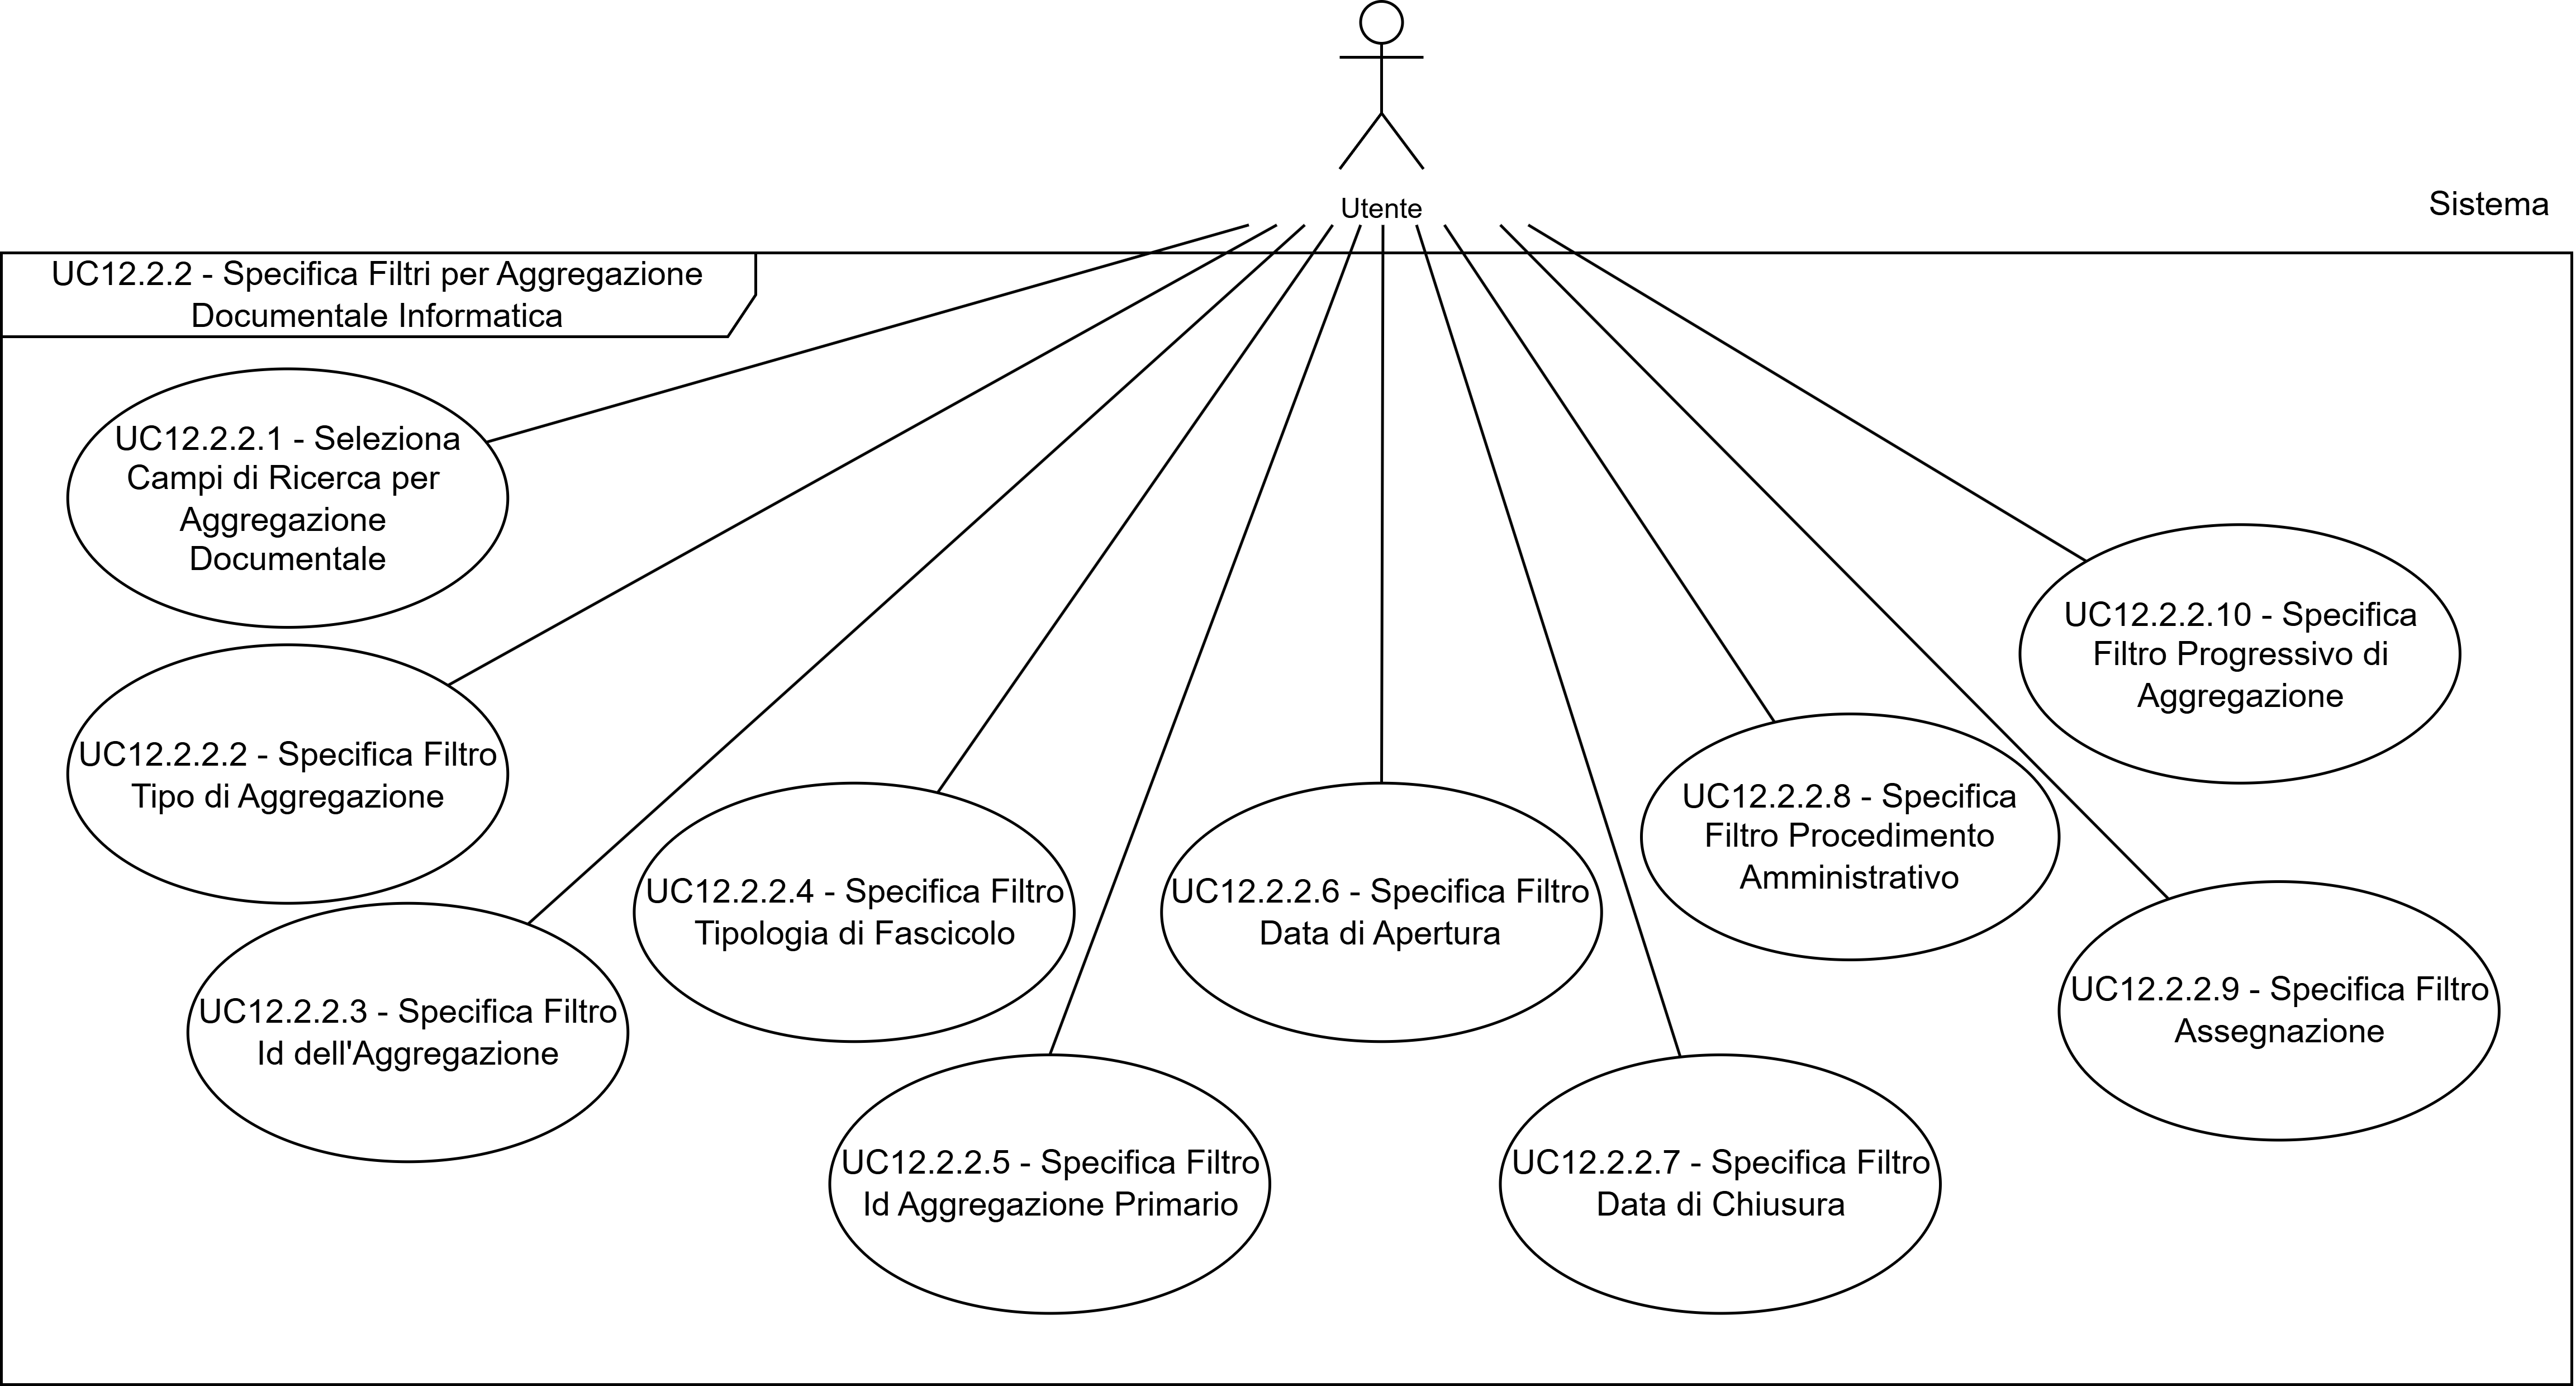
\includegraphics[width=1\textwidth]{../../assets/uml/UC12.2.2INC.png}
      \caption{Inclusioni \ref{specificaFiltriAggregazione} - Specifica filtri per Aggregazione Documentale}
      \label{fig:inclusioniSpecificaFiltriAggregazione}
\end{figure}

\deepusecase{selezionaCampiAggregazioneDocumentale}{Selezione campi di ricerca per Aggregazione Documentale}
\begin{itemize}
      \item \textbf{Attore Primario}: Utente
      \item \textbf{Precondizioni}: \begin{itemize}
            \item L'Utente ha avviato l'applicazione
            \item L'Utente sta effettuando una ricerca nel DIP con filtri
            \item L'Utente ha selezionato il filtro per il Tipo di Documento come Aggregazione Documentale
      \end{itemize}
      \item \textbf{Postcondizioni}:  I campi selezionati dall'Utente sono aggiunti ai campi selezionati per la ricerca.
      \item \textbf{Flusso Principale}:
      \begin{enumerate}
            \item L'Utente sceglie uno o più campi tra quelli disponibili.
            \item Il sistema aggiunge gli elementi selezionati ai campi selezionati per la ricerca.
      \end{enumerate}
\end{itemize}

\deepusecase{addTipoAggregazione}{Specifica filtro Tipo di Aggregazione}
\begin{figure}[H]
    \centering
    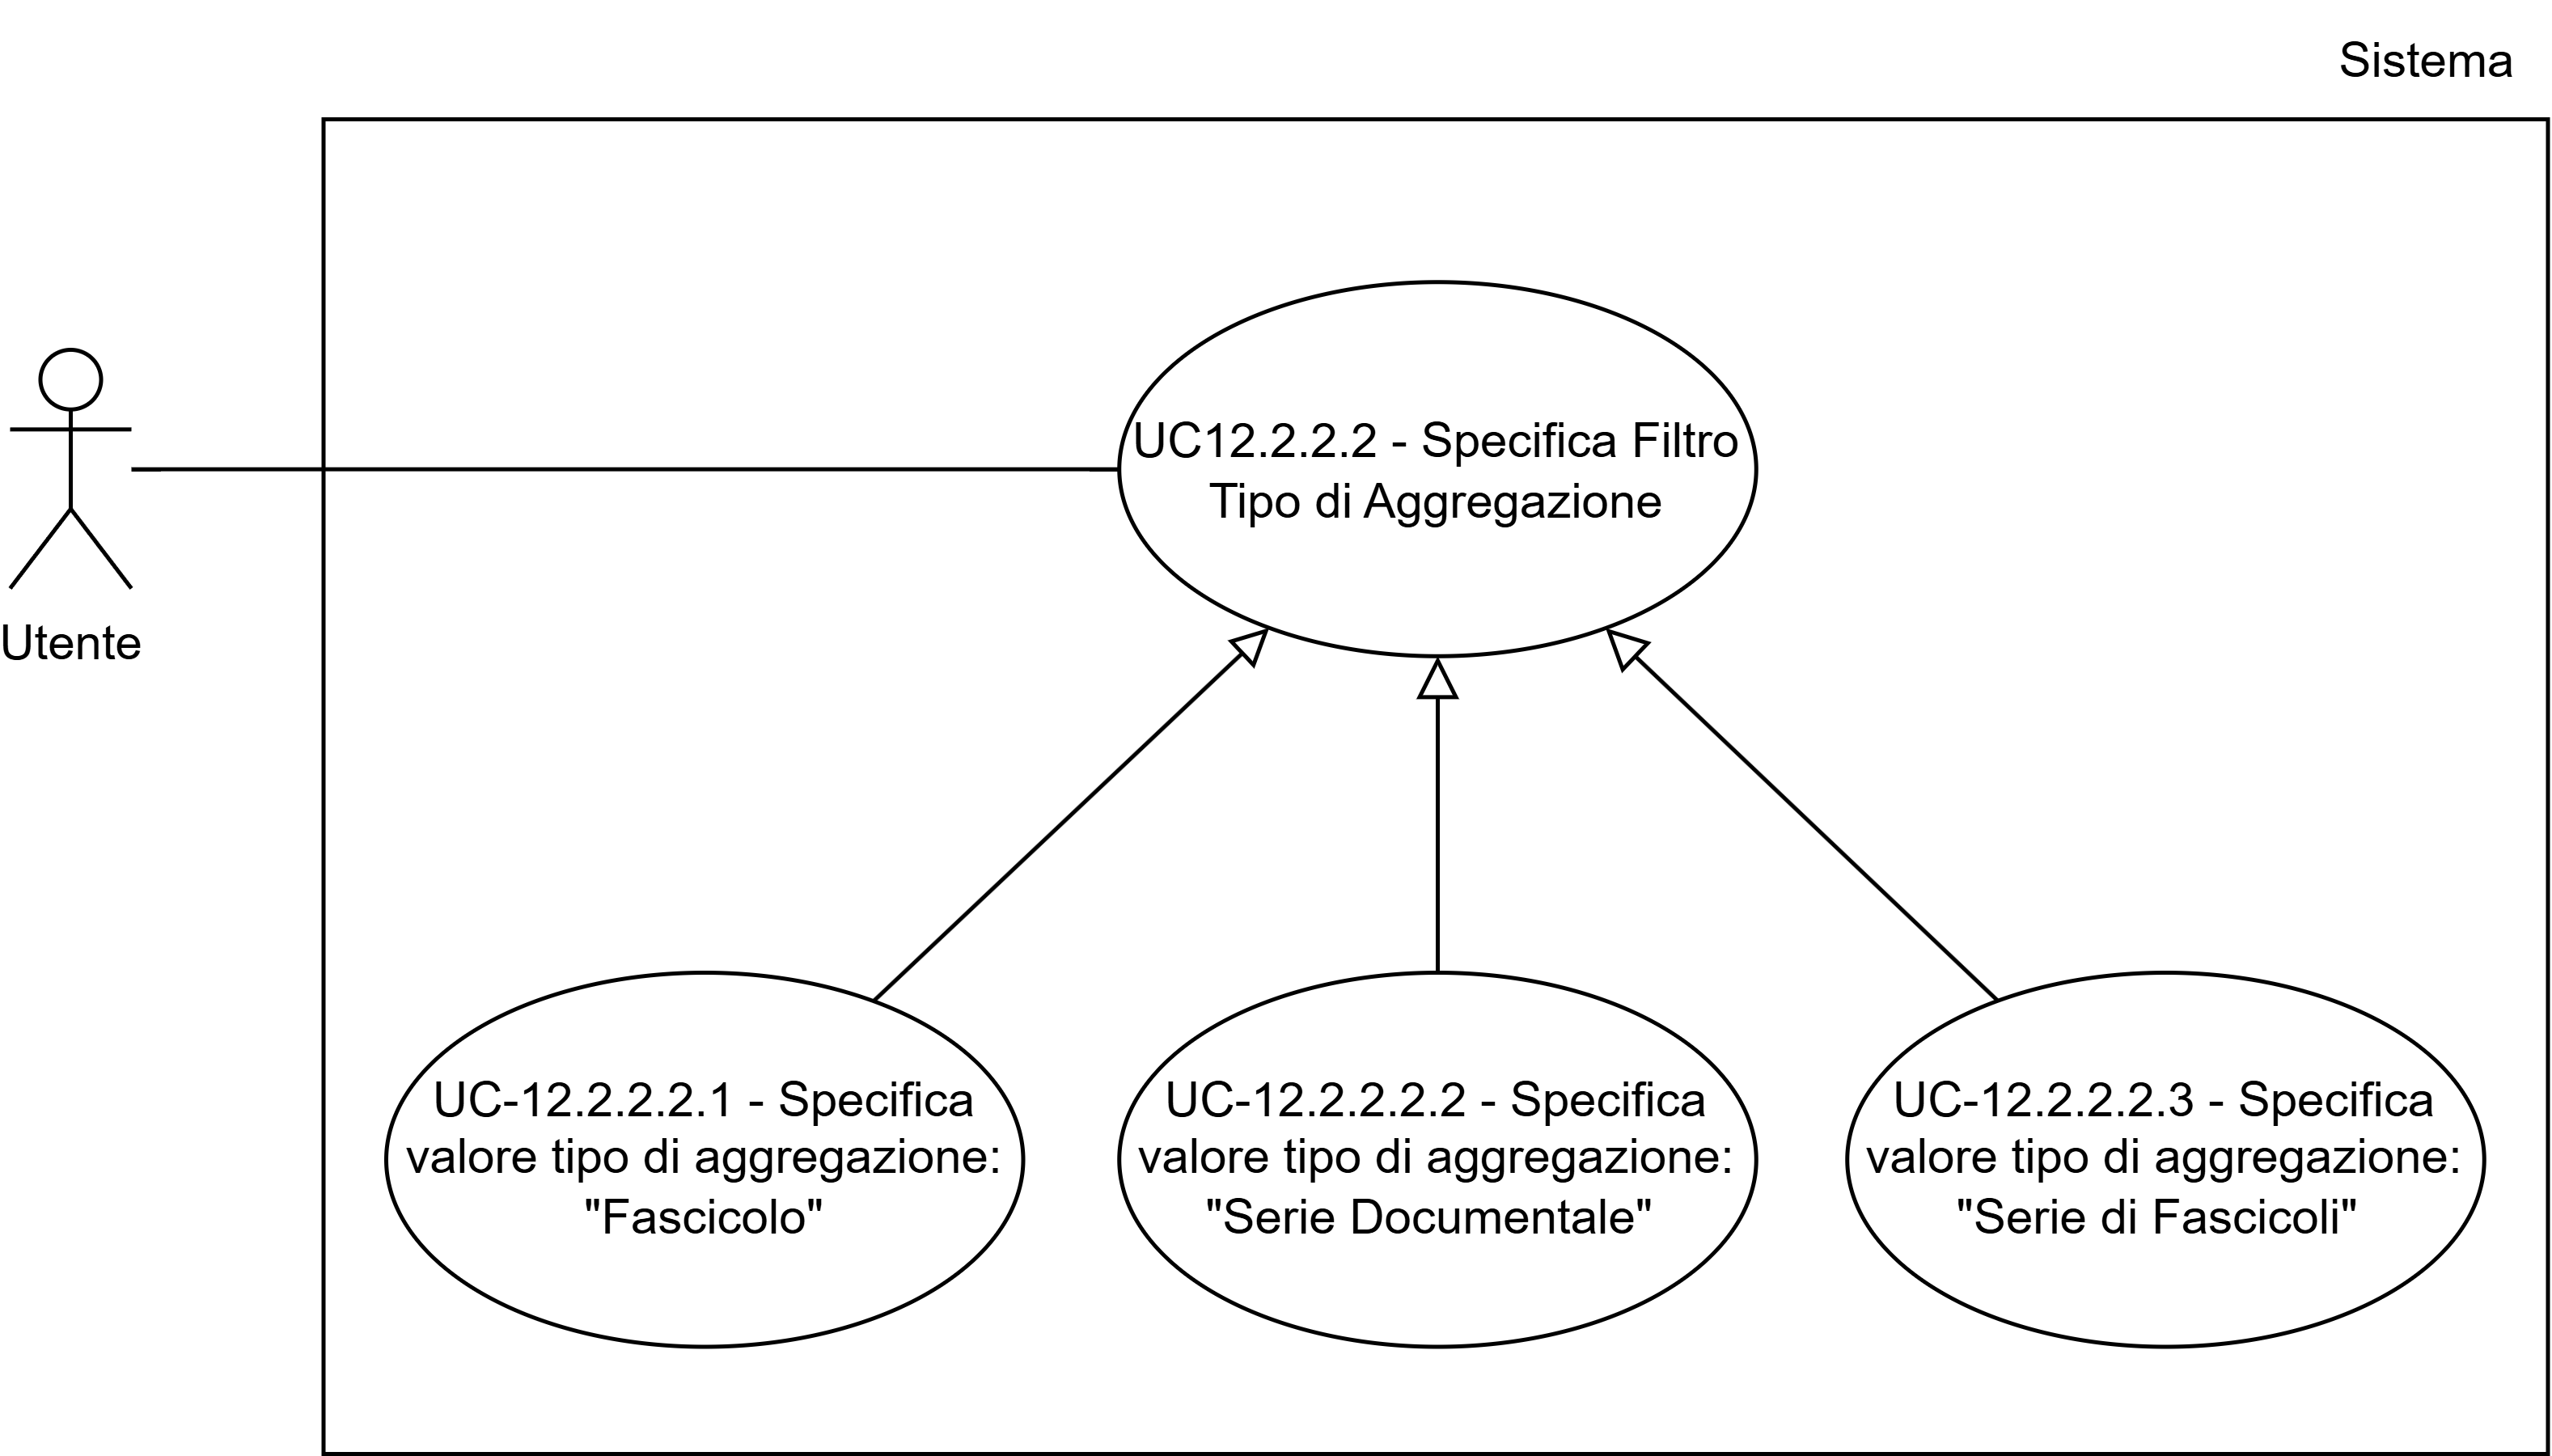
\includegraphics[width=0.8\textwidth]{../../assets/uml/UC12.2.2.2.png}
    \caption{\ref{addTipoAggregazione} - Specifica filtro Tipo di Aggregazione}
    \label{fig:addTipoAggregazione}
\end{figure}
\begin{itemize}
      \item \textbf{Attore Primario}: Utente
      \item \textbf{Precondizioni}: 
      \begin{itemize}
            \item L'Utente ha avviato l'applicazione
            \item L'Utente sta effettuando una ricerca nel DIP con filtri
            \item L'Utente ha specificato come tipo di documento: Aggregazione Documentale
            \item L'utente ha selezionato il filtro Tipo di Aggregazione tra i campi specifici per tipo documentale
      \end{itemize}
      \item \textbf{Postcondizioni}: 
      \begin{itemize}
            \item L'Utente ha specificato i valori del filtro Tipo di Aggregazione
            \item Il filtro Tipo di Aggregazione è parametro per la ricerca con filtri e per la generazione del risultato
      \end{itemize}
      \item \textbf{Flusso Principale}:
      \begin{enumerate}
            \item L'Utente specifica il tipo di aggregazione.
            \item Il sistema imposta questo valore come parametro per la ricerca.
      \end{enumerate}
\end{itemize}

\subdeepusecase{addValoreTipoAggregazioneFascicolo}{Specifica valore tipo di aggregazione: "Fascicolo"}
\begin{itemize}
      \item \textbf{Attore Primario}: Utente
      \item \textbf{Precondizioni}: 
      \begin{itemize}
            \item L'Utente ha avviato l'applicazione
            \item L'Utente sta effettuando una ricerca nel DIP con filtri
            \item L'Utente ha specificato come tipo di documento: Aggregazione Documentale
            \item L'utente ha selezionato il filtro Tipo di Aggregazione tra i campi specifici per tipo documentale
      \end{itemize}
      \item \textbf{Postcondizioni}: Viene selezionato "Fascicolo" come valore del tipo di aggregazione e usato come parametro per la ricerca.
      \item \textbf{Flusso Principale}:
      \begin{enumerate}
            \item L'Utente specifica il valore del tipo di aggregazione: "Fascicolo".
            \item Il sistema imposta questo valore come parametro per la ricerca.
      \end{enumerate}
      \item \textbf{Specializza}: \ref{addTipoAggregazione}
\end{itemize}

\subdeepusecase{addValoreTipoAggregazioneSerieDocumentale}{Specifica valore tipo di aggregazione: "Serie Documentale"}
\begin{itemize}
      \item \textbf{Attore Primario}: Utente
      \item \textbf{Precondizioni}: 
      \begin{itemize}
            \item L'Utente ha avviato l'applicazione
            \item L'Utente sta effettuando una ricerca nel DIP con filtri
            \item L'Utente ha specificato come tipo di documento: Aggregazione Documentale
            \item L'utente ha selezionato il filtro Tipo di Aggregazione tra i campi specifici per tipo documentale
      \end{itemize}
      \item \textbf{Postcondizioni}: Viene selezionato "Serie Documentale" come valore del tipo di aggregazione e usato come parametro per la ricerca.
      \item \textbf{Flusso Principale}:
      \begin{enumerate}
            \item L'Utente specifica il valore del tipo di aggregazione: "Serie Documentale".
            \item Il sistema imposta questo valore come parametro per la ricerca.
      \end{enumerate}
      \item \textbf{Specializza}: \ref{addTipoAggregazione}
\end{itemize}

\subdeepusecase{addValoreTipoAggregazioneSerieFascicoli}{Specifica valore tipo di aggregazione: "Serie di Fascicoli"}
\begin{itemize}
      \item \textbf{Attore Primario}: Utente
      \item \textbf{Precondizioni}: 
      \begin{itemize}
            \item L'Utente ha avviato l'applicazione
            \item L'Utente sta effettuando una ricerca nel DIP con filtri
            \item L'Utente ha specificato come tipo di documento: Aggregazione Documentale
            \item L'utente ha selezionato il filtro Tipo di Aggregazione tra i campi specifici per tipo documentale
      \end{itemize}
      \item \textbf{Postcondizioni}: Viene selezionato "Serie di Fascicoli" come valore del tipo di aggregazione e usato come parametro per la ricerca.
      \item \textbf{Flusso Principale}:
      \begin{enumerate}
            \item L'Utente specifica il valore del tipo di aggregazione: "Serie di Fascicoli".
            \item Il sistema imposta questo valore come parametro per la ricerca.
      \end{enumerate}
      \item \textbf{Specializza}: \ref{addTipoAggregazione}
\end{itemize}

\deepusecase{addIdAggregazione}{Specifica filtro Id dell'Aggregazione}
\begin{figure}[H]
    \centering
    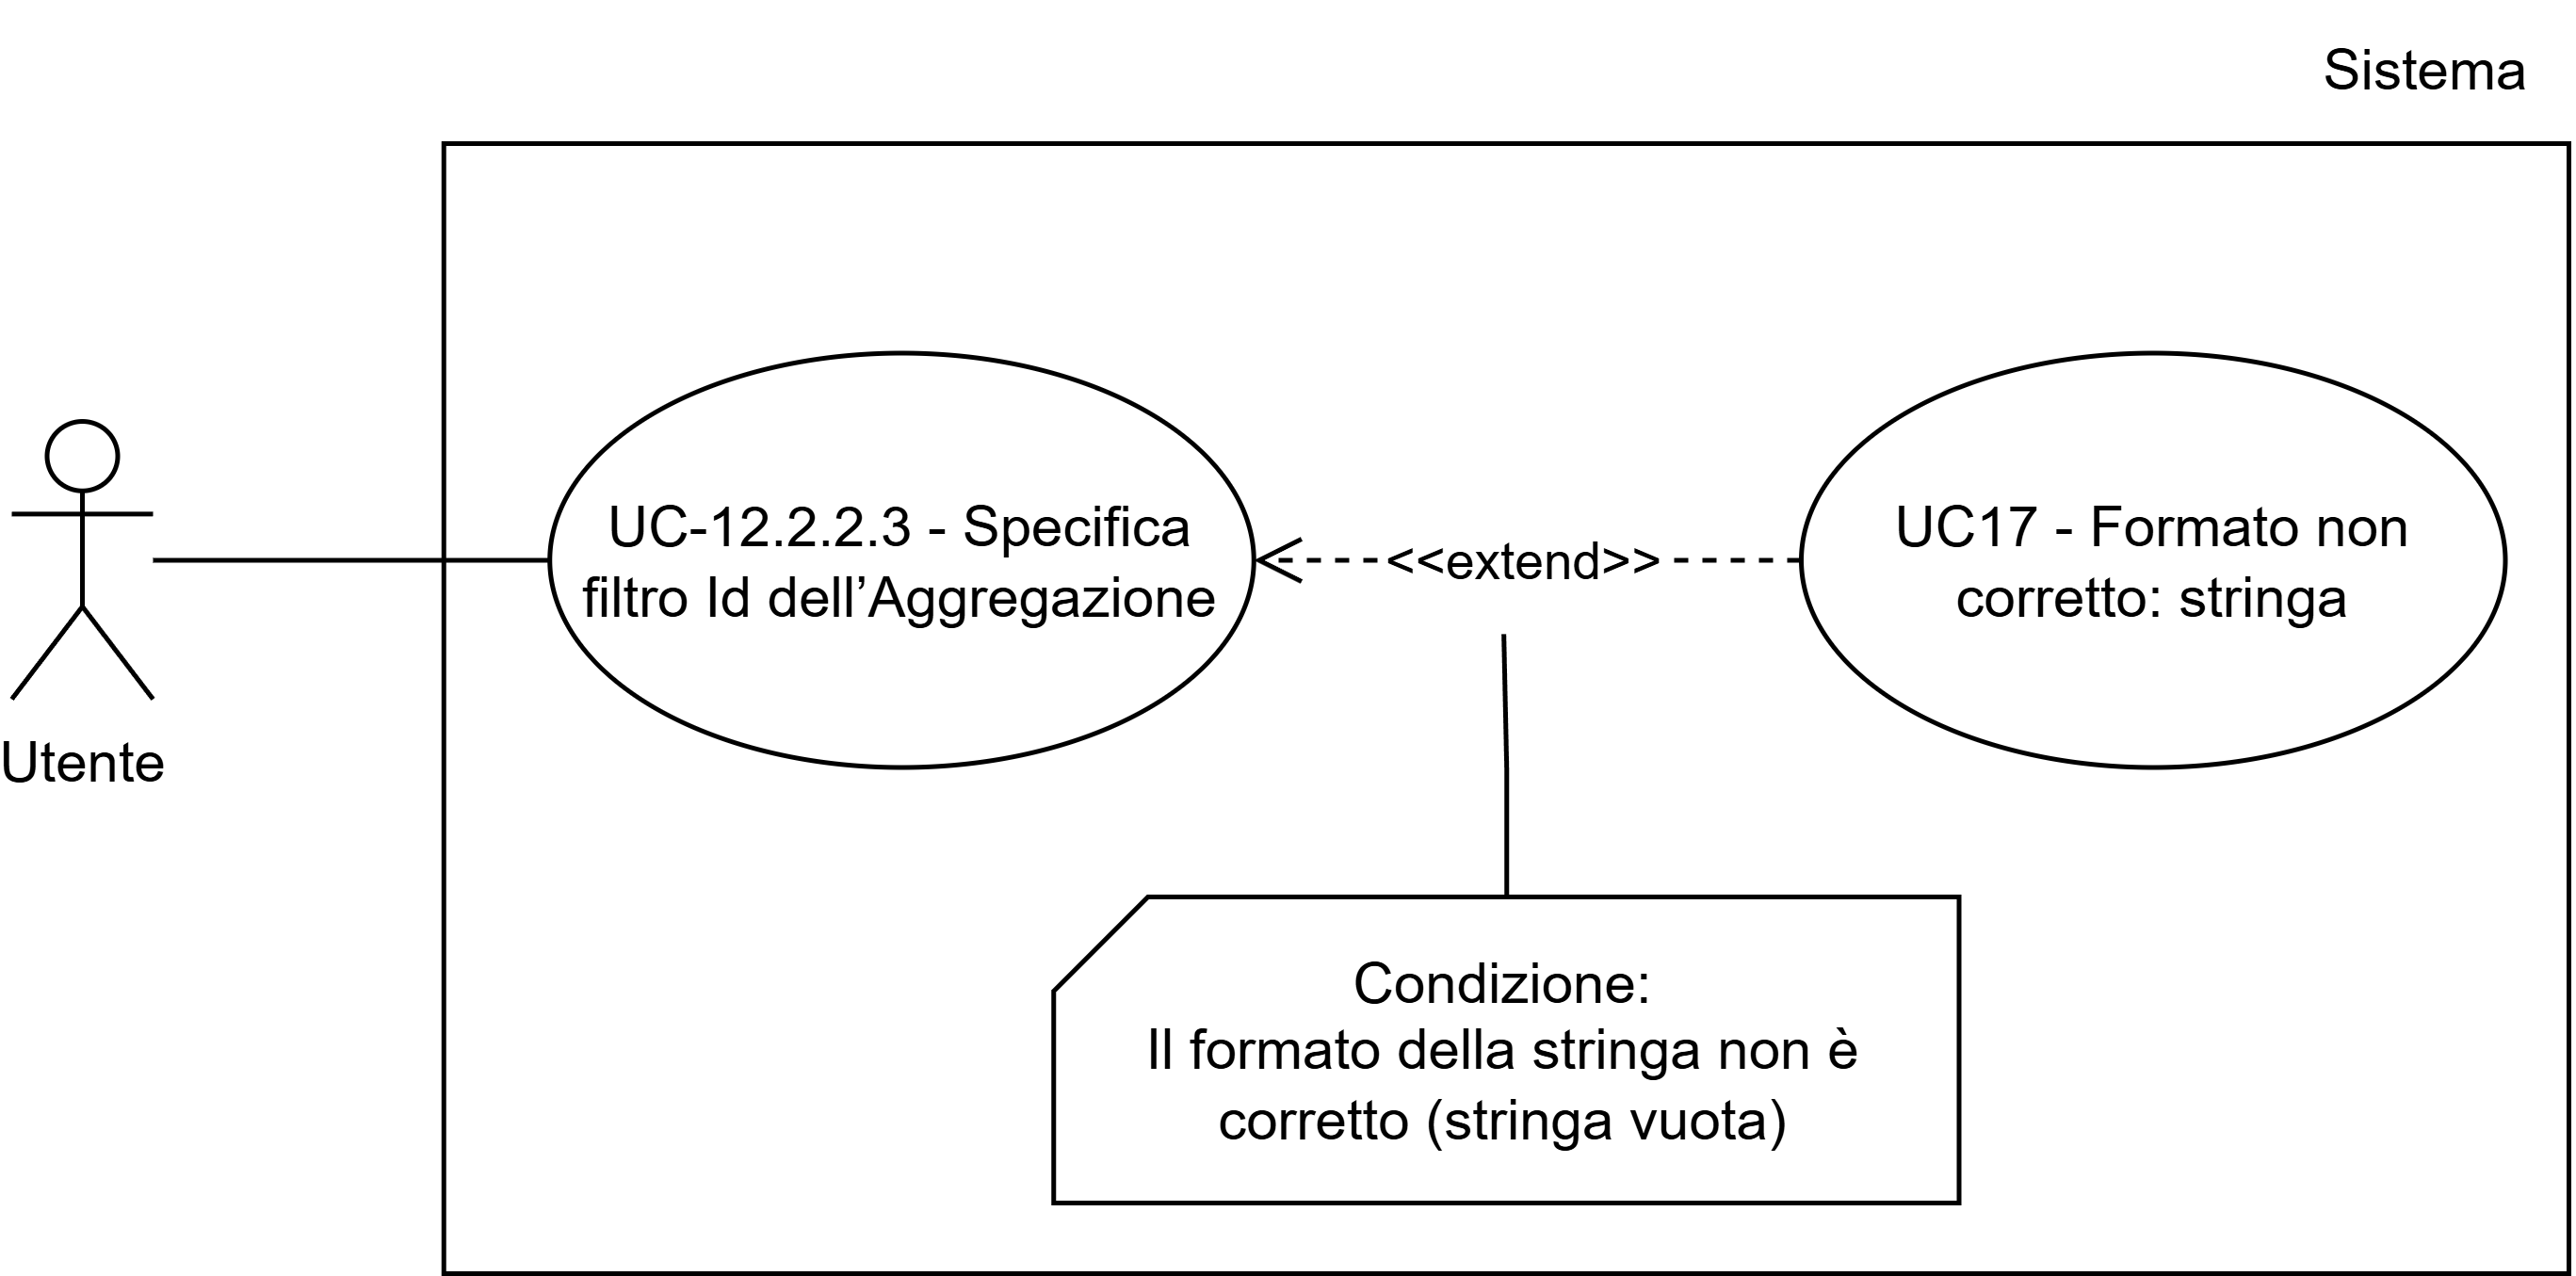
\includegraphics[width=0.8\textwidth]{../../assets/uml/UC12.2.2.3.png}
    \caption{\ref{addIdAggregazione} - Specifica filtro Id dell'Aggregazione}
    \label{fig:addIdAggregazione}
\end{figure}
\begin{itemize}
      \item \textbf{Attore Primario}: Utente
      \item \textbf{Precondizioni}: 
      \begin{itemize}
            \item L'Utente ha avviato l'applicazione
            \item L'Utente sta effettuando una ricerca nel DIP con filtri
            \item L'Utente ha specificato come tipo di documento: Aggregazione Documentale
            \item L'utente ha selezionato il filtro Id dell'Aggregazione tra i campi specifici per tipo documentale
      \end{itemize}
      \item \textbf{Postcondizioni}: \begin{itemize}
            \item L'Utente ha specificato i valori del filtro Id dell'Aggregazione
            \item Il filtro Id dell'Aggregazione è parametro per la ricerca con filtri e per la generazione del risultato
      \end{itemize}
      \item \textbf{Flusso Principale}:
            \begin{enumerate}
                  \item L'Utente specifica l'Id dell'Aggregazione.
                  \item Il sistema imposta questo valore come parametro per la ricerca.
            \end{enumerate}
      \item \textbf{Flusso Alternativo}:
      \begin{itemize}
            \item L'Utente inserisce un identificativo non valido per il filtro Id dell'Aggregazione (stringa vuota) (\ref{formatoNonCorrettoStringa})
      \end{itemize}
      \item \textbf{Estensioni}: \ref{formatoNonCorrettoStringa} Formato non corretto: stringa
\end{itemize}

\deepusecase{addTipologiaFascicolo}{Specifica filtro Tipologia di Fascicolo}
\begin{figure}[H]
    \centering
    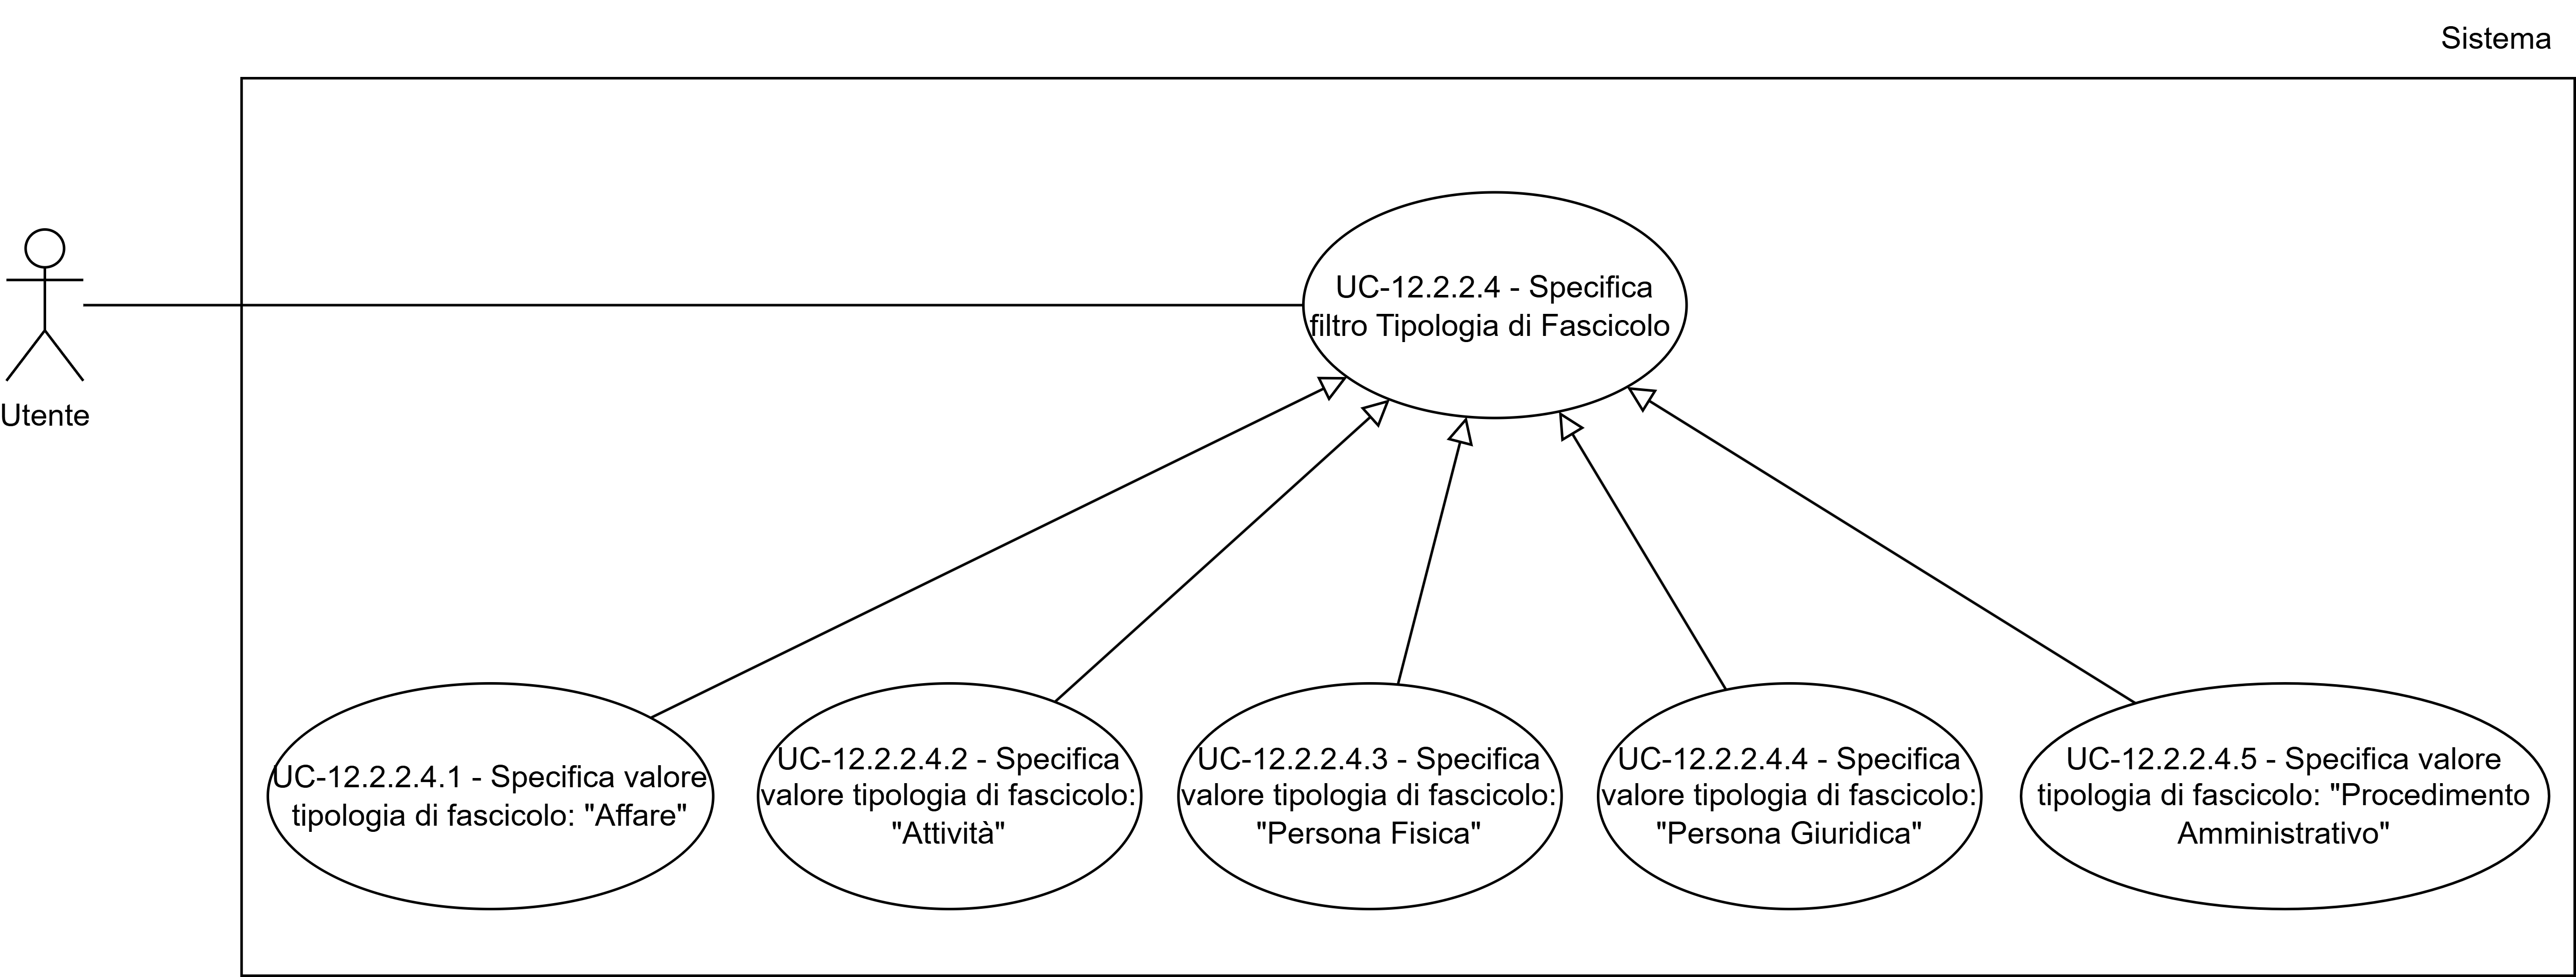
\includegraphics[width=1.1\textwidth]{../../assets/uml/UC12.2.2.4.png}
    \caption{\ref{addTipologiaFascicolo} - Specifica filtro Tipologia di Fascicolo}
    \label{fig:addTipologiaFascicolo}
\end{figure}
\begin{itemize}
      \item \textbf{Attore Primario}: Utente
      \item \textbf{Precondizioni}: 
      \begin{itemize}
            \item L'Utente ha avviato l'applicazione
            \item L'Utente sta effettuando una ricerca nel DIP con filtri
            \item L'Utente ha specificato come tipo di documento: Aggregazione Documentale
            \item L'utente ha selezionato il filtro Tipologia di Fascicolo tra i campi specifici per tipo documentale
      \end{itemize}
      \item \textbf{Postcondizioni}: \begin{itemize}
            \item L'Utente ha specificato i valori del filtro Tipologia di Fascicolo
            \item Il filtro Tipologia di Fascicolo è parametro per la ricerca con filtri e per la generazione del risultato
      \end{itemize}
      \item \textbf{Flusso Principale}:
            \begin{enumerate}
                  \item L'Utente specifica il tipo di fascicolo.
                  \item Il sistema imposta questo valore come parametro per la ricerca.
            \end{enumerate}
\end{itemize}

\subdeepusecase{addValoreTipologiaFascicoloAffare}{Specifica valore tipologia di fascicolo: "Affare"}
\begin{itemize}
      \item \textbf{Attore Primario}: Utente
      \item \textbf{Precondizioni}: 
      \begin{itemize}
            \item L'Utente ha avviato l'applicazione
            \item L'Utente sta effettuando una ricerca nel DIP con filtri
            \item L'Utente ha specificato come tipo di documento: Aggregazione Documentale
            \item L'utente ha selezionato il filtro Tipologia di Fascicolo tra i campi specifici per tipo documentale
      \end{itemize}
      \item \textbf{Postcondizioni}: Viene selezionato "Affare" come valore della tipologia di fascicolo e il filtro è parametro per la ricerca.
      \item \textbf{Flusso Principale}:
            \begin{enumerate}
                  \item L'Utente specifica il valore della tipologia di fascicolo: "Affare".
                  \item Il sistema imposta questo valore come parametro per la ricerca.
            \end{enumerate}
      \item \textbf{Specializza}: \ref{addTipologiaFascicolo}
\end{itemize}

\subdeepusecase{addValoreTipologiaFascicoloAttivita}{Specifica valore tipologia di fascicolo: "Attività"}
\begin{itemize}
      \item \textbf{Attore Primario}: Utente
      \item \textbf{Precondizioni}: 
      \begin{itemize}            
            \item L'Utente ha avviato l'applicazione
            \item L'Utente sta effettuando una ricerca nel DIP con filtri
            \item L'Utente ha specificato come tipo di documento: Aggregazione Documentale
            \item L'utente ha selezionato il filtro Tipologia di Fascicolo tra i campi specifici per tipo documentale
      \end{itemize}
      \item \textbf{Postcondizioni}: Viene selezionato "Attività" come valore della tipologia di fascicolo e il filtro è parametro per la ricerca.
      \item \textbf{Flusso Principale}:
            \begin{enumerate}
                  \item L'Utente specifica il valore della tipologia di fascicolo: "Attività".
                  \item Il sistema imposta questo valore come parametro per la ricerca.
            \end{enumerate}
      \item \textbf{Specializza}: \ref{addTipologiaFascicolo}
\end{itemize}

\subdeepusecase{addValoreTipologiaFascicoloPersonaFisica}{Specifica valore tipologia di fascicolo: "Persona Fisica"}
\begin{itemize}
      \item \textbf{Attore Primario}: Utente
      \item \textbf{Precondizioni}: 
      \begin{itemize}            
            \item L'Utente ha avviato l'applicazione
            \item L'Utente sta effettuando una ricerca nel DIP con filtri
            \item L'Utente ha specificato come tipo di documento: Aggregazione Documentale
            \item L'utente ha selezionato il filtro Tipologia di Fascicolo tra i campi specifici per tipo documentale
      \end{itemize}
      \item \textbf{Postcondizioni}: Viene selezionato "Persona Fisica" come valore della tipologia di fascicolo e il filtro è parametro per la ricerca.
      \item \textbf{Flusso Principale}:
            \begin{enumerate}
                  \item L'Utente specifica il valore della tipologia di fascicolo: "Persona Fisica".
                  \item Il sistema imposta questo valore come parametro per la ricerca.
            \end{enumerate}
      \item \textbf{Specializza}: \ref{addTipologiaFascicolo}
\end{itemize}

\subdeepusecase{addValoreTipologiaFascicoloPersonaGiuridica}{Specifica valore tipologia di fascicolo: "Persona Giuridica"}
\begin{itemize}
      \item \textbf{Attore Primario}: Utente
      \item \textbf{Precondizioni}: 
      \begin{itemize}            
            \item L'Utente ha avviato l'applicazione
            \item L'Utente sta effettuando una ricerca nel DIP con filtri
            \item L'Utente ha specificato come tipo di documento: Aggregazione Documentale
            \item L'utente ha selezionato il filtro Tipologia di Fascicolo tra i campi specifici per tipo documentale
      \end{itemize}
      \item \textbf{Postcondizioni}: Viene selezionato "Persona Giuridica" come valore della tipologia di fascicolo e il filtro è parametro per la ricerca.
      \item \textbf{Flusso Principale}:
            \begin{enumerate}
                  \item L'Utente specifica il valore della tipologia di fascicolo: "Persona Giuridica".
                  \item Il sistema imposta questo valore come parametro per la ricerca.
            \end{enumerate}
      \item \textbf{Specializza}: \ref{addTipologiaFascicolo}
\end{itemize}

\subdeepusecase{addValoreTipologiaFascicoloProcedimentoAmministrativo}{Specifica valore tipologia di fascicolo: "Procedimento Amministrativo"}
\begin{itemize}
      \item \textbf{Attore Primario}: Utente
      \item \textbf{Precondizioni}: 
      \begin{itemize}            
            \item L'Utente ha avviato l'applicazione
            \item L'Utente sta effettuando una ricerca nel DIP con filtri
            \item L'Utente ha specificato come tipo di documento: Aggregazione Documentale
            \item L'utente ha selezionato il filtro Tipologia di Fascicolo tra i campi specifici per tipo documentale
      \end{itemize}
      \item \textbf{Postcondizioni}: Viene selezionato "Procedimento Amministrativo" come valore della tipologia di fascicolo e il filtro è parametro per la ricerca.
      \item \textbf{Flusso Principale}:
            \begin{enumerate}
                  \item L'Utente specifica il valore della tipologia di fascicolo: "Procedimento Amministrativo".
                  \item Il sistema imposta questo valore come parametro per la ricerca.
            \end{enumerate}
      \item \textbf{Specializza}: \ref{addTipologiaFascicolo}
\end{itemize}

\deepusecase{addIdAggregazionePrimario}{Specifica filtro Id Aggregazione Primario}
\begin{figure}[H]
    \centering
    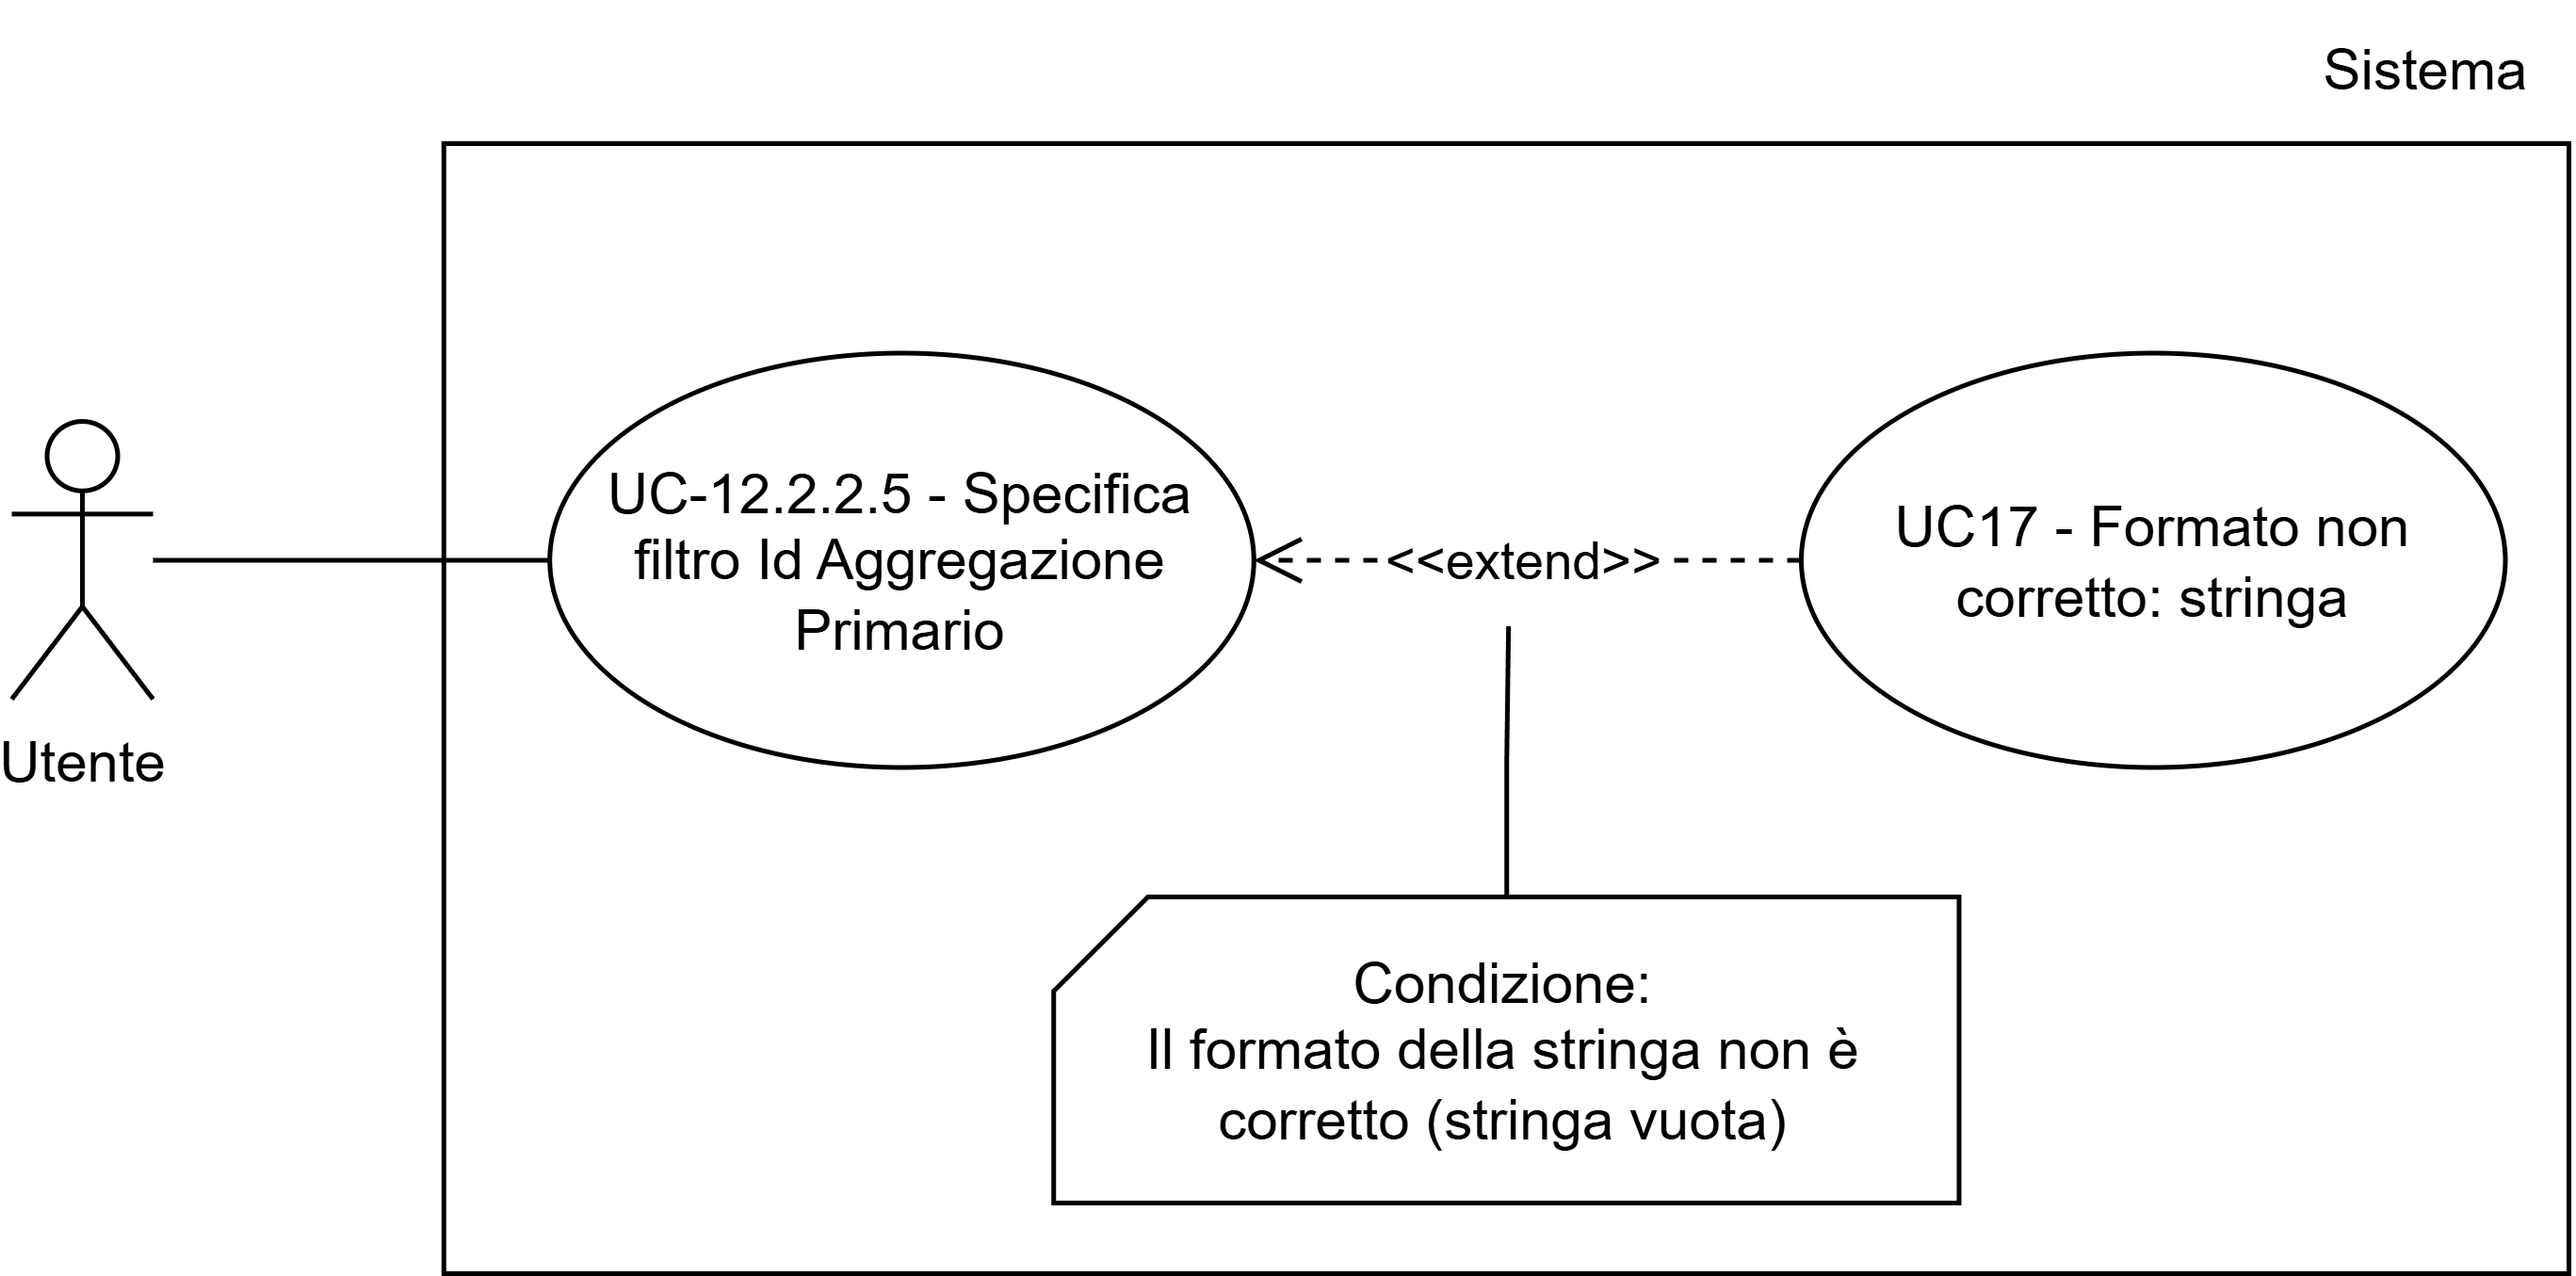
\includegraphics[width=0.8\textwidth]{../../assets/uml/UC12.2.2.5.png}
    \caption{\ref{addIdAggregazionePrimario} - Specifica filtro Id dell'Aggregazione Primario}
    \label{fig:addIdAggregazionePrimario}
\end{figure}
\begin{itemize}
      \item \textbf{Attore Primario}: Utente
      \item \textbf{Precondizioni}: 
      \begin{itemize}
            \item L'Utente ha avviato l'applicazione
            \item L'Utente sta effettuando una ricerca nel DIP con filtri
            \item L'Utente ha specificato come tipo di documento: Aggregazione Documentale
            \item L'utente ha selezionato il filtro Id dell'Aggregazione Primario tra i campi specifici per tipo documentale
      \end{itemize}
      \item \textbf{Postcondizioni}: \begin{itemize}
            \item L'Utente ha specificato i valori del filtro Id dell'Aggregazione Primario
            \item Il filtro Id dell'Aggregazione Primario è parametro per la ricerca con filtri e per la generazione del risultato
      \end{itemize}
      \item \textbf{Flusso Principale}:
            \begin{enumerate}
                  \item L'Utente specifica l'Id Primario dell'Aggregazione.
                  \item Il sistema imposta questo valore come parametro per la ricerca.
            \end{enumerate}
      \item \textbf{Flusso Alternativo}:
      \begin{itemize}
            \item L'Utente inserisce un Id Primario non valido per il filtro Id dell'Aggregazione Primario (stringa vuota) (\ref{formatoNonCorrettoStringa})
      \end{itemize}
      \item \textbf{Estensioni}: \ref{formatoNonCorrettoStringa} Formato non corretto: stringa
\end{itemize}

\deepusecase{addDataApertura}{Specifica filtro Data Apertura}
\begin{figure}[H]
    \centering
    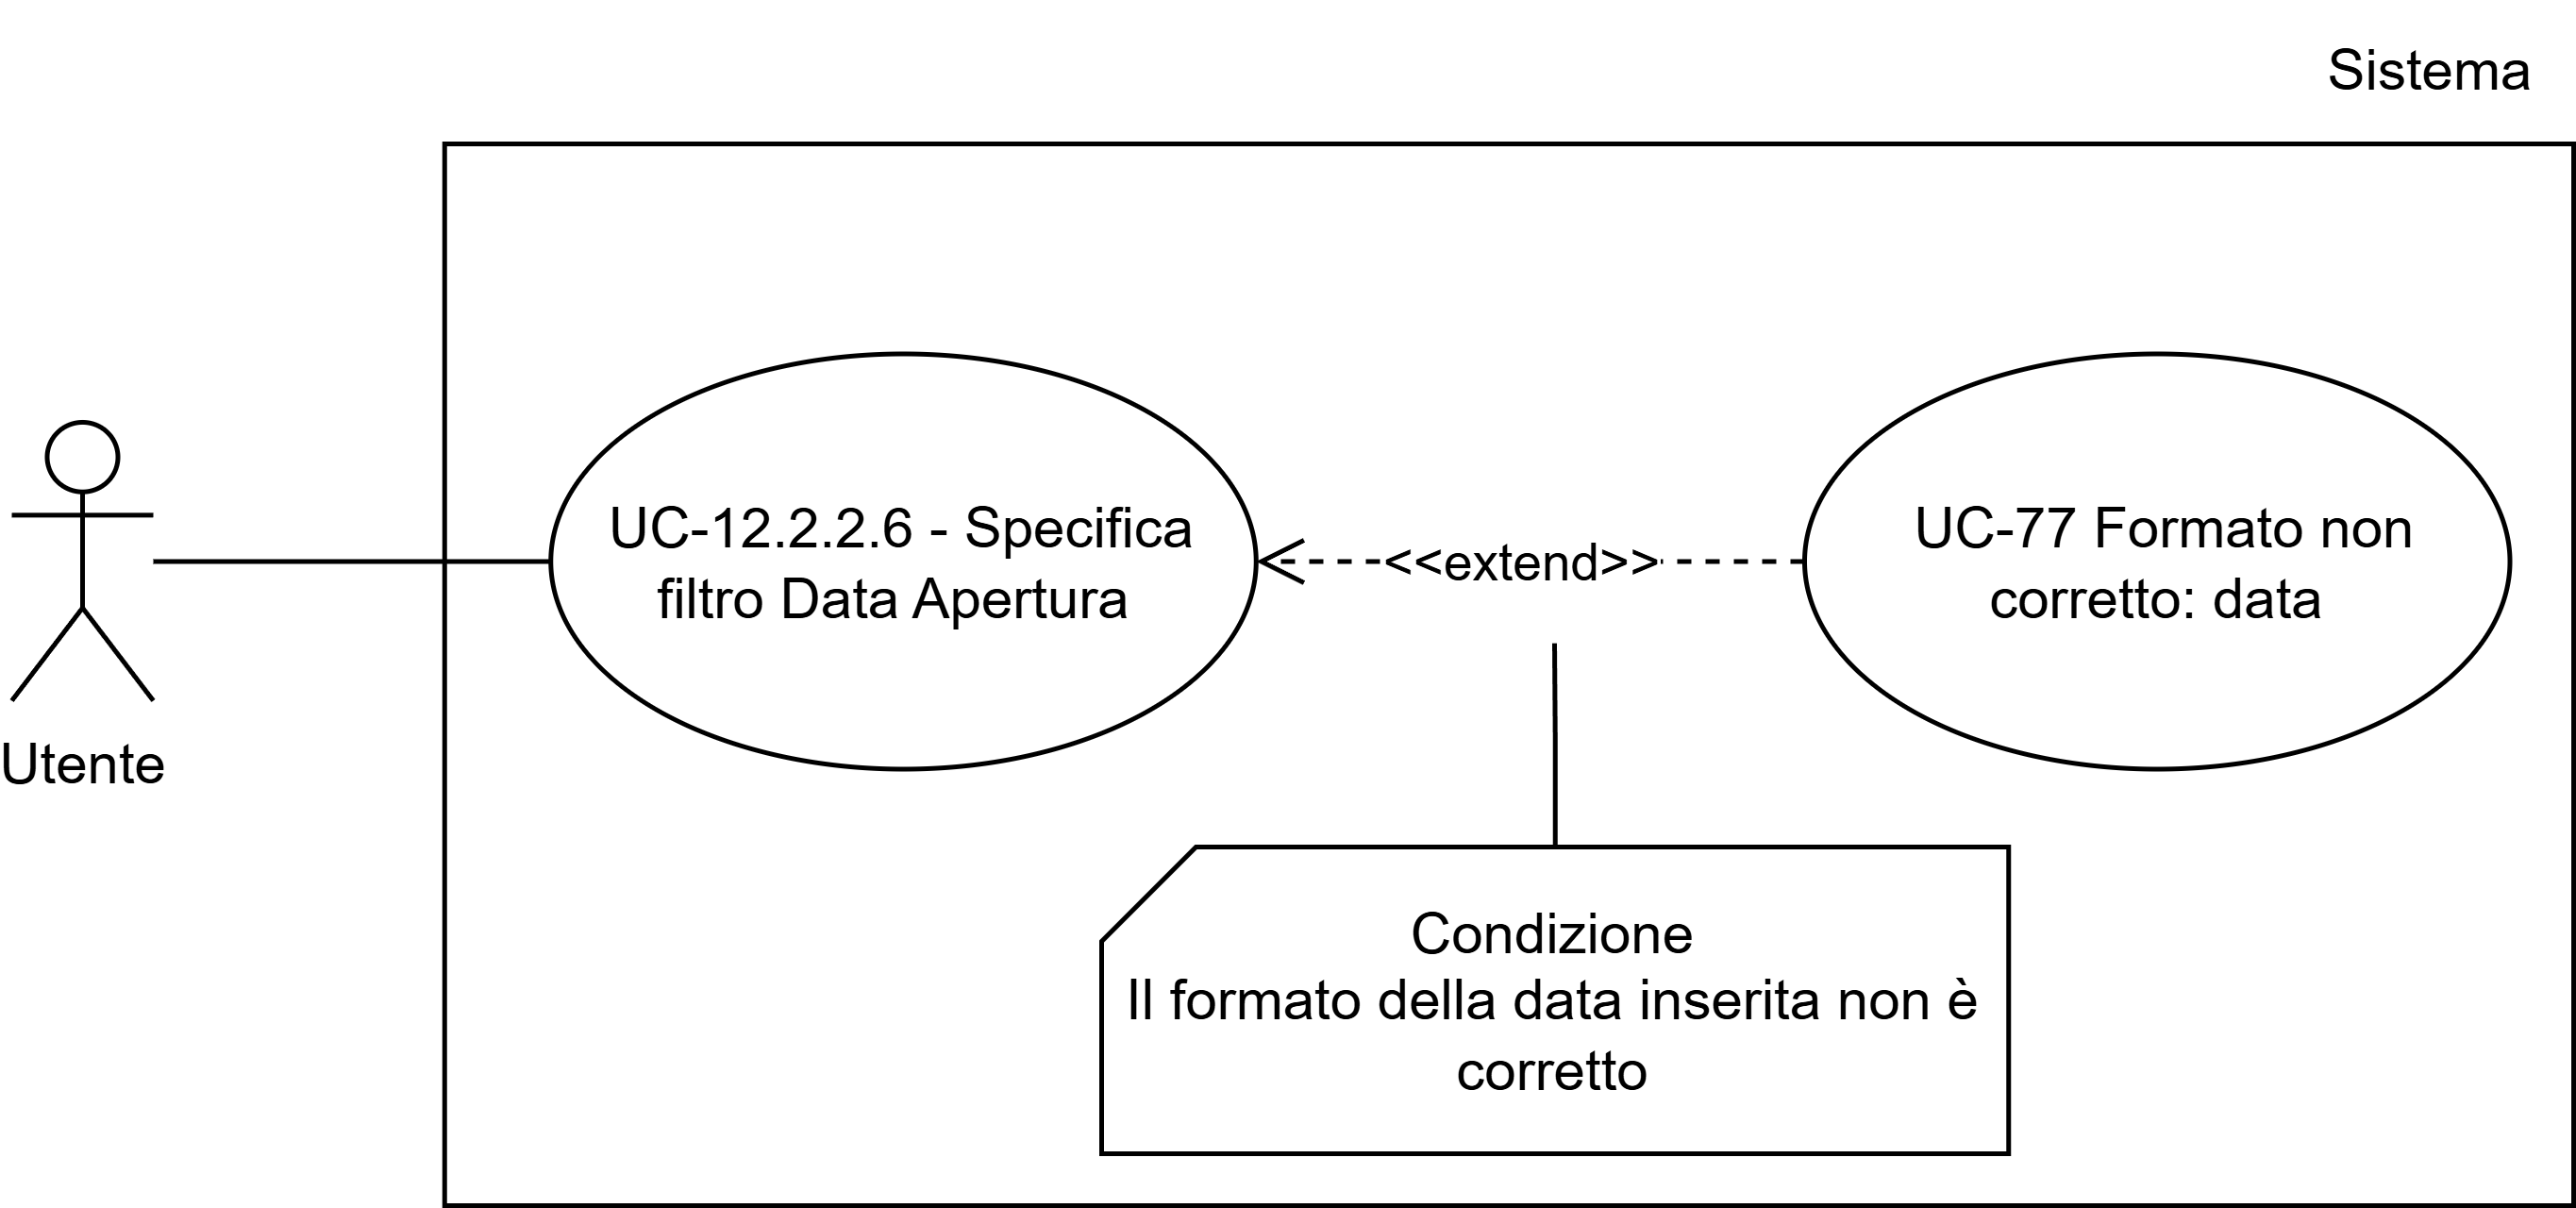
\includegraphics[width=0.8\textwidth]{../../assets/uml/UC12.2.2.6.png}
    \caption{\ref{addDataApertura} - Specifica filtro Data Apertura}
    \label{fig:addDataApertura}
\end{figure}
\begin{itemize}
      \item \textbf{Attore Primario}: Utente
      \item \textbf{Precondizioni}: 
      \begin{itemize}
            \item L'Utente ha avviato l'applicazione
            \item L'Utente sta effettuando una ricerca nel DIP con filtri
            \item L'Utente ha specificato come tipo di documento: Aggregazione Documentale
            \item L'utente ha selezionato il filtro Data di Apertura tra i campi specifici per tipo documentale
      \end{itemize}
      \item \textbf{Postcondizioni}: \begin{itemize}
            \item L'Utente ha specificato i valori del filtro Data di Apertura
            \item Il filtro Data di Apertura è parametro per la ricerca con filtri e per la generazione del risultato
      \end{itemize}
      \item \textbf{Flusso Principale}:
            \begin{enumerate}
                  \item L'Utente specifica la Data di Apertura.
                  \item Il sistema imposta questo valore come parametro per la ricerca.
            \end{enumerate}
      \item \textbf{Flusso Alternativo}:
      \begin{itemize}
            \item L'Utente inserisce una data non valida per il filtro Data di Apertura (formato data errato) (\ref{formatoNonCorrettoData})
      \end{itemize}
      \item \textbf{Estensioni}: \ref{formatoNonCorrettoData} Formato non corretto: data
\end{itemize}

\deepusecase{addDataChiusura}{Specifica filtro Data Chiusura}
\begin{figure}[H]
    \centering
    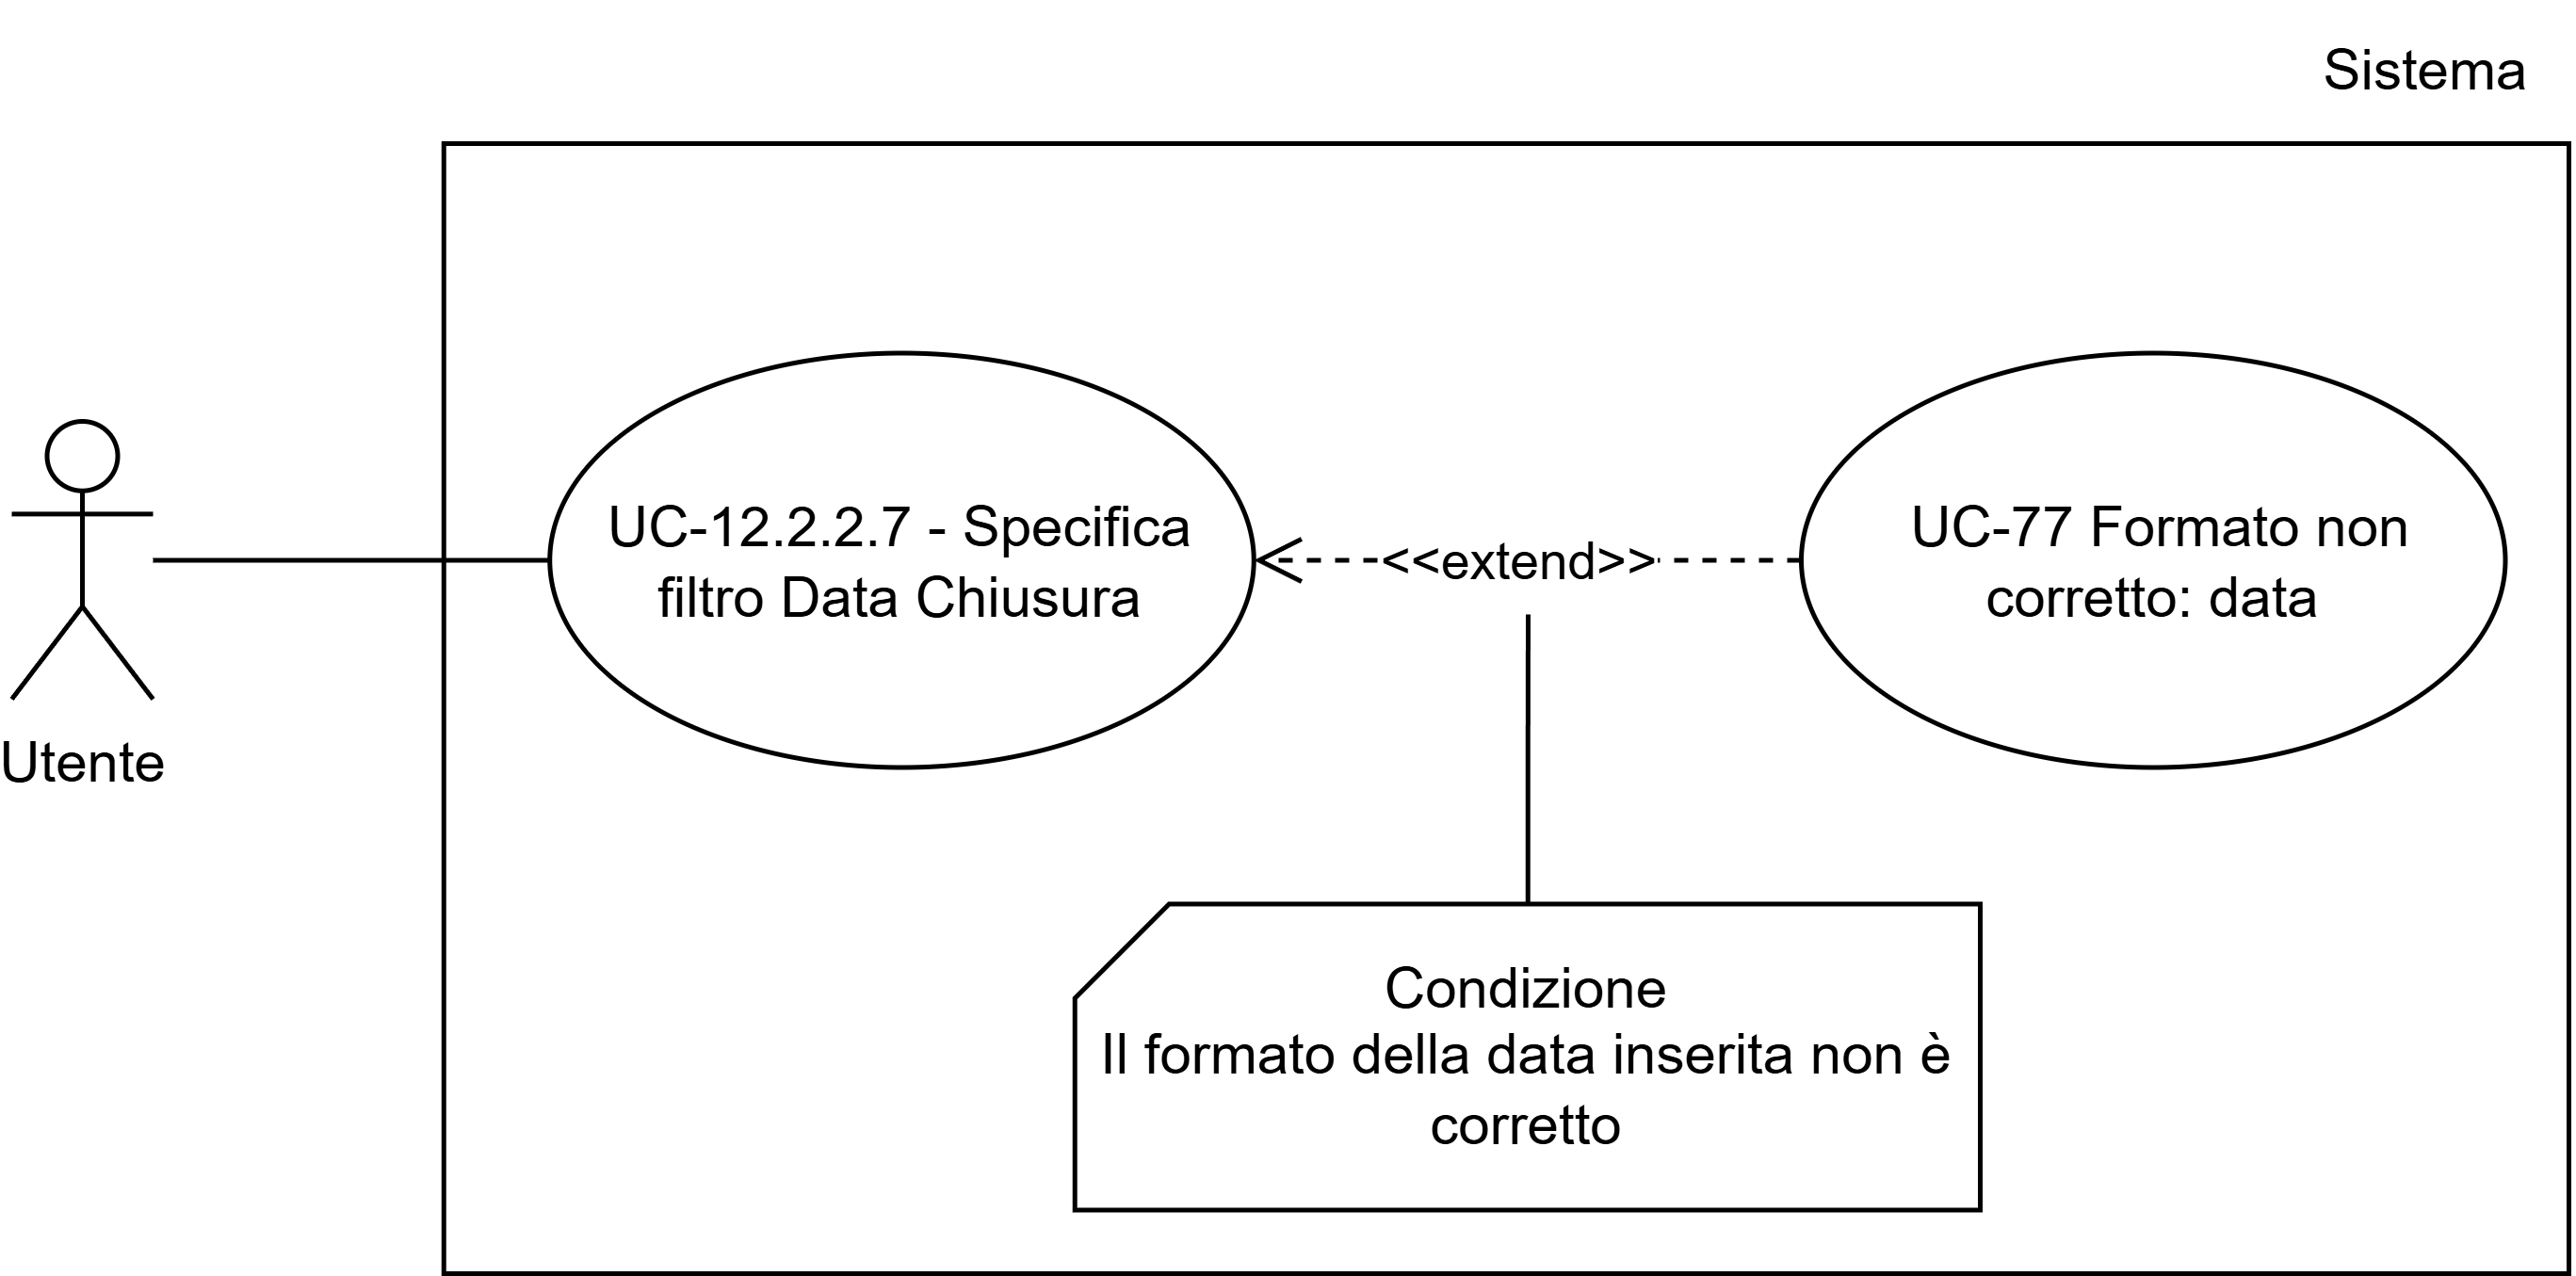
\includegraphics[width=0.8\textwidth]{../../assets/uml/UC12.2.2.7.png}
    \caption{\ref{addDataChiusura} - Specifica filtro Data Chiusura}
    \label{fig:addDataChiusura}
\end{figure}
\begin{itemize}
      \item \textbf{Attore Primario}: Utente
      \item \textbf{Precondizioni}: 
      \begin{itemize}
            \item L'Utente ha avviato l'applicazione
            \item L'Utente sta effettuando una ricerca nel DIP con filtri
            \item L'Utente ha specificato come tipo di documento: Aggregazione Documentale
            \item L'utente ha selezionato il filtro Data di Chiusura tra i campi specifici per tipo documentale
      \end{itemize}
      \item \textbf{Postcondizioni}: \begin{itemize}
            \item L'Utente ha specificato i valori del filtro Data di Chiusura
            \item Il filtro Data di Chiusura è parametro per la ricerca con filtri e per la generazione del risultato
      \end{itemize}
      \item \textbf{Flusso Principale}:
            \begin{enumerate}
                  \item L'Utente specifica la Data di Chiusura.
                  \item Il sistema imposta questo valore come parametro per la ricerca.
            \end{enumerate}
      \item \textbf{Flusso Alternativo}:
      \begin{itemize}
            \item L'Utente inserisce una data non valida per il filtro Data di Chiusura (formato data errato) (\ref{formatoNonCorrettoData})
      \end{itemize}
      \item \textbf{Estensioni}: \ref{formatoNonCorrettoData} Formato non corretto: data
\end{itemize}

\deepusecase{addProcedimentoAmministrativo}{Specifica filtro Procedimento Amministrativo}
\begin{figure}[H]
    \centering
    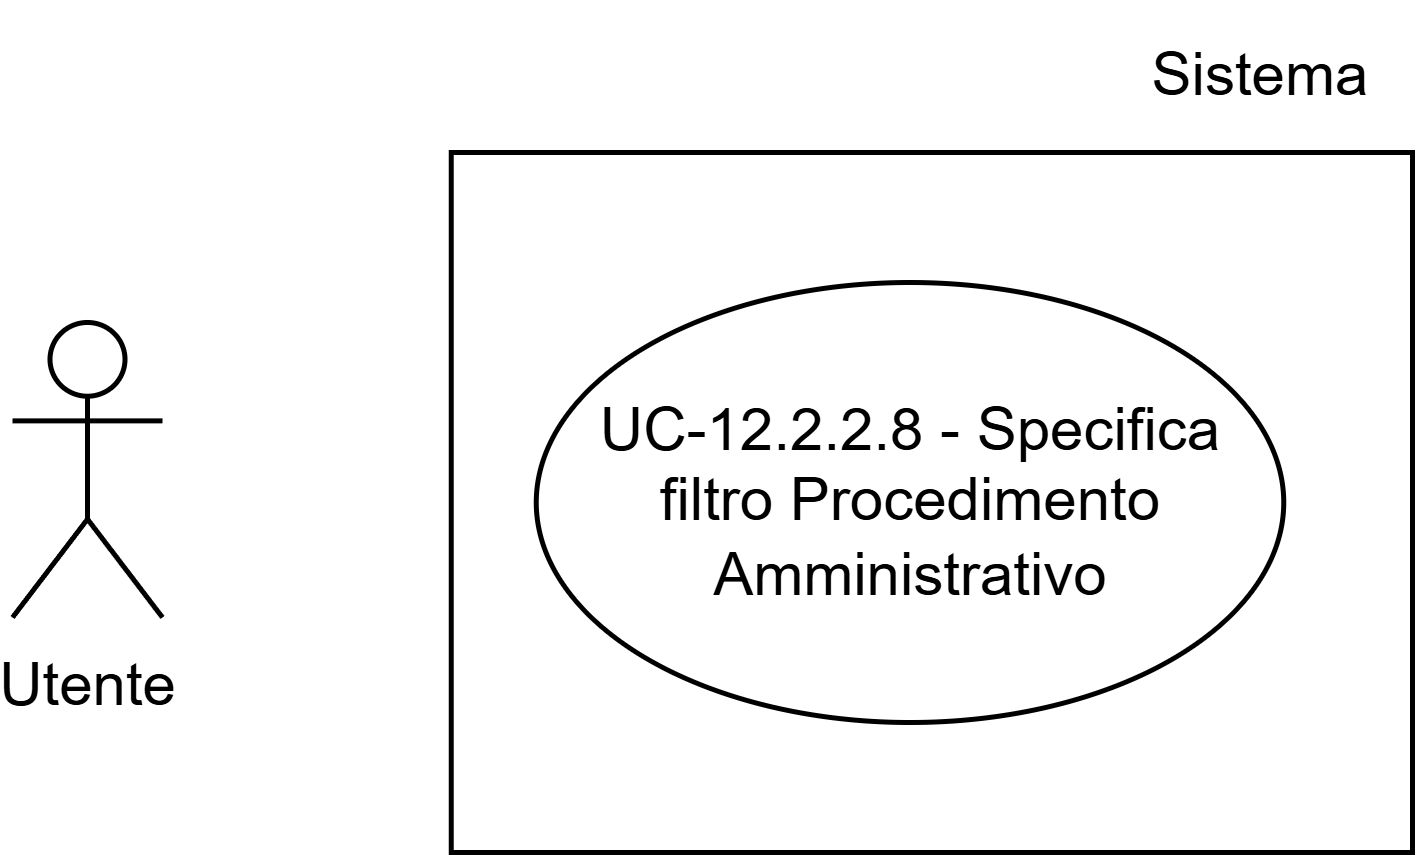
\includegraphics[width=0.8\textwidth]{../../assets/uml/UC12.2.2.8.png}
    \caption{\ref{addProcedimentoAmministrativo} - Specifica filtro Procedimento Amministrativo}
    \label{fig:addProcedimentoAmministrativo}
\end{figure}
\begin{itemize}
      \item \textbf{Attore Primario}: Utente
      \item \textbf{Precondizioni}: 
      \begin{itemize}
            \item L'Utente ha avviato l'applicazione
            \item L'Utente sta effettuando una ricerca nel DIP con filtri
            \item L'Utente ha specificato come tipo di documento: Aggregazione Documentale
            \item L'utente ha selezionato il filtro Procedimento Amministrativo tra i campi specifici per tipo documentale
      \end{itemize}
      \item \textbf{Postcondizioni}: 
      \begin{itemize}
            \item L'Utente ha specificato i valori del filtro Procedimento Amministrativo
            \item Il filtro Procedimento Amministrativo è parametro per la ricerca con filtri e per la generazione del risultato
      \end{itemize}
      \item \textbf{Flusso Principale}:
      \begin{enumerate}
            \item L'Utente specifica la Materia, Argomento e Struttura per i procedimenti.
            \item L'Utente specifica il Procedimento come denominazione.
            \item L'Utente specifica il Catalogo dei Procedimenti come URI di pubblicazione del catalogo.
            \item L'Utente aggiunge una o più Fasi (\ref{addFasiProcedimentoAmministrativo})(0...n).
            \item Il sistema imposta i valori del filtro come parametri di ricerca.
      \end{enumerate}
      \item \textbf{Inclusioni}: 
      \begin{itemize}
            \item \ref{addFasiProcedimentoAmministrativo} Aggiunta Fase del Procedimento Amministrativo
            \item \ref{addValoreMateriaArgomentoStrutturaProcedimentoAmministrativo} Specifica valore Materia/Argomento/Struttura per filtro Procedimento Amministrativo
            \item \ref{addValoreDenominazioneProcedimentoAmministrativo} Specifica valore Denominazione per filtro Procedimento Amministrativo
            \item \ref{addValoreURICatalogoProcedimenti} Specifica valore URI Catalogo per filtro Procedimento Amministrativo
      \end{itemize}
\end{itemize}
\begin{figure}[H]
      \centering
      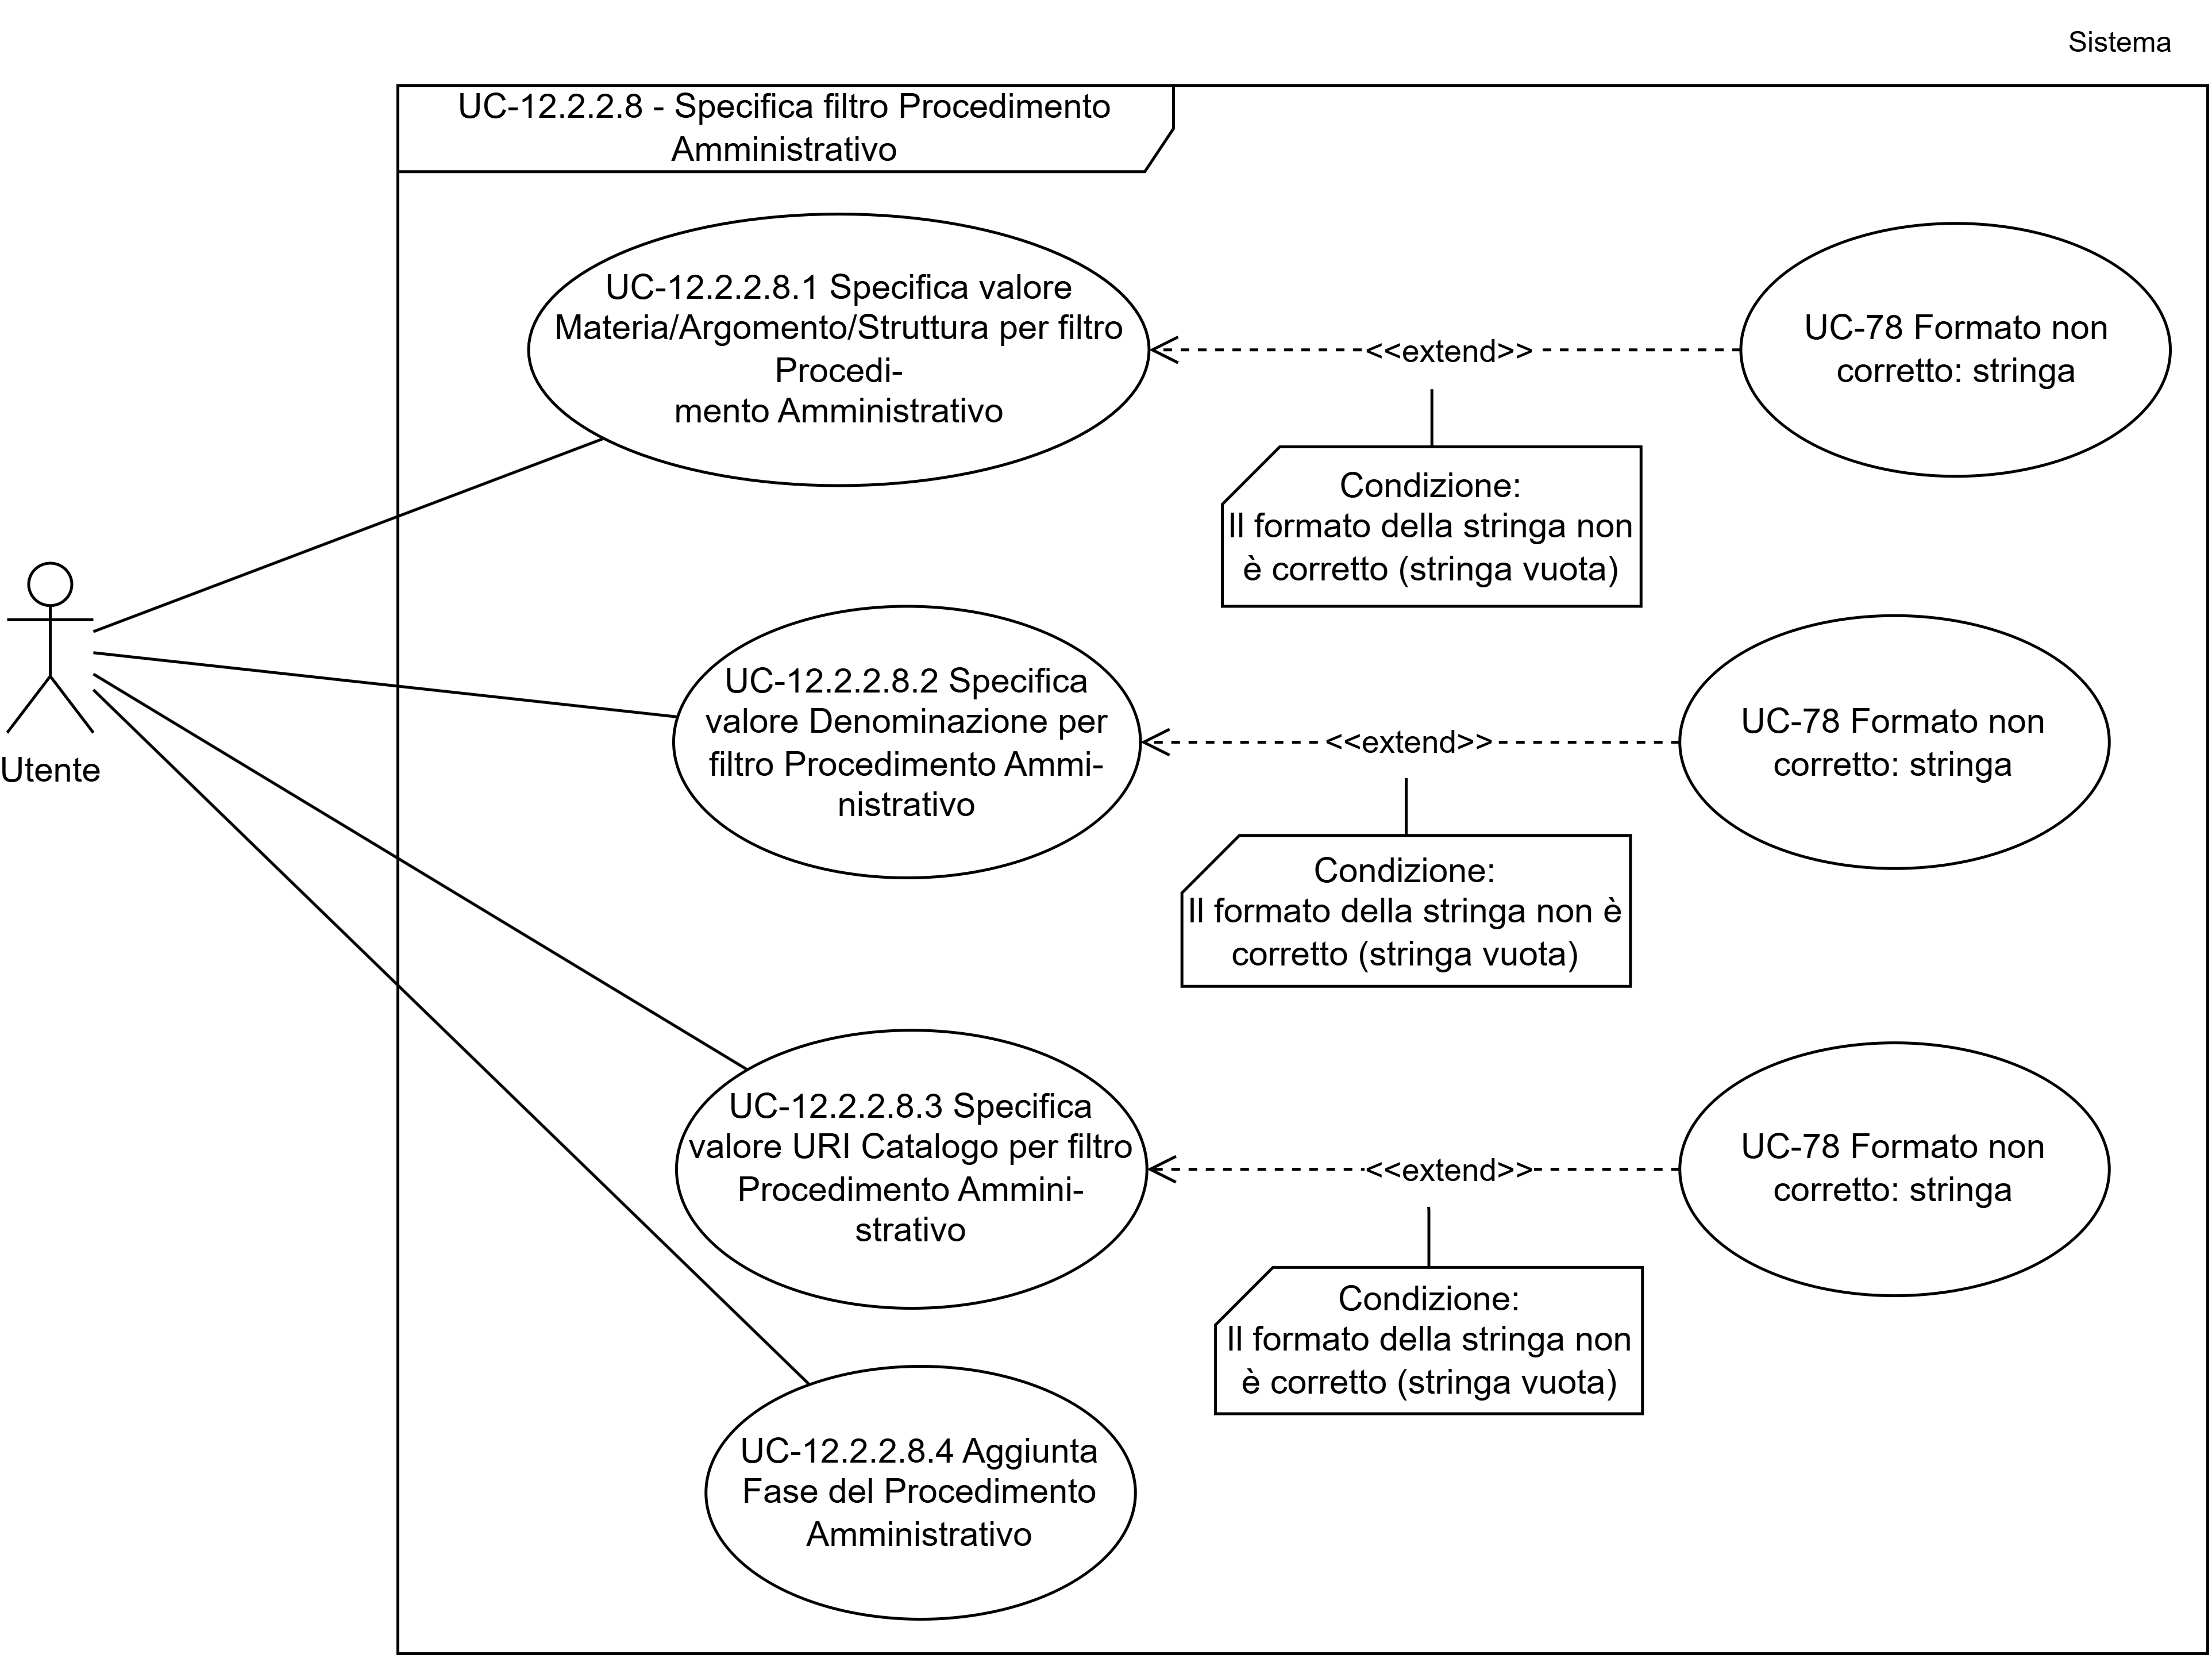
\includegraphics[width=1\textwidth]{../../assets/uml/UC12.2.2.8INC.png}
      \caption{Inclusioni \ref{addProcedimentoAmministrativo} - Specifica filtro Procedimento Amministrativo}
      \label{fig:inclusioniSpecificaFiltriProcedimentoAmministrativo}
\end{figure}

\subdeepusecase{addValoreMateriaArgomentoStrutturaProcedimentoAmministrativo}{Specifica valore Materia/Argomento/Struttura per filtro Procedimento Amministrativo}
\begin{itemize}
      \item \textbf{Attore Primario}: Utente
      \item \textbf{Precondizioni}: 
      \begin{itemize}            
            \item L'Utente ha avviato l'applicazione
            \item L'Utente sta effettuando una ricerca nel DIP con filtri
            \item L'Utente ha specificato come tipo di documento: Aggregazione Documentale
            \item L'utente ha selezionato il filtro Procedimento Amministrativo tra i campi specifici per tipo documentale
      \end{itemize}
      \item \textbf{Postcondizioni}: Viene specificata la Materia/Argomento/Struttura per il filtro Procedimento Amministrativo e utilizzata per la generazione del risultato.
      \item \textbf{Flusso Principale}:
      \begin{enumerate}
            \item L'Utente specifica la Materia/Argomento/Struttura per il filtro Procedimento Amministrativo.
            \item Il sistema imposta questo valore come parametro per la ricerca.
      \end{enumerate}
      \item \textbf{Flusso Alternativo}:
      \begin{itemize}
            \item L'Utente inserisce un valore non valido per il filtro Materia, Argomento e Struttura del Procedimento Amministrativo (stringa vuota) (\ref{formatoNonCorrettoStringa})
      \end{itemize}
      \item \textbf{Estensioni}: \ref{formatoNonCorrettoStringa} Formato non corretto: stringa
\end{itemize}

\subdeepusecase{addValoreDenominazioneProcedimentoAmministrativo}{Specifica valore Denominazione per filtro Procedimento Amministrativo}
\begin{itemize}
      \item \textbf{Attore Primario}: Utente
      \item \textbf{Precondizioni}: 
      \begin{itemize}            
            \item L'Utente ha avviato l'applicazione
            \item L'Utente sta effettuando una ricerca nel DIP con filtri
            \item L'Utente ha specificato come tipo di documento: Aggregazione Documentale
            \item L'utente ha selezionato il filtro Procedimento Amministrativo tra i campi specifici per tipo documentale
      \end{itemize}
      \item \textbf{Postcondizioni}: Viene specificata la Denominazione per il filtro Procedimento Amministrativo e utilizzata per la generazione del risultato.
      \item \textbf{Flusso Principale}:
      \begin{enumerate}
            \item L'Utente specifica la Denominazione per il filtro Procedimento Amministrativo.
            \item Il sistema imposta questo valore come parametro per la ricerca.
      \end{enumerate}
      \item \textbf{Flusso Alternativo}:
      \begin{itemize}
            \item L'Utente inserisce un valore non valido per il filtro Denominazione del Procedimento Amministrativo (stringa vuota) (\ref{formatoNonCorrettoStringa})
      \end{itemize}
      \item \textbf{Estensioni}: \ref{formatoNonCorrettoStringa} Formato non corretto: stringa
\end{itemize}

\subdeepusecase{addValoreURICatalogoProcedimenti}{Specifica valore URI Catalogo per filtro Procedimento Amministrativo}
\begin{itemize}
      \item \textbf{Attore Primario}: Utente
      \item \textbf{Precondizioni}: 
      \begin{itemize}            
            \item L'Utente ha avviato l'applicazione
            \item L'Utente sta effettuando una ricerca nel DIP con filtri
            \item L'Utente ha specificato come tipo di documento: Aggregazione Documentale
            \item L'utente ha selezionato il filtro Procedimento Amministrativo tra i campi specifici per tipo documentale
      \end{itemize}
      \item \textbf{Postcondizioni}: Viene specificata la URI del Catalogo dei Procedimenti per il filtro Procedimento Amministrativo e utilizzata per la generazione del risultato.
      \item \textbf{Flusso Principale}:
      \begin{enumerate}
            \item L'Utente specifica la URI del Catalogo dei Procedimenti per il filtro Procedimento Amministrativo.
            \item Il sistema imposta questo valore come parametro per la ricerca.
      \end{enumerate}
      \item \textbf{Flusso Alternativo}:
      \begin{itemize}
            \item L'Utente inserisce un valore non valido per il filtro URI del Catalogo dei Procedimenti (stringa vuota) (\ref{formatoNonCorrettoStringa})
      \end{itemize}
      \item \textbf{Estensioni}: \ref{formatoNonCorrettoStringa} Formato non corretto: stringa
\end{itemize}
      
\subdeepusecase{addFasiProcedimentoAmministrativo}{Aggiunta Fase del Procedimento Amministrativo}
\begin{itemize}
      \item \textbf{Attore Primario}: Utente
      \item \textbf{Precondizioni}: 
      \begin{itemize}
            \item L'Utente ha avviato l'applicazione
            \item L'Utente sta effettuando una ricerca nel DIP con filtri
            \item L'Utente ha specificato come tipo di documento: Aggregazione Documentale
            \item L'Utente sta specificando il filtro Procedimento Amministrativo
      \end{itemize}
      \item \textbf{Postcondizioni}: Viene specificata una fase e aggiunta al filtro Procedimento Amministrativo.
      \item \textbf{Flusso Principale}:
      \begin{enumerate}
            \item L'utente specifica, per ogni fase da aggiungere, i dati specifici:
            \begin{itemize}
                  \item Tipo Fase (Preparatoria, Istruttoria, Consultiva, Decisoria o deliberativa,
                  Integrazione dell'efficacia).
                  \item Data di inizio.
                  \item Data di fine.
            \end{itemize}
            \item Il sistema salva la fase come parte del filtro Procedimento Amministrativo.
      \end{enumerate}
      \item \textbf{Inclusioni}: 
      \begin{itemize}
            \item \ref{addValoreTipoFase} Specifica Valore Tipo Fase per Fase del Procedimento Amministrativo
            \item \ref{addDataInizioFase} Specifica Valore Data di Inizio per Fase del Procedimento Amministrativo
            \item \ref{addDataFineFase} Specifica Valore Data di Fine per Fase del Procedimento Amministrativo
      \end{itemize}
\end{itemize}
\begin{figure}[H]
      \centering
      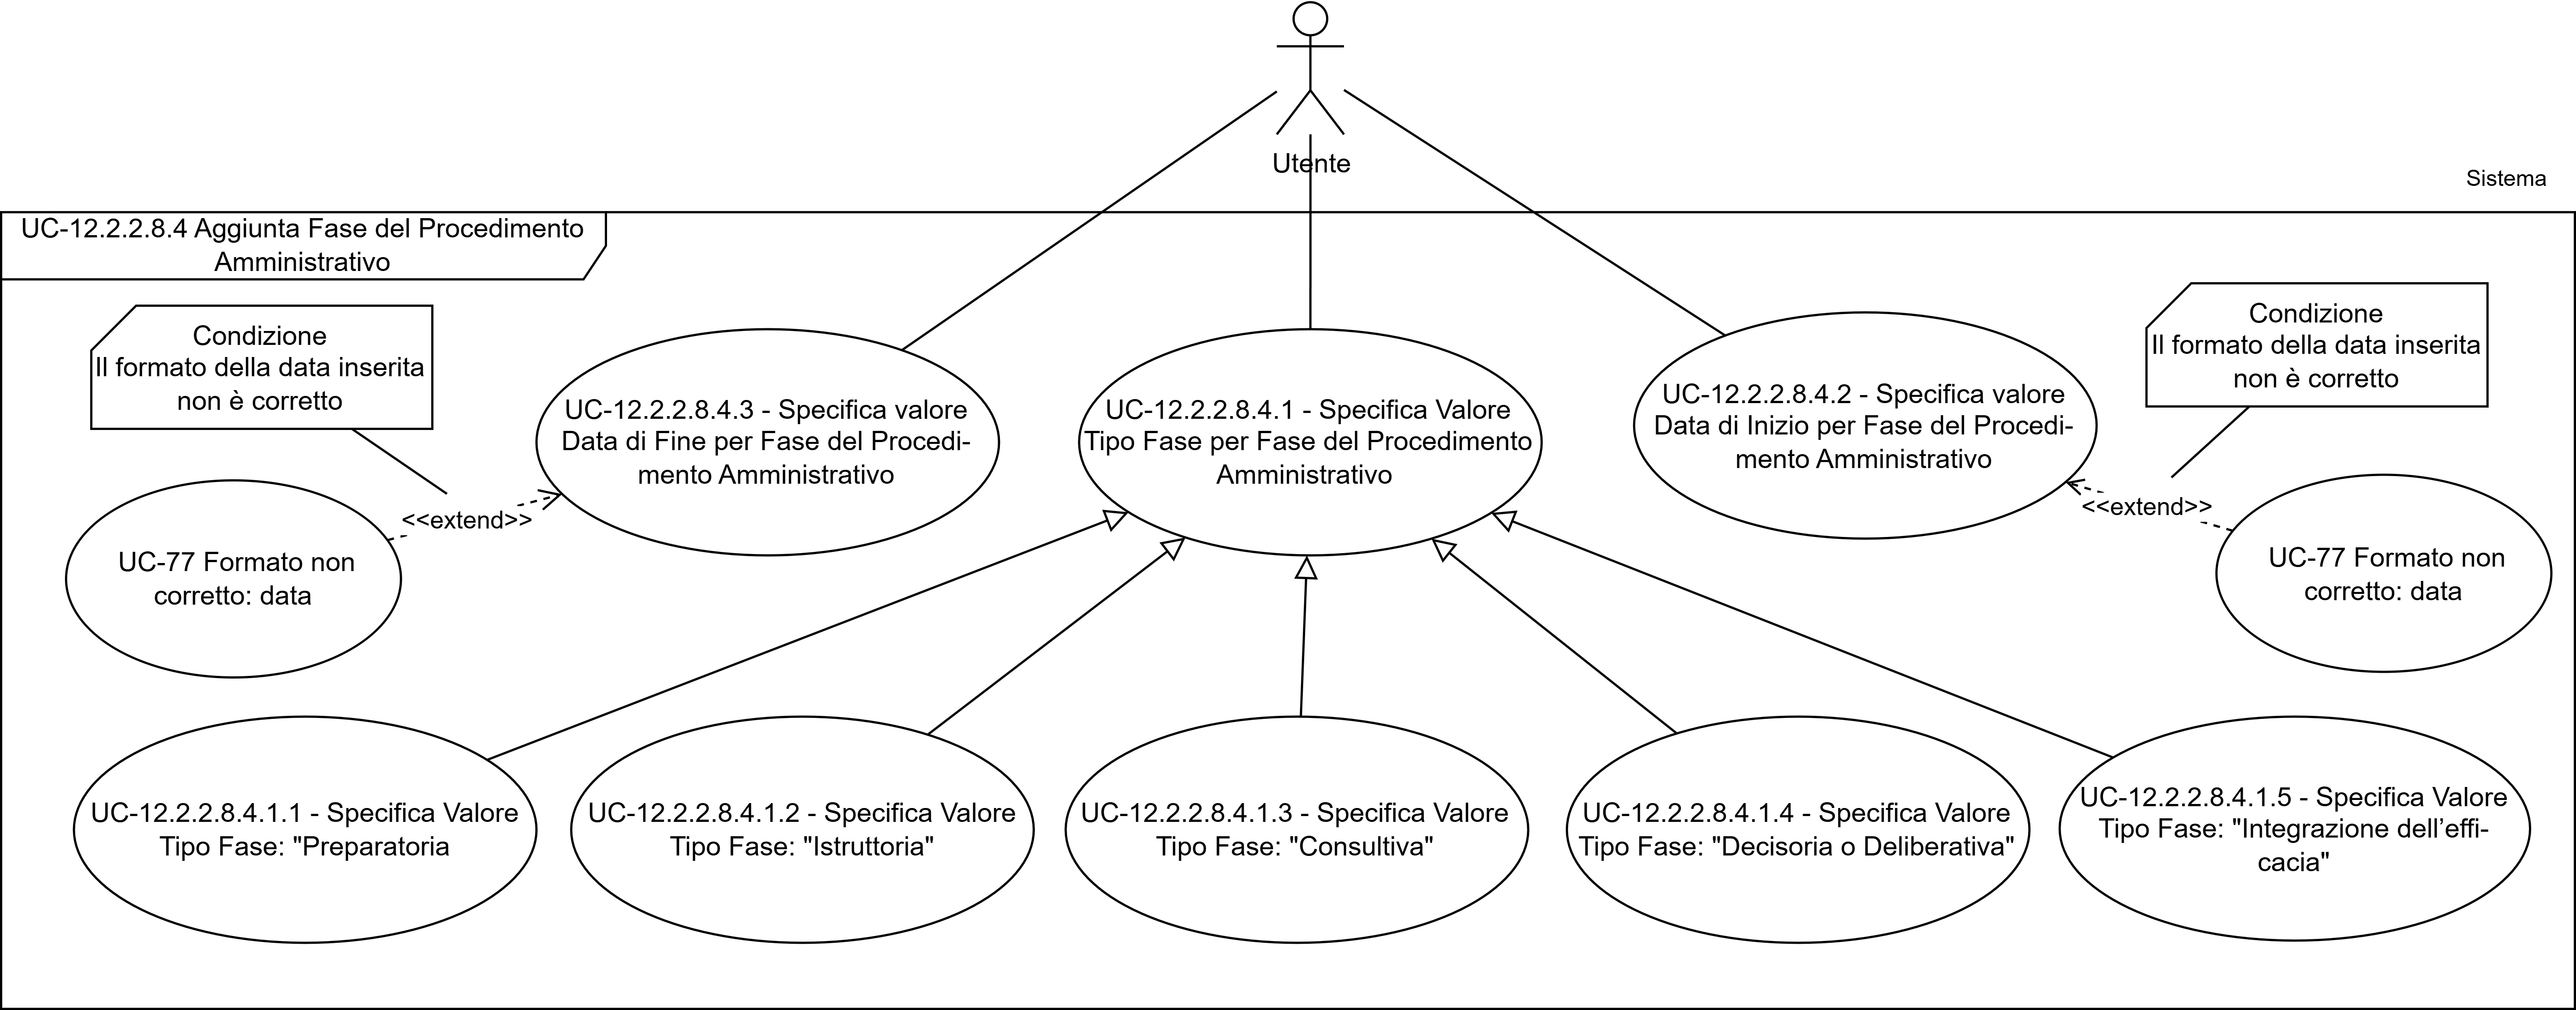
\includegraphics[width=1\textwidth]{../../assets/uml/UC12.2.2.8.4INC.png}
      \caption{Inclusioni \ref{addProcedimentoAmministrativo} - Specifica filtro Procedimento Amministrativo}
      \label{fig:addFasiProcedimentoAmministrativoInclusioni}
\end{figure}

\subsubdeepusecase{addValoreTipoFase}{Specifica Valore Tipo Fase per Fase del Procedimento Amministrativo}
\begin{itemize}
      \item \textbf{Attore Primario}: Utente
      \item \textbf{Precondizioni}: 
      \begin{itemize}
            \item L'Utente ha avviato l'applicazione
            \item L'Utente sta effettuando una ricerca nel DIP con filtri
            \item L'Utente ha specificato come tipo di documento: Aggregazione Documentale
            \item L'Utente sta specificando una Fase del Procedimento Amministrativo come parte del filtro Procedimento Amministrativo
      \end{itemize}
      \item \textbf{Postcondizioni}: Viene specificato il Tipo Fase per la Fase del Procedimento Amministrativo che si sta specificando.
      \item \textbf{Flusso Principale}:
      \begin{enumerate}
            \item L'Utente specifica il Tipo Fase per la Fase del Procedimento Amministrativo.
            \item Il sistema salva il valore del Tipo Fase per la fase che si sta specificando.
      \end{enumerate}
\end{itemize}

\abyssalusecase{addValoreTipoFasePreparatoria}{Specifica Valore Tipo Fase:  "Preparatoria"}
\begin{itemize}
      \item \textbf{Attore Primario}: Utente
      \item \textbf{Precondizioni}: 
      \begin{itemize}
            \item L'Utente ha avviato l'applicazione
            \item L'Utente sta effettuando una ricerca nel DIP con filtri
            \item L'Utente ha specificato come tipo di documento: Aggregazione Documentale
            \item L'Utente sta specificando una Fase del Procedimento Amministrativo come parte del filtro Procedimento Amministrativo
      \end{itemize}
      \item \textbf{Postcondizioni}: Viene selezionato "Preparatoria" come valore del Tipo Fase per la fase che si sta specificando.
      \item \textbf{Flusso Principale}:
      \begin{enumerate}
            \item L'Utente specifica il valore del Tipo Fase: "Preparatoria".
            \item Il sistema salva il valore del Tipo Fase per la fase che si sta specificando.
      \end{enumerate}
      \item \textbf{Specializza}: \ref{addValoreTipoFase}
\end{itemize}

\abyssalusecase{addValoreTipoFaseIstruttoria}{Specifica Valore Tipo Fase: "Istruttoria"}
\begin{itemize}
      \item \textbf{Attore Primario}: Utente
      \item \textbf{Precondizioni}: 
      \begin{itemize}
            \item L'Utente ha avviato l'applicazione
            \item L'Utente sta effettuando una ricerca nel DIP con filtri
            \item L'Utente ha specificato come tipo di documento: Aggregazione Documentale
            \item L'Utente sta specificando una Fase del Procedimento Amministrativo come parte del filtro Procedimento Amministrativo
      \end{itemize}
      \item \textbf{Postcondizioni}: Viene selezionato "Istruttoria" come valore del Tipo Fase per la fase che si sta specificando.
      \item \textbf{Flusso Principale}:
      \begin{enumerate}
            \item L'Utente specifica il valore del Tipo Fase: "Istruttoria".
            \item Il sistema salva il valore del Tipo Fase per la fase che si sta specificando.
      \end{enumerate}
      \item \textbf{Specializza}: \ref{addValoreTipoFase}
\end{itemize}

\abyssalusecase{addValoreTipoFaseConsultiva}{Specifica Valore Tipo Fase: "Consultiva"}
\begin{itemize}
      \item \textbf{Attore Primario}: Utente
      \item \textbf{Precondizioni}: 
      \begin{itemize}
            \item L'Utente ha avviato l'applicazione
            \item L'Utente sta effettuando una ricerca nel DIP con filtri
            \item L'Utente ha specificato come tipo di documento: Aggregazione Documentale
            \item L'Utente sta specificando una Fase del Procedimento Amministrativo come parte del filtro Procedimento Amministrativo
      \end{itemize}
      \item \textbf{Postcondizioni}: Viene selezionato "Consultiva" come valore del Tipo Fase per la fase che si sta specificando.
      \item \textbf{Flusso Principale}:
      \begin{enumerate}
            \item L'Utente specifica il valore del Tipo Fase: "Consultiva".
            \item Il sistema salva il valore del Tipo Fase per la fase che si sta specificando.
      \end{enumerate}
      \item \textbf{Specializza}: \ref{addValoreTipoFase}
\end{itemize}

\abyssalusecase{addValoreTipoFaseDecisoria}{Specifica Valore Tipo Fase: "Decisoria o Deliberativa"}
\begin{itemize}
      \item \textbf{Attore Primario}: Utente
      \item \textbf{Precondizioni}: 
      \begin{itemize}
            \item L'Utente ha avviato l'applicazione
            \item L'Utente sta effettuando una ricerca nel DIP con filtri
            \item L'Utente ha specificato come tipo di documento: Aggregazione Documentale
            \item L'Utente sta specificando una Fase del Procedimento Amministrativo come parte del filtro Procedimento Amministrativo
      \end{itemize}
      \item \textbf{Postcondizioni}: Viene selezionato "Decisoria o Deliberativa" come valore del Tipo Fase per la fase che si sta specificando.
      \item \textbf{Flusso Principale}:
      \begin{enumerate}
            \item L'Utente specifica il valore del Tipo Fase: "Decisoria o Deliberativa".
            \item Il sistema salva il valore del Tipo Fase per la fase che si sta specificando.
      \end{enumerate}
      \item \textbf{Specializza}: \ref{addValoreTipoFase}
\end{itemize}

\abyssalusecase{addValoreTipoFaseIntegrazione}{Specifica Valore Tipo Fase: "Integrazione dell'efficacia"}
\begin{itemize}
      \item \textbf{Attore Primario}: Utente
      \item \textbf{Precondizioni}: 
      \begin{itemize}
            \item L'Utente ha avviato l'applicazione
            \item L'Utente sta effettuando una ricerca nel DIP con filtri
            \item L'Utente ha specificato come tipo di documento: Aggregazione Documentale
            \item L'Utente sta specificando una Fase del Procedimento Amministrativo come parte del filtro Procedimento Amministrativo
      \end{itemize}
      \item \textbf{Postcondizioni}: Viene selezionato "Integrazione dell'efficacia" come valore del Tipo Fase per la fase che si sta specificando.
      \item \textbf{Flusso Principale}:
      \begin{enumerate}
            \item L'Utente specifica il valore del Tipo Fase: "Integrazione dell'efficacia".
            \item Il sistema salva il valore del Tipo Fase per la fase che si sta specificando.
      \end{enumerate}
      \item \textbf{Specializza}: \ref{addValoreTipoFase}
\end{itemize}

\subsubdeepusecase{addDataInizioFase}{Specifica valore Data di Inizio per Fase del Procedimento Amministrativo}
\begin{itemize}
      \item \textbf{Attore Primario}: Utente
      \item \textbf{Precondizioni}: 
      \begin{itemize}
            \item L'Utente ha avviato l'applicazione
            \item L'Utente sta effettuando una ricerca nel DIP con filtri
            \item L'Utente ha specificato come tipo di documento: Aggregazione Documentale
            \item L'Utente sta specificando una Fase del Procedimento Amministrativo come parte del filtro Procedimento Amministrativo
      \end{itemize}
      \item \textbf{Postcondizioni}: Viene specificata la Data di Inizio per la Fase del Procedimento Amministrativo che si sta specificando.
      \item \textbf{Flusso Principale}:
      \begin{enumerate}
            \item L'Utente specifica la Data di Inizio per la Fase del Procedimento Amministrativo.
            \item Il sistema salva il valore della Data di Inizio per la fase che si sta specificando.
      \end{enumerate}
      \item \textbf{Flusso Alternativo}:
      \begin{itemize}
            \item L'Utente inserisce una data non valida per il filtro Data di Inizio della Fase del Procedimento Amministrativo (formato data errato) (\ref{formatoNonCorrettoData})
      \end{itemize}
      \item \textbf{Estensioni}: \ref{formatoNonCorrettoData} Formato non corretto: data
\end{itemize}

\subsubdeepusecase{addDataFineFase}{Specifica valore Data di Fine per Fase del Procedimento Amministrativo}
\begin{itemize}
      \item \textbf{Attore Primario}: Utente
      \item \textbf{Precondizioni}: 
      \begin{itemize}
            \item L'Utente ha avviato l'applicazione
            \item L'Utente sta effettuando una ricerca nel DIP con filtri
            \item L'Utente ha specificato come tipo di documento: Aggregazione Documentale
            \item L'Utente sta specificando una Fase del Procedimento Amministrativo come parte del filtro Procedimento Amministrativo
      \end{itemize}
      \item \textbf{Postcondizioni}: Viene specificata la Data di Fine per la Fase del Procedimento Amministrativo che si sta specificando.
      \item \textbf{Flusso Principale}:
      \begin{enumerate}
            \item L'Utente specifica la Data di Fine per la Fase del Procedimento Amministrativo.
            \item Il sistema salva il valore della Data di Fine per la fase che si sta specificando.
      \end{enumerate}
      \item \textbf{Flusso Alternativo}:
      \begin{itemize}
            \item L'Utente inserisce una data non valida per il filtro Data di Fine della Fase del Procedimento Amministrativo (formato data errato) (\ref{formatoNonCorrettoData})
      \end{itemize}
      \item \textbf{Estensioni}: \ref{formatoNonCorrettoData} Formato non corretto: data
\end{itemize}

\deepusecase{addAssegnazione}{Specifica filtro Assegnazione}
\begin{itemize}
      \item \textbf{Attore Primario}: Utente
      \item \textbf{Precondizioni}: 
      \begin{itemize}
            \item L'Utente ha avviato l'applicazione
            \item L'Utente sta effettuando una ricerca nel DIP con filtri
            \item L'Utente ha specificato come tipo di documento: Aggregazione Documentale
            \item L'utente ha selezionato il filtro Assegnazione tra i campi specifici per tipo documentale
      \end{itemize}
      \item \textbf{Postcondizioni}: 
      \begin{itemize}
            \item L'Utente ha specificato i valori del filtro Assegnazione
            \item Il filtro Assegnazione è parametro per la ricerca con filtri e per la generazione del risultato
      \end{itemize}
      \item \textbf{Flusso Principale}:
      \begin{enumerate}
            \item L'Utente aggiunge uno o più valori per "Assegnazione". (\ref{addValoreAssegnazione})(0...n).
            \item Il sistema imposta i valori del filtro come parametri per la ricerca.
      \end{enumerate}
      \item \textbf{Inclusioni}: \ref{addValoreAssegnazione} Aggiunta Valore Assegnazione
\end{itemize}
\begin{figure}[H]
      \centering
      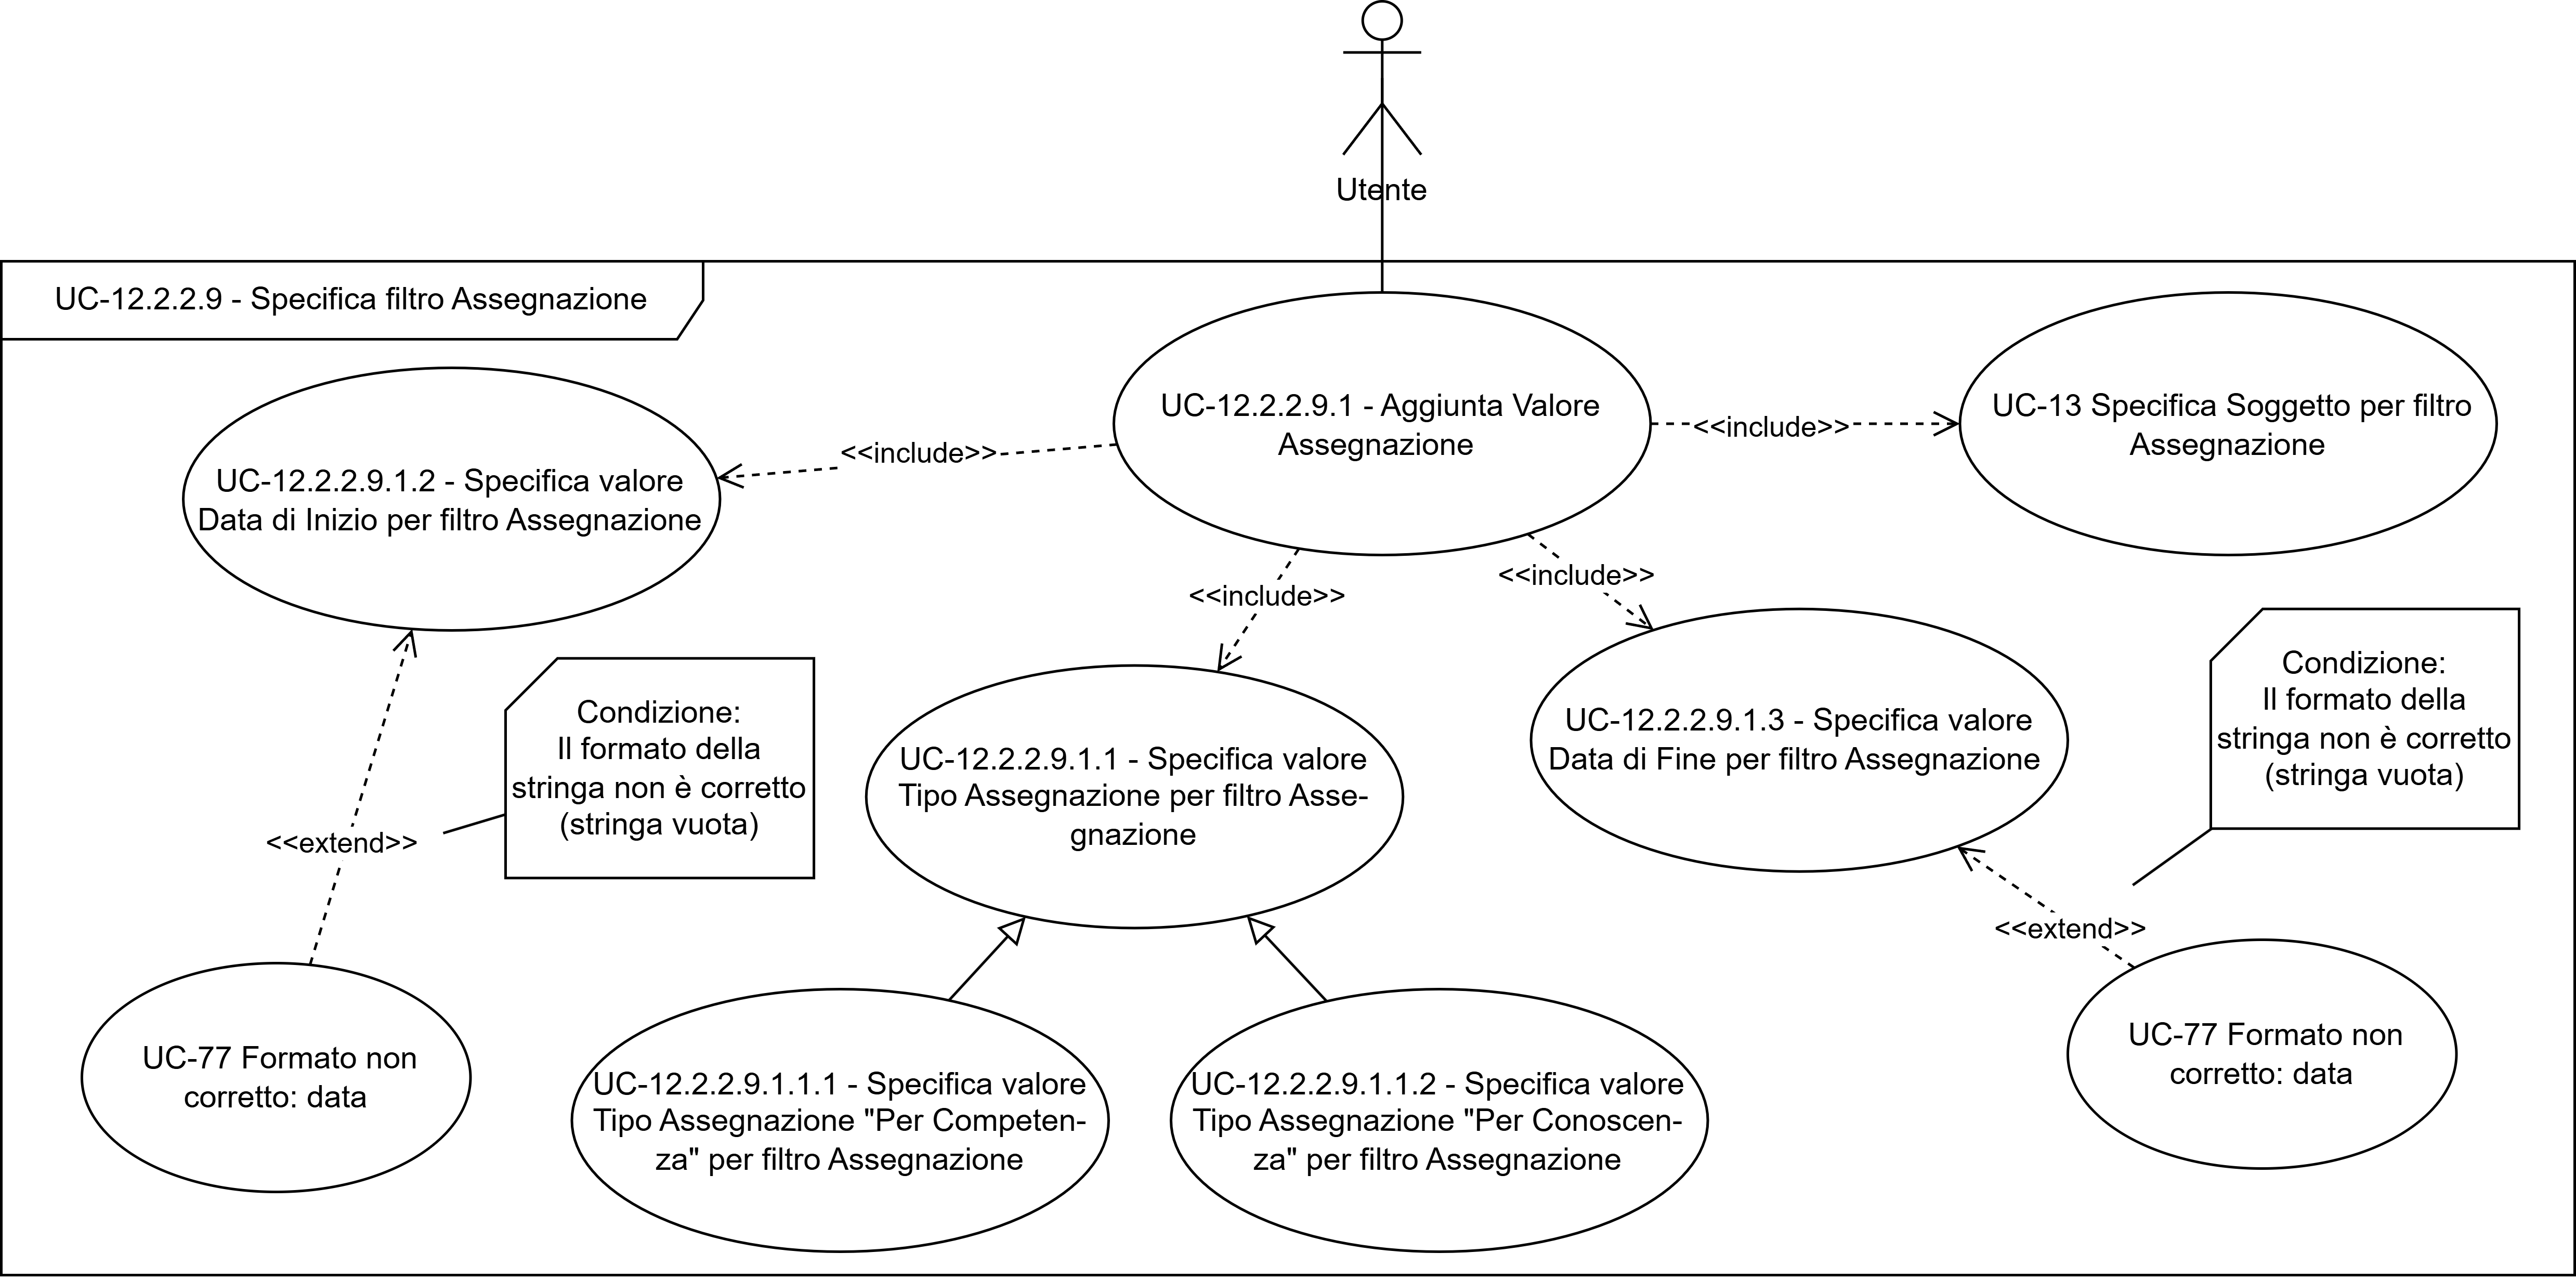
\includegraphics[width=1\textwidth]{../../assets/uml/UC12.2.2.9INC.png}
      \caption{Inclusioni \ref{addAssegnazione} - Specifica filtro Assegnazione}
      \label{fig:inclusioniSpecificaFiltriAssegnazione}
\end{figure}
      
\subdeepusecase{addValoreAssegnazione}{Aggiunta Valore Assegnazione}
\begin{itemize}
      \item \textbf{Attore Primario}: Utente
      \item \textbf{Precondizioni}: 
      \begin{itemize}
            \item L'Utente ha avviato l'applicazione
            \item L'Utente sta effettuando una ricerca nel DIP con filtri
            \item L'Utente ha specificato come tipo di documento: Aggregazione Documentale
            \item L'Utente sta specificando un filtro che richiede un valore di Assegnazione
      \end{itemize}
      \item \textbf{Postcondizioni}: Viene specificato un valore di Assegnazione e aggiunto al filtro che l'Utente sta specificando.
      \item \textbf{Flusso Principale}:
      \begin{enumerate}
            \item L'utente specifica:
            \begin{itemize}
                  \item Tipo Assegnazione.
                  \item Soggetto Assegnatario. (\ref{addSoggetto})
                  \item Data di Inizio.
                  \item Data di Fine.
            \end{itemize}
            \item Il sistema salva il valore di assegnazione come parte del filtro Assegnazione.
      \end{enumerate}
      \item \textbf{Inclusioni}: \begin{itemize}
            \item \ref{addValoreTipoAssegnazione} Specifica valore Tipo Assegnazione per filtro Assegnazione
            \item \ref{addSoggetto} Specifica Soggetto per filtro Assegnazione
            \item \ref{addValoreDataInizioAssegnazione} Specifica Data di Inizio per filtro Assegnazione
            \item \ref{addValoreDataFineAssegnazione} Specifica Data di Fine per filtro Assegnazione
      \end{itemize}
\end{itemize}

\subsubdeepusecase{addValoreTipoAssegnazione}{Specifica valore Tipo Assegnazione per filtro Assegnazione}
\begin{itemize}
      \item \textbf{Attore Primario}: Utente
      \item \textbf{Precondizioni}: 
      \begin{itemize}
            \item L'Utente ha avviato l'applicazione
            \item L'Utente sta effettuando una ricerca nel DIP con filtri
            \item L'Utente ha specificato come tipo di documento: Aggregazione Documentale
            \item L'Utente sta specificando un valore di Assegnazione come parte dei filtri per la ricerca
      \end{itemize}
      \item \textbf{Postcondizioni}: Viene specificato un valore per il Tipo Assegnazione per l'assegnazione che si sta specificando.
      \item \textbf{Flusso Principale}:
      \begin{enumerate}
            \item L'Utente specifica il valore del Tipo Assegnazione per il filtro Assegnazione.
            \item Il sistema salva il valore del Tipo Assegnazione per l'assegnazione che si sta specificando.
      \end{enumerate}
\end{itemize}

\abyssalusecase{addValoreTipoAssegnazionePerCompetenza}{Specifica valore Tipo Assegnazione "Per Competenza" per filtro Assegnazione}
\begin{itemize}
      \item \textbf{Attore Primario}: Utente
      \item \textbf{Precondizioni}: 
      \begin{itemize}
            \item L'Utente ha avviato l'applicazione
            \item L'Utente sta effettuando una ricerca nel DIP con filtri
            \item L'Utente ha specificato come tipo di documento: Aggregazione Documentale
            \item L'Utente sta specificando un valore di Assegnazione come parte dei filtri per la ricerca
      \end{itemize}
      \item \textbf{Postcondizioni}: Viene selezionato "Per Competenza" come valore del Tipo Assegnazione per l'assegnazione che si sta specificando.
      \item \textbf{Flusso Principale}:
      \begin{enumerate}
            \item L'Utente specifica il valore del Tipo Assegnazione: "Per Competenza".
            \item Il sistema salva il valore del Tipo Assegnazione per l'assegnazione che si sta specificando.
      \end{enumerate}
      \item \textbf{Specializza}: \ref{compilaValoreFiltroAssegnazione} Compila valore filtro tipo assegnazione
\end{itemize}

\abyssalusecase{addValoreTipoAssegnazionePerConoscenza}{Specifica valore Tipo Assegnazione "Per Conoscenza" per filtro Assegnazione}
\begin{itemize}
      \item \textbf{Attore Primario}: Utente
      \item \textbf{Precondizioni}: 
      \begin{itemize}
            \item L'Utente ha avviato l'applicazione
            \item L'Utente sta effettuando una ricerca nel DIP con filtri
            \item L'Utente ha specificato come tipo di documento: Aggregazione Documentale
            \item L'Utente sta specificando un valore di Assegnazione come parte dei filtri per la ricerca
      \end{itemize}
      \item \textbf{Postcondizioni}: Viene selezionato "Per Conoscenza" come valore del Tipo Assegnazione per l'assegnazione che si sta specificando.
      \item \textbf{Flusso Principale}:
      \begin{enumerate}
            \item L'Utente specifica il valore del Tipo Assegnazione: "Per Conoscenza".
            \item Il sistema salva il valore del Tipo Assegnazione per l'assegnazione che si sta specificando.
      \end{enumerate}
      \item \textbf{Specializza}: \ref{compilaValoreFiltroAssegnazione} Compila valore filtro tipo assegnazione
\end{itemize}

\subsubdeepusecase{addValoreDataInizioAssegnazione}{Specifica valore Data di Inizio per filtro Assegnazione}
\begin{itemize}
      \item \textbf{Attore Primario}: Utente
      \item \textbf{Precondizioni}: 
      \begin{itemize}
            \item L'Utente ha avviato l'applicazione
            \item L'Utente sta effettuando una ricerca nel DIP con filtri
            \item L'Utente ha specificato come tipo di documento: Aggregazione Documentale
            \item L'Utente sta specificando un valore di Assegnazione come parte dei filtri per la ricerca
      \end{itemize}
      \item \textbf{Postcondizioni}: Viene specificata la Data di Inizio per il valore di Assegnazione e salvata per l'assegnazione che si sta specificando.
      \item \textbf{Flusso Principale}:
      \begin{enumerate}
            \item L'Utente specifica la Data di Inizio per il valore di Assegnazione.
            \item Il sistema salva il valore della Data di Inizio per l'assegnazione che si sta specificando.
      \end{enumerate}
      \item \textbf{Flusso Alternativo}:
      \begin{itemize}
            \item L'Utente inserisce una data non valida per il filtro Data di Inizio dell'Assegnazione (formato data errato) (\ref{formatoNonCorrettoData})
      \end{itemize}
      \item \textbf{Estensioni}: \ref{formatoNonCorrettoData} Formato non corretto: data
\end{itemize}

\subsubdeepusecase{addValoreDataFineAssegnazione}{Specifica valore Data di Fine per filtro Assegnazione}
\begin{itemize}
      \item \textbf{Attore Primario}: Utente
      \item \textbf{Precondizioni}: 
      \begin{itemize}
            \item L'Utente ha avviato l'applicazione
            \item L'Utente sta effettuando una ricerca nel DIP con filtri
            \item L'Utente ha specificato come tipo di documento: Aggregazione Documentale
            \item L'Utente sta specificando un valore di Assegnazione come parte dei filtri per la ricerca
      \end{itemize}
      \item \textbf{Postcondizioni}: Viene specificata la Data di Fine per il valore di Assegnazione e salvata per l'assegnazione che si sta specificando.
      \item \textbf{Flusso Principale}:
      \begin{enumerate}
            \item L'Utente specifica la Data di Fine per il valore di Assegnazione.
            \item Il sistema salva il valore della Data di Fine per l'assegnazione che si sta specificando.
      \end{enumerate}
      \item \textbf{Flusso Alternativo}:
      \begin{itemize}
            \item L'Utente inserisce una data non valida per il filtro Data di Fine dell'Assegnazione (formato data errato) (\ref{formatoNonCorrettoData})
      \end{itemize}
      \item \textbf{Estensioni}: \ref{formatoNonCorrettoData} Formato non corretto: data
\end{itemize}
      
\deepusecase{addProgressivoAggregazione}{Specifica filtro Progressivo Aggregazione}
\begin{itemize}
      \item \textbf{Attore Primario}: Utente
      \item \textbf{Precondizioni}: 
      \begin{itemize}
            \item L'Utente ha avviato l'applicazione
            \item L'Utente sta effettuando una ricerca nel DIP con filtri
            \item L'Utente ha specificato come tipo di documento: Aggregazione Documentale
            \item L'utente ha selezionato il filtro Progressivo dell'Aggregazione tra i campi specifici per tipo documentale
      \end{itemize}
      \item \textbf{Postcondizioni}: 
      \begin{itemize}
            \item L'Utente ha specificato i valori del filtro Progressivo dell'Aggregazione (\ref{compilaValoreFiltroNumero})
            \item Il filtro Progressivo dell'Aggregazione è parametro per la ricerca con filtri e per la generazione del risultato
      \end{itemize}
      \item \textbf{Flusso Principale}:
      \begin{enumerate}
            \item L'Utente specifica il numero Progressivo dell'Aggregazione.
            \item Il sistema imposta questo valore come parametro per la ricerca.
      \end{enumerate}
      \item \textbf{Flusso Alternativo}:
      \begin{enumerate}
            \item L'Utente inserisce un valore non valido per il filtro Progressivo dell'Aggregazione (formato numero errato) (\ref{formatoNonCorrettoNumero})
      \end{enumerate}
      \item \textbf{Estensioni}: \ref{formatoNonCorrettoNumero} Formato non corretto: numero
\end{itemize}


\subusecase{addCustomMetadata}{Specifica filtri per Custom Metadata}
\begin{itemize}
      \item \textbf{Attore Primario}: Utente
      \item \textbf{Precondizioni}: \begin{itemize}
            \item L'Utente ha avviato l'applicazione
            \item L'Utente sta effettuando una ricerca nel DIP con filtri
      \end{itemize}
      \item \textbf{Postcondizioni}: Vengono specificati i filtri per i custom metadata e utilizzati per la generazione del risultato.
      \item \textbf{Flusso Principale}:
      \begin{enumerate}
            \item L'Utente, specifica uno o più filtri per i metadati custom (\ref{addFiltroMetadatoCustom}).
      \end{enumerate}
      \item \textbf{Inclusioni}: \ref{addFiltroMetadatoCustom} Specifica filtro Metadato Custom
      \item \textbf{Nota}: Per costruzione aziendale i custom metadata sono tutti stringhe e quindi l'inserimento e la validazione seguono le regole dei campi di testo liberi.
\end{itemize}
\begin{figure}[H]
      \centering
      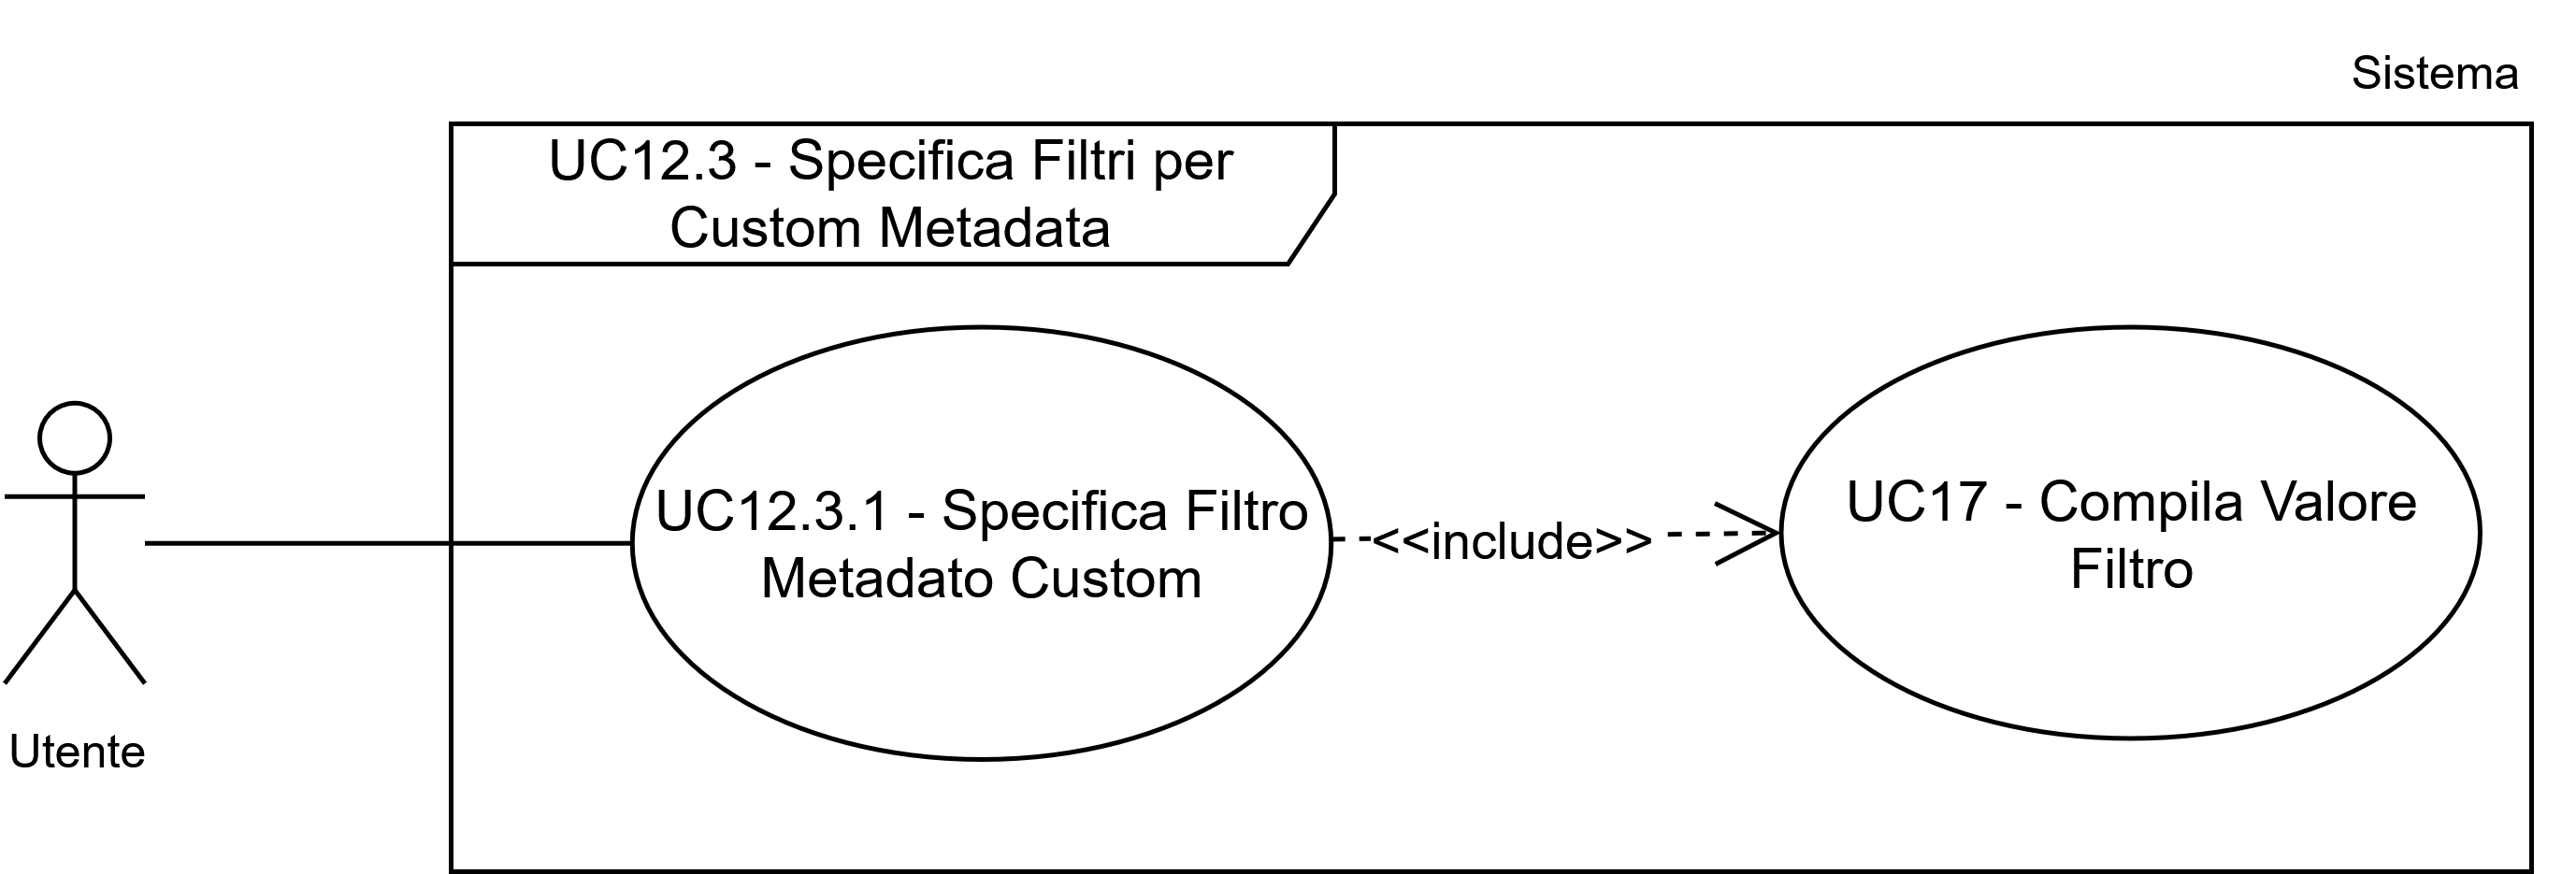
\includegraphics[width=0.9\textwidth]{../../assets/uml/UC12.3INC.png}
      \caption{Inclusioni \ref{addCustomMetadata} - Specifica filtri per Custom Metadata}
      \label{fig:inclusioniSpecificaFiltriCustomMetadata}
\end{figure}

\subsubusecase{addFiltroMetadatoCustom}{Specifica filtro Metadato Custom}
\begin{itemize}
      \item \textbf{Attore Primario}: Utente
      \item \textbf{Precondizioni}: \begin{itemize}
            \item L'Utente ha avviato l'applicazione
            \item L'Utente sta effettuando una ricerca nel DIP con filtri
            \end{itemize}
      \item \textbf{Postcondizioni}: Il filtro aggiunto dall'Utente è parametro per la ricerca con filtri e per la generazione del risultato.
      \item \textbf{Flusso Principale}:
      \begin{enumerate}
            \item L'Utente specifica il nome del metadato custom. (\ref{compilaValoreFiltroStringa}).
            \item L'Utente specifica il valore del metadato custom per cui ricercare. (\ref{compilaValoreFiltroStringa}).
            \item Il sistema imposta questi valori come parametro per la ricerca.
      \end{enumerate}
      \item \textbf{Flusso Alternativo}:
      \begin{itemize}
            \item L'Utente inserisce un valore non valido per il filtro del metadato custom (stringa vuota) (\ref{formatoNonCorrettoStringa})
      \end{itemize}
      \item \textbf{Inclusioni}: \ref{compilaValoreFiltroStringa} Compila valore filtro stringa
      \item \textbf{Estensioni}: \ref{formatoNonCorrettoStringa} Formato non corretto: stringa
\end{itemize}

\usecase{addSoggetto}{Aggiunta Soggetto ad un filtro}
\begin{itemize}
      \item \textbf{Attore Primario}: Utente
      \item \textbf{Precondizioni}: 
      \begin{itemize}
            \item L'Utente ha avviato l'applicazione
            \item L'Utente sta effettuando una ricerca nel DIP con filtri
            \item L'Utente sta specificando un filtro che prevede l'aggiunta di soggetti
      \end{itemize}
      \item \textbf{Postcondizioni}: Viene specificato un soggetto e aggiunto al filtro che l'Utente sta specificando.
      \item \textbf{Flusso Principale}:
      \begin{enumerate}
            \item L'utente specifica il ruolo del soggetto tra quelli disponibili per il tipo di documento scelto. (\ref{specificaRuoloSoggetto}).
            \item L'utente specifica il tipo di soggetto tra quelli disponibili per il ruolo selezionato. (\ref{specificaTipoSoggetto}).
            \item L'utente specifica i valori dei campi per cui ricercare, relativi al tipo di soggetto selezionato (\ref{addDettagliSoggetto}).
            \item Viene aggiunto un soggetto con le specifiche indicate al filtro che l'Utente sta specificando.
      \end{enumerate}
      \item \textbf{Inclusioni}: 
      \begin{itemize}
            \item \ref{specificaRuoloSoggetto} Specifica ruolo del soggetto
            \item \ref{specificaTipoSoggetto} Specifica tipo di soggetto
            \item \ref{addDettagliSoggetto} Specifica dettagli soggetto
      \end{itemize}
\end{itemize}
\begin{figure}[H]
      \centering
      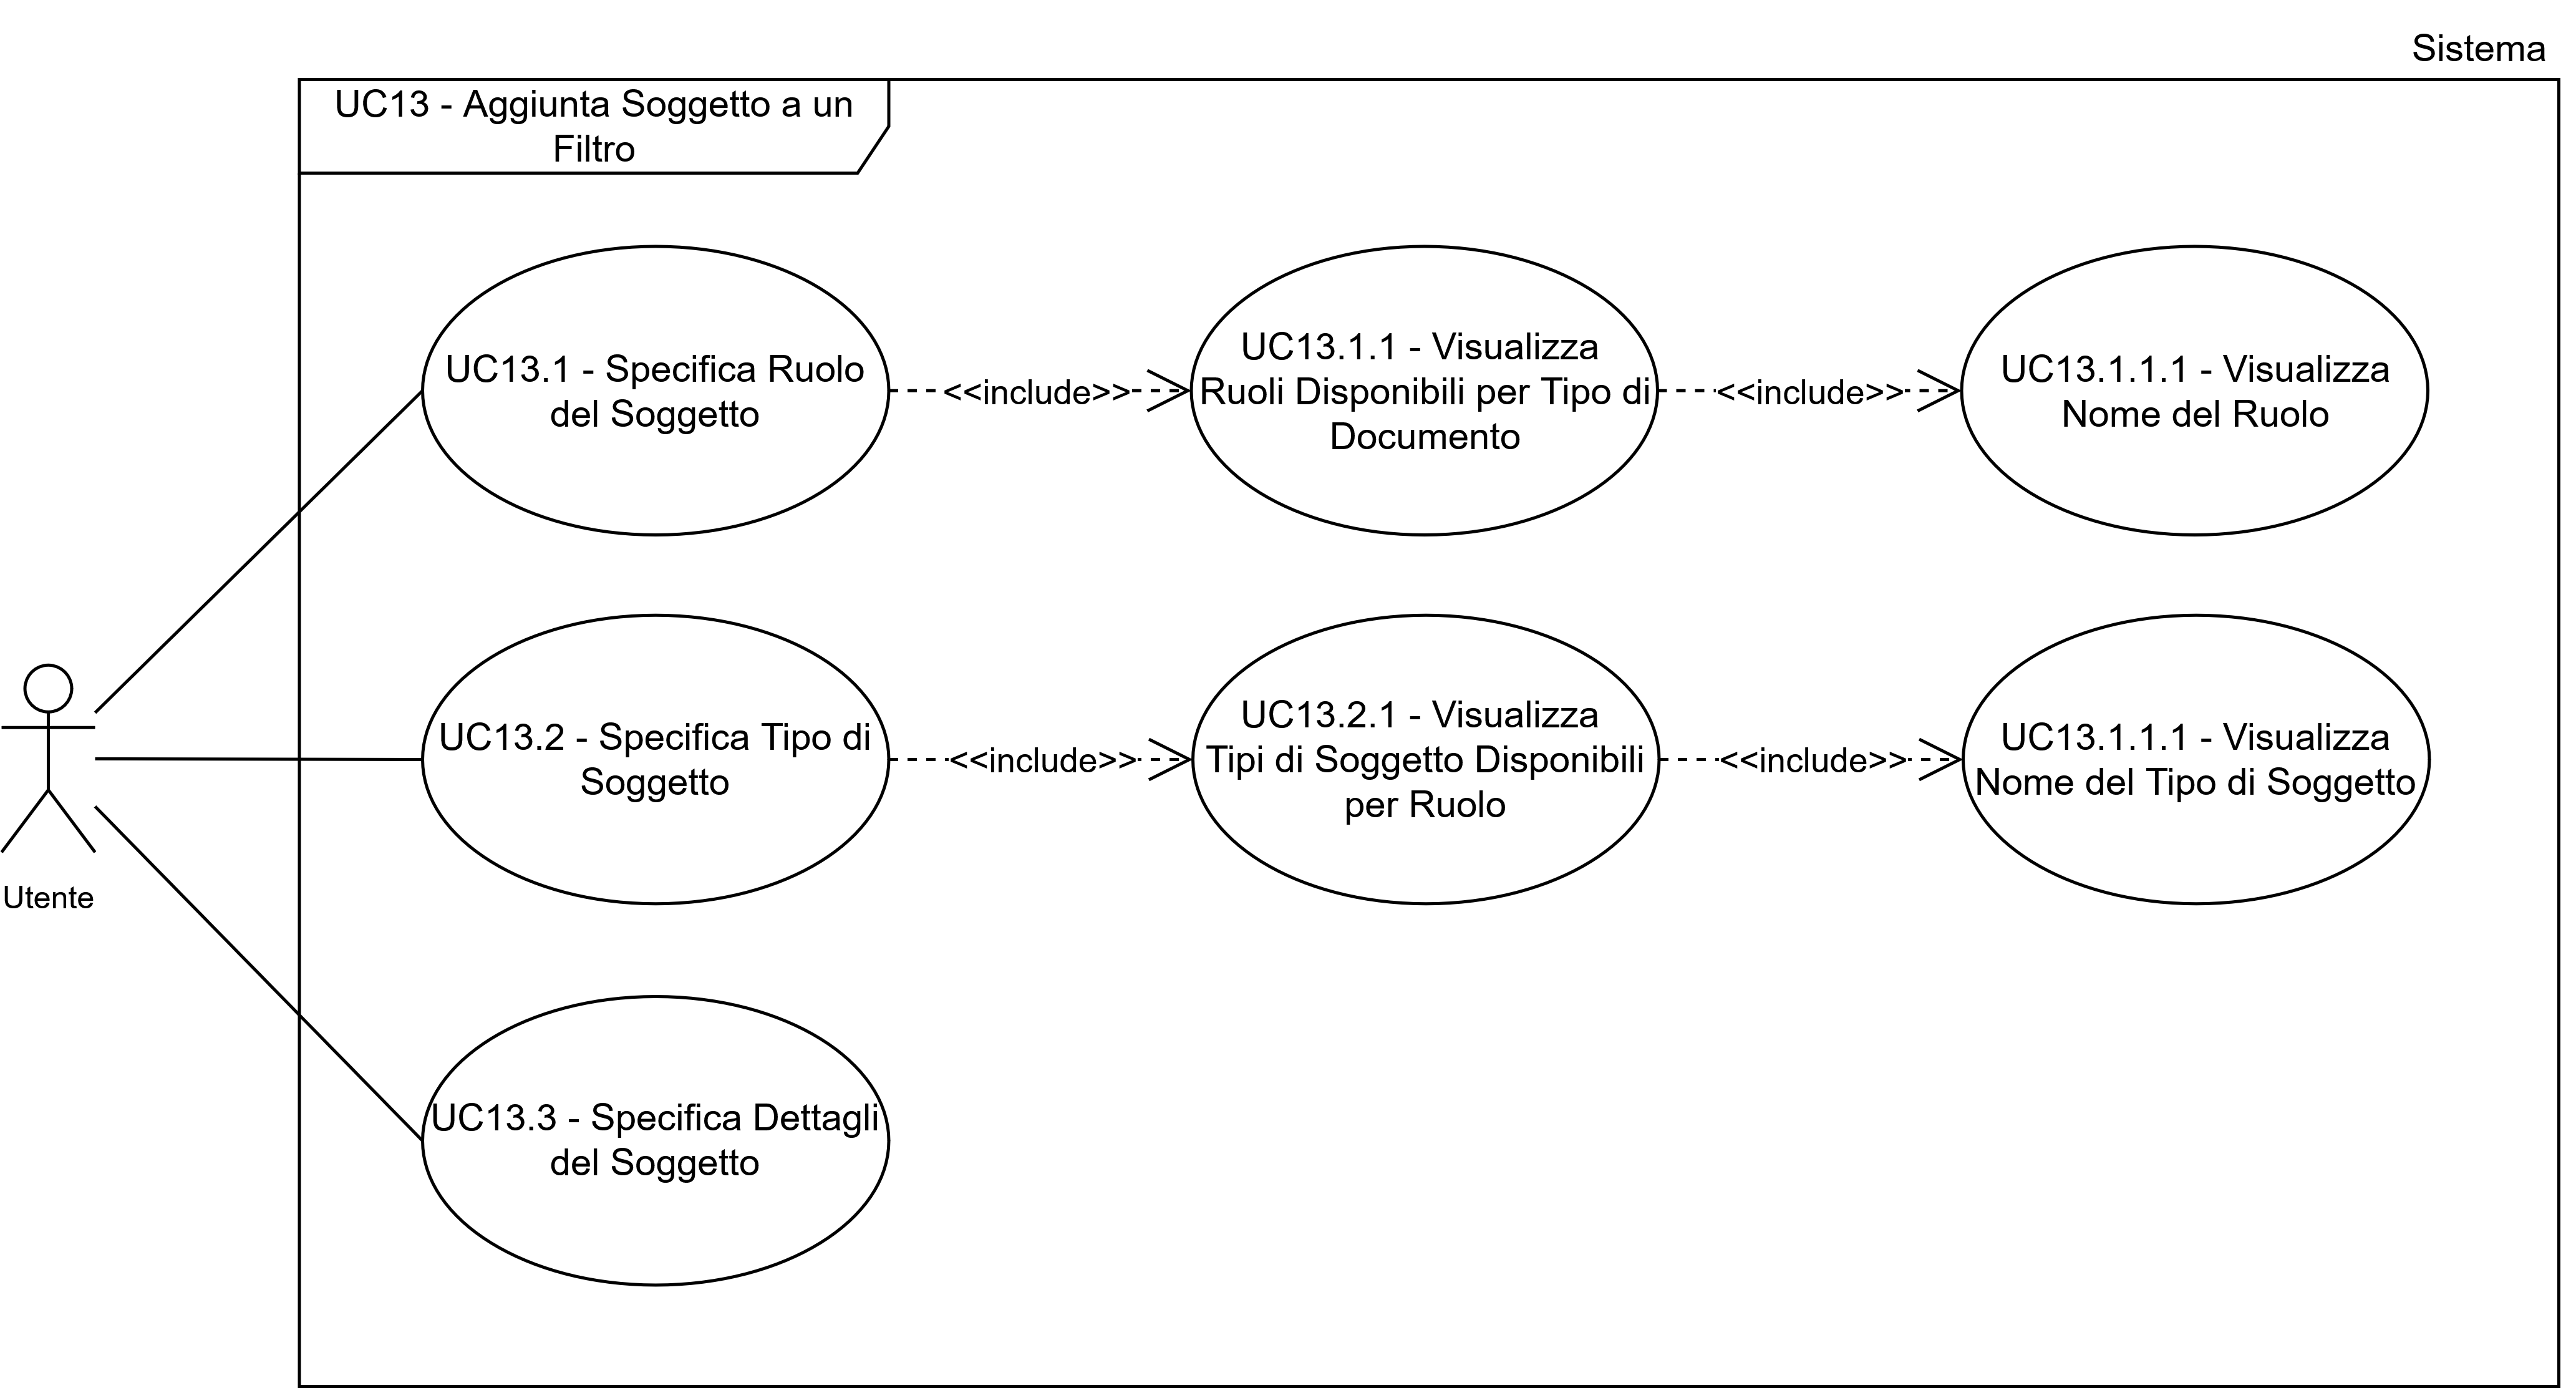
\includegraphics[width=0.4\textwidth]{../../assets/uml/UC13INC.png}
      \caption{Inclusioni \ref{addSoggetto} - Aggiunta Soggetto ad un filtro}
      \label{fig:inclusioniAggiuntaSoggetto}
\end{figure}

\subusecase{specificaRuoloSoggetto}{Specifica ruolo del soggetto}
\begin{itemize}
      \item \textbf{Attore Primario}: Utente
      \item \textbf{Precondizioni}: 
      \begin{itemize}
            \item L'Utente ha avviato l'applicazione
            \item L'Utente sta effettuando una ricerca nel DIP con filtri
            \item L'Utente ha specificato il filtro Tipo di Documento
            \item L'Utente sta aggiungendo un soggetto ad un filtro
      \end{itemize}
      \item \textbf{Postcondizioni}: Viene specificato il ruolo del soggetto che l'utente sta aggiungendo, in base alla specifica del filtro Tipo di Documento.
      \item \textbf{Flusso Principale}:
            \begin{enumerate}
                  \item L'Utente seleziona il Ruolo tra quelli disponibili per il tipo di documento selezionato.
                  \item Il sistema salva il ruolo selezionato per il soggetto che l'Utente sta aggiungendo.
            \end{enumerate}
\end{itemize}

\subusecase{specificaTipoSoggetto}{Specifica tipo di soggetto}
\begin{itemize}
      \item \textbf{Attore Primario}: Utente
      \item \textbf{Precondizioni}: 
      \begin{itemize}
            \item L'Utente ha avviato l'applicazione
            \item L'Utente sta effettuando una ricerca nel DIP con filtri
            \item L'Utente sta aggiungendo un soggetto ad un filtro
            \item L'Utente ha specificato il ruolo del soggetto
      \end{itemize}
      \item \textbf{Postcondizioni}: Viene specificato il tipo del soggetto che l'utente sta aggiungendo, in base al ruolo selezionato per il soggetto che l'Utente sta aggiungendo.
      \item \textbf{Flusso Principale}:
            \begin{enumerate}
                  \item L'Utente seleziona il Tipo di Soggetto tra quelli disponibili per il ruolo selezionato (per il soggetto che l'Utente sta aggiungendo).
                  \item Il sistema salva il tipo di soggetto selezionato per il soggetto che l'Utente sta aggiungendo.
            \end{enumerate}
\end{itemize}

\subusecase{addDettagliSoggetto}{Specifica dettagli soggetto}
\begin{figure}[H]
      \centering
      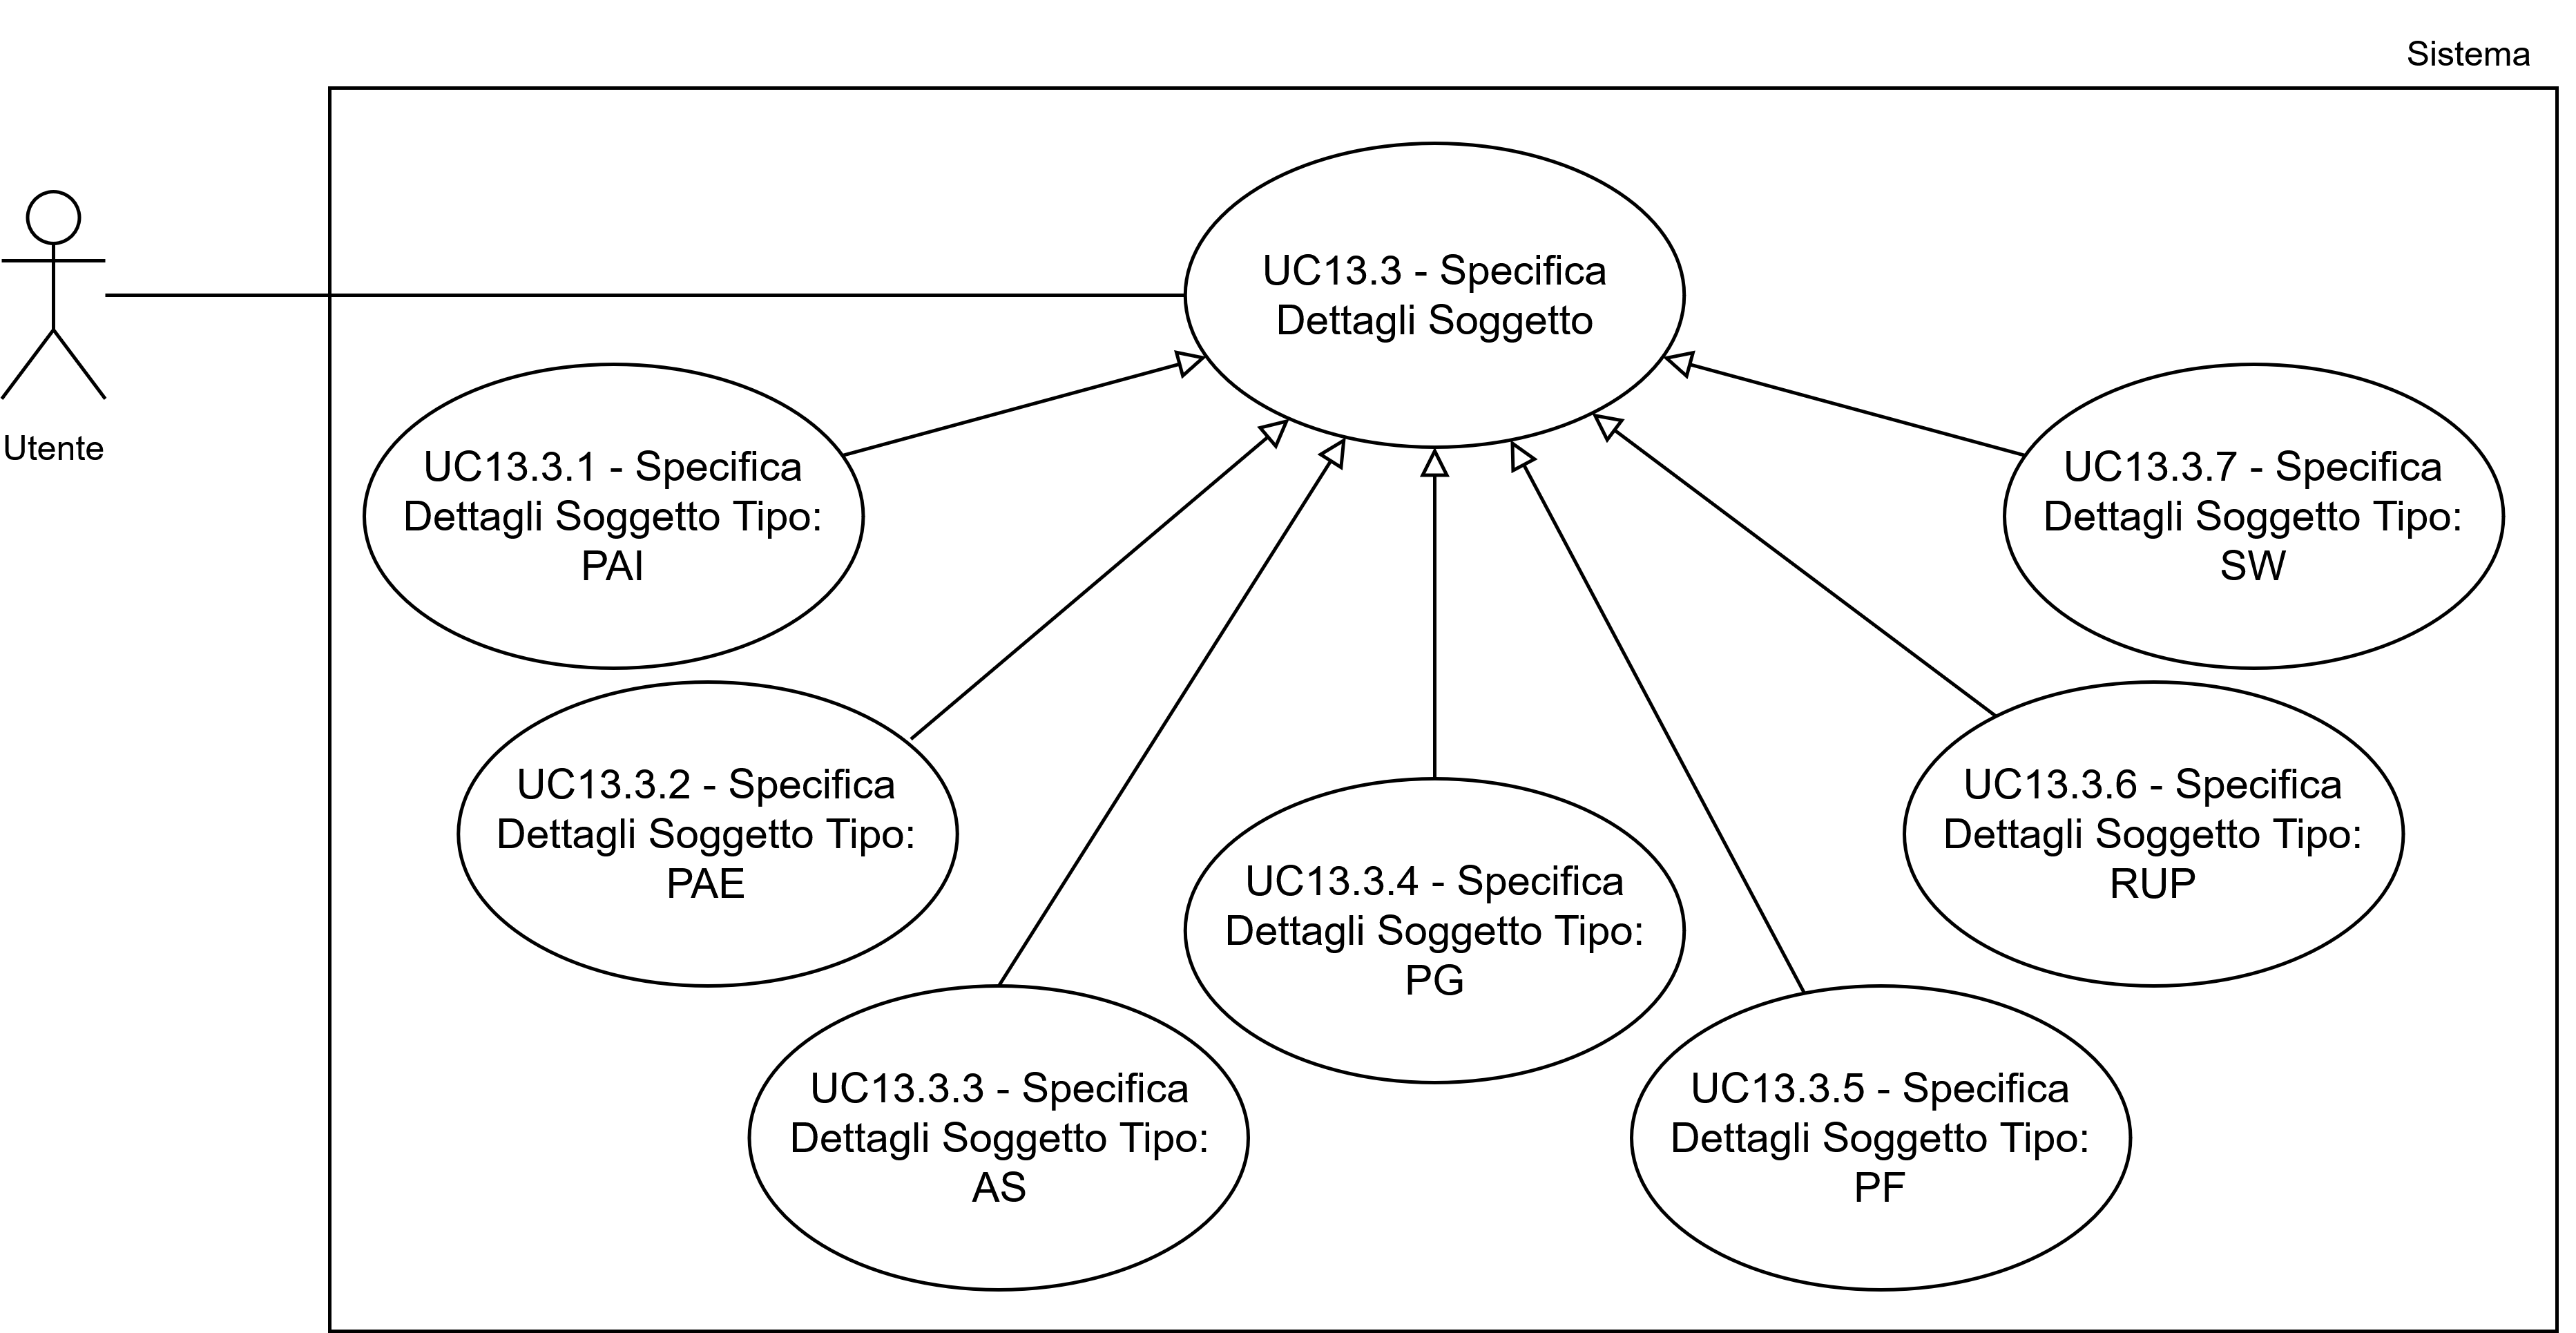
\includegraphics[width=1\textwidth]{../../assets/uml/UC13.3.png}
      \caption{\ref{addDettagliSoggetto} - Specifica dettagli soggetto}
      \label{fig:uc_addDettagliSoggetto}
\end{figure}
\begin{itemize}
      \item \textbf{Attore Primario}: Utente
      \item \textbf{Precondizioni}: 
      \begin{itemize}
            \item L'Utente ha avviato l'applicazione
            \item L'Utente sta effettuando una ricerca nel DIP con filtri
            \item L'Utente sta aggiungendo un soggetto, di cui ha specificato il tipo, ad un filtro. (\ref{specificaTipoSoggetto})
      \end{itemize}
      \item \textbf{Postcondizioni}: Le specifiche aggiunte dall'Utente sono salvate per il soggetto che sta aggiungendo.
      \item \textbf{Flusso Principale}:
      \begin{enumerate}
            \item L'Utente inserisce i dettagli del tipo di soggetto specificato. (da \ref{addDettagliPAI} a \ref{addDettagliSW})
            \item Il sistema salva i dettagli inseriti per il soggetto che l'utente sta aggiungendo.
      \end{enumerate}
\end{itemize}

\subsubusecase{addDettagliPAI}{Specifica dettagli soggetto tipo: PAI}
\begin{itemize}
      \item \textbf{Attore Primario}: Utente
      \item \textbf{Precondizioni}: 
      \begin{itemize}
            \item L'Utente ha avviato l'applicazione
            \item L'Utente sta effettuando una ricerca nel DIP con filtri
            \item L'Utente sta aggiungendo un soggetto di tipo: \glossario{PAI} ad un filtro.
      \end{itemize}
      \item \textbf{Postcondizioni}:  Le specifiche aggiunte dall'Utente sono salvate per il soggetto che sta aggiungendo.
      \item \textbf{Flusso Principale}:
            \begin{enumerate}
                  \item L'Utente inserisce i valori per i campi:
                        \begin{itemize}
                              \item Denominazione Amministrazione/ Codice \glossario{IPA}
                              \item Denominazione Amministrazione \glossario{AOO}/ Codice IPA AOO
                              \item Denominazione Amministrazione \glossario{UOR}/ Codice IPA UOR
                              \item Indirizzi Digitali di Riferimento
                        \end{itemize}
                  \item Il sistema salva i dettagli inseriti per il soggetto che l'utente sta aggiungendo.
            \end{enumerate}
      \item \textbf{Inclusioni}: \begin{itemize}
            \item \ref{addValoreDenominazioneAmmIPA}
            \item \ref{addValoreDenominazioneAmmAOO}
            \item \ref{addValoreDenominazioneAmmUOR}
            \item \ref{addValoreIndirizziDigitali}
      \end{itemize}
      \item \textbf{Specializza}: \ref{addDettagliSoggetto} Specifica dettagli soggetto
\end{itemize}

\deepusecase{addValoreDenominazioneAmmIPA}{Specifica valore Denominazione Amministrazione/ Codice IPA} \label{addValoreDenominazioneAmmIPA}
\begin{itemize}
      \item \textbf{Attore Primario}: Utente
      \item \textbf{Precondizioni}: 
      \begin{itemize}            
            \item L'Utente ha avviato l'applicazione
            \item L'Utente sta effettuando una ricerca nel DIP con filtri
            \item L'Utente sta specificando i dettagli di un soggetto di tipo PAI o AS
      \end{itemize}
      \item \textbf{Postcondizioni}: Viene specificato un valore per il campo Denominazione Amministrazione/ Codice IPA e associato al soggetto che l'Utente sta aggiungendo.
      \item \textbf{Flusso Principale}:
            \begin{enumerate}
                  \item L'Utente inserisce il valore per il campo Denominazione Amministrazione/ Codice IPA.
                  \item Il sistema salva il valore inserito per il campo Denominazione Amministrazione/ Codice IPA e lo associa al soggetto che l'Utente sta aggiungendo.
            \end{enumerate}
      \item \textbf{Flusso Alternativo}:
            \begin{itemize}
                  \item L'Utente inserisce un valore non valido per il campo Denominazione Amministrazione/ Codice IPA (stringa vuota) (\ref{formatoNonCorrettoStringa})
            \end{itemize}
      \item \textbf{Estensioni}: \ref{formatoNonCorrettoStringa} Formato non corretto: stringa
\end{itemize}

\deepusecase{addValoreDenominazioneAmmAOO}{Specifica valore Denominazione Amministrazione AOO/ Codice IPA AOO} \label{addValoreDenominazioneAmmAOO}
\begin{itemize}
      \item \textbf{Attore Primario}: Utente
      \item \textbf{Precondizioni}: 
      \begin{itemize}            
            \item L'Utente ha avviato l'applicazione
            \item L'Utente sta effettuando una ricerca nel DIP con filtri
            \item L'Utente sta specificando i dettagli di un soggetto di tipo PAI o AS
      \end{itemize}
      \item \textbf{Postcondizioni}: Viene specificato un valore per il campo Denominazione Amministrazione AOO/ Codice IPA AOO e associato al soggetto che l'Utente sta aggiungendo.
      \item \textbf{Flusso Principale}:
            \begin{enumerate}
                  \item L'Utente inserisce il valore per il campo Denominazione Amministrazione AOO/ Codice IPA AOO.
                  \item Il sistema salva il valore inserito per il campo Denominazione Amministrazione AOO/ Codice IPA AOO e lo associa al soggetto che l'Utente sta aggiungendo.
            \end{enumerate}
      \item \textbf{Flusso Alternativo}:
            \begin{itemize}
                  \item L'Utente inserisce un valore non valido per il campo Denominazione Amministrazione AOO/ Codice IPA AOO (stringa vuota) (\ref{formatoNonCorrettoStringa})
            \end{itemize}
      \item \textbf{Estensioni}: \ref{formatoNonCorrettoStringa} Formato non corretto: stringa
\end{itemize}

\deepusecase{addValoreDenominazioneAmmUOR}{Specifica valore Denominazione Amministrazione UOR/ Codice IPA UOR} \label{addValoreDenominazioneAmmUOR}
\begin{itemize}
      \item \textbf{Attore Primario}: Utente
      \item \textbf{Precondizioni}: 
      \begin{itemize}            
            \item L'Utente ha avviato l'applicazione
            \item L'Utente sta effettuando una ricerca nel DIP con filtri
            \item L'Utente sta specificando i dettagli di un soggetto di tipo PAI o AS
      \end{itemize}
      \item \textbf{Postcondizioni}: Viene specificato un valore per il campo Denominazione Amministrazione UOR/ Codice IPA UOR e associato al soggetto che l'Utente sta aggiungendo.
      \item \textbf{Flusso Principale}:
            \begin{enumerate}
                  \item L'Utente inserisce il valore per il campo Denominazione Amministrazione UOR/ Codice IPA UOR.
                  \item Il sistema salva il valore inserito per il campo Denominazione Amministrazione UOR/ Codice IPA UOR e lo associa al soggetto che l'Utente sta aggiungendo.
            \end{enumerate}
      \item \textbf{Flusso Alternativo}:
            \begin{itemize}
                  \item L'Utente inserisce un valore non valido per il campo Denominazione Amministrazione UOR/ Codice IPA UOR (stringa vuota) (\ref{formatoNonCorrettoStringa})
            \end{itemize}
      \item \textbf{Estensioni}: \ref{formatoNonCorrettoStringa} Formato non corretto: stringa
\end{itemize}

\deepusecase{addValoreIndirizziDigitali}{Specifica valore Indirizzi Digitali di Riferimento} \label{addValoreIndirizziDigitali}
\begin{itemize}
      \item \textbf{Attore Primario}: Utente
      \item \textbf{Precondizioni}: 
      \begin{itemize}            
            \item L'Utente ha avviato l'applicazione
            \item L'Utente sta effettuando una ricerca nel DIP con filtri
            \item L'Utente sta specificando i dettagli di un soggetto di tipo PAI, AS o PG
      \end{itemize}
      \item \textbf{Postcondizioni}: Viene specificato un valore per il campo Indirizzi Digitali di Riferimento e associato al soggetto che l'Utente sta aggiungendo.
      \item \textbf{Flusso Principale}:
            \begin{enumerate}
                  \item L'Utente inserisce il valore per il campo Indirizzi Digitali di Riferimento.
                  \item Il sistema salva il valore inserito per il campo Indirizzi Digitali di Riferimento e lo associa al soggetto che l'Utente sta aggiungendo.
            \end{enumerate}
      \item \textbf{Flusso Alternativo}:
            \begin{itemize}
                  \item L'Utente inserisce un valore non valido per il campo Indirizzi Digitali di Riferimento (stringa vuota) (\ref{formatoNonCorrettoStringa})
            \end{itemize}
      \item \textbf{Estensioni}: \ref{formatoNonCorrettoStringa} Formato non corretto: stringa
\end{itemize}

\subsubusecase{addDettagliPAE}{Specifica dettagli soggetto tipo: PAE}
\begin{itemize}
      \item \textbf{Attore Primario}: Utente
      \item \textbf{Precondizioni}: \begin{itemize}
            \item L'Utente ha avviato l'applicazione
            \item L'Utente sta effettuando una ricerca nel DIP con filtri
            \item L'Utente sta aggiungendo un soggetto di tipo: \glossario{PAE} ad un filtro.
      \end{itemize}
      \item \textbf{Postcondizioni}:  Le specifiche aggiunte dall'Utente sono salvate per il soggetto che sta aggiungendo.
      \item \textbf{Flusso Principale}:
            \begin{enumerate}
                  \item L'Utente inserisce i valori per i campi:
                        \begin{itemize}
                              \item Denominazione Amministrazione
                              \item Denominazione Ufficio
                              \item \glossario{Indirizzi Digitali} di Riferimento
                        \end{itemize}
                  \item Il sistema salva i dettagli inseriti per il soggetto che l'utente sta aggiungendo.
            \end{enumerate}
      \item \textbf{Inclusioni}: \begin{itemize}
            \item \ref{addValoreDenominazioneAmministrazione} Specifica valore Denominazione Amministrazione
            \item \ref{addValoreDenominazioneUfficio} Specifica valore Denominazione Ufficio
            \item \ref{addValoreIndirizziDigitali} Specifica valore Indirizzi Digitali di Riferimento
      \end{itemize}
      \item \textbf{Specializza}: \ref{addDettagliSoggetto} Specifica dettagli soggetto
\end{itemize}

\deepusecase{addValoreDenominazioneAmministrazione}{Specifica valore Denominazione Amministrazione} \label{addValoreDenominazioneAmministrazione}
\begin{itemize}
      \item \textbf{Attore Primario}: Utente
      \item \textbf{Precondizioni}: 
      \begin{itemize}            
            \item L'Utente ha avviato l'applicazione
            \item L'Utente sta effettuando una ricerca nel DIP con filtri
            \item L'Utente sta specificando i dettagli di un soggetto di tipo PAE
      \end{itemize}
      \item \textbf{Postcondizioni}: Viene specificato un valore per il campo Denominazione Amministrazione e associato al soggetto che l'Utente sta aggiungendo.
      \item \textbf{Flusso Principale}:
            \begin{enumerate}
                  \item L'Utente inserisce il valore per il campo Denominazione Amministrazione.
                  \item Il sistema salva il valore inserito per il campo Denominazione Amministrazione e lo associa al soggetto che l'Utente sta aggiungendo.
            \end{enumerate}
      \item \textbf{Flusso Alternativo}:
            \begin{itemize}
                  \item L'Utente inserisce un valore non valido per il campo Denominazione Amministrazione (stringa vuota) (\ref{formatoNonCorrettoStringa})
            \end{itemize}
      \item \textbf{Estensioni}: \ref{formatoNonCorrettoStringa} Formato non corretto: stringa
\end{itemize}

\deepusecase{addValoreDenominazioneUfficio}{Specifica valore Denominazione Ufficio} \label{addValoreDenominazioneUfficio}
\begin{itemize}
      \item \textbf{Attore Primario}: Utente
      \item \textbf{Precondizioni}: 
      \begin{itemize}            
            \item L'Utente ha avviato l'applicazione
            \item L'Utente sta effettuando una ricerca nel DIP con filtri
            \item L'Utente sta specificando i dettagli di un soggetto di tipo PAE
      \end{itemize}
      \item \textbf{Postcondizioni}: Viene specificato un valore per il campo Denominazione Ufficio e associato al soggetto che l'Utente sta aggiungendo.
      \item \textbf{Flusso Principale}:
            \begin{enumerate}
                  \item L'Utente inserisce il valore per il campo Denominazione Ufficio.
                  \item Il sistema salva il valore inserito per il campo Denominazione Ufficio e lo associa al soggetto che l'Utente sta aggiungendo.
            \end{enumerate}
      \item \textbf{Flusso Alternativo}:
            \begin{itemize}
                  \item L'Utente inserisce un valore non valido per il campo Denominazione Ufficio (stringa vuota) (\ref{formatoNonCorrettoStringa})
            \end{itemize}
      \item \textbf{Estensioni}: \ref{formatoNonCorrettoStringa} Formato non corretto: stringa
\end{itemize}

\subsubusecase{addDettagliAS}{Specifica dettagli soggetto tipo: AS}
\begin{itemize}
      \item \textbf{Attore Primario}: Utente
      \item \textbf{Precondizioni}:\begin{itemize}
            \item L'Utente ha avviato l'applicazione
            \item L'Utente sta effettuando una ricerca nel DIP con filtri
            \item L'Utente sta aggiungendo un soggetto di tipo: AS ad un filtro.
            \end{itemize}
      \item \textbf{Postcondizioni}:  Le specifiche aggiunte dall'Utente sono salvate per il soggetto che sta aggiungendo.
      \item \textbf{Flusso Principale}:
            \begin{enumerate}
                  \item L'Utente inserisce i valori per i campi:
                        \begin{itemize}
                              \item Cognome
                              \item Nome
                              \item Codice Fiscale
                              \item Denominazione Amministrazione\ Codice IPA
                              \item Denominazione Amministrazione AOO\ Codice IPA AOO
                              \item Denominazione Amministrazione UOR\ Codice IPA UOR
                              \item Indirizzi Digitali di Riferimento
                        \end{itemize}
                  \item Il sistema salva i dettagli inseriti per il soggetto che l'utente sta aggiungendo.
            \end{enumerate}
      \item \textbf{Inclusioni}: \begin{itemize}
            \item \ref{addValoreCognome} Specifica valore Cognome
            \item \ref{addValoreNome} Specifica valore Nome
            \item \ref{addValoreCF} Specifica valore Codice Fiscale
            \item \ref{addValoreDenominazioneAmmIPA} Specifica valore Denominazione Amministrazione/ Codice IPA
            \item \ref{addValoreDenominazioneAmmAOO} Specifica valore Denominazione Amministrazione AOO/ Codice IPA AOO
            \item \ref{addValoreDenominazioneAmmUOR} Specifica valore Denominazione Amministrazione UOR/ Codice IPA UOR
            \item \ref{addValoreIndirizziDigitali} Specifica valore Indirizzi Digitali di Riferimento
      \end{itemize}
      \item \textbf{Specializza}: \ref{addDettagliSoggetto} Specifica dettagli soggetto
\end{itemize}

\deepusecase{addValoreCognome}{Specifica valore Cognome} \label{addValoreCognome}
\begin{itemize}
      \item \textbf{Attore Primario}: Utente
      \item \textbf{Precondizioni}: 
      \begin{itemize}            
            \item L'Utente ha avviato l'applicazione
            \item L'Utente sta effettuando una ricerca nel DIP con filtri
            \item L'Utente sta specificando i dettagli di un soggetto di tipo AS, RUP o PG
      \end{itemize}
      \item \textbf{Postcondizioni}: Viene specificato un valore per il campo Cognome e associato al soggetto che l'Utente sta aggiungendo.
      \item \textbf{Flusso Principale}:
            \begin{enumerate}
                  \item L'Utente inserisce il valore per il campo Cognome.
                  \item Il sistema salva il valore inserito per il campo Cognome e lo associa al soggetto che l'Utente sta aggiungendo.
            \end{enumerate}
      \item \textbf{Flusso Alternativo}:
            \begin{itemize}
                  \item L'Utente inserisce un valore non valido per il campo Cognome (stringa vuota) (\ref{formatoNonCorrettoStringa})
            \end{itemize}
      \item \textbf{Estensioni}: \ref{formatoNonCorrettoStringa} Formato non corretto: stringa
\end{itemize}

\deepusecase{addValoreNome}{Specifica valore Nome} \label{addValoreNome}
\begin{itemize}
      \item \textbf{Attore Primario}: Utente
      \item \textbf{Precondizioni}: 
      \begin{itemize}            
            \item L'Utente ha avviato l'applicazione
            \item L'Utente sta effettuando una ricerca nel DIP con filtri
            \item L'Utente sta specificando i dettagli di un soggetto di tipo AS, RUP o PG
      \end{itemize}
      \item \textbf{Postcondizioni}: Viene specificato un valore per il campo Nome e associato al soggetto che l'Utente sta aggiungendo.
      \item \textbf{Flusso Principale}:
            \begin{enumerate}
                  \item L'Utente inserisce il valore per il campo Nome.
                  \item Il sistema salva il valore inserito per il campo Nome e lo associa al soggetto che l'Utente sta aggiungendo.
            \end{enumerate}
      \item \textbf{Flusso Alternativo}:
            \begin{itemize}
                  \item L'Utente inserisce un valore non valido per il campo Nome (stringa vuota) (\ref{formatoNonCorrettoStringa})
            \end{itemize}
      \item \textbf{Estensioni}: \ref{formatoNonCorrettoStringa} Formato non corretto: stringa
\end{itemize}

\deepusecase{addValoreCF}{Specifica valore Codice Fiscale / Partita Iva} \label{addValoreCF}
\begin{itemize}
      \item \textbf{Attore Primario}: Utente
      \item \textbf{Precondizioni}: 
      \begin{itemize}            
            \item L'Utente ha avviato l'applicazione
            \item L'Utente sta effettuando una ricerca nel DIP con filtri
            \item L'Utente sta specificando i dettagli di un soggetto di tipo AS, RUP o PG
      \end{itemize}
      \item \textbf{Postcondizioni}: Viene specificato un valore per il campo Codice Fiscale / Partita Iva e associato al soggetto che l'Utente sta aggiungendo.
      \item \textbf{Flusso Principale}:
            \begin{enumerate}
                  \item L'Utente inserisce il valore per il campo Codice Fiscale / Partita Iva.
                  \item Il sistema salva il valore inserito per il campo Codice Fiscale / Partita Iva e lo associa al soggetto che l'Utente sta aggiungendo.
            \end{enumerate}
      \item \textbf{Flusso Alternativo}:
            \begin{itemize}
                  \item L'Utente inserisce un valore non valido per il campo Codice Fiscale / Partita Iva (stringa vuota) (\ref{formatoNonCorrettoStringa})
            \end{itemize}
      \item \textbf{Estensioni}: \ref{formatoNonCorrettoStringa} Formato non corretto: stringa
\end{itemize}

\subsubusecase{addDettagliPG}{Specifica dettagli soggetto tipo: PG}
\begin{itemize}
      \item \textbf{Attore Primario}: Utente
      \item \textbf{Precondizioni}: \begin{itemize}
            \item L'Utente ha avviato l'applicazione
            \item L'Utente sta effettuando una ricerca nel DIP con filtri
            \item L'Utente sta aggiungendo un soggetto di tipo: PG ad un filtro.
      \end{itemize}
      \item \textbf{Postcondizioni}:  Le specifiche aggiunte dall'Utente sono salvate per il soggetto che sta aggiungendo.
      \item \textbf{Flusso Principale}:
            \begin{enumerate}
                  \item L'Utente inserisce i valori per i campi:
                        \begin{itemize}
                              \item Denominazione Organizzazione
                              \item Codice fiscale / Partita Iva
                              \item Denominazione Ufficio
                              \item Indirizzi Digitali di Riferimento
                        \end{itemize}
                  \item Il sistema salva i dettagli inseriti per il soggetto che l'utente sta aggiungendo.
            \end{enumerate}
      \item \textbf{Inclusioni}: \begin{itemize}
            \item \ref{addValoreDenominazioneOrganizzazione}
            \item \ref{addValoreCF} Specifica valore Codice Fiscale / Partita Iva
            \item \ref{addValoreDenominazioneUfficio} Specifica valore Denominazione Ufficio
            \item \ref{addValoreIndirizziDigitali} Specifica valore Indirizzi Digitali di Riferimento
      \end{itemize}
      \item \textbf{Specializza}: \ref{addDettagliSoggetto} Specifica dettagli soggetto
\end{itemize}

\deepusecase{addValoreDenominazioneOrganizzazione}{Specifica valore Denominazione Organizzazione} \label{addValoreDenominazioneOrganizzazione}
\begin{itemize}
      \item \textbf{Attore Primario}: Utente
      \item \textbf{Precondizioni}: 
      \begin{itemize}            
            \item L'Utente ha avviato l'applicazione
            \item L'Utente sta effettuando una ricerca nel DIP con filtri
            \item L'Utente sta specificando i dettagli di un soggetto di tipo PG
      \end{itemize}
      \item \textbf{Postcondizioni}: Viene specificato un valore per il campo Denominazione Organizzazione e associato al soggetto che l'Utente sta aggiungendo.
      \item \textbf{Flusso Principale}:
            \begin{enumerate}
                  \item L'Utente inserisce il valore per il campo Denominazione Organizzazione.
                  \item Il sistema salva il valore inserito per il campo Denominazione Organizzazione e lo associa al soggetto che l'Utente sta aggiungendo.
            \end{enumerate}
      \item \textbf{Flusso Alternativo}:
            \begin{itemize}
                  \item L'Utente inserisce un valore non valido per il campo Denominazione Organizzazione (stringa vuota) (\ref{formatoNonCorrettoStringa})
            \end{itemize}
      \item \textbf{Estensioni}: \ref{formatoNonCorrettoStringa} Formato non corretto: stringa
\end{itemize}

\subsubusecase{addDettagliPF}{Specifica dettagli soggetto tipo: PF}
\begin{itemize}
      \item \textbf{Attore Primario}: Utente
      \item \textbf{Precondizioni}: \begin{itemize}
            \item L'Utente ha avviato l'applicazione
            \item L'Utente sta effettuando una ricerca nel DIP con filtri
            \item L'Utente sta aggiungendo un soggetto di tipo: PF ad un filtro.
      \end{itemize}
      \item \textbf{Postcondizioni}:  Le specifiche aggiunte dall'Utente sono salvate per il soggetto che sta aggiungendo.
      \item \textbf{Flusso Principale}:
            \begin{enumerate}
                  \item  L'Utente inserisce i valori per i campi:
                        \begin{itemize}
                              \item Cognome
                              \item Nome
                              \item Indirizzi Digitali di Riferimento
                        \end{itemize}
                  \item Il sistema salva i dettagli inseriti per il soggetto che l'utente sta aggiungendo.
            \end{enumerate}
      \item \textbf{Inclusioni}: \begin{itemize}
            \item \ref{addValoreCognome} Specifica valore Cognome
            \item \ref{addValoreNome} Specifica valore Nome
            \item \ref{addValoreIndirizziDigitali} Specifica valore Indirizzi Digitali di Riferimento
      \end{itemize}
      \item \textbf{Specializza}: \ref{addDettagliSoggetto} Specifica dettagli soggetto
\end{itemize}

\subsubusecase{addDettagliRUP}{Specifica dettagli soggetto tipo: RUP}
\begin{itemize}
      \item \textbf{Attore Primario}: Utente
      \item \textbf{Precondizioni}: \begin{itemize}
            \item L'Utente ha avviato l'applicazione
            \item L'Utente sta effettuando una ricerca nel DIP con filtri
            \item L'Utente sta aggiungendo un soggetto di tipo: \glossario{RUP} ad un filtro.
      \end{itemize}
      \item \textbf{Postcondizioni}:  Le specifiche aggiunte dall'Utente sono salvate per il soggetto che sta aggiungendo.
      \item \textbf{Flusso Principale}:
            \begin{enumerate}
                  \item L'Utente inserisce i valori per i campi:
                        \begin{itemize}
                              \item Cognome
                              \item Nome
                              \item Codice Fiscale
                              \item Denominazione Amministrazione/ Codice IPA
                              \item Denominazione Amministrazione AOO/Denominazione Amministrazione UOR
                              \item Denominazione Amministrazione UOR/ Codice IPA UOR
                              \item Indirizzi Digitali di Riferimento
                        \end{itemize}
                  \item Il sistema salva i dettagli inseriti per il soggetto che l'utente sta aggiungendo.
            \end{enumerate}
      \item \textbf{Inclusioni}: \begin{itemize}
            \item \ref{addValoreCognome} Specifica valore Cognome
            \item \ref{addValoreNome} Specifica valore Nome
            \item \ref{addValoreCF} Specifica valore Codice Fiscale / Partita Iva
            \item \ref{addValoreDenominazioneAmministrazione} Specifica valore Denominazione Amministrazione/ Codice IPA
            \item \ref{addValoreDenominazioneAmministrazioneAOO} Specifica valore Denominazione Amministrazione AOO/Denominazione Amministrazione UOR
            \item \ref{addValoreDenominazioneUfficio} Specifica valore Denominazione Ufficio
            \item \ref{addValoreIndirizziDigitali} Specifica valore Indirizzi Digitali di Riferimento
      \end{itemize}
      \item \textbf{Specializza}: \ref{addDettagliSoggetto} Specifica dettagli soggetto
\end{itemize}

\subsubusecase{addDettagliSW}{Specifica dettagli soggetto tipo: SW}
\begin{itemize}
      \item \textbf{Attore Primario}: Utente
      \item \textbf{Precondizioni}: \begin{itemize}
            \item L'Utente ha avviato l'applicazione
            \item L'Utente sta effettuando una ricerca nel DIP con filtri
            \item L'Utente sta aggiungendo un soggetto di tipo: SW ad un filtro.
      \end{itemize}
      \item \textbf{Postcondizioni}:  Le specifiche aggiunte dall'Utente sono salvate per il soggetto che sta aggiungendo.
      \item \textbf{Flusso Principale}:
            \begin{enumerate}
                  \item L'Utente inserisce la Denominazione Sistema.
                  \item Il sistema salva i dettagli inseriti per il soggetto che l'utente sta aggiungendo.
            \end{enumerate}
      \item \textbf{Inclusioni}: \ref{addValoreDenominazioneSistema} Specifica valore Denominazione Sistema
      \item \textbf{Specializza}: \ref{addDettagliSoggetto} Specifica dettagli soggetto
\end{itemize}

\deepusecase{addValoreDenominazioneSistema}{Specifica valore Denominazione Sistema} \label{addValoreDenominazioneSistema}
\begin{itemize}
      \item \textbf{Attore Primario}: Utente
      \item \textbf{Precondizioni}: 
      \begin{itemize}            
            \item L'Utente ha avviato l'applicazione
            \item L'Utente sta effettuando una ricerca nel DIP con filtri
            \item L'Utente sta specificando i dettagli di un soggetto di tipo SW
      \end{itemize}
      \item \textbf{Postcondizioni}: Viene specificato un valore per il campo Denominazione Sistema e associato al soggetto che l'Utente sta aggiungendo.
      \item \textbf{Flusso Principale}:
            \begin{enumerate}
                  \item L'Utente inserisce il valore per il campo Denominazione Sistema.
                  \item Il sistema salva il valore inserito per il campo Denominazione Sistema e lo associa al soggetto che l'Utente sta aggiungendo.
            \end{enumerate}
      \item \textbf{Flusso Alternativo}:
            \begin{itemize}
                  \item L'Utente inserisce un valore non valido per il campo Denominazione Sistema (stringa vuota) (\ref{formatoNonCorrettoStringa})
            \end{itemize}
      \item \textbf{Estensioni}: \ref{formatoNonCorrettoStringa} Formato non corretto: stringa
\end{itemize}

\usecase{visualizzaListaCampiComuni}{Visualizza lista campi comuni}
\begin{figure}[H]
      \centering
      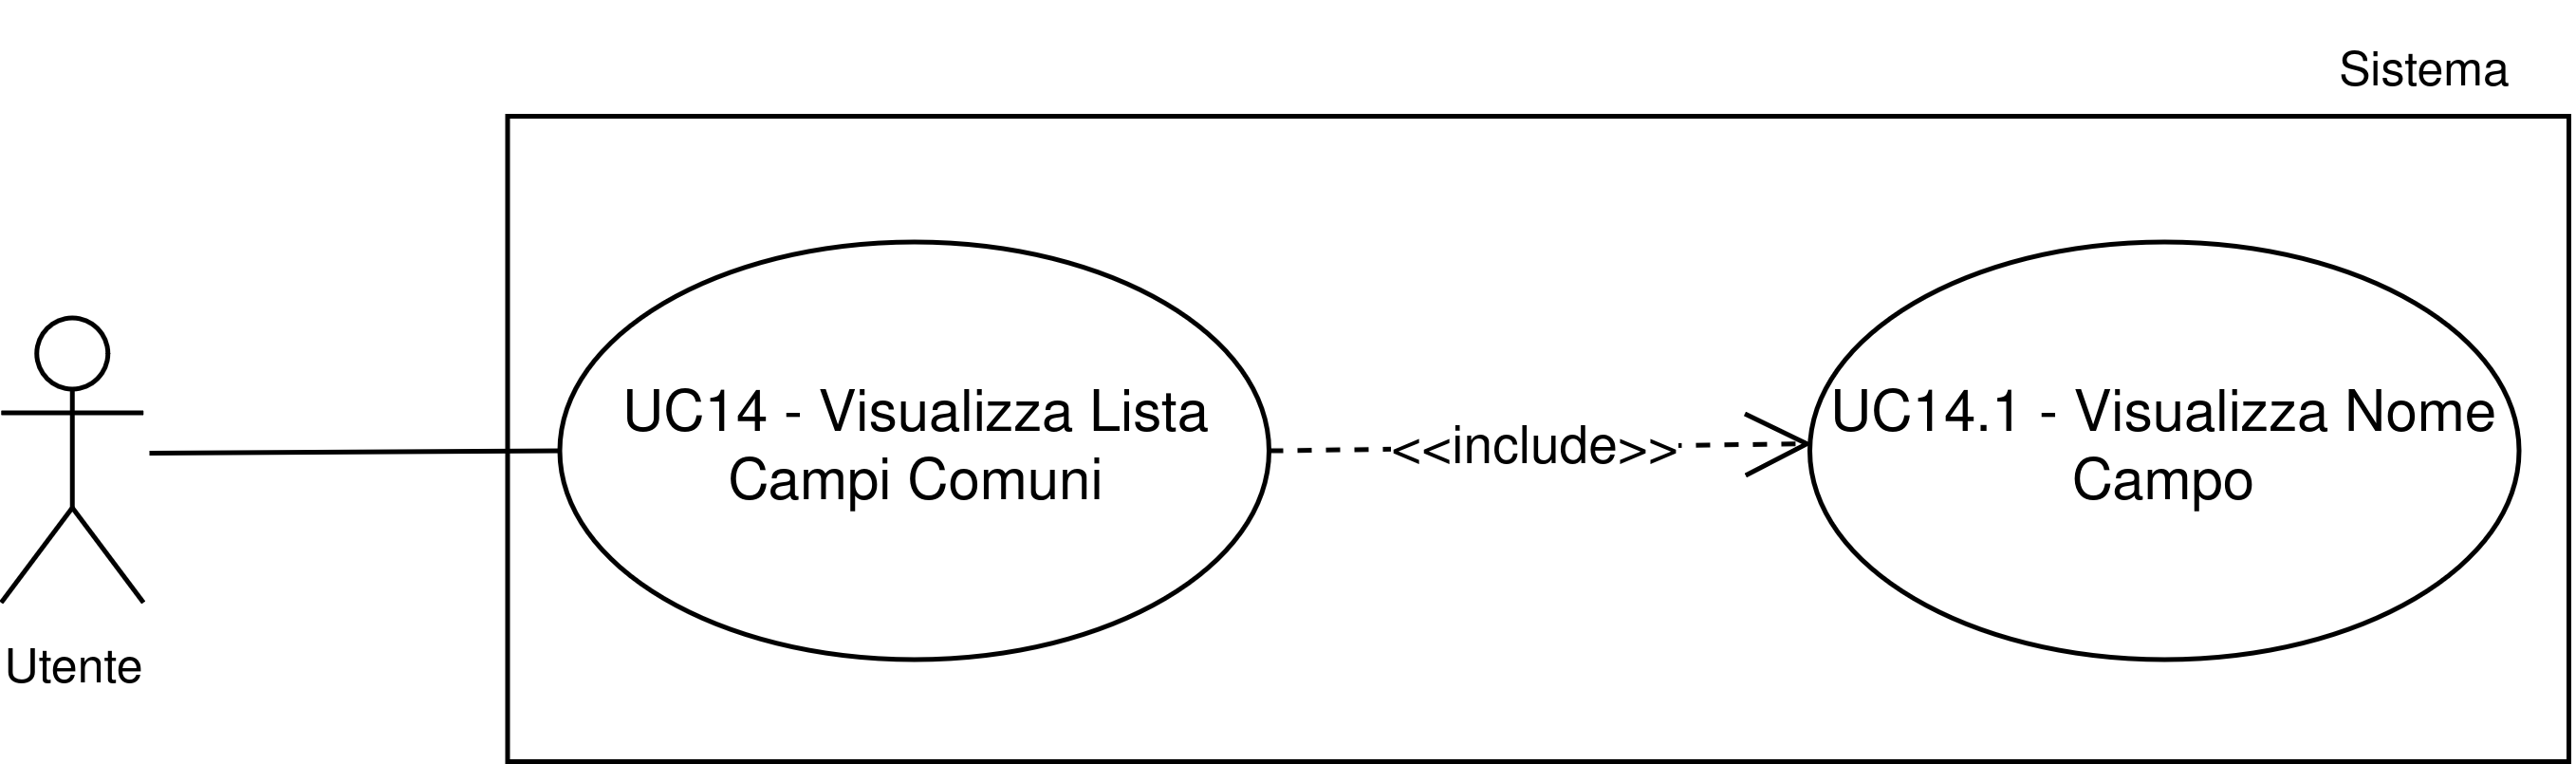
\includegraphics[width=1\textwidth]{../../assets/uml/UC14.png}
      \caption{\ref{visualizzaListaCampiComuni} - Visualizza lista campi comuni}
      \label{fig:uc_visualizzaListaCampiComuni}
\end{figure}
\begin{itemize}
      \item \textbf{Attore Primario}: Utente
      \item \textbf{Precondizioni}: 
      \begin{itemize}
            \item L'Utente ha avviato l'applicazione
            \item L'Utente sta effettuando una ricerca nel DIP con filtri
      \end{itemize}
      \item \textbf{Postcondizioni}:  L'Utente visualizza l'elenco dei campi comuni disponibili per la ricerca
      \item \textbf{Flusso Principale}:
      \begin{enumerate}
            \item Il sistema mostra a video l'elenco dei campi comuni disponibili per la ricerca e il nome corrispondente (\ref{visualizzaNomeCampo})
      \end{enumerate}
      \item \textbf{Inclusioni}: \ref{visualizzaNomeCampo} Visualizza nome del campo
\end{itemize}

\subusecase{visualizzaNomeCampo}{Visualizza nome del campo}
\begin{itemize}
      \item \textbf{Attore Primario}: Utente
      \item \textbf{Precondizioni}: 
      \begin{itemize}
            \item L'Utente ha avviato l'applicazione
            \item L'Utente sta effettuando una ricerca nel DIP con filtri
            \item L'utente sta visualizzando una lista di campi
      \end{itemize}
      \item \textbf{Postcondizioni}:  L'Utente visualizza il nome del campo
      \item \textbf{Flusso Principale}:
      \begin{enumerate}
            \item Il sistema mostra a video il nome del campo
      \end{enumerate}
\end{itemize}

\usecase{visualizzaRisultati}{Visualizza Risultati di Ricerca} \label{risultatiRicerca}
\begin{figure}[H]
      \centering
      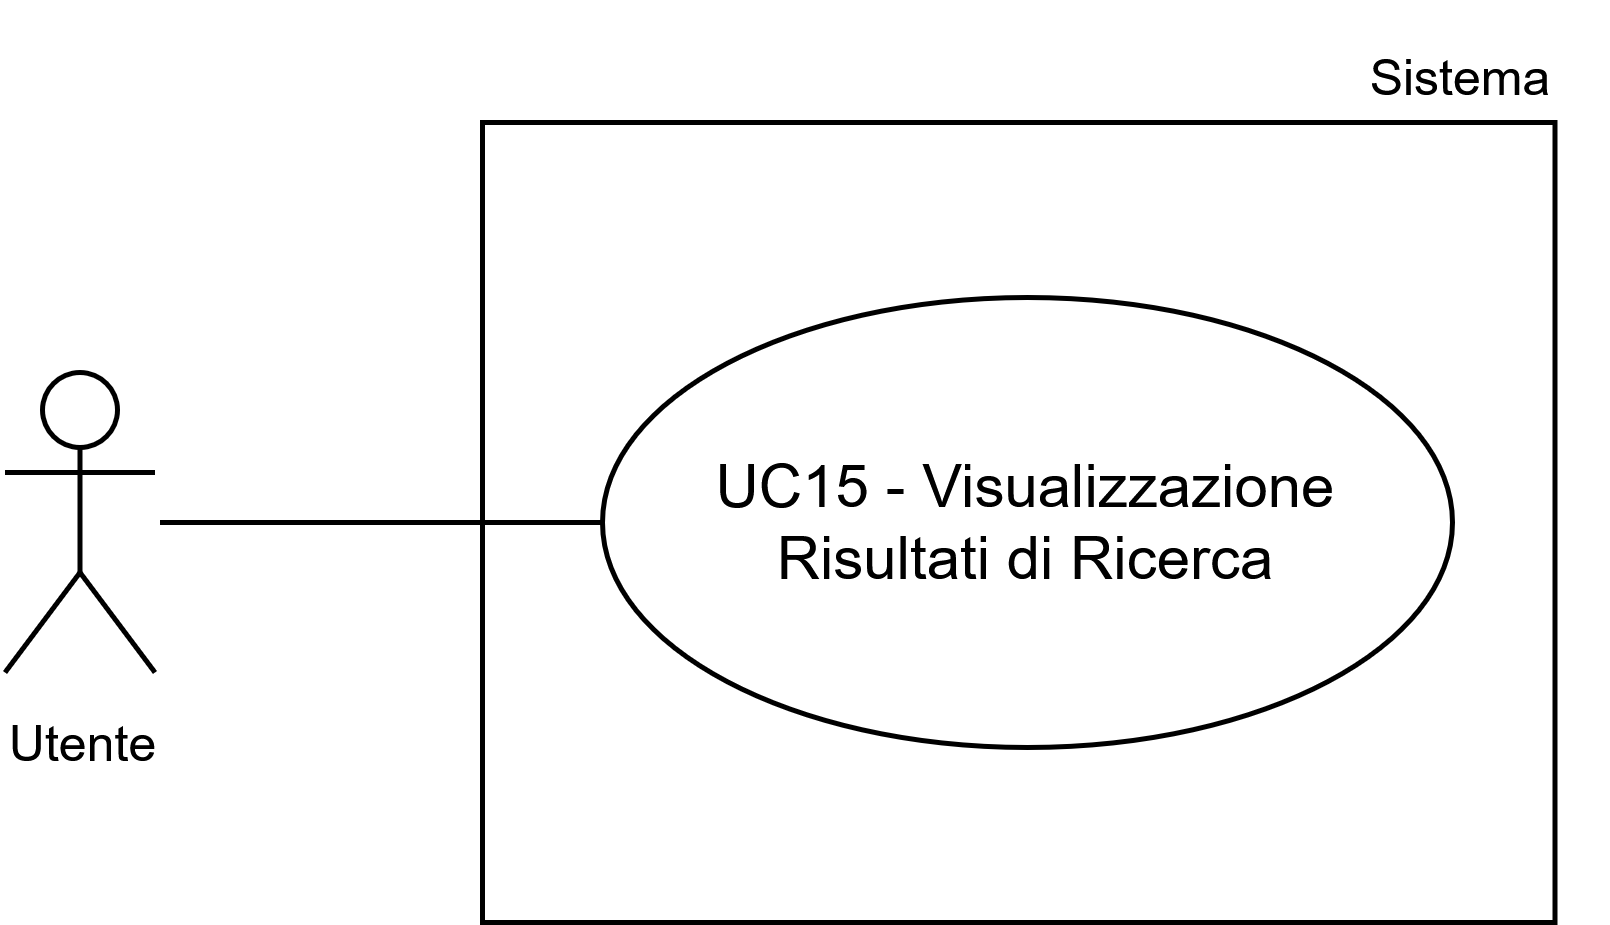
\includegraphics[width=0.6\textwidth]{../../assets/uml/UC15.png}
      \caption{\ref{visualizzaRisultati} - Visualizzazione Risultati di Ricerca}
      \label{fig:uc_VisualizzazioneRisultatiDiRicerca}
\end{figure}
\begin{itemize}
      \item \textbf{Attore Primario}: Utente
      \item \textbf{Precondizioni}: \begin{itemize}
            \item L'Utente ha avviato l'applicazione
            \item L'Utente ha eseguito una ricerca (tramite \ref{ricercaDIP} e sue specializzazioni).
      \end{itemize}
      \item \textbf{Postcondizioni}: I risultati della ricerca sono presentati all'Utente come lista di elementi.
      \item \textbf{Flusso Principale}:
      \begin{enumerate}
            \item L'Utente visualizza un elenco di elementi che corrispondono ai criteri di ricerca.
            \item Per ogni elemento, vengono mostrate le informazioni principali (Nome, Data, Tipo) (\ref{infoRisultatiRicerca})
      \end{enumerate}
      %\item \textbf{Flusso Alternativo}:
      %\begin{enumerate}
      %      \item Il sistema non trova risultati che corrispondono ai criteri di ricerca.
      %\end{enumerate}
      \item \textbf{Inclusioni}: \ref{infoRisultatiRicerca} Visualizza elemento lista risultati
      %\item \textbf{Estensioni}: \ref{nessunRisultato} Nessun Risultato
\end{itemize}
\begin{figure}[H]
      \centering
      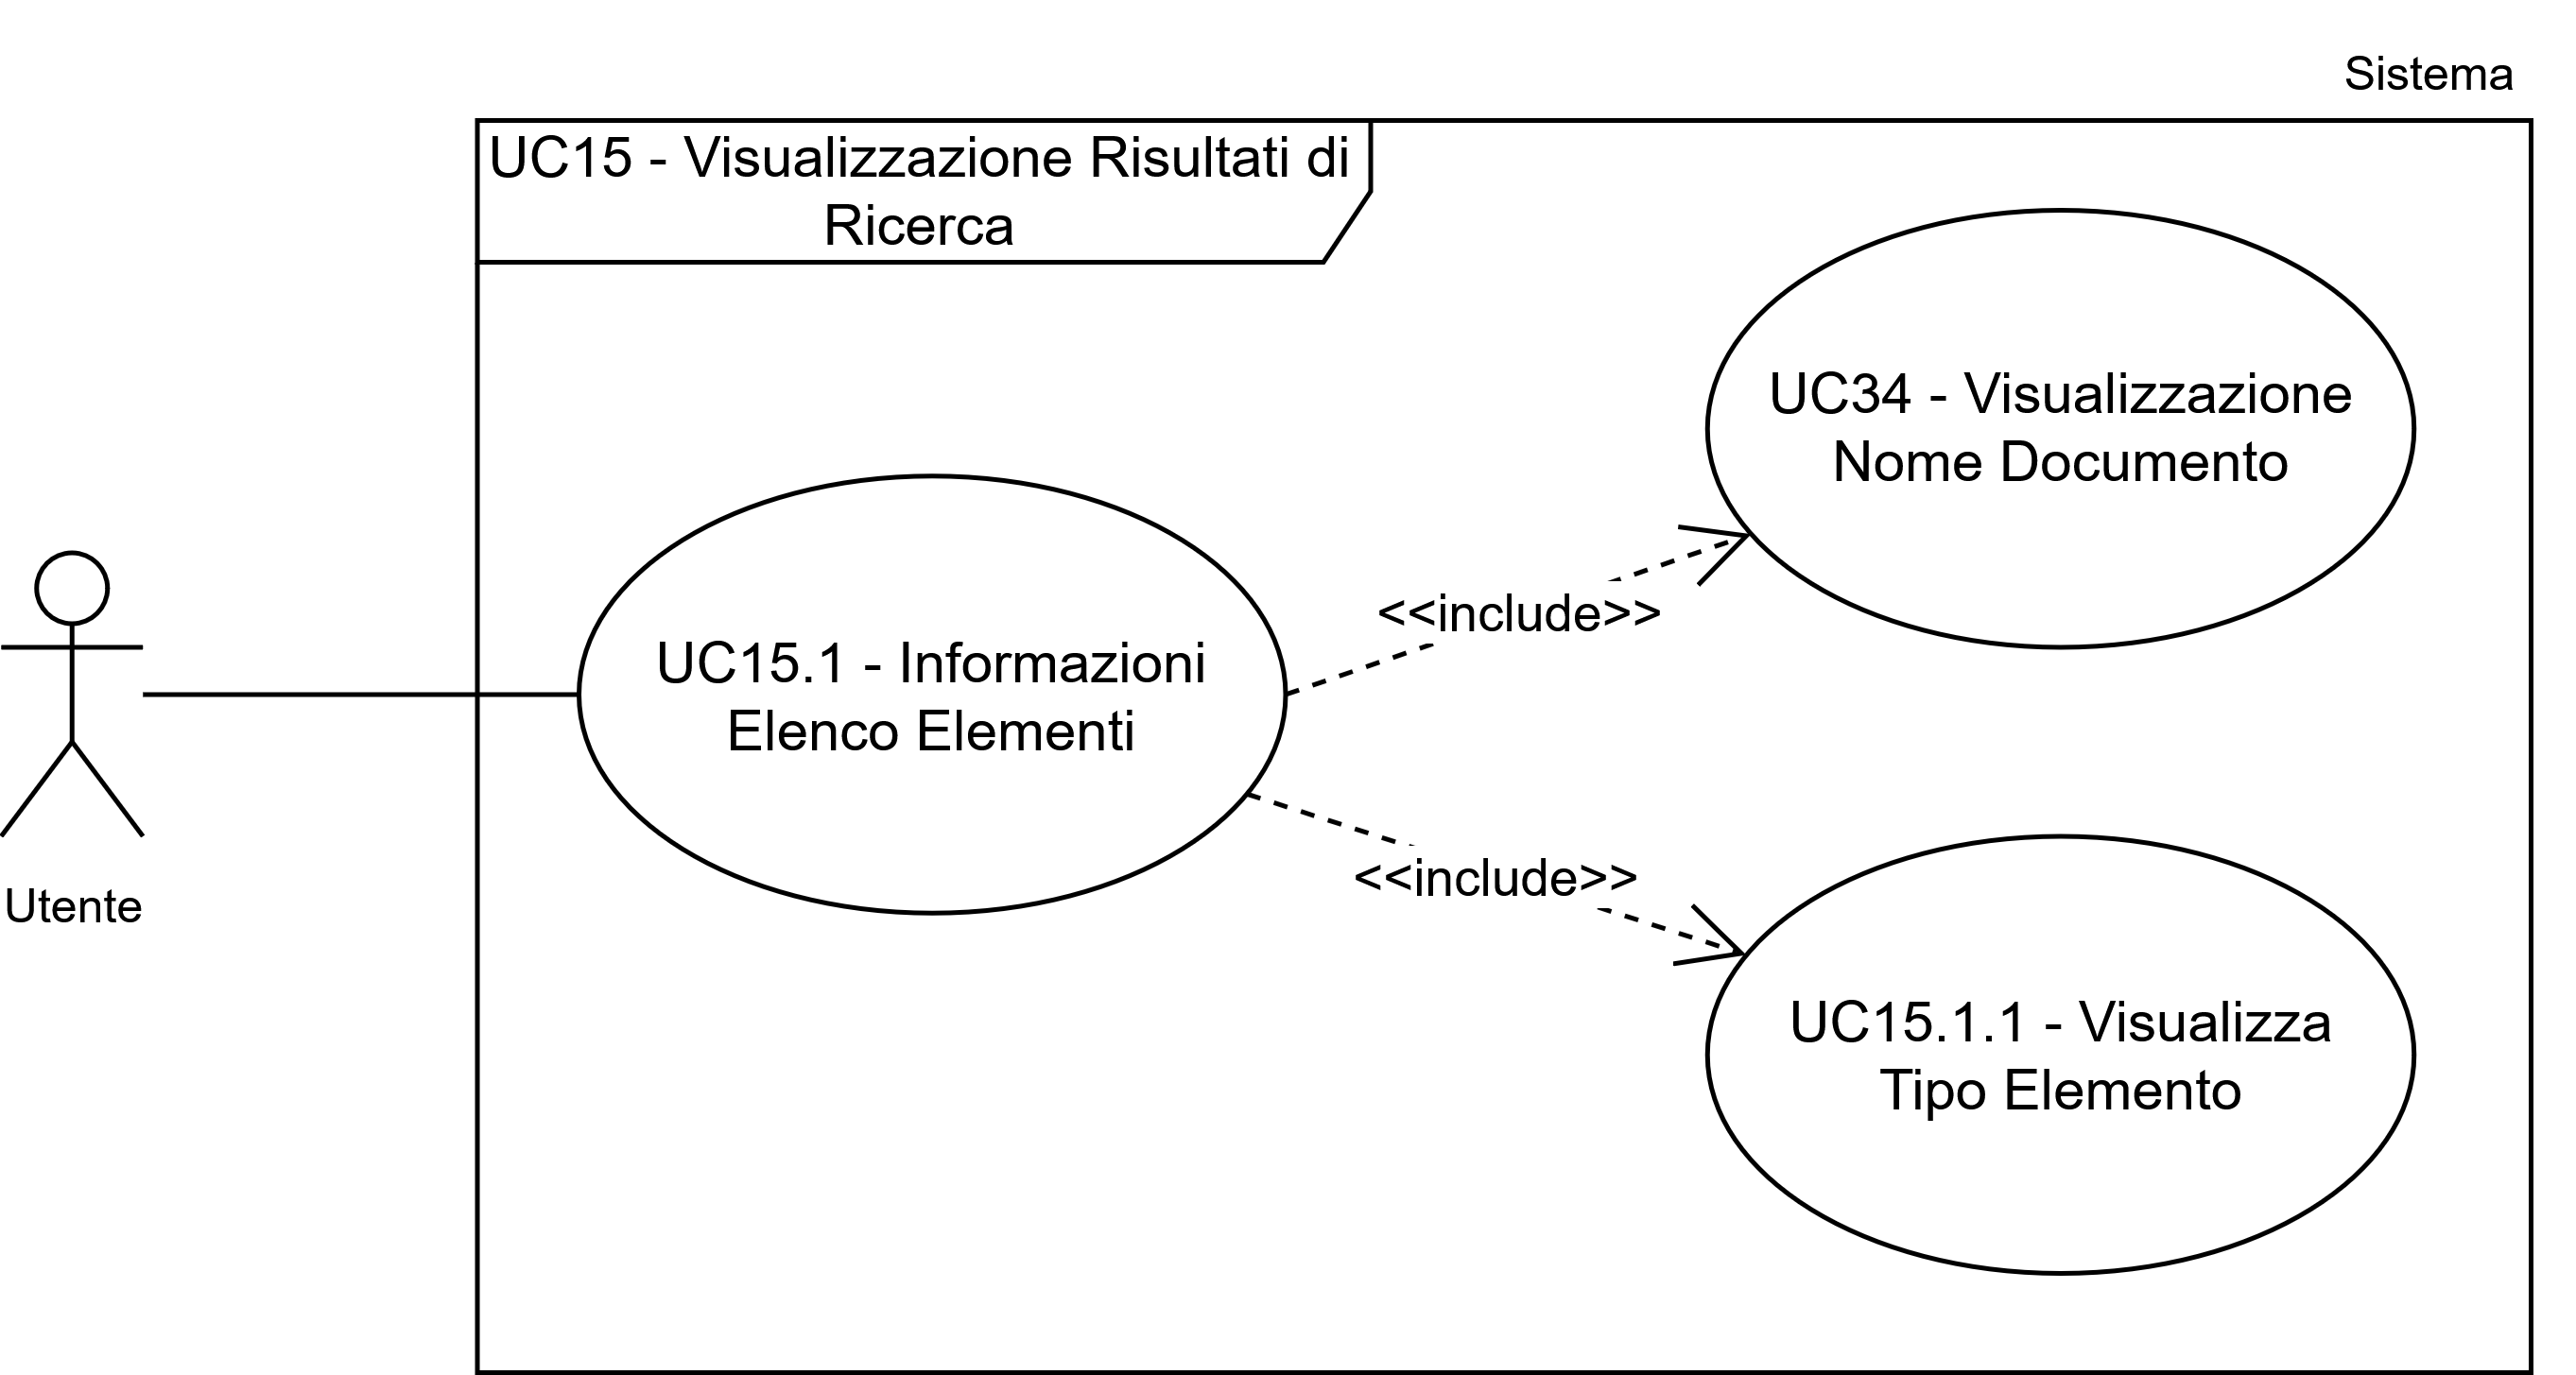
\includegraphics[width=0.9\textwidth]{../../assets/uml/UC15INC.png}
      \caption{Inclusioni \ref{visualizzaRisultati} - Visualizza elemento lista risultati}
      \label{fig:inclusioniInformazioniElencoElementi}
\end{figure}

\subusecase{infoRisultatiRicerca}{Visualizza elemento lista risultati}
\begin{itemize}
      \item \textbf{Attore Primario}: Utente
      \item \textbf{Precondizioni}: 
      \begin{itemize}
            \item L'Utente ha avviato l'applicazione
            \item L'Utente ha eseguito una ricerca (tramite \ref{ricercaDIP} e sue specializzazioni).
      \end{itemize}
      \item \textbf{Postcondizioni}: Le proprietà di un elemento della lista risultati vengono mostrate all'utente.
      \item \textbf{Flusso Principale}:
      \begin{enumerate}
            \item L'Utente visualizza il nome dell'elemento (\ref{nomeDocumentoProcesso}).
            \item L'Utente visualizza il tipo di elemento tra Documento, Aggregazione, Processo e Classe Documentale.
      \end{enumerate}
      \item \textbf{Inclusioni}:
      \begin{itemize}
            \item \ref{nomeElemento} Visualizza nome elemento
            \item \ref{visualizzaTipoElemento} Visualizza tipo elemento
      \end{itemize}
\end{itemize}

\subsubusecase{nomeElemento}{Visualizza nome elemento}
\begin{itemize}
      \item \textbf{Attore Primario}: Utente
      \item \textbf{Precondizioni}: 
      \begin{itemize}            \item L'Utente ha avviato l'applicazione
            \item L'Utente ha eseguito una ricerca (tramite \ref{ricercaDIP} e sue specializzazioni).
            \item L'Utente sta visualizzando un elemento della lista risultati.
      \end{itemize}
      \item \textbf{Postcondizioni}: L'Utente visualizza il nome dell'elemento.
      \item \textbf{Flusso Principale}:
      \begin{enumerate}
            \item Il sistema mostra a video il nome dell'elemento.
      \end{enumerate}
\end{itemize}

\subsubusecase{visualizzaTipoElemento}{Visualizza tipo elemento}
\begin{itemize}
      \item \textbf{Attore Primario}: Utente
      \item \textbf{Precondizioni}: 
      \begin{itemize}
            \item L'Utente ha avviato l'applicazione
            \item L'Utente ha eseguito una ricerca (tramite \ref{ricercaDIP} e sue specializzazioni).
            \item L'Utente sta visualizzando un elemento della lista risultati.
      \end{itemize}
      \item \textbf{Postcondizioni}: L'Utente visualizza il tipo dell'elemento tra Documento, Aggregazione, Processo e Classe Documentale.
      \item \textbf{Flusso Principale}:
      \begin{enumerate}
            \item Il sistema mostra a video il tipo dell'elemento tra Documento, Aggregazione, Processo e Classe Documentale.
      \end{enumerate}
\end{itemize}

\usecase{nessunRisultato}{Nessun Risultato}
\begin{itemize}
      \item \textbf{Attore Primario}: Utente
      \item \textbf{Precondizioni}: \begin{itemize}
            \item L'Utente ha avviato l'applicazione
            \item L'Utente ha eseguito una ricerca (tramite \ref{ricercaDIP} e sue specializzazioni).
      \end{itemize}
      \item \textbf{Postcondizioni}: Il sistema informa l'Utente che non sono stati trovati risultati.
      \item \textbf{Flusso Principale}:
      \begin{enumerate}
            \item Il sistema visualizza un messaggio che indica che la ricerca non ha prodotto alcun risultato.
      \end{enumerate}
\end{itemize}

\usecase{formatoNonCorrettoStringa}{Formato Non Corretto: stringa}
\begin{itemize}
      \item \textbf{Attore Primario}: Utente
      \item \textbf{Precondizioni}: \begin{itemize}
            \item L'Utente ha avviato l'applicazione
            \item L'Utente sta effettuando una ricerca nel DIP con filtri
            \item L'Utente sta specificando il valore alfanumerico per un metadato del filtro selezionato.
      \end{itemize}
      \item \textbf{Postcondizioni}: Il sistema informa l'Utente che il valore inserito non è alfanumerico.
      \item \textbf{Flusso Principale}:
      \begin{enumerate}
            \item Il sistema ritorna un messaggio che indica che il valore inserito deve essere alfanumerico.
      \end{enumerate}
\end{itemize}

\usecase{formatoNonCorrettoNumero}{Formato Non Corretto: numero}
\begin{itemize}
      \item \textbf{Attore Primario}: Utente
      \item \textbf{Precondizioni}: \begin{itemize}
            \item L'Utente ha avviato l'applicazione
            \item L'Utente sta effettuando una ricerca nel DIP con filtri
            \item L'Utente sta specificando il valore numerico per un metadato del filtro selezionato.
      \end{itemize}
      \item \textbf{Postcondizioni}: Il sistema informa l'Utente che il valore inserito non è numerico.
      \item \textbf{Flusso Principale}:
      \begin{enumerate}
            \item Il sistema ritorna un messaggio che indica che il valore inserito deve essere numerico.
      \end{enumerate}
\end{itemize}